
%% bare_jrnl.tex
%% V1.4b
%% 2015/08/26
%% by Michael Shell
%% see http://www.michaelshell.org/
%% for current contact information.
%%
%% This is a skeleton file demonstrating the use of IEEEtran.cls
%% (requires IEEEtran.cls version 1.8b or later) with an IEEE
%% journal paper.
%%
%% Support sites:
%% http://www.michaelshell.org/tex/ieeetran/
%% http://www.ctan.org/pkg/ieeetran
%% and
%% http://www.ieee.org/

%%*************************************************************************
%% Legal Notice:
%% This code is offered as-is without any warranty either expressed or
%% implied; without even the implied warranty of MERCHANTABILITY or
%% FITNESS FOR A PARTICULAR PURPOSE! 
%% User assumes all risk.
%% In no event shall the IEEE or any contributor to this code be liable for
%% any damages or losses, including, but not limited to, incidental,
%% consequential, or any other damages, resulting from the use or misuse
%% of any information contained here.
%%
%% All comments are the opinions of their respective authors and are not
%% necessarily endorsed by the IEEE.
%%
%% This work is distributed under the LaTeX Project Public License (LPPL)
%% ( http://www.latex-project.org/ ) version 1.3, and may be freely used,
%% distributed and modified. A copy of the LPPL, version 1.3, is included
%% in the base LaTeX documentation of all distributions of LaTeX released
%% 2003/12/01 or later.
%% Retain all contribution notices and credits.
%% ** Modified files should be clearly indicated as such, including  **
%% ** renaming them and changing author support contact information. **
%%*************************************************************************


% *** Authors should verify (and, if needed, correct) their LaTeX system  ***
% *** with the testflow diagnostic prior to trusting their LaTeX platform ***
% *** with production work. The IEEE's font choices and paper sizes can   ***
% *** trigger bugs that do not appear when using other class files.       ***                          ***
% The testflow support page is at:
% http://www.michaelshell.org/tex/testflow/



\documentclass[journal]{IEEEtran}
\usepackage{algorithm}
\usepackage{algorithmic}
\usepackage{subfig}
\makeatletter
\newcommand{\removelatexerror}{\let\@latex@error\@gobble}
\makeatother
%
% If IEEEtran.cls has not been installed into the LaTeX system files,
% manually specify the path to it like:
% \documentclass[journal]{../sty/IEEEtran}





% Some very useful LaTeX packages include:
% (uncomment the ones you want to load)


% *** MISC UTILITY PACKAGES ***
%
%\usepackage{ifpdf}
% Heiko Oberdiek's ifpdf.sty is very useful if you need conditional
% compilation based on whether the output is pdf or dvi.
% usage:
% \ifpdf
%   % pdf code
% \else
%   % dvi code
% \fi
% The latest version of ifpdf.sty can be obtained from:
% http://www.ctan.org/pkg/ifpdf
% Also, note that IEEEtran.cls V1.7 and later provides a builtin
% \ifCLASSINFOpdf conditional that works the same way.
% When switching from latex to pdflatex and vice-versa, the compiler may
% have to be run twice to clear warning/error messages.






% *** CITATION PACKAGES ***
%
%\usepackage{cite}
% cite.sty was written by Donald Arseneau
% V1.6 and later of IEEEtran pre-defines the format of the cite.sty package
% \cite{} output to follow that of the IEEE. Loading the cite package will
% result in citation numbers being automatically sorted and properly
% "compressed/ranged". e.g., [1], [9], [2], [7], [5], [6] without using
% cite.sty will become [1], [2], [5]--[7], [9] using cite.sty. cite.sty's
% \cite will automatically add leading space, if needed. Use cite.sty's
% noadjust option (cite.sty V3.8 and later) if you want to turn this off
% such as if a citation ever needs to be enclosed in parenthesis.
% cite.sty is already installed on most LaTeX systems. Be sure and use
% version 5.0 (2009-03-20) and later if using hyperref.sty.
% The latest version can be obtained at:
% http://www.ctan.org/pkg/cite
% The documentation is contained in the cite.sty file itself.






% *** GRAPHICS RELATED PACKAGES ***
%
\ifCLASSINFOpdf
   \usepackage[pdftex]{graphicx}
  % declare the path(s) where your graphic files are
  % \graphicspath{{../pdf/}{../jpeg/}}
  % and their extensions so you won't have to specify these with
  % every instance of \includegraphics
  % \DeclareGraphicsExtensions{.pdf,.jpeg,.png}
\else
  % or other class option (dvipsone, dvipdf, if not using dvips). graphicx
  % will default to the driver specified in the system graphics.cfg if no
  % driver is specified.
  % \usepackage[dvips]{graphicx}
  % declare the path(s) where your graphic files are
  % \graphicspath{{../eps/}}
  % and their extensions so you won't have to specify these with
  % every instance of \includegraphics
  % \DeclareGraphicsExtensions{.eps}
\fi
% graphicx was written by David Carlisle and Sebastian Rahtz. It is
% required if you want graphics, photos, etc. graphicx.sty is already
% installed on most LaTeX systems. The latest version and documentation
% can be obtained at: 
% http://www.ctan.org/pkg/graphicx
% Another good source of documentation is "Using Imported Graphics in
% LaTeX2e" by Keith Reckdahl which can be found at:
% http://www.ctan.org/pkg/epslatex
%
% latex, and pdflatex in dvi mode, support graphics in encapsulated
% postscript (.eps) format. pdflatex in pdf mode supports graphics
% in .pdf, .jpeg, .png and .mps (metapost) formats. Users should ensure
% that all non-photo figures use a vector format (.eps, .pdf, .mps) and
% not a bitmapped formats (.jpeg, .png). The IEEE frowns on bitmapped formats
% which can result in "jaggedy"/blurry rendering of lines and letters as
% well as large increases in file sizes.
%
% You can find documentation about the pdfTeX application at:
% http://www.tug.org/applications/pdftex





% *** MATH PACKAGES ***
%
%\usepackage{amsmath}
% A popular package from the American Mathematical Society that provides
% many useful and powerful commands for dealing with mathematics.
%
% Note that the amsmath package sets \interdisplaylinepenalty to 10000
% thus preventing page breaks from occurring within multiline equations. Use:
%\interdisplaylinepenalty=2500
% after loading amsmath to restore such page breaks as IEEEtran.cls normally
% does. amsmath.sty is already installed on most LaTeX systems. The latest
% version and documentation can be obtained at:
% http://www.ctan.org/pkg/amsmath





% *** SPECIALIZED LIST PACKAGES ***
%
%\usepackage{algorithmic}
% algorithmic.sty was written by Peter Williams and Rogerio Brito.
% This package provides an algorithmic environment fo describing algorithms.
% You can use the algorithmic environment in-text or within a figure
% environment to provide for a floating algorithm. Do NOT use the algorithm
% floating environment provided by algorithm.sty (by the same authors) or
% algorithm2e.sty (by Christophe Fiorio) as the IEEE does not use dedicated
% algorithm float types and packages that provide these will not provide
% correct IEEE style captions. The latest version and documentation of
% algorithmic.sty can be obtained at:
% http://www.ctan.org/pkg/algorithms
% Also of interest may be the (relatively newer and more customizable)
% algorithmicx.sty package by Szasz Janos:
% http://www.ctan.org/pkg/algorithmicx




% *** ALIGNMENT PACKAGES ***
%
%\usepackage{array}
% Frank Mittelbach's and David Carlisle's array.sty patches and improves
% the standard LaTeX2e array and tabular environments to provide better
% appearance and additional user controls. As the default LaTeX2e table
% generation code is lacking to the point of almost being broken with
% respect to the quality of the end results, all users are strongly
% advised to use an enhanced (at the very least that provided by array.sty)
% set of table tools. array.sty is already installed on most systems. The
% latest version and documentation can be obtained at:
% http://www.ctan.org/pkg/array


% IEEEtran contains the IEEEeqnarray family of commands that can be used to
% generate multiline equations as well as matrices, tables, etc., of high
% quality.




% *** SUBFIGURE PACKAGES ***
%\ifCLASSOPTIONcompsoc
%  \usepackage[caption=false,font=normalsize,labelfont=sf,textfont=sf]{subfig}
%\else
%  \usepackage[caption=false,font=footnotesize]{subfig}
%\fi
% subfig.sty, written by Steven Douglas Cochran, is the modern replacement
% for subfigure.sty, the latter of which is no longer maintained and is
% incompatible with some LaTeX packages including fixltx2e. However,
% subfig.sty requires and automatically loads Axel Sommerfeldt's caption.sty
% which will override IEEEtran.cls' handling of captions and this will result
% in non-IEEE style figure/table captions. To prevent this problem, be sure
% and invoke subfig.sty's "caption=false" package option (available since
% subfig.sty version 1.3, 2005/06/28) as this is will preserve IEEEtran.cls
% handling of captions.
% Note that the Computer Society format requires a larger sans serif font
% than the serif footnote size font used in traditional IEEE formatting
% and thus the need to invoke different subfig.sty package options depending
% on whether compsoc mode has been enabled.
%
% The latest version and documentation of subfig.sty can be obtained at:
% http://www.ctan.org/pkg/subfig




% *** FLOAT PACKAGES ***
%
%\usepackage{fixltx2e}
% fixltx2e, the successor to the earlier fix2col.sty, was written by
% Frank Mittelbach and David Carlisle. This package corrects a few problems
% in the LaTeX2e kernel, the most notable of which is that in current
% LaTeX2e releases, the ordering of single and double column floats is not
% guaranteed to be preserved. Thus, an unpatched LaTeX2e can allow a
% single column figure to be placed prior to an earlier double column
% figure.
% Be aware that LaTeX2e kernels dated 2015 and later have fixltx2e.sty's
% corrections already built into the system in which case a warning will
% be issued if an attempt is made to load fixltx2e.sty as it is no longer
% needed.
% The latest version and documentation can be found at:
% http://www.ctan.org/pkg/fixltx2e


%\usepackage{stfloats}
% stfloats.sty was written by Sigitas Tolusis. This package gives LaTeX2e
% the ability to do double column floats at the bottom of the page as well
% as the top. (e.g., "\begin{figure*}[!b]" is not normally possible in
% LaTeX2e). It also provides a command:
%\fnbelowfloat
% to enable the placement of footnotes below bottom floats (the standard
% LaTeX2e kernel puts them above bottom floats). This is an invasive package
% which rewrites many portions of the LaTeX2e float routines. It may not work
% with other packages that modify the LaTeX2e float routines. The latest
% version and documentation can be obtained at:
% http://www.ctan.org/pkg/stfloats
% Do not use the stfloats baselinefloat ability as the IEEE does not allow
% \baselineskip to stretch. Authors submitting work to the IEEE should note
% that the IEEE rarely uses double column equations and that authors should try
% to avoid such use. Do not be tempted to use the cuted.sty or midfloat.sty
% packages (also by Sigitas Tolusis) as the IEEE does not format its papers in
% such ways.
% Do not attempt to use stfloats with fixltx2e as they are incompatible.
% Instead, use Morten Hogholm'a dblfloatfix which combines the features
% of both fixltx2e and stfloats:
%
% \usepackage{dblfloatfix}
% The latest version can be found at:
% http://www.ctan.org/pkg/dblfloatfix




%\ifCLASSOPTIONcaptionsoff
%  \usepackage[nomarkers]{endfloat}
% \let\MYoriglatexcaption\caption
% \renewcommand{\caption}[2][\relax]{\MYoriglatexcaption[#2]{#2}}
%\fi
% endfloat.sty was written by James Darrell McCauley, Jeff Goldberg and 
% Axel Sommerfeldt. This package may be useful when used in conjunction with 
% IEEEtran.cls'  captionsoff option. Some IEEE journals/societies require that
% submissions have lists of figures/tables at the end of the paper and that
% figures/tables without any captions are placed on a page by themselves at
% the end of the document. If needed, the draftcls IEEEtran class option or
% \CLASSINPUTbaselinestretch interface can be used to increase the line
% spacing as well. Be sure and use the nomarkers option of endfloat to
% prevent endfloat from "marking" where the figures would have been placed
% in the text. The two hack lines of code above are a slight modification of
% that suggested by in the endfloat docs (section 8.4.1) to ensure that
% the full captions always appear in the list of figures/tables - even if
% the user used the short optional argument of \caption[]{}.
% IEEE papers do not typically make use of \caption[]'s optional argument,
% so this should not be an issue. A similar trick can be used to disable
% captions of packages such as subfig.sty that lack options to turn off
% the subcaptions:
% For subfig.sty:
% \let\MYorigsubfloat\subfloat
% \renewcommand{\subfloat}[2][\relax]{\MYorigsubfloat[]{#2}}
% However, the above trick will not work if both optional arguments of
% the \subfloat command are used. Furthermore, there needs to be a
% description of each subfigure *somewhere* and endfloat does not add
% subfigure captions to its list of figures. Thus, the best approach is to
% avoid the use of subfigure captions (many IEEE journals avoid them anyway)
% and instead reference/explain all the subfigures within the main caption.
% The latest version of endfloat.sty and its documentation can obtained at:
% http://www.ctan.org/pkg/endfloat
%
% The IEEEtran \ifCLASSOPTIONcaptionsoff conditional can also be used
% later in the document, say, to conditionally put the References on a 
% page by themselves.




% *** PDF, URL AND HYPERLINK PACKAGES ***
%
%\usepackage{url}
% url.sty was written by Donald Arseneau. It provides better support for
% handling and breaking URLs. url.sty is already installed on most LaTeX
% systems. The latest version and documentation can be obtained at:
% http://www.ctan.org/pkg/url
% Basically, \url{my_url_here}.




% *** Do not adjust lengths that control margins, column widths, etc. ***
% *** Do not use packages that alter fonts (such as pslatex).         ***
% There should be no need to do such things with IEEEtran.cls V1.6 and later.
% (Unless specifically asked to do so by the journal or conference you plan
% to submit to, of course. )


% correct bad hyphenation here
\hyphenation{op-tical net-works semi-conduc-tor}


\begin{document}
%
% paper title
% Titles are generally capitalized except for words such as a, an, and, as,
% at, but, by, for, in, nor, of, on, or, the, to and up, which are usually
% not capitalized unless they are the first or last word of the title.
% Linebreaks \\ can be used within to get better formatting as desired.
% Do not put math or special symbols in the title.
\title{Simple Feedback Driven Accuracy Based\\ Reputation Mechanism for IoV}
%
%
% author names and IEEE memberships
% note positions of commas and nonbreaking spaces ( ~ ) LaTeX will not break
% a structure at a ~ so this keeps an author's name from being broken across
% two lines.
% use \thanks{} to gain access to the first footnote area
% a separate \thanks must be used for each paragraph as LaTeX2e's \thanks
% was not built to handle multiple paragraphs
%
%TODO: should i say geelong like in Dr. Doss's latest paper or Burwood?
%TODO: get Dr. Jiang's IEEE membership category.
\author{Rohan~Dahiya,
        Frank~Jiang,
        and~Robin~Doss,~\IEEEmembership{Senior Member,~IEEE}% <-this % stops a space
\thanks{R. Dahiya was a visiting researcher at the School of Info Technology, Deakin University, Burwood, VIC 3125, Australia, and is a student at Vellore Institute of Technology, Vellore, TN 632014, India. e-mail: rohandahiya@outlook.in}% <-this % stops a space
\thanks{F. Jiang and R. Doss are with School of Info Technology, Deakin University, Geelong, VIC 3220, Australia}% <-this % stops a space
\thanks{Manuscript received MonthTODO 19, 2020; revised Month 26, 2020.(PLACEHOLDER)}}

% note the % following the last \IEEEmembership and also \thanks - 
% these prevent an unwanted space from occurring between the last author name
% and the end of the author line. i.e., if you had this:
% 
% \author{....lastname \thanks{...} \thanks{...} }
%                     ^------------^------------^----Do not want these spaces!
%
% a space would be appended to the last name and could cause every name on that
% line to be shifted left slightly. This is one of those "LaTeX things". For
% instance, "\textbf{A} \textbf{B}" will typeset as "A B" not "AB". To get
% "AB" then you have to do: "\textbf{A}\textbf{B}"
% \thanks is no different in this regard, so shield the last } of each \thanks
% that ends a line with a % and do not let a space in before the next \thanks.
% Spaces after \IEEEmembership other than the last one are OK (and needed) as
% you are supposed to have spaces between the names. For what it is worth,
% this is a minor point as most people would not even notice if the said evil
% space somehow managed to creep in.



% The paper headers
\markboth{Journal of \LaTeX\ Class Files,~Vol.~14, No.~8, August~2015(PLACEHOLDER)}%
{Shell \MakeLowercase{\textit{et al.}}: Bare Demo of IEEEtran.cls for IEEE Journals}
% The only time the second header will appear is for the odd numbered pages
% after the title page when using the twoside option.
% 
% *** Note that you probably will NOT want to include the author's ***
% *** name in the headers of peer review papers.                   ***
% You can use \ifCLASSOPTIONpeerreview for conditional compilation here if
% you desire.




% If you want to put a publisher's ID mark on the page you can do it like
% this:
%\IEEEpubid{0000--0000/00\$00.00~\copyright~2015 IEEE}
% Remember, if you use this you must call \IEEEpubidadjcol in the second
% column for its text to clear the IEEEpubid mark.



% use for special paper notices
%\IEEEspecialpapernotice{(Invited Paper)}




% make the title area
\maketitle

% As a general rule, do not put math, special symbols or citations
% in the abstract or keywords.
\begin{abstract}
Several mechanisms have been proposed for trust management in SIoV. Most of these employ reputation as an important factor. There have also been various mechanisms proposed for detection of false information being shared in IoVs in various applications. The advent of 5G is expected to enable fast communication between nodes in an IoV thereby removing previously limiting factors on applications. We propose and evaluate a reputation mechanism for IoV that uses false information detection mechanisms to generate feedback and uses this feedback, after filtration/vetting, to generate a reputation score that may be used as part of a trust management system or as a factor in a false message detection system.
\end{abstract}

% Note that keywords are not normally used for peerreview papers.
\begin{IEEEkeywords}
IoV, VANET, V2X, Reputation System, Trust Management.
\end{IEEEkeywords}






% For peer review papers, you can put extra information on the cover
% page as needed:
% \ifCLASSOPTIONpeerreview
% \begin{center} \bfseries EDICS Category: 3-BBND \end{center}
% \fi
%
% For peerreview papers, this IEEEtran command inserts a page break and
% creates the second title. It will be ignored for other modes.
\IEEEpeerreviewmaketitle



\section{Introduction}

% The very first letter is a 2 line initial drop letter followed
% by the rest of the first word in caps.
% 
% form to use if the first word consists of a single letter:
% \IEEEPARstart{A}{demo} file is ....
% 
% form to use if you need the single drop letter followed by
% normal text (unknown if ever used by the IEEE):
% \IEEEPARstart{A}{}demo file is ....
% 
% Some journals put the first two words in caps:
% \IEEEPARstart{T}{his demo} file is ....
% 
% Here we have the typical use of a "T" for an initial drop letter
% and "HIS" in caps to complete the first word.
\IEEEPARstart{V}{ehicular} ad-hoc networks (VANETs) which have been around for decades are based on the principles of mobile ad-hoc networks (MANETs) being applied to the domain of vehicles and infrastructure. They consist of On Board Units (OBUs) in vehicles (peers/nodes) and Road Side Units (RSUs). Internet of Vehicles (IoV) is a concept that is derived from VANETs where each node and RSU is internet enabled and is capable of communicating with each other via dedicated short-range communication (DSRC). Numerous uses of IoV have been proposed from infotainment to traffic safety related applications such as traffic information sharing, emergency vehicle notification systems and collision avoidance systems.
\\5G, the fifth generation technology standard for cellular networks \cite{c:INTERNET_5garticle}, began being deployed in 2019 and mid-band 5G (which offers much higher data transfer rates) were expected to be available in most metropolitan areas by 2020. In Europe, a consortium of companies, is helping to develop a 5G system architecture to provide optimized end-to-end vehicle to everything (V2X) connectivity called the 5GCAR project.
V2X is an umbrella term that refers to a combination of more specific types of communication as V2I (vehicle-to-infrastructure), V2N (vehicle-to-network), V2V (vehicle-to-vehicle), V2P (vehicle-to-pedestrian), V2D (vehicle-to-device) and V2G (vehicle-to-grid). 5G can be expected to mitigate some of the limitations in IoV and pave the way for applications that would not have been plausible before.
\\Most application in IoV rely on cooperativeness of other nodes to function especially applications that are based on the exchange of information between nodes. False information being shared by malicious nodes can negatively affect the utility of these applications. For this reason, trust management systems and reputation mechanisms are employed in Social Internet of Vehicles (SIoV) to quantify the reliability of information received.
\\ The scope of this paper is to introduce a primarily centralised reputation mechanism that aims to accurately estimate the accuracy of a nodes messages based on feedback from other nodes while filtering out false feedback. A review of related works on attacks in IoV, False information detection systems and trust management systems is presented in Sections \ref{sec:RV:attacks}, \ref{sec:RV:FalseMsgDetection} and \ref{sec:RV:trust&Reputation} respectively. The proposed methods are described in Section \ref{sec:PM}. The proposed methods were tested via software simulation, details on the experiments and the observations are presented in Section \ref{sec:Experiments} and Section \ref{sec:Results} respectively, and the conclusion is contained in Section \ref{sec:Conclusion}.

%\hfill mds
 
%\hfill August 26, 2015


% needed in second column of first page if using \IEEEpubid
%\IEEEpubidadjcol



% An example of a floating figure using the graphicx package.
% Note that \label must occur AFTER (or within) \caption.
% For figures, \caption should occur after the \includegraphics.
% Note that IEEEtran v1.7 and later has special internal code that
% is designed to preserve the operation of \label within \caption
% even when the captionsoff option is in effect. However, because
% of issues like this, it may be the safest practice to put all your
% \label just after \caption rather than within \caption{}.
%
% Reminder: the "draftcls" or "draftclsnofoot", not "draft", class
% option should be used if it is desired that the figures are to be
% displayed while in draft mode.
%
%\begin{figure}[!t]
%\centering
%\includegraphics[width=2.5in]{myfigure}
% where an .eps filename suffix will be assumed under latex, 
% and a .pdf suffix will be assumed for pdflatex; or what has been declared
% via \DeclareGraphicsExtensions.
%\caption{Simulation results for the network.}
%\label{fig_sim}
%\end{figure}

% Note that the IEEE typically puts floats only at the top, even when this
% results in a large percentage of a column being occupied by floats.


% An example of a double column floating figure using two subfigures.
% (The subfig.sty package must be loaded for this to work.)
% The subfigure \label commands are set within each subfloat command,
% and the \label for the overall figure must come after \caption.
% \hfil is used as a separator to get equal spacing.
% Watch out that the combined width of all the subfigures on a 
% line do not exceed the text width or a line break will occur.
%
%\begin{figure*}[!t]
%\centering
%\subfloat[Case I]{\includegraphics[width=2.5in]{box}%
%\label{fig_first_case}}
%\hfil
%\subfloat[Case II]{\includegraphics[width=2.5in]{box}%
%\label{fig_second_case}}
%\caption{Simulation results for the network.}
%\label{fig_sim}
%\end{figure*}
%
% Note that often IEEE papers with subfigures do not employ subfigure
% captions (using the optional argument to \subfloat[]), but instead will
% reference/describe all of them (a), (b), etc., within the main caption.
% Be aware that for subfig.sty to generate the (a), (b), etc., subfigure
% labels, the optional argument to \subfloat must be present. If a
% subcaption is not desired, just leave its contents blank,
% e.g., \subfloat[].


% An example of a floating table. Note that, for IEEE style tables, the
% \caption command should come BEFORE the table and, given that table
% captions serve much like titles, are usually capitalized except for words
% such as a, an, and, as, at, but, by, for, in, nor, of, on, or, the, to
% and up, which are usually not capitalized unless they are the first or
% last word of the caption. Table text will default to \footnotesize as
% the IEEE normally uses this smaller font for tables.
% The \label must come after \caption as always.
%
%\begin{table}[!t]
%% increase table row spacing, adjust to taste
%\renewcommand{\arraystretch}{1.3}
% if using array.sty, it might be a good idea to tweak the value of
% \extrarowheight as needed to properly center the text within the cells
%\caption{An Example of a Table}
%\label{table_example}
%\centering
%% Some packages, such as MDW tools, offer better commands for making tables
%% than the plain LaTeX2e tabular which is used here.
%\begin{tabular}{|c||c|}
%\hline
%One & Two\\
%\hline
%Three & Four\\
%\hline
%\end{tabular}
%\end{table}


% Note that the IEEE does not put floats in the very first column
% - or typically anywhere on the first page for that matter. Also,
% in-text middle ("here") positioning is typically not used, but it
% is allowed and encouraged for Computer Society conferences (but
% not Computer Society journals). Most IEEE journals/conferences use
% top floats exclusively. 
% Note that, LaTeX2e, unlike IEEE journals/conferences, places
% footnotes above bottom floats. This can be corrected via the
% \fnbelowfloat command of the stfloats package.

\section{Related Works}
\label{sec:RV}
\subsection{Attacks in IoV}
\label{sec:RV:attacks}
A survey of various attacks and detection mechanisms on VANETs and IoVs has been done by Sakiz et al. \cite{c:AttacksSurvey}. A brief description of the various attacks described is as follows.
\begin{itemize}
	\item \textbf{Sybil Attack} A node pretends to have more then one identity.
	\item \textbf{DoS Attack} A Denial of Service or Distributed Denial of service attack aims to render the service unavailable by means of jamming, flooding etc.
	\item \textbf{Blackhole Attack} A node sends false routing information to make all other nodes try to route their packets through it, the packets are then dropped.
	\item \textbf{Wormhole Attack} Similar to black-hole attack, in a wormhole attack, two compromised nodes forward packets between each other after encapsulating them therefore the hop count is not affected. This makes these two nodes appear as the best route to send any packets.
	\item \textbf{Bogus Information Attack} A type of soft attack where a malicious node sends false information in the network.
	\item \textbf{Replay Attack} An attacker replays a message that was sent earlier out of context. Unlikely with the use of timestamps.
\end{itemize}
The bogus information attack mentioned above is based on the fact that vehicles in an IoV share information among each other and use that information in various protocols. In this attack a malicious node disseminates false information with the aim of manipulating the behaviour of other nodes, this effect is increased if the attacker is moving around swiftly\cite{c:MotorwayAttack}. Various variations of this attack have been studied by Sakiz et al.\cite{c:AttacksSurvey} such as False Position Information\cite{c:FalsePositionInformation}, Sensor Tampering, Illusion Attack\cite{c:IllusionAttack} and GPS Spoofing/Tunnel Attack\cite{c:TunnelAttack}. Various methods have been proposed for the detection of false messages as described in the following subsection (\ref{sec:RV:FalseMsgDetection}). These can help a vehicle identify which messages to ignore and the results of these methods could further be used to detect and purge attackers from the network for which voting, evaluation and reputation based mechanisms have been suggested\cite{c:MDSandLEAVE}(\textit{Local Eviction of Attackers by Voting Evaluators})\cite{c:messagefilterCoE}. 

\subsection{False Message Detection}
\label{sec:RV:FalseMsgDetection}
Lo et al. \cite{c:IllusionAttack} propose a mechanism called \textit{Plausibility Validation Network (PVN)} which is capable of checking the data received from sensors, or other vehicles, and validating it. It includes a plausibility network and a rule database. For each category of messages the various rules are used to detect information that logically must be false based on known truths.
Another  message filtering model is proposed by Kim et al. \cite{c:messagefilterCoE}. The model includes a threshold curve and a certainty of event (CoE) curve. The CoE, which indicates the confidence level of a received message, is calculated by combining the data from various sources such as local sensors, RSUs and reputation mechanism. The solution relies on honest majority. The threshold curve shows the insensitivity of the driver with respect to the distance to the event. Sensitivity and the distance to the event are inversely proportional. Therefore, while the threshold value is decreasing, the CoE value keeps increasing and, if it exceeds the threshold value which is assigned according to the application, the driver is warned with an alert message. The paper suggested the use of a rudimentary reputation system as an input factor for the CoE score among five other factors.
\subsection{Trust Management and Reputation}
\label{sec:RV:trust&Reputation}
Iqbal et al. \cite{c:trustInSIoV} enumerated various factors involved in the conceptualisation of a trust system in SIoV, which differs from IoV by the fact that objects in SIoV maintain social relationships. Trust management mechanism in SIoV serves the purpose of establishing a node as trustworthy and to gauge the trustworthiness of other nodes in the network. The eight main factors enumerated for evaluation of trust were:\\
	\begin{enumerate}
		\item Reputation - Score based on feedback.
		\item Context
		\item Environment
		\item Goals
		\item User expectations
		\item Social relationships
		\item Willingness to connect
		\item Timeliness of evaluation 
	\end{enumerate}
Of these eight factors, reputation plays a fundamental role. Various methods have been proposed of a reputation mechanism in VANETs. The utility of various reputation mechanisms proposed for MANETs is limited in VANETs due to the dynamic nature of the network where no two nodes are in range of each other for long periods. Various reputation mechanisms have been proposed for specific applications such as location verification\cite{c:positionVerificationRepMech}. The importance of a decentralised system for trust management in VANETs\cite{c:Huang_decentrTrustMechVANETS} has been recognised among other previous efforts surveyed by Soleymani et al.\cite{c:trustinVANETsurvey}.
\section{Proposed Methods}
\label{sec:PM}
With the advent of 5G networks enabling rapid 2-way communication, we propose a primarily centralised system that leverages this connectivity for reputation score generation based on accuracy of information shared, where the information is not restricted to any specific type or application as long as it can be evaluated to be true or false by a node. The aim of this mechanism is to accurately predict the accuracy of information from sources based on feedback on that information and to filter out false feedback. This reputation mechanism may then be used as a sub module of a multi-factor trust management system.
We describe our proposed system for reputation score generation in this section as well as propose methods of sharing feedback to the network and usage of the scores. \\ We have divided the section into three subsections. The first subsection details how the feedback is created, propagated and collected in the network, in the second sub-section, methods of score generation are described and the third sub-section details the proposed method for the distribution/application of the scores generated. It is assumed that the RSUs can communicate with each other and therefore can distribute the computation and maintain shared storage in the from of IPFS etc.
%(TODO add citation?)
However, the details of it are beyond the scope of this article. For simplicity the network of RSUs is referred to as a single unit henceforth in this section.
\subsection{Feedback Generation and Collection}
\label{sec:PM:FeedbackGen&Collect}
Nodes in an IoV may be able to classify some of the information they receive as true or false either by means of self observation or context aware deduction using primarily data centric methods of false information detection such as the those proposed by Kim et al.\cite{c:messagefilterCoE} and Lo et al.\cite{c:IllusionAttack}, as previously mentioned in Section \ref{sec:RV:FalseMsgDetection}. If a message is determined to be true or false by a receiving node, it can share feedback on it with the other nodes of the network. The usage of this feedback is detailed in subsequent subsections. In the proposed system feedback is shared primarily in the form of a report comprising of 4 elements: the reportee's id (or address), the reporter's id (or address), the message id (or a unique message identifier), and a boolean value used to indicate if the message being reported on was found to be true or false by the reporter. 
\subsubsection{Feedback Generation by Nodes}
The feedback exchange in the network is triggered by the following events:
\begin{itemize}
	\item \textbf{Message Classified:} Whenever the truthfulness of a received message is determined, a report is created and shared on the network.
	\item \textbf{Message received from a sender for the first time:} In order to bring new nodes joining a network up to par with the rest of the network, whenever a node $ a $ receives a message from a node $ b $ on which it has no feedback information, it ($ a $) sends a "Request for Reports" message containing only $ b $'s id.
	\item \textbf{Request for Reports Received:} When a Request for Reports on any node $ b $ is received by some node $ a $, it sends a "Reports Dump" message containing all the reports it has sent on $ b $ that it contains in storage.
\end{itemize}
\subsubsection{Feedback Collection at RSU}
Three lists of messages are maintained: Current Scope, Staged Scope and Archived Scope.
Two data objects, referred to as baskets, are used to store and process the reports received, all reports that are received are put into one of two baskets:
\begin{enumerate}
	\item \textbf{Current Basket}: if the message that the report is on is not in Staged Scope or Archived Scope, the message is added to the Current Scope and the report is collected in the Current Basket.
	\item \textbf{Staged Basket}: Only reports on messages that are listed in the staged scope are collected in the staged basket.
\end{enumerate}
If a report is received on a message that is in the Archived Scope, it is ignored. Each basket stores the reports that are inserted in it and it's implementation can include variables to maintain some metadata on the reports to facilitate the score generation process which is detailed later. At regular intervals of time, which roughly equals the average amount of time between a node sending a message and another node receiving a report on that message, a "Stage Shift" event is triggered. When Stage shift occurs the elements of the staged scope are added to archived scope. Secondary scores and fuzzy truth-values of messages are calculated based on the contents of the staged basket before it is emptied, this process is elaborated in following subsections. These truth-values are then inserted into logs, which is used to generate the primary scores. After this the contents of the Current Basket are shifted to the Staged Basket before it is emptied. Corresponding operations are performed on the staged and current scope lists. 
The logs for each vehicle contain the calculated truth-values of messages sent by it, and other counters that are used to calculate the primary scores for it with optimal complexity.
It can be summarised that the archived scope is the list of messages for which the truth-values have been calculated and inserted into the logs, the staged scope is the list of messages for which the reports are still being collected and that will be processed and inserted into logs at the next stage shift event, and the current scope is the expanding list of messages that will form the fixed staged scope list at the next stage shift event.
\subsubsection{RSU Results Broadcasting and incorporation at Nodes}
As mentioned previously, the logs at the RSU contain the calculated truth-values of messages which are used to generate the Primary Scores, the calculation of these truth-values and Primary Scores is detailed in the subsequent subsection.
In order to share it's results the RSU calculates the primary score of each node for various window sizes i.e [10,50,250,1250] or such and sends these (with other metadata) along with the list of blacklisted nodes in a message to all nodes in the network. Whenever a message from an RSU is received the node can make a copy of the blacklist to ignore reports from the blacklisted nodes, until the blacklist is updated again and it can insert dummy messages/reports from various nodes into it's own storage by reverse calculating from the received primary scores and metadata in order to emulate the same knowledge.
\subsection{Score Generation}
\label{sec:PM:ScoreGeneretion}
We describe the method of score-generation in this subsection. All data pertaining to reports and counters in this subsection and in Figures \ref{fig:ALG_ss} to \ref{fig:ALG_PSCalc} refers to the data collected in the staged basket up until the stage shift event occurs and the various score generation methods are called, unless otherwise specified to refer to data in Logs. 
In order to generate an estimate of the overall accuracy of all the information shared by a node, the system calculates a truth-value for each message sent by that node based on all the feedback on that message, then the mean of the truth-values of a set of messages is taken. This estimate of the overall accuracy of a node is referred to as the Primary Score or the Reputation Score interchangeably in this article. Since the feedback may be deliberately falsified as well, it is first necessary to exclude the feedback from nodes that may be malicious. In order to distinguish nodes with false feedback another parameter is used which is referred to as the "Secondary Score" for a node.
The following sub-sub-sections describe the methods for ultimately generating the Primary Score for each node.
%\subsubsection{Reports Based (RAW) Score Generation}

\subsubsection{Secondary Score Generation}
When ever a new report is received by the RSU, counters corresponding to the number of positive and negative reports on a node and the number of positive and negative reports from a node on another node can be incremented. These counters can then be utilised to quickly calculate each node's median implied reputation score (MI Score), which is defined as the median of all the implied reputation scores for that node, where an implied reputation score of a node is the fraction of positive reports to total reports by another node. See Fig. \ref{fig:ALG_ss}, Alg. \ref{algo:mi}.
\begin{figure}[!t]\removelatexerror
	\caption{Calculation of Secondary Scores} 
	\label{fig:ALG_ss}
\begin{algorithm}[H]
	\caption{Calculate Median Implied Scores}  
	\label{algo:mi} 
	\textbf{INPUT:} 
	\begin{enumerate}
		\item $N$: Set of all nodes on which at least one report was received
		\item $Count^{Total}_{i,j}$: Count of Total Reports on node $ i $ by node $ j \ \forall i,j\in N $
		\item $Count^{Positive}_{i,j}$: Count of Positive Reports on node $ i $ by node $ j \ \forall i,j\in N $
	\end{enumerate}
	\textbf{OUTPUT:}  $Score^{MIS}_n$: Median Implied Score of node $n\ \forall n\in N$
	\begin{algorithmic}[1]
		\FORALL{$i\ \in\ N$}
			\STATE $impliedScore_{j} \leftarrow Count^{Positive}_{i,j} / Count^{Total}_{i,j}$\\$\forall j \in N-\{i\} $
			\STATE $ Score^{MIS}_i \leftarrow$ median($impliedScore_j\ \forall\ j\in N-\{i\}$)
		\ENDFOR
		\RETURN $Score^{MIS}_i\ \forall i\in N$
	\end{algorithmic}
	\textbf{Complexity:} $\mathcal{O}(n^2)$.
\end{algorithm}
\begin{algorithm}[H]
	\caption{Calculate Secondary Scores}
	\label{algo:SSCalc}
	\textbf{INPUT:} 
	\begin{enumerate}
		\item $N$: Set of all nodes from whom at-least 1 report was received
		\item $Count^{Total}_{i,j}$: Count of Total Reports on node $ n $ by node $ j \ \forall i,j\in N $
		\item $Count^{Positive}_{i,j}$: Count of Positive Reports on node $ n $ by node $ j \ \forall i,j\in N $
		\item $Score^{MI}_n$: MI Score of node $n\ \forall n\in N$
	\end{enumerate}
	\textbf{OUTPUT:} $Score^{Secondary}_n$: Secondary Score of node $n\ \forall n\in N$
	\begin{algorithmic}
		\FORALL{$i\ \in\ N$}
			\STATE $TSE \leftarrow 0$
			\STATE $ TotalReports \leftarrow 0 $
			\FORALL{$j\ \in\ N\ |\ j\ \neq\ i$}
				\STATE $impliedScore \leftarrow Count^{Positive}_{j,i} / Count^{Total}_{j,i}$
				\STATE $ error \leftarrow Score^{MI}_j - impliedScore$
				\STATE $ TSE \leftarrow TSE + (error^2\times Count^{Total}_{j,i})$
				\STATE $ TotalReports \leftarrow TotalReports + Count^{Total}_{j,i}$
			\ENDFOR
			\STATE $ Score^{Secondary}_i \leftarrow \frac{TSE}{TotalReports}$
		\ENDFOR
		\RETURN $Score^{Secondary}_i\ \forall i\in N$ 
	\end{algorithmic}
	\textbf{Complexity:} $\mathcal{O}(n^2)$.
	%	\textbf{INPUT:} 
	%		\begin{enumerate}
	%			\item $N$: Set of all nodes
	%			\item $Count^{Total}_{i,j}$: Count of Total Reports on node $ n $ by node $ j \ \forall i,j\in N $
	%			\item $Count^{Positive}_{i,j}$: Count of Positive Reports on node $ n $ by node $ j \ \forall i,j\in N $
	%		\end{enumerate}
	%	\textbf{OUTPUT:} $Score^{Secondary}_n$: Secondary Score of node $n\ \forall n\in N$
	%	\begin{algorithmic}[1]
	%		\STATE $TSE_i \leftarrow 0\ \forall\ i \in N$
	%		\STATE $TotalReports_i \leftarrow 0\ \forall\ i \in N$
	%		\FORALL{$i\ \in\ N$}
	%			\STATE $impliedScore_{j} \leftarrow Count^{Positive}_{i,j} / Count^{Total}_{i,j}$\\$\forall j \in N-\{i\} $
	%			\STATE $ medianScore \leftarrow$ median($impliedScore_j\ \forall\ j\in N-\{i\}$)
	%			\FORALL{ $j \in N | j \neq i$}
	%				\STATE $ error \leftarrow medianScore - impliedScore_j$
	%				\STATE $ TSE_j \leftarrow TSE_j + (error\times Count^{Total}_{i,j})$
	%				\STATE $ TotalReports_j \leftarrow TotalReports_j + Count^{Total}_{i,j}$
	%			\ENDFOR
	%		\ENDFOR
	%		\STATE $ Score^{Secondary}_i \leftarrow \frac{TSE_i}{TotalReports_i} \forall i \in N$
	%		\RETURN $Score^{Secondary}$ 
	%	\end{algorithmic}
	%	\textbf{Complexity:} $\mathcal{O}(n^2)$.
	%	\caption{Calculation of Secondary Scores}
	%	\label{algo:relgraph}
\end{algorithm}
\end{figure}
By assuming the MI score for each node as a benchmark, the deviation of the scores implied by a node's reports from the respective MI scores is utilised as a measure of the utility of it's reports. This deviation is measured in terms of Mean Squared Deviation per report and is termed as the Secondary Score of the Node. It is calculated for each node as described in Fig. \ref{fig:ALG_ss} Alg. \ref{algo:SSCalc}.

\subsubsection{Blacklist Generation}
The Secondary Scores are a measure of abnormality on the reports of a node. This measure may be used to scale down the effect of it's reports during the Primary Score generation, or more simply it may be used to blacklist nodes whose Secondary Score crosses a certain threshold. The latter approach was pursued by us during experimentation where a simple heuristic method of determining a dynamic threshold based on the distribution of the secondary scores was adopted. With the assumption of honest majority the median of secondary scores must not be more than that of a dishonest node with abnormally lower utility of reports. Therefore the threshold value was defined as a function of the median of all Secondary Scores and the median absolute deviation around that median. The process of the generation of the blacklist is as described in Fig. \ref{fig:ALG_blklist} Alg. \ref {algo:BLKLGen} 
\begin{figure}[!t]\removelatexerror
	\caption{Generation of Blacklist} 
	\label{fig:ALG_blklist}
\begin{algorithm}[H]
	\caption{Generate Blacklist}
	\label{algo:BLKLGen}
	\textbf{INPUT:}
		\begin{enumerate}
			\item $ N $: Set of all nodes for which a secondary score exists
			\item $Score^{Secondary}_n$: Secondary Score of node $n\ \forall\ n \in N$
		\end{enumerate}
	\textbf{OUTPUT:} $Blacklist$: Set of all blacklisted nodes
	\begin{algorithmic}[1]
		\STATE $ m \leftarrow  $ median($\{ Score^{Secondary}_i\ | i \in N\}$)
		\STATE $ ADm \leftarrow \emptyset $
		\FORALL{$i\ \in\ N$}
		\STATE $ ADm \leftarrow ADm \cup \{ | Score^{Secondary}_i - m | \} $
		\ENDFOR
		\STATE $ MADm \leftarrow $ median($ADm$)
		\STATE $ threshold \leftarrow m+ 2\times MADm $ 
		\STATE $ Blacklist \leftarrow \emptyset $
		\FORALL{$ i\ \in\ N $}
			\IF{$ Score^{Secondary}_i > threshold $}
				\STATE $ Blacklist \leftarrow Blacklist \cup \{ i \} $
			\ENDIF
		\ENDFOR
		\RETURN $ Blacklist $ 
	\end{algorithmic}
	\textbf{Complexity:} $\mathcal{O}(n)$.
\end{algorithm}
\end{figure}
\subsubsection{Primary Score Generation}
The counters utilised during secondary score calculation may also be used to calculate estimates of accuracy for each node in constant time as described in Fig. \ref{fig:ALG_rawSCalc} - Alg. \ref{algo:rawSCalc}. This estimation is referred to as RAW Score and serves as a baseline during experiments, in itself the RAW score is highly inaccurate however it is quick to calculate therefore it may be employed at nodes where the usual method may not be applicable, this is detailed in Section \ref{sec:PM:usage:raw@node}.\\
With all the reports on each message indicating it to be either true or false, the mean of these reports can be calculated and treated as a fuzzy truth-value of it. As mentioned earlier the primary score is an estimation of the accuracy of all the information shared by a node, this can be trivially calculated as the mean of the calculated truth-value of a set of messages by that node. During this calculation the reports by blacklisted nodes are ignored. The process of calculating these truth-values is as described in Fig. \ref{fig:ALG_PSCalc} - Alg. \ref{algo:TVCalc}. These calculated truth-values for messages are then inserted into the logs. From these logs we generate the Primary Score which is the mean of the truth-values of a set of messages. Calculating the Primary Score over the all the messages would give a close estimate of a nodes actual accuracy assuming it remains consistent however it is not likely to reflect a change in the accuracy of a node quickly. On the other hand the Primary Score of a node over a small window of message truth-values is likely to fluctuate more on every stage shift and not be an accurate estimate of the behaviour of a node however it would reflect a sudden change in th accuracy of a node quickly. The process of generating Primary Scores over a given window size for all nodes is described in Fig.\ref{fig:ALG_PSCalc} - Alg.\ref{algo:PSCalc}
\begin{figure}[!t]\removelatexerror
	\caption{RAW Score Calculation} 
	\label{fig:ALG_rawSCalc}
\begin{algorithm}[H]
	\caption{Calculate RAW Scores}  
	\label{algo:rawSCalc} 
	\textbf{INPUT:} 
	\begin{enumerate}
		\item $N$: Set of all nodes on whom atleast 1 report exists
		\item $Count^{Total}_{i}$: Count of Total Reports on node $ i\ \forall i\in N\ $ in Staged Basket as well as Logs.
		\item $Count^{Positive}_{i}$: Count of Positive Reports on node $ i\ \forall i\in N\ $ in Staged Basket as well as Logs.
	\end{enumerate}
	\textbf{OUTPUT:}  $Score^{RAW}_n$: RAW Score of node $n\ \forall n\in N$
	\begin{algorithmic}[1]
		\FORALL{$i\ \in\ N$}
		\STATE $ Score^{RAW}_i \leftarrow ({Count^{Positive}_i}/{Count^{Total}_i}) $
		\ENDFOR
		\RETURN $Score^{RAW}_i\ \forall i\in N$
	\end{algorithmic}
	\textbf{Complexity:} $\mathcal{O}(n)$.
\end{algorithm}
\end{figure}
\begin{figure}[!t]\removelatexerror
	\caption{Primary Score Calculation} 
	\label{fig:ALG_PSCalc}
\begin{algorithm}[H]
	\caption{Calculate Truth-values}
	\label{algo:TVCalc}
	\textbf{INPUT:}
		\begin{enumerate}
		\item $ N $: Set of all nodes
		\item $ M_i $: Set of all messages (ids) from node $ i\ \forall\ i\ \in\ N$
		\item $ Report^{i,m}_j \in\{0,1\}$: Alleged Validity of message $ m $ by node $ i $ in a Report by node $ j $ $\ \forall m\in M_i|Report^{i,m}_j $exists$\ \forall\ i,j\ \in\ N | i\neq\ j $
		\item $B$: Set of all blacklisted nodes
		\end{enumerate}
	\textbf{OUTPUT:}
		\begin{enumerate}
			\item $ M'_i $: Set of all messages (ids) from node $ i $ for which a truth-value is calculated $\ \forall\ i\ \in\ N$
			\item $ tv^n_m $: Truth-value of message $ m $ from node $n\ \forall m\in M'_n\ \forall n\in N$
		\end{enumerate} 
	\begin{algorithmic}[1]
		\FORALL{$ n\in N $}
			\STATE $ M'_n \leftarrow \emptyset $
			\FORALL{$ m\in M_{n} $}
				\STATE $ R \leftarrow\{Report^{n,m}_j|\ j\in N-B\ \AND\ Report^{n,m}_j$exists$ \} $
				\IF{$|R|\neq 0$}
					\STATE $ tv^n_m \leftarrow \frac{\sum_{r\in R}r}{|R|} $
					\STATE $ M'_n \leftarrow M'_n \cup {m} $
				\ENDIF
			\ENDFOR
		\ENDFOR
	\RETURN $  tv^n_m \forall m\in M'_n\ \forall n\in N $
	\end{algorithmic}
	\textbf{Complexity:} $\mathcal{O}(n^2m)$.
\end{algorithm}
\begin{algorithm}[H]
	\caption{Calculate Primary Scores}
	\label{algo:PSCalc}
	\textbf{INPUT:}
	\begin{enumerate}
		\item $ N $: Set of all nodes in Logs
		\item $ M_i $: List of all messages (ids) in Logs from node $ i $ in reverse order of arrival $\ \forall\ i\ \in\ N$ 
		\item $ tv^n_m $: Truth-value of message $ m $ from node $n\ \forall m\in M_n\ \forall n\in N$
		\item $ w $: Size of the window for which average truth-value needs to be calculated
	\end{enumerate}
	\textbf{OUTPUT:} $ Score^{Primary,w}_n $: Primary Score of Node $ n $ calculated over a window of size $ w\ \forall n\in N$
	\begin{algorithmic}[1]
		\FORALL{$ n\in N $}
			\STATE $ M' \leftarrow M_n[1$ to $w] $
			\STATE $ sum \leftarrow \sum_{m\in M'}tv^n_m $ 
			\STATE $ Score^{Primary,w}_n \leftarrow sum/w $ 
		\ENDFOR
		\RETURN $ Score^{Primary,w}_n\ \forall n\in N$
	\end{algorithmic}
	\textbf{Complexity:} $\mathcal{O}(nm)$.\\
	\textbf{Complexity}\textit{ for optimized implementation of logs}\textbf{:} $\mathcal{O}(n)$.
\end{algorithm}
\end{figure}
\subsection{Usage}
\label{sec:PM:usage}
Trends in the Primary Scores of each nodes, over different window sizes, can be tracked to detect malicious behaviour such as perpetual inconsistency, drastic changes etc. besides the trivial case of being low. Likewise Secondary Scores can be monitored as well to identify and remove nodes from the network. In the process of calculating the MI Scores prior to Secondary Score Calculation (See Fig. \ref{fig:ALG_ss} Alg. \ref{algo:mi}) the distribution of the implied scores can be analysed by using statistical methods of multimodality detection such as Dip test\cite{c:DipTest} or Silverman's test\cite{c:SilvermansTest}, where a high degree of bi-modality can be an indicator of collusion to manipulate the reputation system. These options of deeper analysis have not been further explored in this article however have been mentioned here as an indicator of possible extension of the methods. In the scope of this article the calculated truth values are used to calculate the Primary Scores at various sizes and share them with the Nodes where their utilisation can be done in a number of \underline{alternative} ways. The application of the generated scores could be as an input to the false message detection system that generated the feedback this system depends on, as some methods consider reputation of the sender as a parameter for evaluation\cite{c:messagefilterCoE}. The reputation score could also used to select vehicles that must be removed from the network or it could be used as a factor from a broader trust management system\cite{c:trustInSIoV}.
\subsubsection{Usage at RSU}
As previously mentioned in Section \ref{sec:PM:FeedbackGen&Collect}, at the RSU the Primary Scores are calculated at certain window sizes for all nodes and this data along with some meta data such as the id or timestamp of the last message considered from each node is sent along with the blacklist as a message to the network. At the nodes this data of primary scores along with the metadata is used to create dummy message truth-values or reports (depending on the usage) to emulate the data that would produce these Primary Scores, This is done to reduce the amount of information that needs to be sent over the network. In a fast 5G network, all the truth values in a certain window may be shared for each vehicle.
\subsubsection{Usage at Nodes - Disabled Node}
The nodes can depend on the RSU entirely to provide the Primary Scores. Pessimistically minimum of the primary scores of a node (over different window sizes) can be taken.\\
\textbf{Advantages:} Low Computation at nodes\\
\textbf{Disadvantages:} 
\begin{itemize}
	\item Less adaptable to change in behaviour of nodes, scores remain static between RSU Stage Shifts
	\item System is Entirely dependant on RSU
\end{itemize}
\subsubsection{Usage at Nodes - Adapted RAW Score Algorithm}
\label{sec:PM:usage:raw@node}
Reports can be used by nodes to calculate Reputation Scores by using an adaptation of the RAW Score Algorithm at the RSU (See Alg. \ref{algo:rawSCalc}) where the average of the last $ w' $ reports on a node is taken as a Primary score over a window size of $ w' $. When a RSU Broadcast is received, for the smallest window size $ w_1 $, $ w_1 $ messages with truth-value $ tv = Score^{Primary,w_1} $ are emulated. For each subsequent window size $ w_i $ for which a primary score exists on nodes, $ w_i - w_{i-1} $ messages with truth-value $ tv = \frac{Score^{Primary,w_i}\times w_i - Score^{Primary,w_{i-1}}\times w_{i-1}}{w_i - w_{i-1}} $ are emulated. For each message to be emulated $ x $ number of dummy reports, whose average approximately equals the desired truth-value, are inserted into the logs, where $ x $ is the average number of reports per message (this can be included as part of the metadata in the RSU broadcast). The window sizes to be used when calculating Primary Scores locally can be calculated by scaling the window sizes used at the RSU by a factor of $ x $.\\
\textbf{Advantages:}
	\begin{itemize}
		\item More adaptable to change in behaviour of nodes, scores are dynamic between RSU Stage Shifts
		\item Moderate Computation at nodes
	\end{itemize}
\textbf{Disadvantages:} 
	\begin{itemize}
		\item System is largely dependant on RSU, Estimates will become highly inaccurate over time without RSU updates
	\end{itemize}
\subsubsection{Usage at Nodes - Adapted Primary Score Algorithm}
Reports can be used by nodes to calculate Reputation Scores by using an adaptation of the Primary Score Algorithm at the RSU (See Alg. \ref{algo:TVCalc} and \ref{algo:PSCalc}) where the average of the truth-values of the last $ w $ messages on a node is taken as a Primary score over a window size of $ w $. Messages with less than a certain number of reports on it can be kept in a buffer while more reports are received. Whenever a new report on a message is received it's truth-value is accordingly updated and so is the Primary Score over windows that includes the message. When a RSU Broadcast is receivedf, for the smallest window size $ w_1 $, $ w_1 $ messages with truth-value $ tv = Score^{Primary,w_1} $ are inserted. For each subsequent window size $ w_i $ for which a primary score exists on nodes, $ w_i - w_{i-1} $ messages with truth-value $ tv = \frac{Score^{Primary,w_i}\times w_i - Score^{Primary,w_{i-1}}\times w_{i-1}}{w_i - w_{i-1}} $ are inserted. Reports from nodes that are blacklisted are purged and so are the reports on messages that have been evaluated by the RSU for Score generation. This data can be provided in the metadata of the RSU Broadcast\\
\textbf{Advantages:}
\begin{itemize}
	\item More adaptable to change in behaviour of nodes than disabled node, scores are dynamic between RSU Stage Shifts
	\item System is Less dependant on RSU, Estimates will remain accurate to a high degree over time without RSU updates in the absence of malicious nodes that share false feedback.
\end{itemize}
\textbf{Disadvantages:} 
\begin{itemize}
	\item System would be adversely affected in the absence of RSU if malicious nodes send false feedback.
	\item Higher amount of computation and storage at node
\end{itemize}

\section{Experiments}
\begin{figure}[!t]
	\caption{Melbourne CBD Road Network}
	\label{fig:CBDRoads}
	%\includegraphics[width=1in,height=1.25in,clip,keepaspectratio]{mshell}
	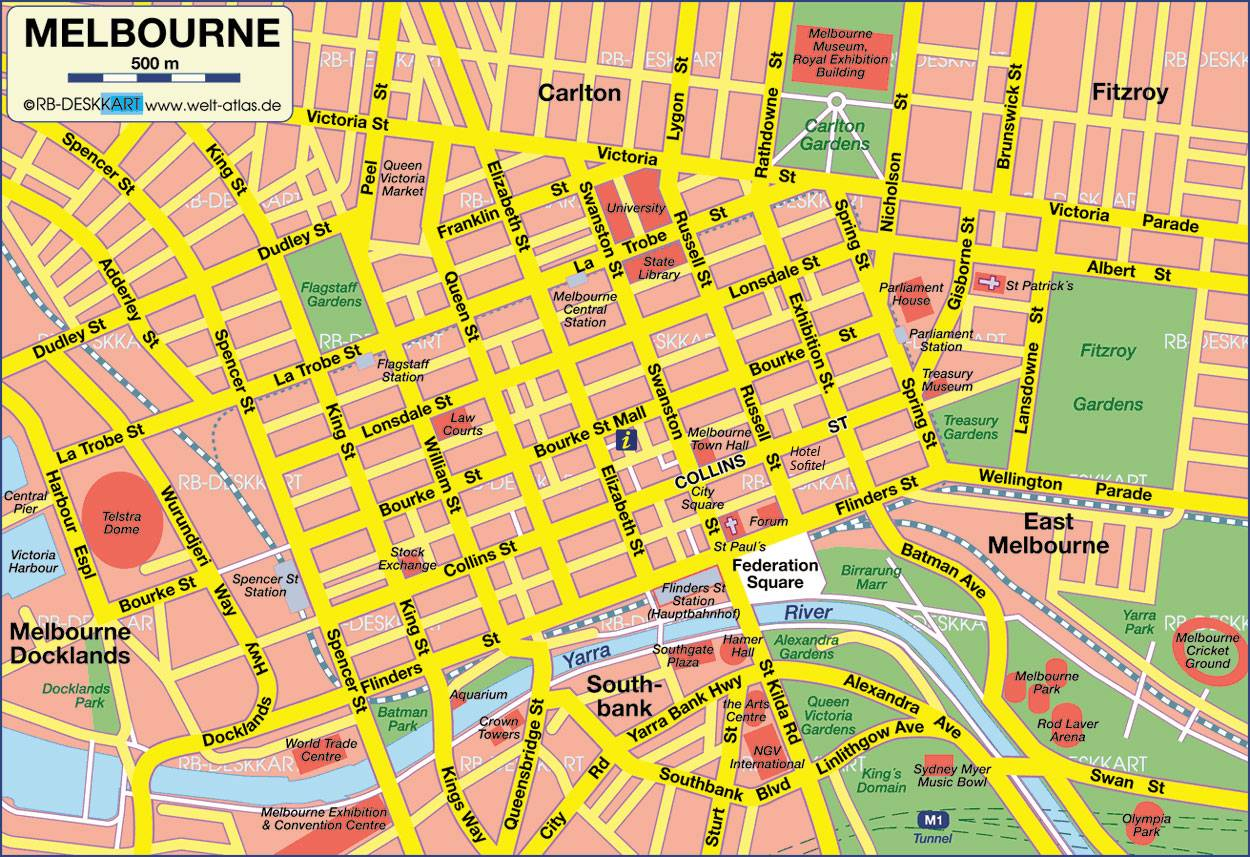
\includegraphics[width=\linewidth,keepaspectratio]{images/cbdmap.jpg}
\end{figure}
\label{sec:Experiments}
The core system was tested by software simulation in various scenarios. Details on the simulation set-up and parameters can be found in Appendix \ref{apdx:simSetUp}. Three different cases in two separate environments were simulated to give a total of six scenarios. The Environments were as follows:
\subsection{Environments}
\label{sec:Experiments:env}
\subsubsection{City}
	The road network of Melbourne CBD was taken with vehicles spawning at random locations, at random times, driving to a random destinations, then going off-line. Lifespans of individual vehicles were short, however the network is always densely populated with new vehicles appearing as old ones go offline.	Meant to simulate the situation of traffic in a busy city centre. See Fig.. \ref{fig:CBDRoads}	
\subsubsection{Highway}
	A flow of a fixed number of vehicles was simulated to run on a fixed route, mostly comprised of straight multi-lane roads. All nodes had larger lifespans than before. By means of overtaking and other reasons, the order of initialisation was not maintained as the order in which the nodes continued to travel. It was meant to simulate the situation of vehicles moving on a highway for a flow of vehicles from a point to a distant point.
\subsection{Situations}
\label{sec:Experiments:sit}
Different situations were simulated to analyse the system's performance against various attack vectors of compromising the the systems ability to produce accurate estimates. The behaviour of a regular node was programmed as follows: Overall accuracy of Sent Messages is around 90\%. The node can determine the truthfulness of 60\% messages it receives with an accuracy of 95\%. %TODO: add citation?.
Further details of a regular node's behaviour can be  found in appendix \ref{apdx:simSetUp}.
\subsubsection{Situation 0}
\label{sec:Experiments:sit:0}
The first situation considered was that of a few (10\%) malicious nodes that send false information on the network with an accuracy of 5\%. The rest of the parameters controlling their behaviour was the same as regular nodes. This situation enables us to analyse the system's performance at detecting false messages and malicious nodes in a scenario where no node is sharing falsified feedback to jeopardise the reputation system. This can then be compared with other situations to spot degradation in performance.
\subsubsection{Situation 1}
\label{sec:Experiments:sit1}
In the second situation, over and above the factors present in situation 0, 10\% Nodes were programmed to send reports with an accuracy of 5\% i.e 95\% reports generated by them are falsified and they send reports on 100\% messages they receive as opposed to 60\%, this was implemented to observe the degradation in the accuracy of estimates with false reports being shared by nodes and the ability of the system to detect the nodes sending falsified reports.
\subsubsection{Situation 2}
\label{sec:Experiments:sit2}
In the third and final situation, over and above the factors present in situation 0, 20\% of nodes were programmed to target 5\% of nodes specifically. These colluding nodes would send falsified feedback on every message received from target nodes while sending useful reports otherwise. This was implemented to analyse the systems ability to detect convoluted methods of compromising it's ability of estimating accuracy where a large percent of malicious nodes send mostly useful feedback in order to not get blacklisted but target specific nodes, either regular or malicious, to alter their primary score.
\subsection{Scenarios}
The various permutations of environments and situations were termed as follows.
\begin{itemize}
	\item[-] Scenario 0: Situation 0 in City
	\item[-] Scenario 1: Situation 1 in City
	\item[-] Scenario 2: Situation 2 in City
	\item[-] Scenario 10: Situation 0 on Highway
	\item[-] Scenario 11: Situation 1 on Highway
	\item[-] Scenario 12: Situation 2 on Highway
\end{itemize}
\section{Results}
\label{sec:Results}
\begin{figure}[!t]
	\caption{Absolute error (difference between actual accuracy of node and estimated accuracy) vs. Percentage of nodes for which there was less than 'x'\% error in Scenario 0 (above) and Scenario 1 (below)}
	\label{fig:plot:comparitiveSCN0&1}
	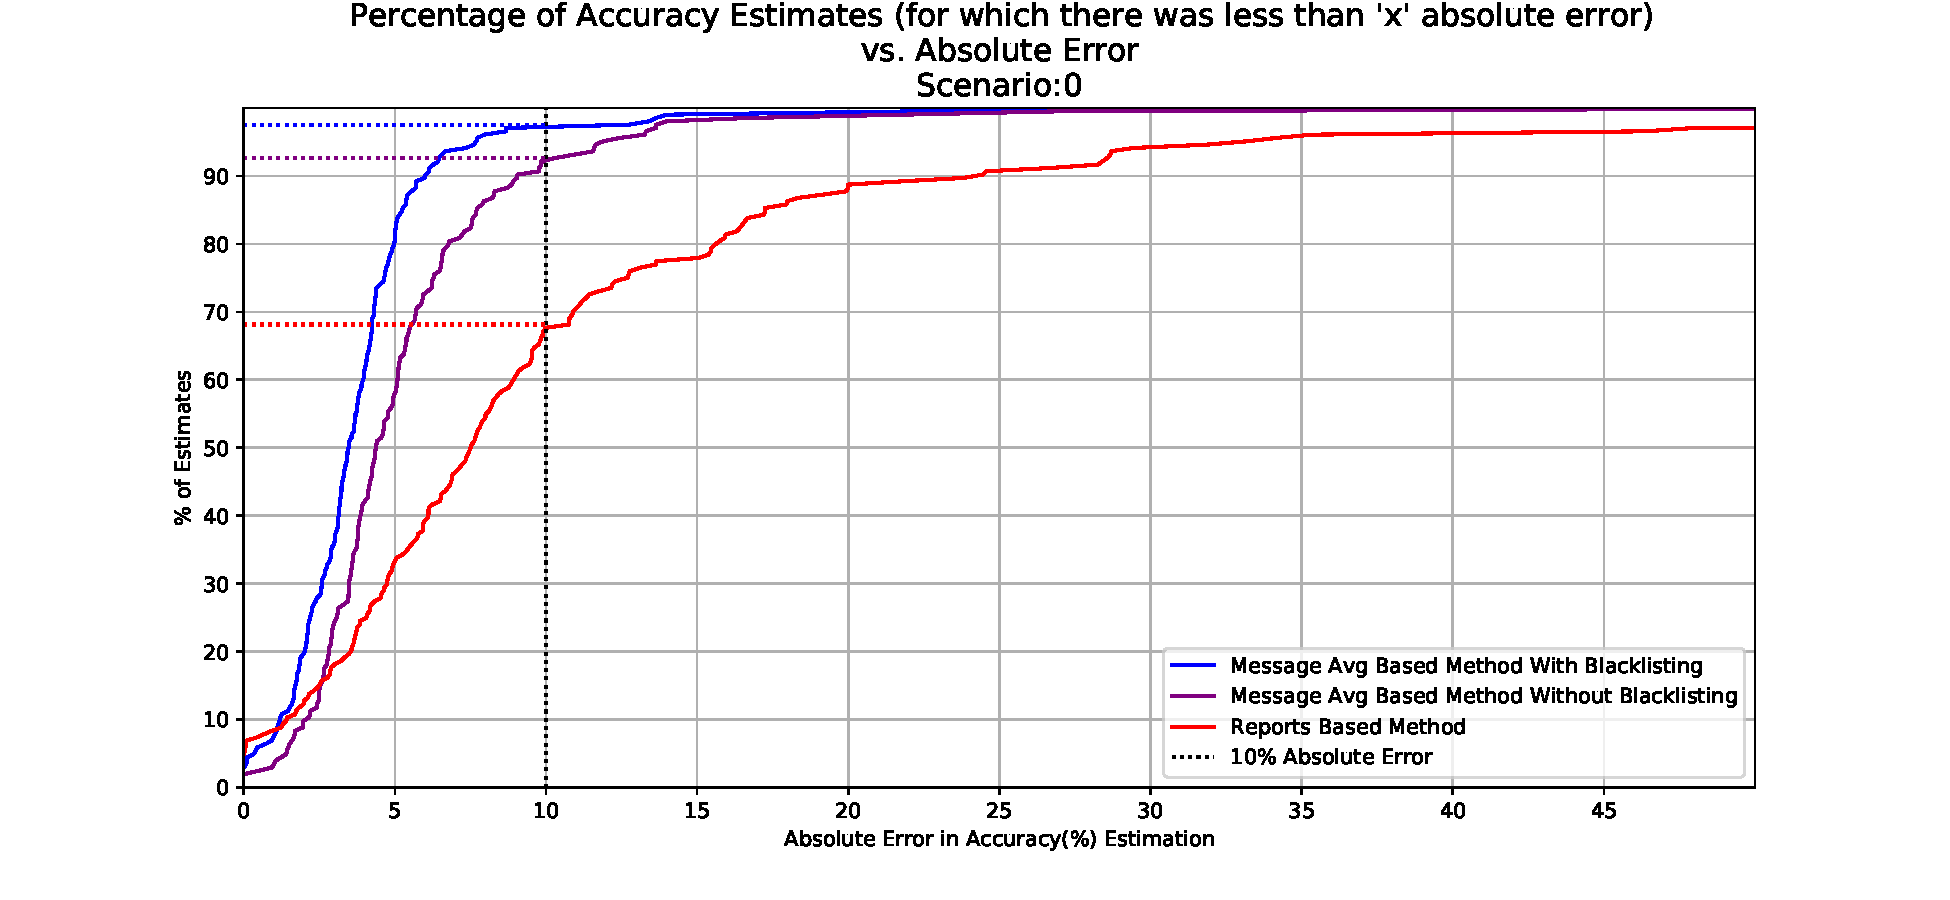
\includegraphics[width=0.5\textwidth, trim={80 20 80 30},clip]{images/SCN0_AbsoluteErrorsInEstimationComparison.pdf}
	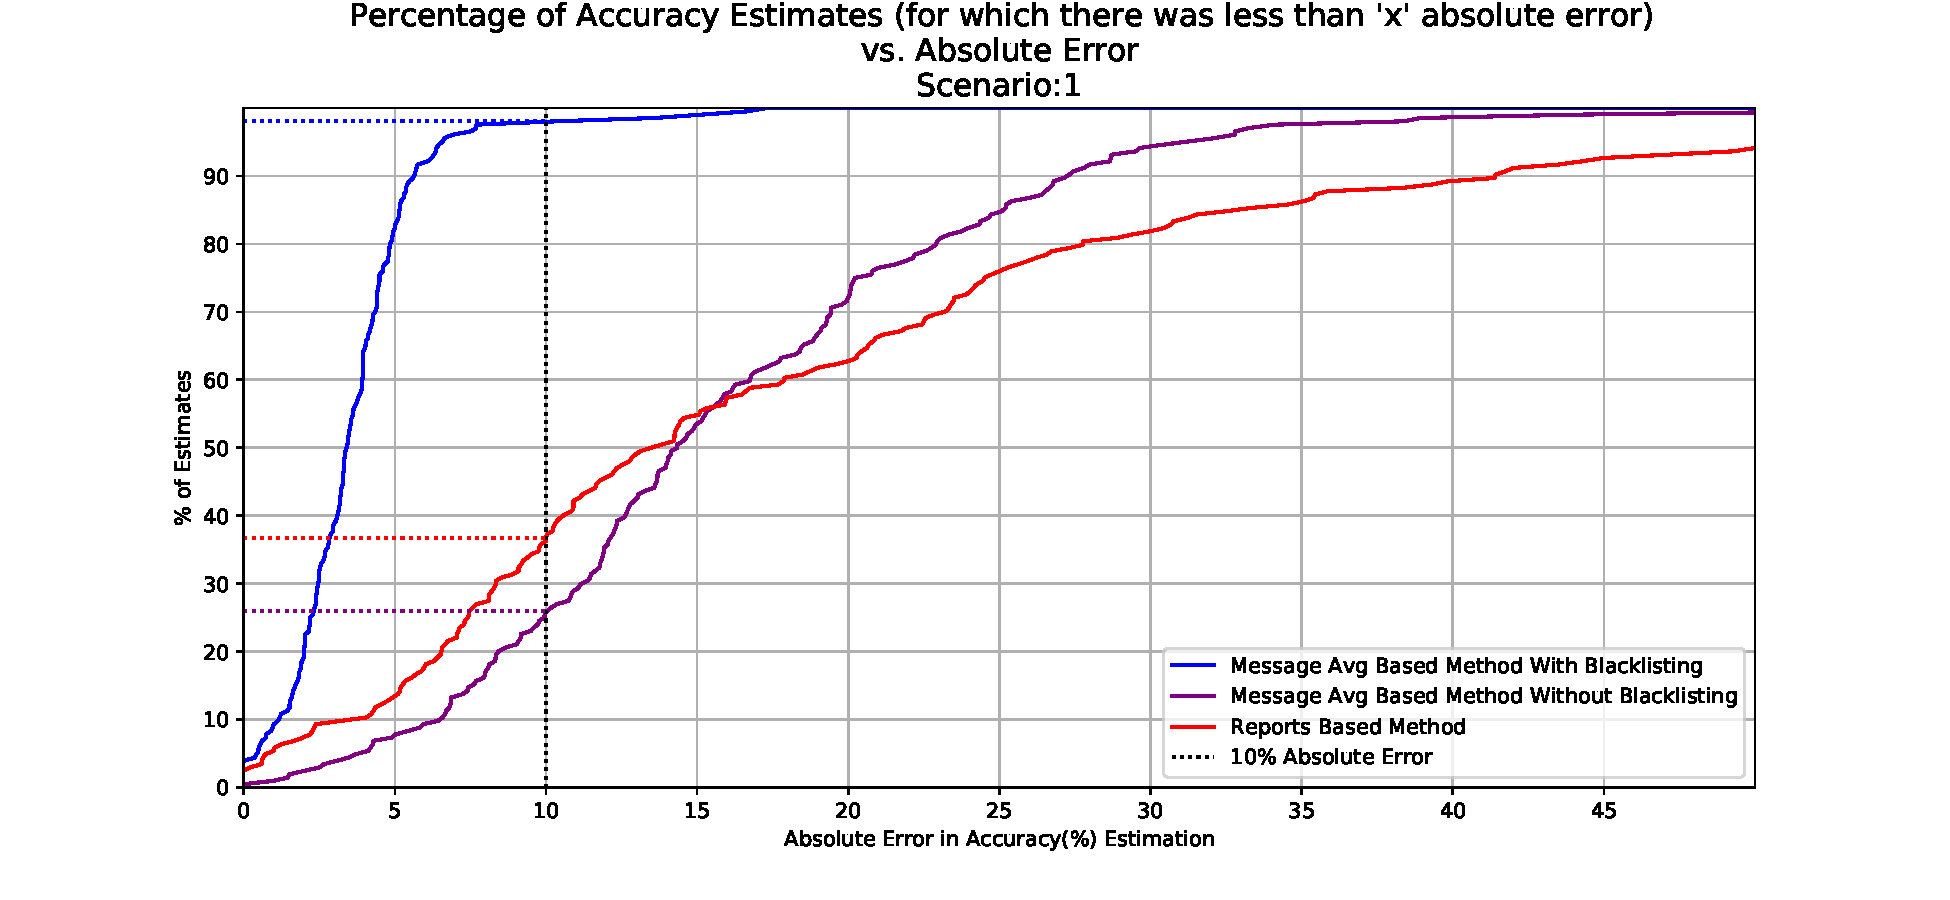
\includegraphics[width=0.5\textwidth, trim={80 20 80 30},clip]{images/SCN1_AbsoluteErrorsInEstimationComparison.pdf}
\end{figure}
\begin{figure}[!t]
	\caption{Mean Secondary Score vs. Accuracy of Reports Sent, Scatter plot for Scenario 1}
	\label{fig:plot:ssSCN1}
	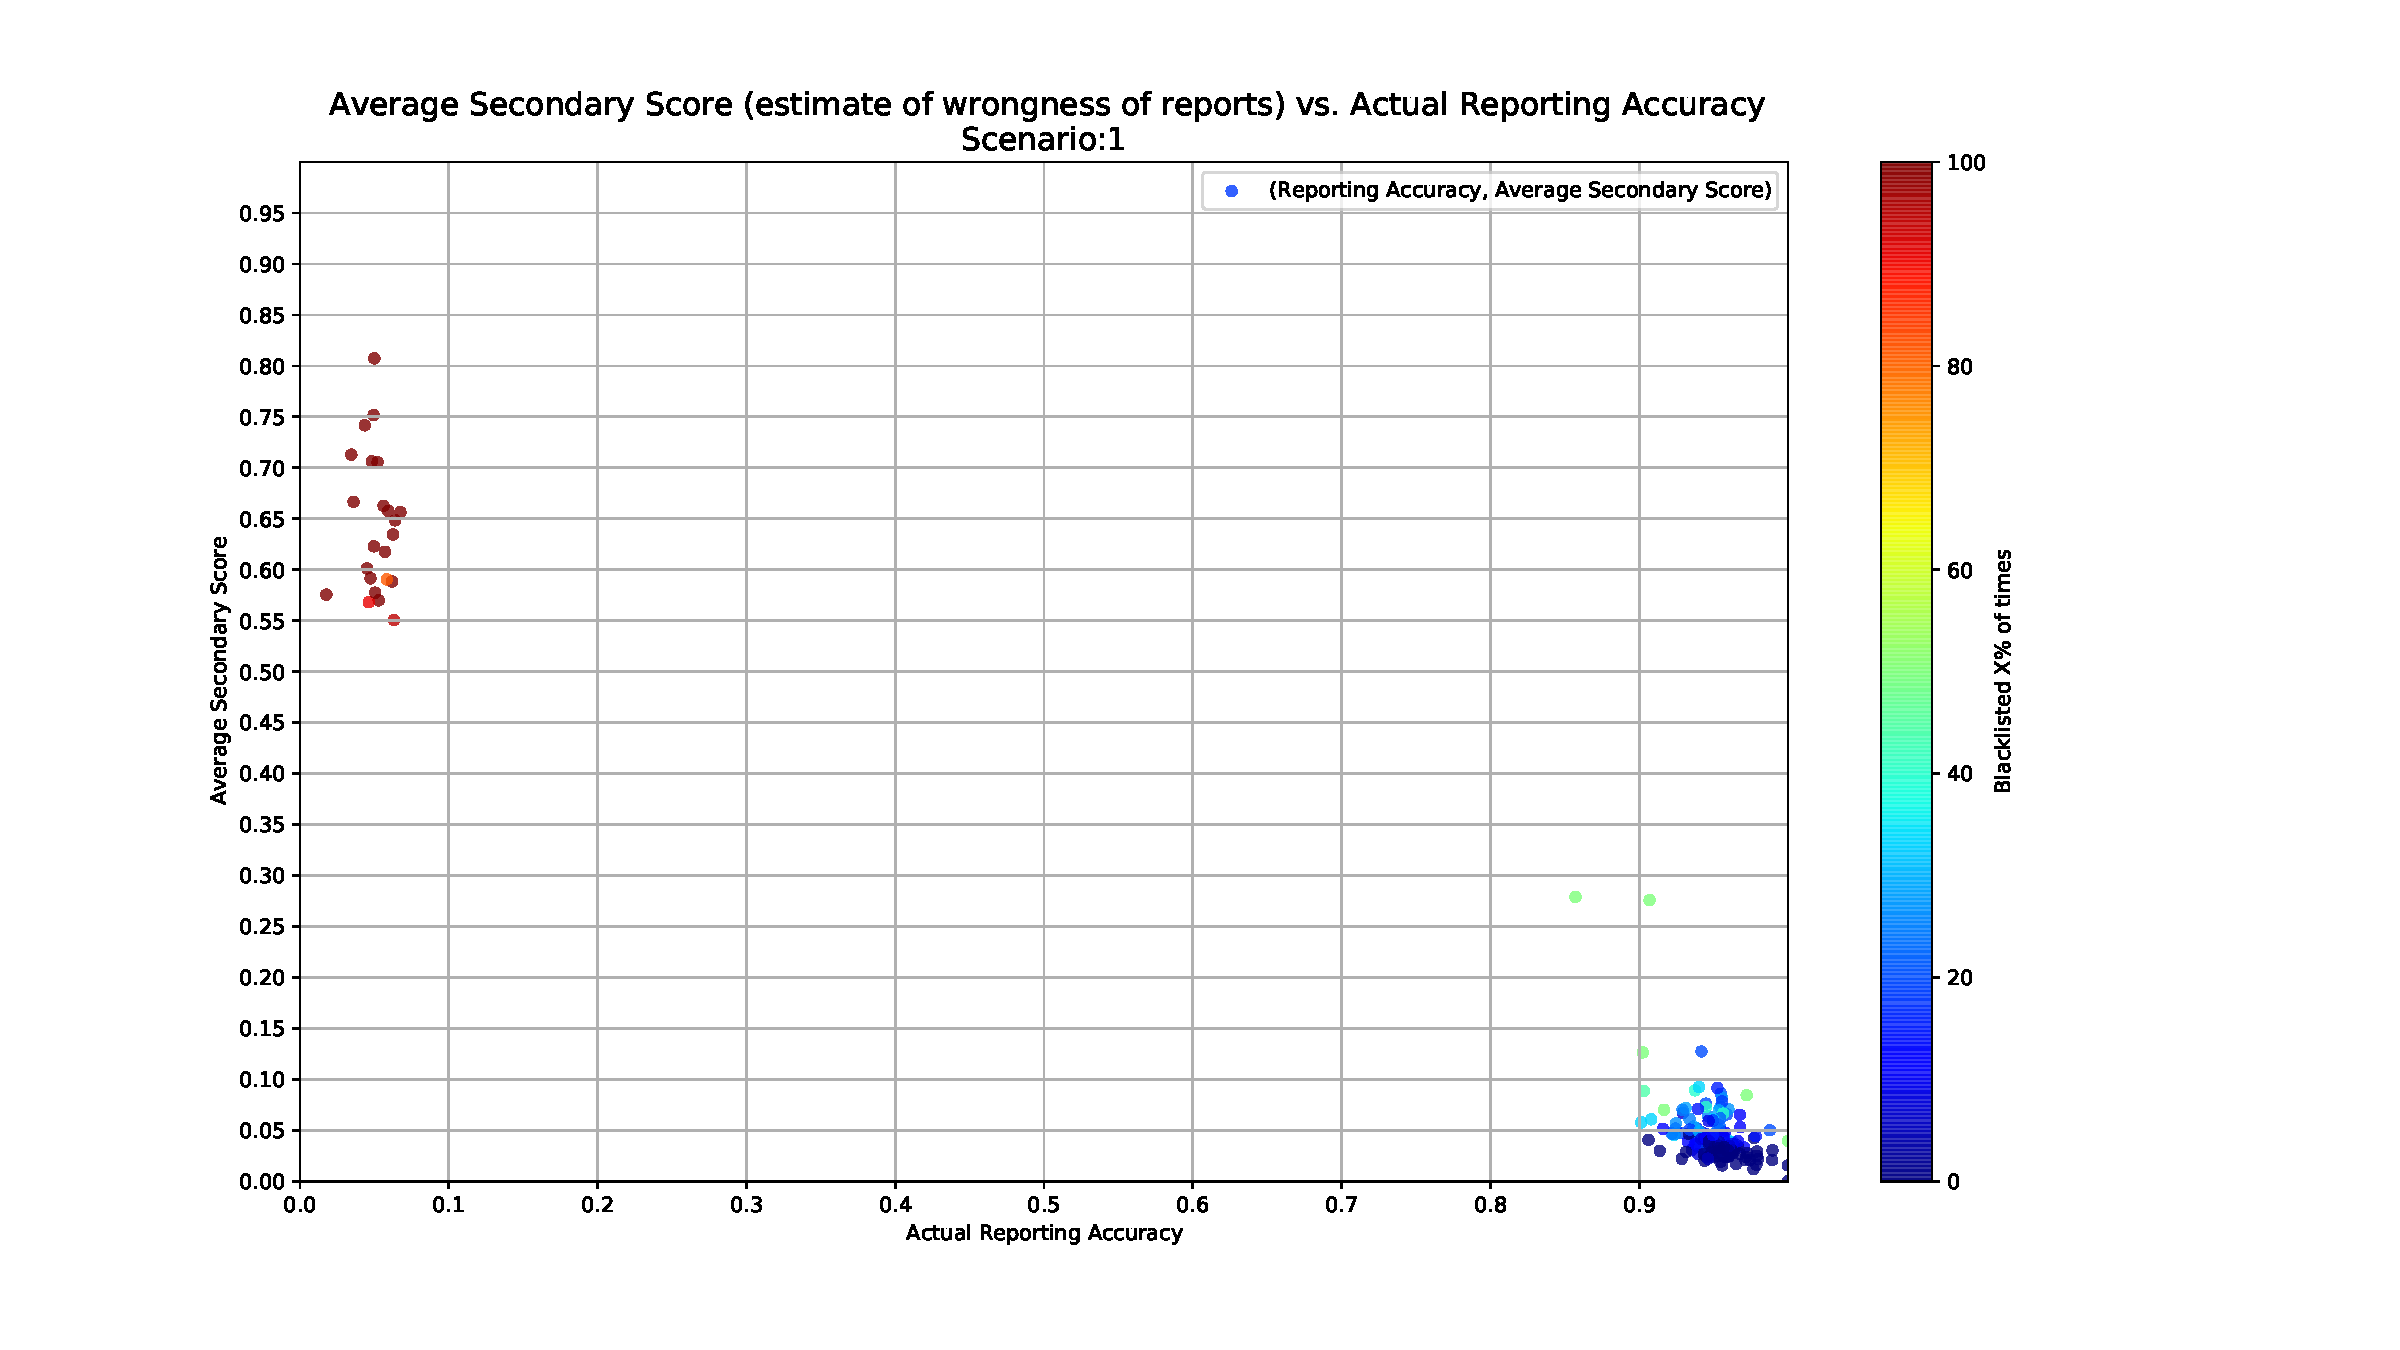
\includegraphics[width=0.5\textwidth, trim={100 50 185 72},clip]{images/SCN1_ReportingAccuracy_Vs_AvgSecondaryScore.pdf}
\end{figure}
\begin{figure}[!t]
	\caption{Mean Secondary Score vs. Accuracy of Reports Sent, Scatter plot for Scenario 2}
	\label{fig:plot:ssSCN2}
	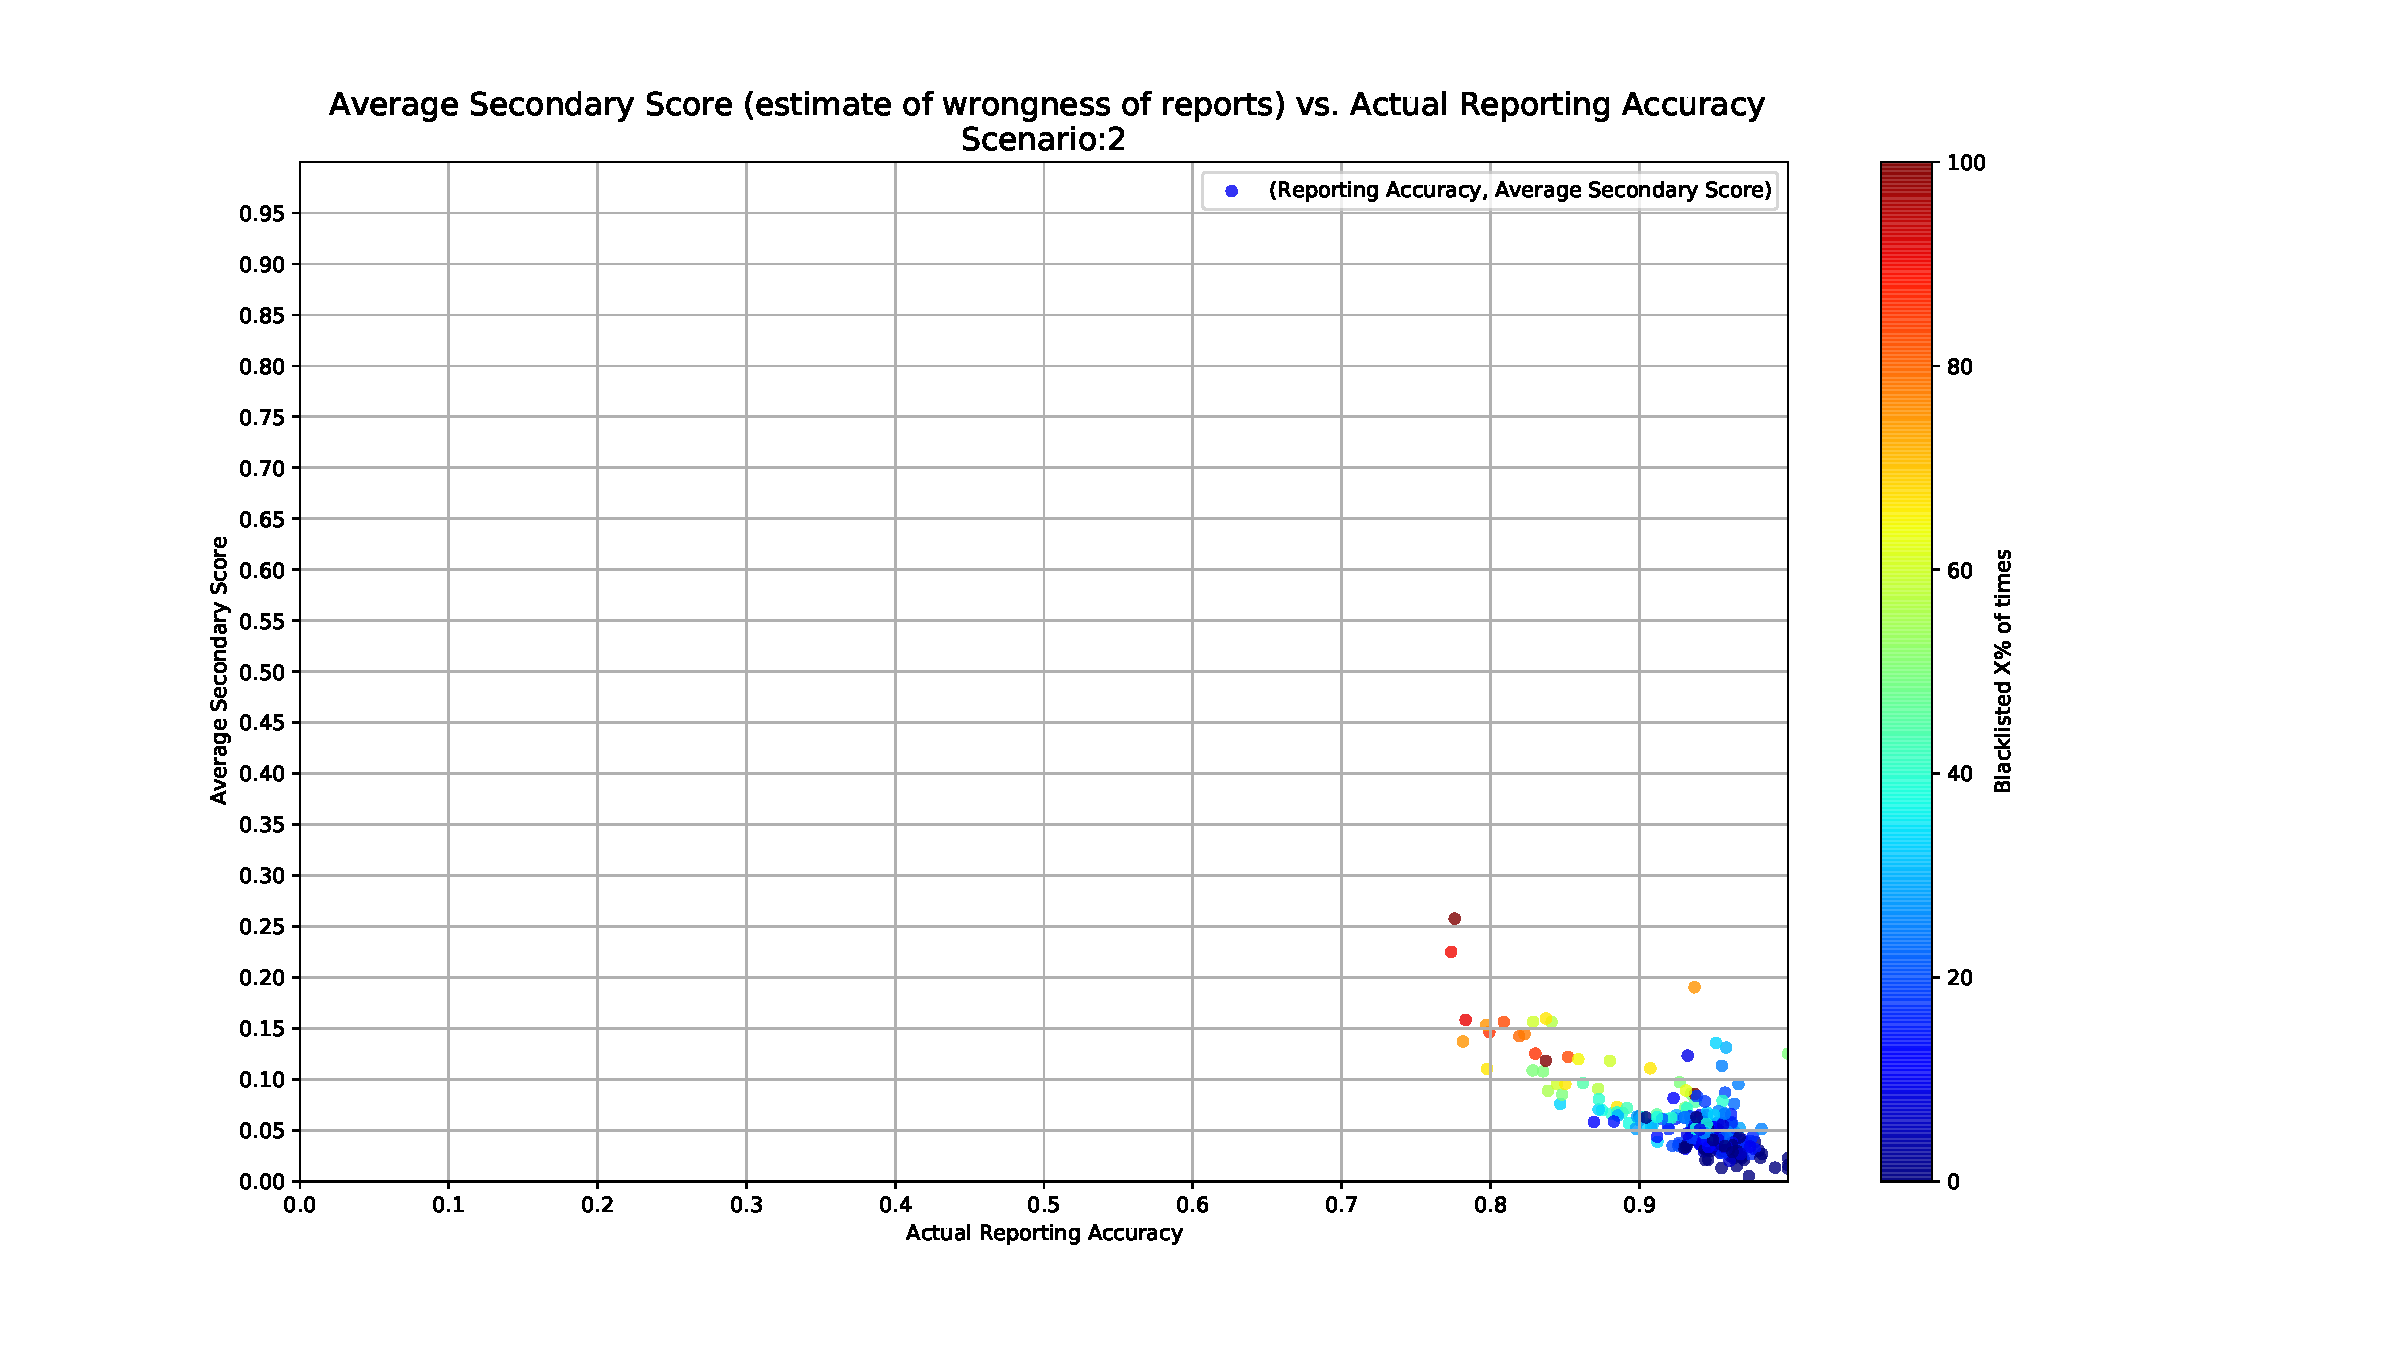
\includegraphics[width=0.5\textwidth, trim={100 50 185 72},clip]{images/SCN2_ReportingAccuracy_Vs_AvgSecondaryScore.pdf}
\end{figure}
\begin{figure}[!t]
	\caption{Primary Score vs. Actual Accuracy - Scatter plot for Scenario 12. Without blacklisting (above) and with blacklisting (below).}
	\label{fig:plot:psscatterSCN12}
	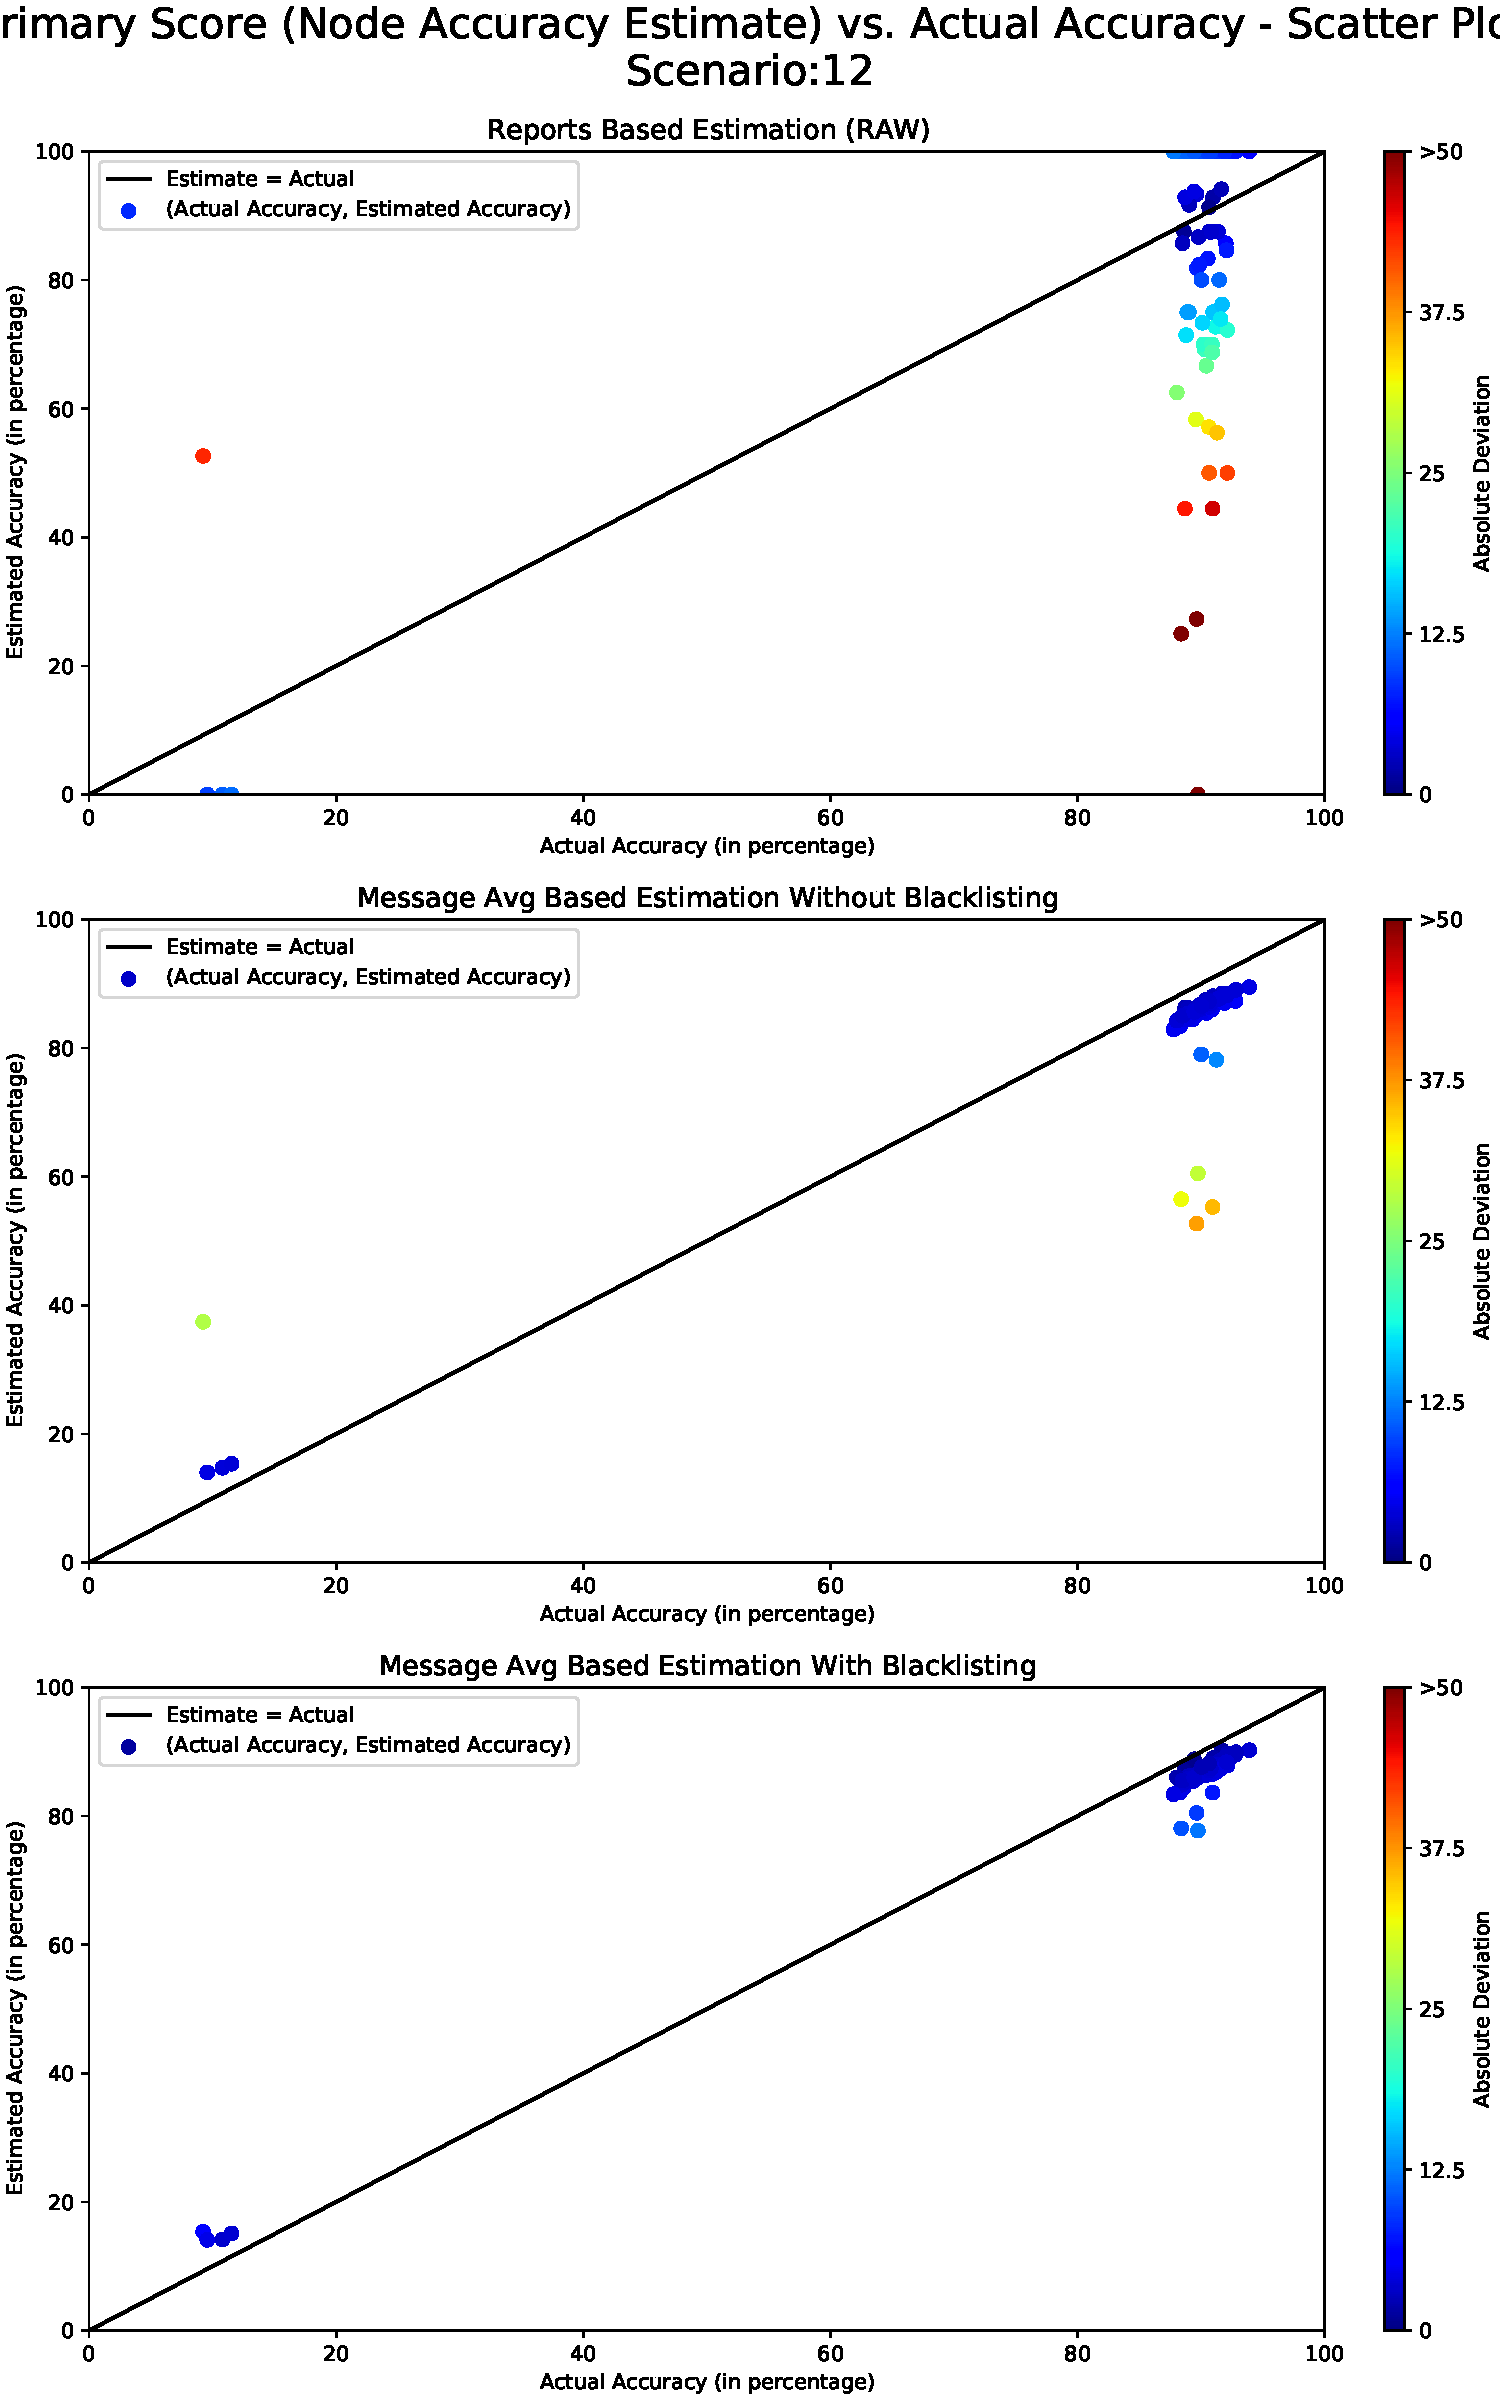
\includegraphics[width=\linewidth, trim={0 5 15 420}, clip]{images/SCN12_PrimaryScoreVsActualAccuracyComparitive.pdf}
\end{figure}
Various plots on the results of the simulations for each scenario are presented in Appendix. \ref{apdx:simResults}. It can be observed from the results that in the absence of falsified reports, the system can estimate the accuracy of almost all (~97\%) nodes in city environment and all nodes in highway environment with less than 10 absolute error where accuracy and scores were measured in percentage.\\
Comparing the system's performance between scenario 0 and scenario 1 (where falsified reports were being sent) shows that significant percentage of scores are highly inaccurate for scores calculated without blacklisting. In scenario 0, 92.2\% of accuracy estimates without blacklisting had less then 10 absolute error (0.1 when normalised) where accuracy and scores were measured in percentage. In scenario 1 this dropped down to 25.5\% of estimates. Whereas the same measure for score calculation with blacklisting remained about the same. This can be seen in Fig. \ref{fig:plot:comparitiveSCN0&1}. Similar observations can be made when comparing scenario 10 and 11. This lack of degradation of the system can be attributed to it's ability to accurately identify nodes that send false feedback all the time. This can be seen in Fig. \ref{fig:plot:ssSCN1}, where nodes with low utility of reports were almost always blacklisted as indicated by the deep red colour.\\
In Scenarios 2 and 12, where a more intelligent approach to sabotage the system's accuracy estimate (score) of a node was made by 20\% nodes in the network that acted like regular nodes except when sending reports on 5\% nodes that were the targets for the collusion, the accuracy of those target nodes was highly inaccurate as expected, this can be seen in Fig. \ref{fig:plot:psscatterSCN12} (lower) where the accuracy of 5 nodes was uniquely inaccurate. With blacklisting, however, the errors were minimal as can be observed in Fig. \ref{fig:plot:psscatterSCN12} (upper). This lack of error can again be attributed to the system's ability to accurately identify and blacklist nodes that send false feedback even some of the times. This can be observed from in Fig. \ref{fig:plot:ssSCN2} where nodes with slightly lower utility of reports blacklisted sometimes to most often as indicated by the light blue to red colours. It is important to note that the special collusion detection methods of multimodality detection\cite{c:DipTest}\cite{c:SilvermansTest} as explained in section \ref{sec:PM:usage} was not leveraged during experiments.

\section{Conclusion}
\label{sec:Conclusion}
In this paper we proposed a primarily centralised reputation mechanism that relies on feedback generated by nodes using false information detection mechanisms to first evaluate the truth value for each message, after filtering out the false/malicious feedback using rudimentary statistical methods. Then, using these truth values, for messages the reputation score was calculated. We further proposed possible extensions of this method such as specialised method for detection of collusion, and various ways in which this data can be shared by the RSUs to the rest of the network. We also proposed the ways in which the nodes can utilise this data to generate reputation scores for nodes at their end and to dynamically alter this score in between RSU broadcasts. The core method for reputation score calculation was tested using software simulation where it was observed that the system was highly accurate at estimating the accuracy of nodes (reputation) when the feedback was entirely genuine. The estimates naturally became much more inaccurate with falsified feedback from ten percent of the network however this change in error was almost entirely eliminated with the proposed method for false feedback filtration. The same observations were made in a scenario where a large group of attackers maintained a good ratio of useful to false feedback by colluding to targeting specific few nodes.

% if have a single appendix:
%\appendix[Proof of the Zonklar Equations]
% or
%\appendix  % for no appendix heading
% do not use \section anymore after \appendix, only \section*
% is possibly needed

% use appendices with more than one appendix
% then use \section to start each appendix
% you must declare a \section before using any
% \subsection or using \label (\appendices by itself
% starts a section numbered zero.)
%

\appendices
\setcounter{figure}{0}
\renewcommand\thefigure{\Alph{section}.\arabic{figure}}
\section{Simulation Set-Up}
\label{apdx:simSetUp}
\subsection{Traffic Simulation}
Traffic was simulated on SUMO. For city environment the road network of Melbourne CBD was generated using the osm web wizard script. Vehicle trips for this road network were created by a call to the random trips script from within the osm web wizard script. Routes for the generated random passenger trips were calculated with explicitly calling the duarouter method of SUMO. For the Highway Scenario, road network of larger Melbourne area was generated using the osm web wizard script. After this two points on the network, one in front of Deakin University, Burwood, and one in Fitzroy were chosen as starting and ending points. A route for the same was calculated using Duarouter and a flow of 50/100 vehicles was generated on that route.
\subsection{Network/Application Simulation}
Veins on OMNET++ was utilised to simulate the network and the application. The default parameters in veins for antenna strength were utilised which are based on \cite{c:AntennaOmnetpp}, same applies to 11p parameters and so on.
\subsection{Regular Nodes }
\begin{itemize}
	\item Overall accuracy of Sent Messages is around 90\%.
	\item Can determine the truthfulness of 60\% messages it receives with an accuracy of 95\%.
	\item Sends a message on a network every 4s$ \pm $ 2000ms.
	\item Sends a report (its evaluation of a received message, if evaluated) in 2s$ \pm $ 1000ms
	\item Sends a request on the network for all nodes to send their evaluations of all messages from a node when a message from a node is encountered for the first time in 1s$ \pm $ 500ms
	\item Can oblige such a request in 1s$ \pm $ 500ms
\end{itemize}
Other nodes' behaviour was different from a regular in only ways previously explained in Section \ref{sec:Experiments} (\ref{sec:Experiments:sit1} and \ref{sec:Experiments:sit2}).

\section{Simulation Results}
\label{apdx:simResults}

The the performance of the system in Situations 0 (Scenario 0 \& 10), 1 (Scenario 1 \& 11) and 2 (Scenario 2 \& 12) is visualised in Figures  \ref{fig:apdx:ev0}, \ref{fig:apdx:ev1} and \ref{fig:apdx:ev2} respectively.
In these figures "Message Average Based Estimation with Blacklisting" refers to the proposed system, "Message Average Based Estimation without Blacklisting" refers to score calculation without blacklisting and "Reports Based Estimation" refers to the RAW Score (See Section \ref{sec:PM:ScoreGeneretion})
\begin{figure*}[!ht]
	\caption{Graphs for Results of Scenario 0 and 10. (a) Primary Score vs. Actual Accuracy - Scatter plot, without (above) and with (below) blacklisting for Scenario 0 (left) and Scenario 10 (right) (b) Absolute error (difference between actual accuracy of node and estimated accuracy) vs. Percentage of nodes for which there was less than 'x'\% error for Scenario 0 (left) and Scenario 10 (right) (c) Mean Secondary Score vs. Accuracy of Reports Sent - Scatter plot for Scenario 0 (left) and Scenario 10 (right)}
	\label{fig:apdx:ev0}
	\centering
	\subfloat[]{
		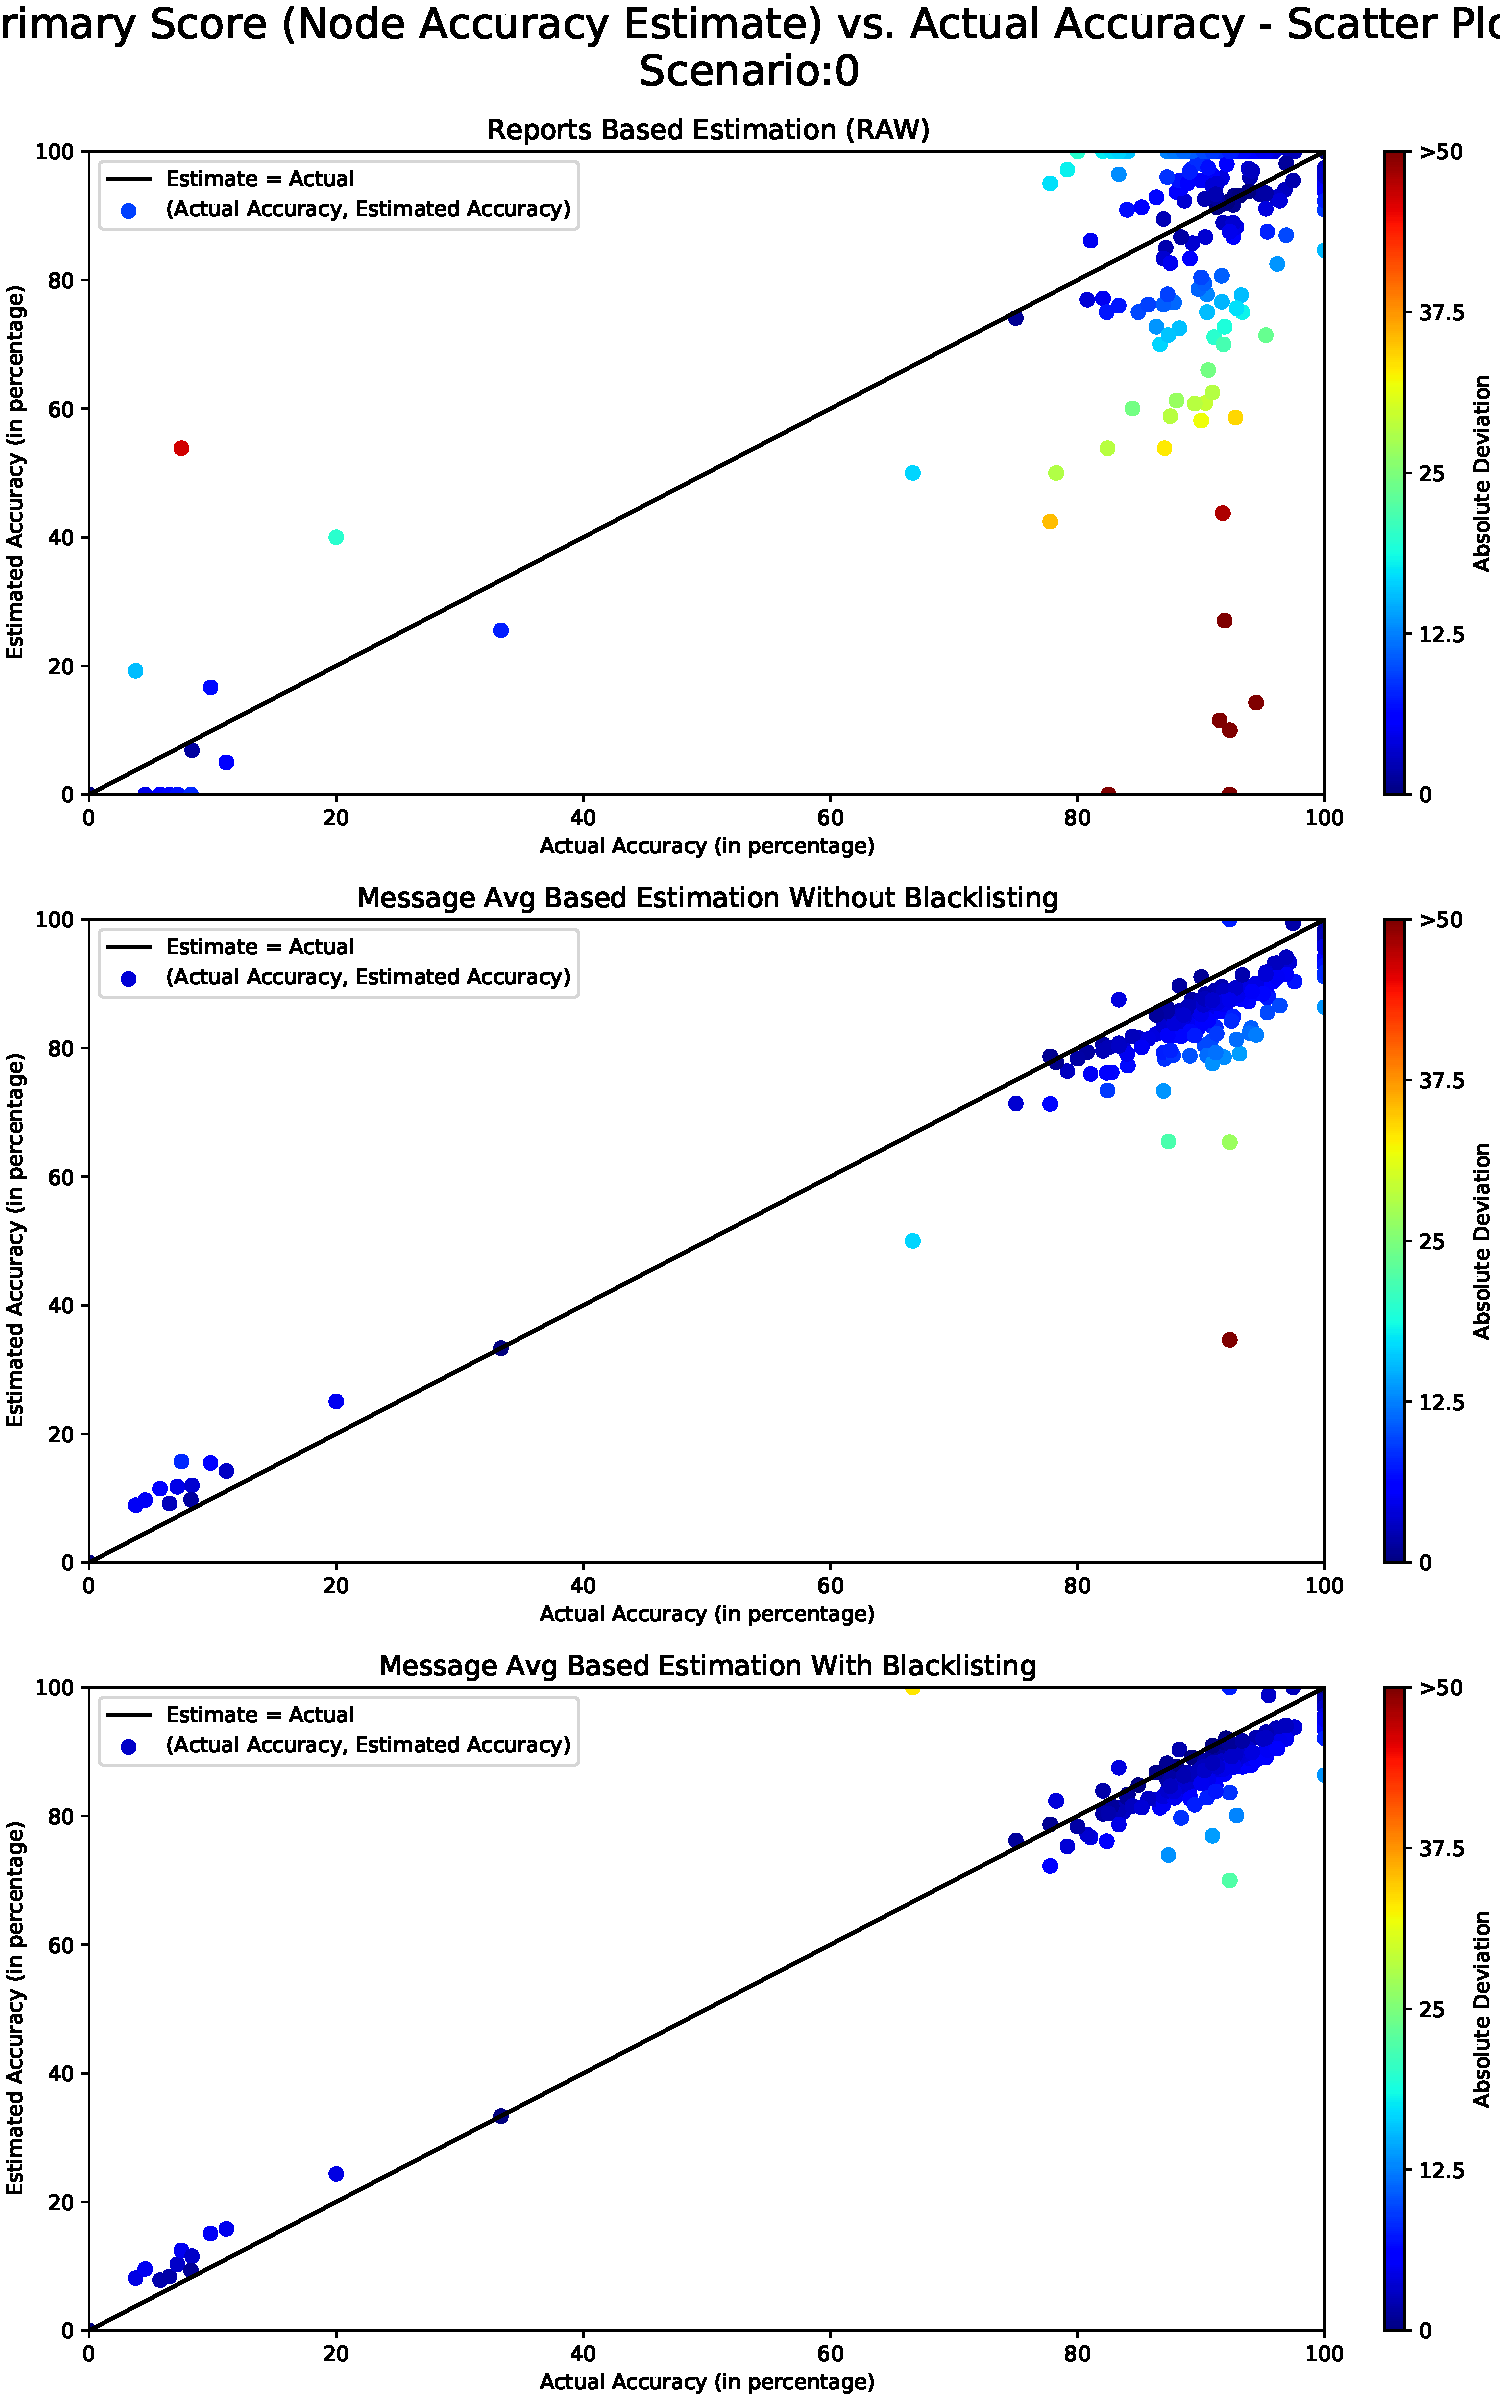
\includegraphics[width=0.5\linewidth, trim={0 5 15 420}, clip]{images/SCN0_PrimaryScoreVsActualAccuracyComparitive.pdf}
		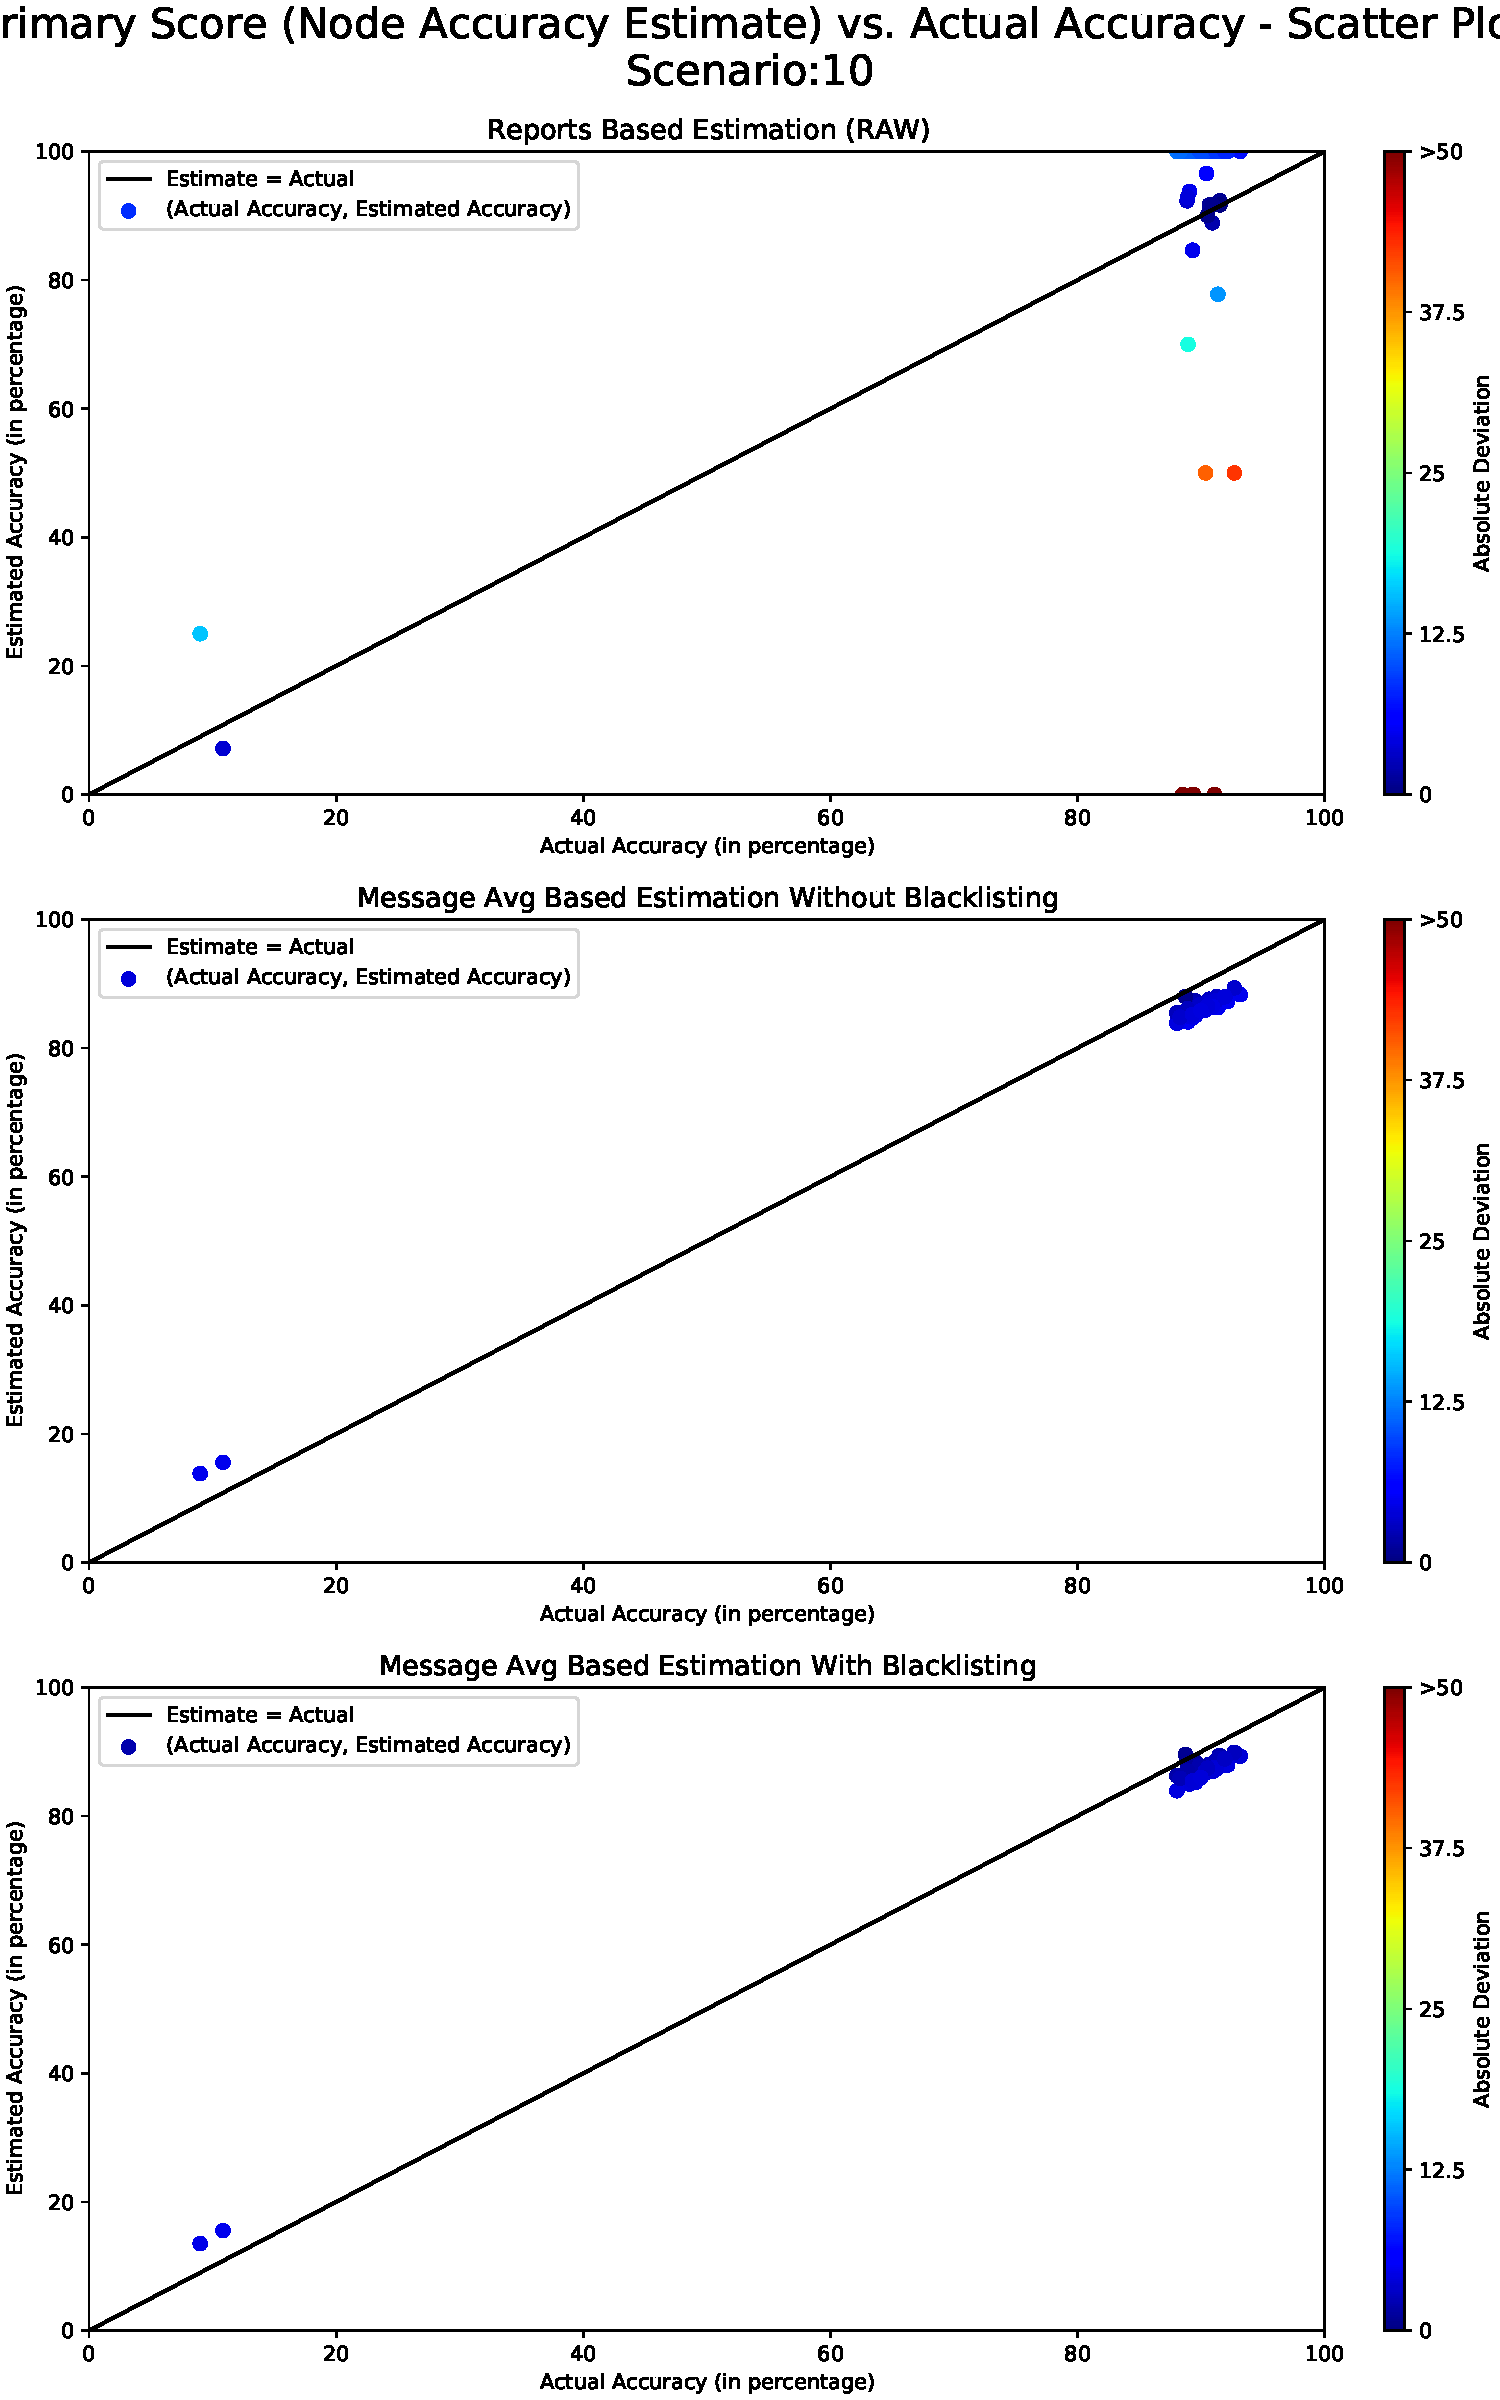
\includegraphics[width=0.5\linewidth, trim={0 5 15 420}, clip]{images/SCN10_PrimaryScoreVsActualAccuracyComparitive.pdf}
	} \\\vfill
	\subfloat[]{
		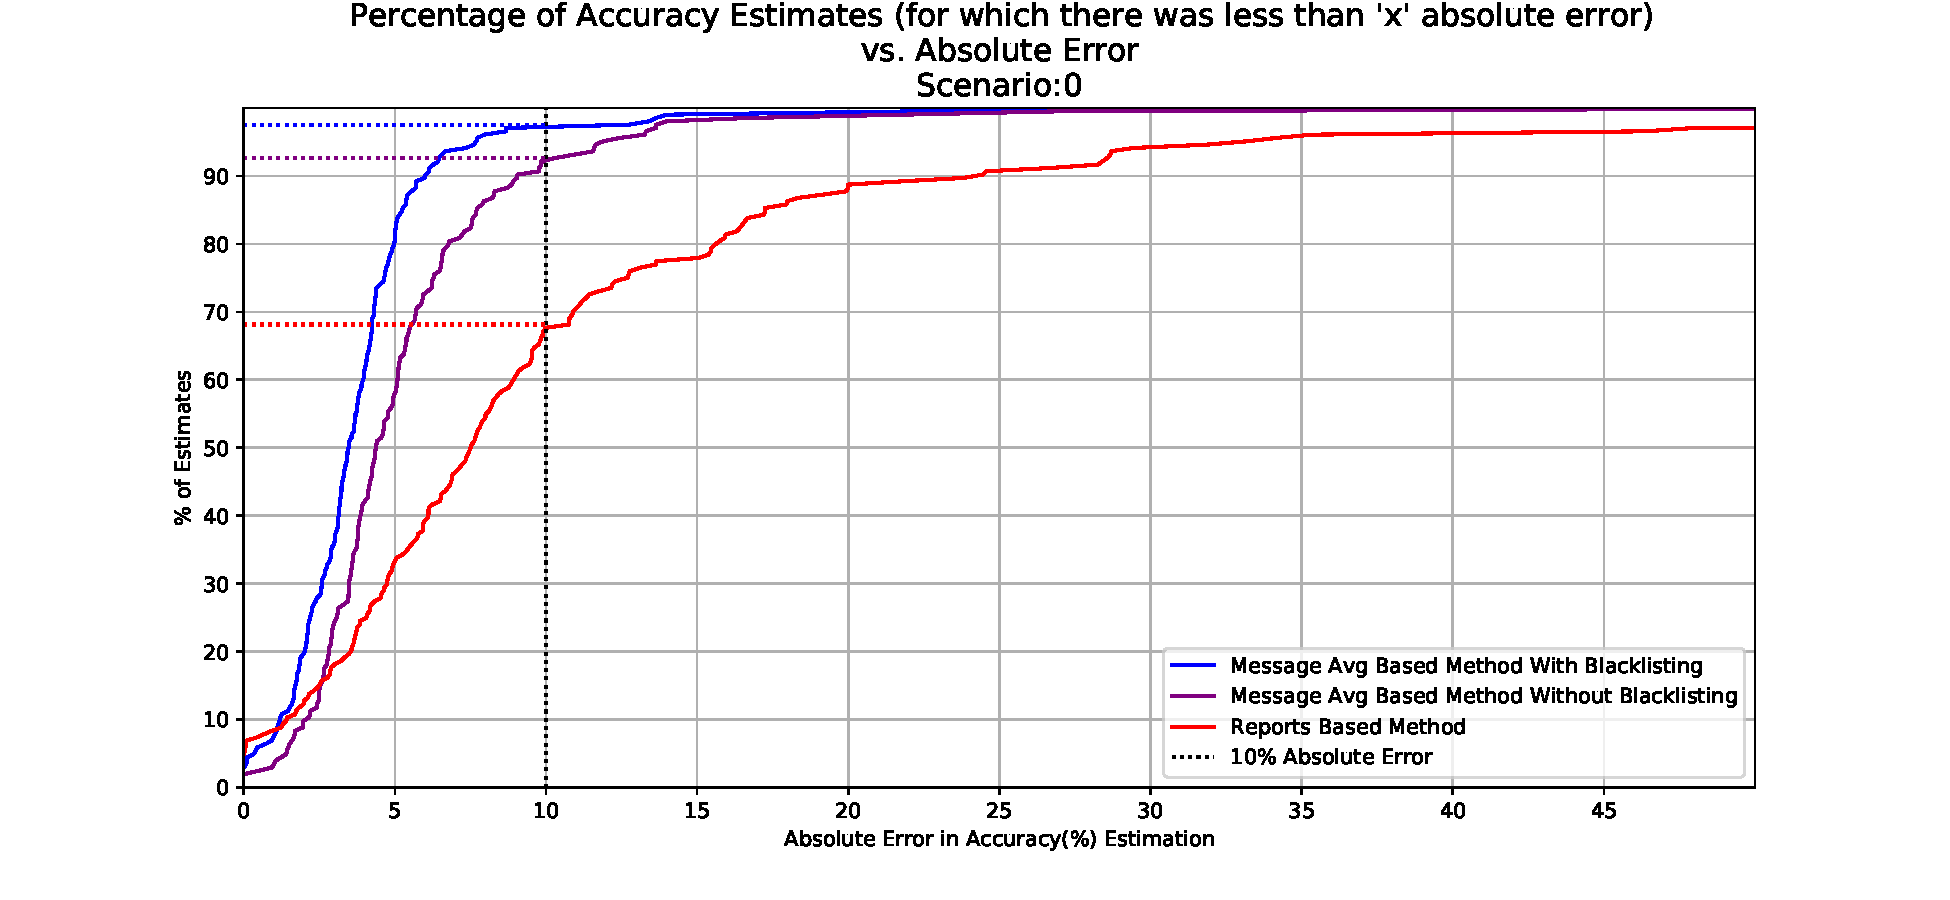
\includegraphics[width=0.5\linewidth, trim={80 25 90 50}, clip]{images/SCN0_AbsoluteErrorsInEstimationComparison.pdf}
		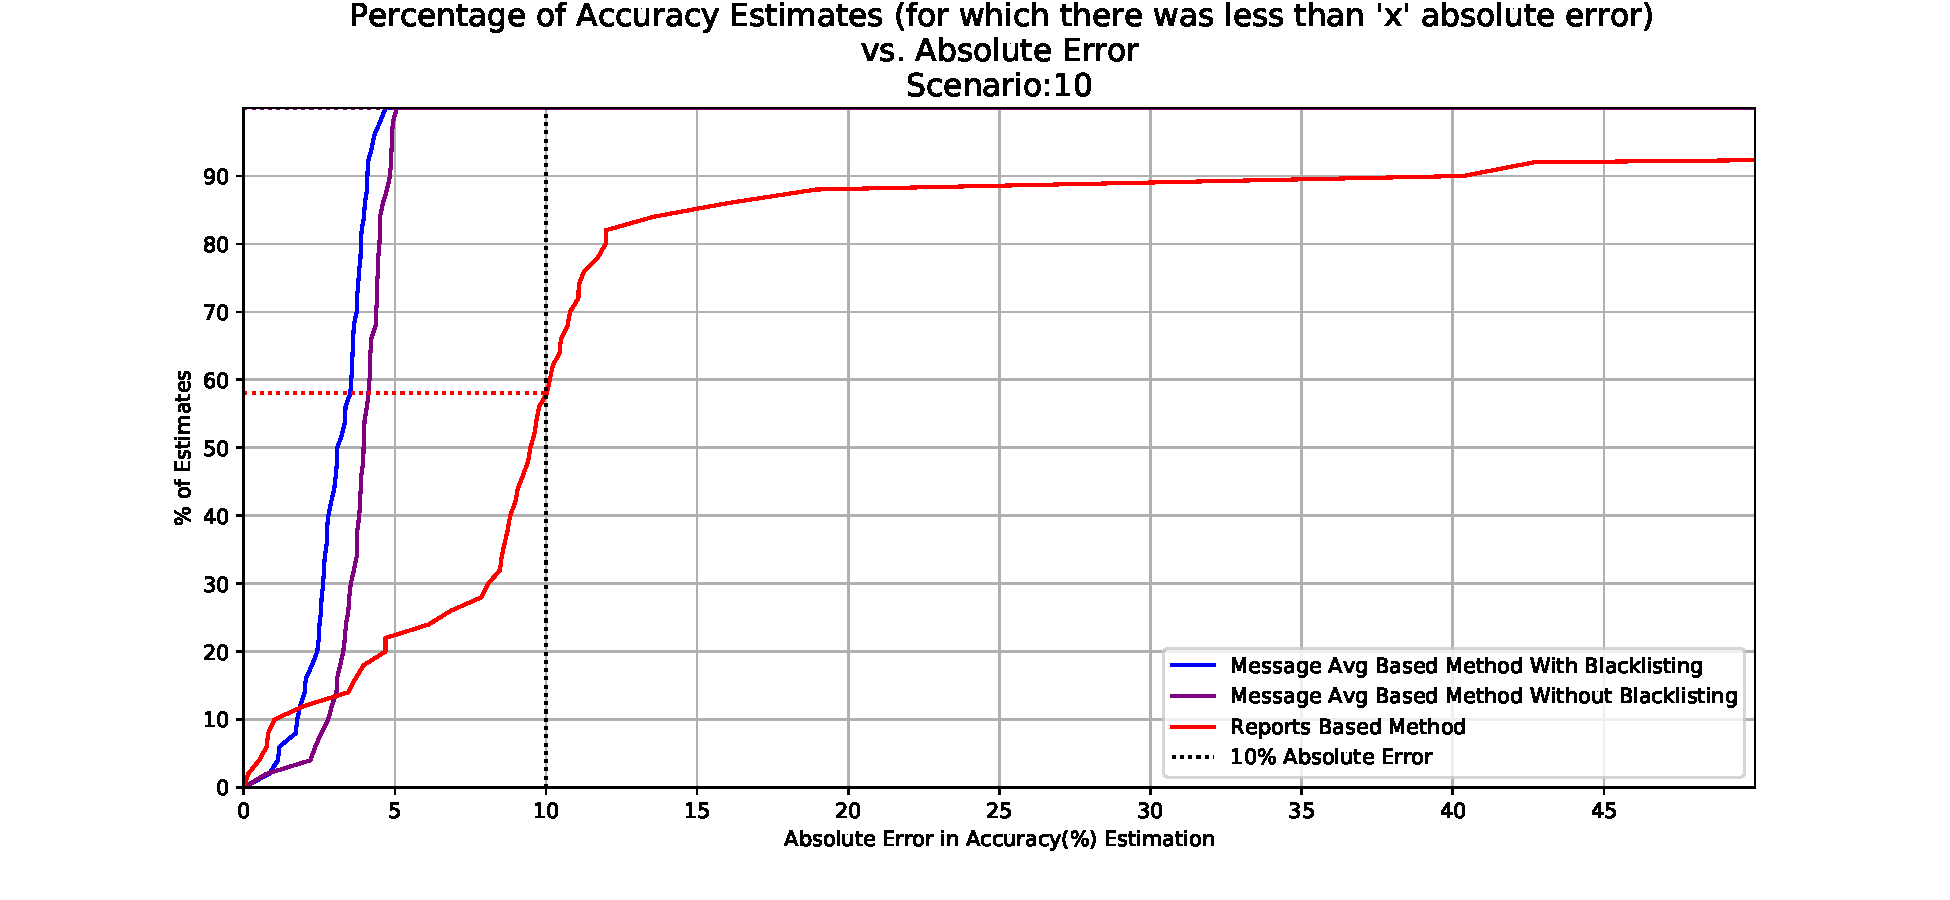
\includegraphics[width=0.5\linewidth, trim={80 25 90 50}, clip]{images/SCN10_AbsoluteErrorsInEstimationComparison.pdf}
	}
	\hfill
	\subfloat[]{
		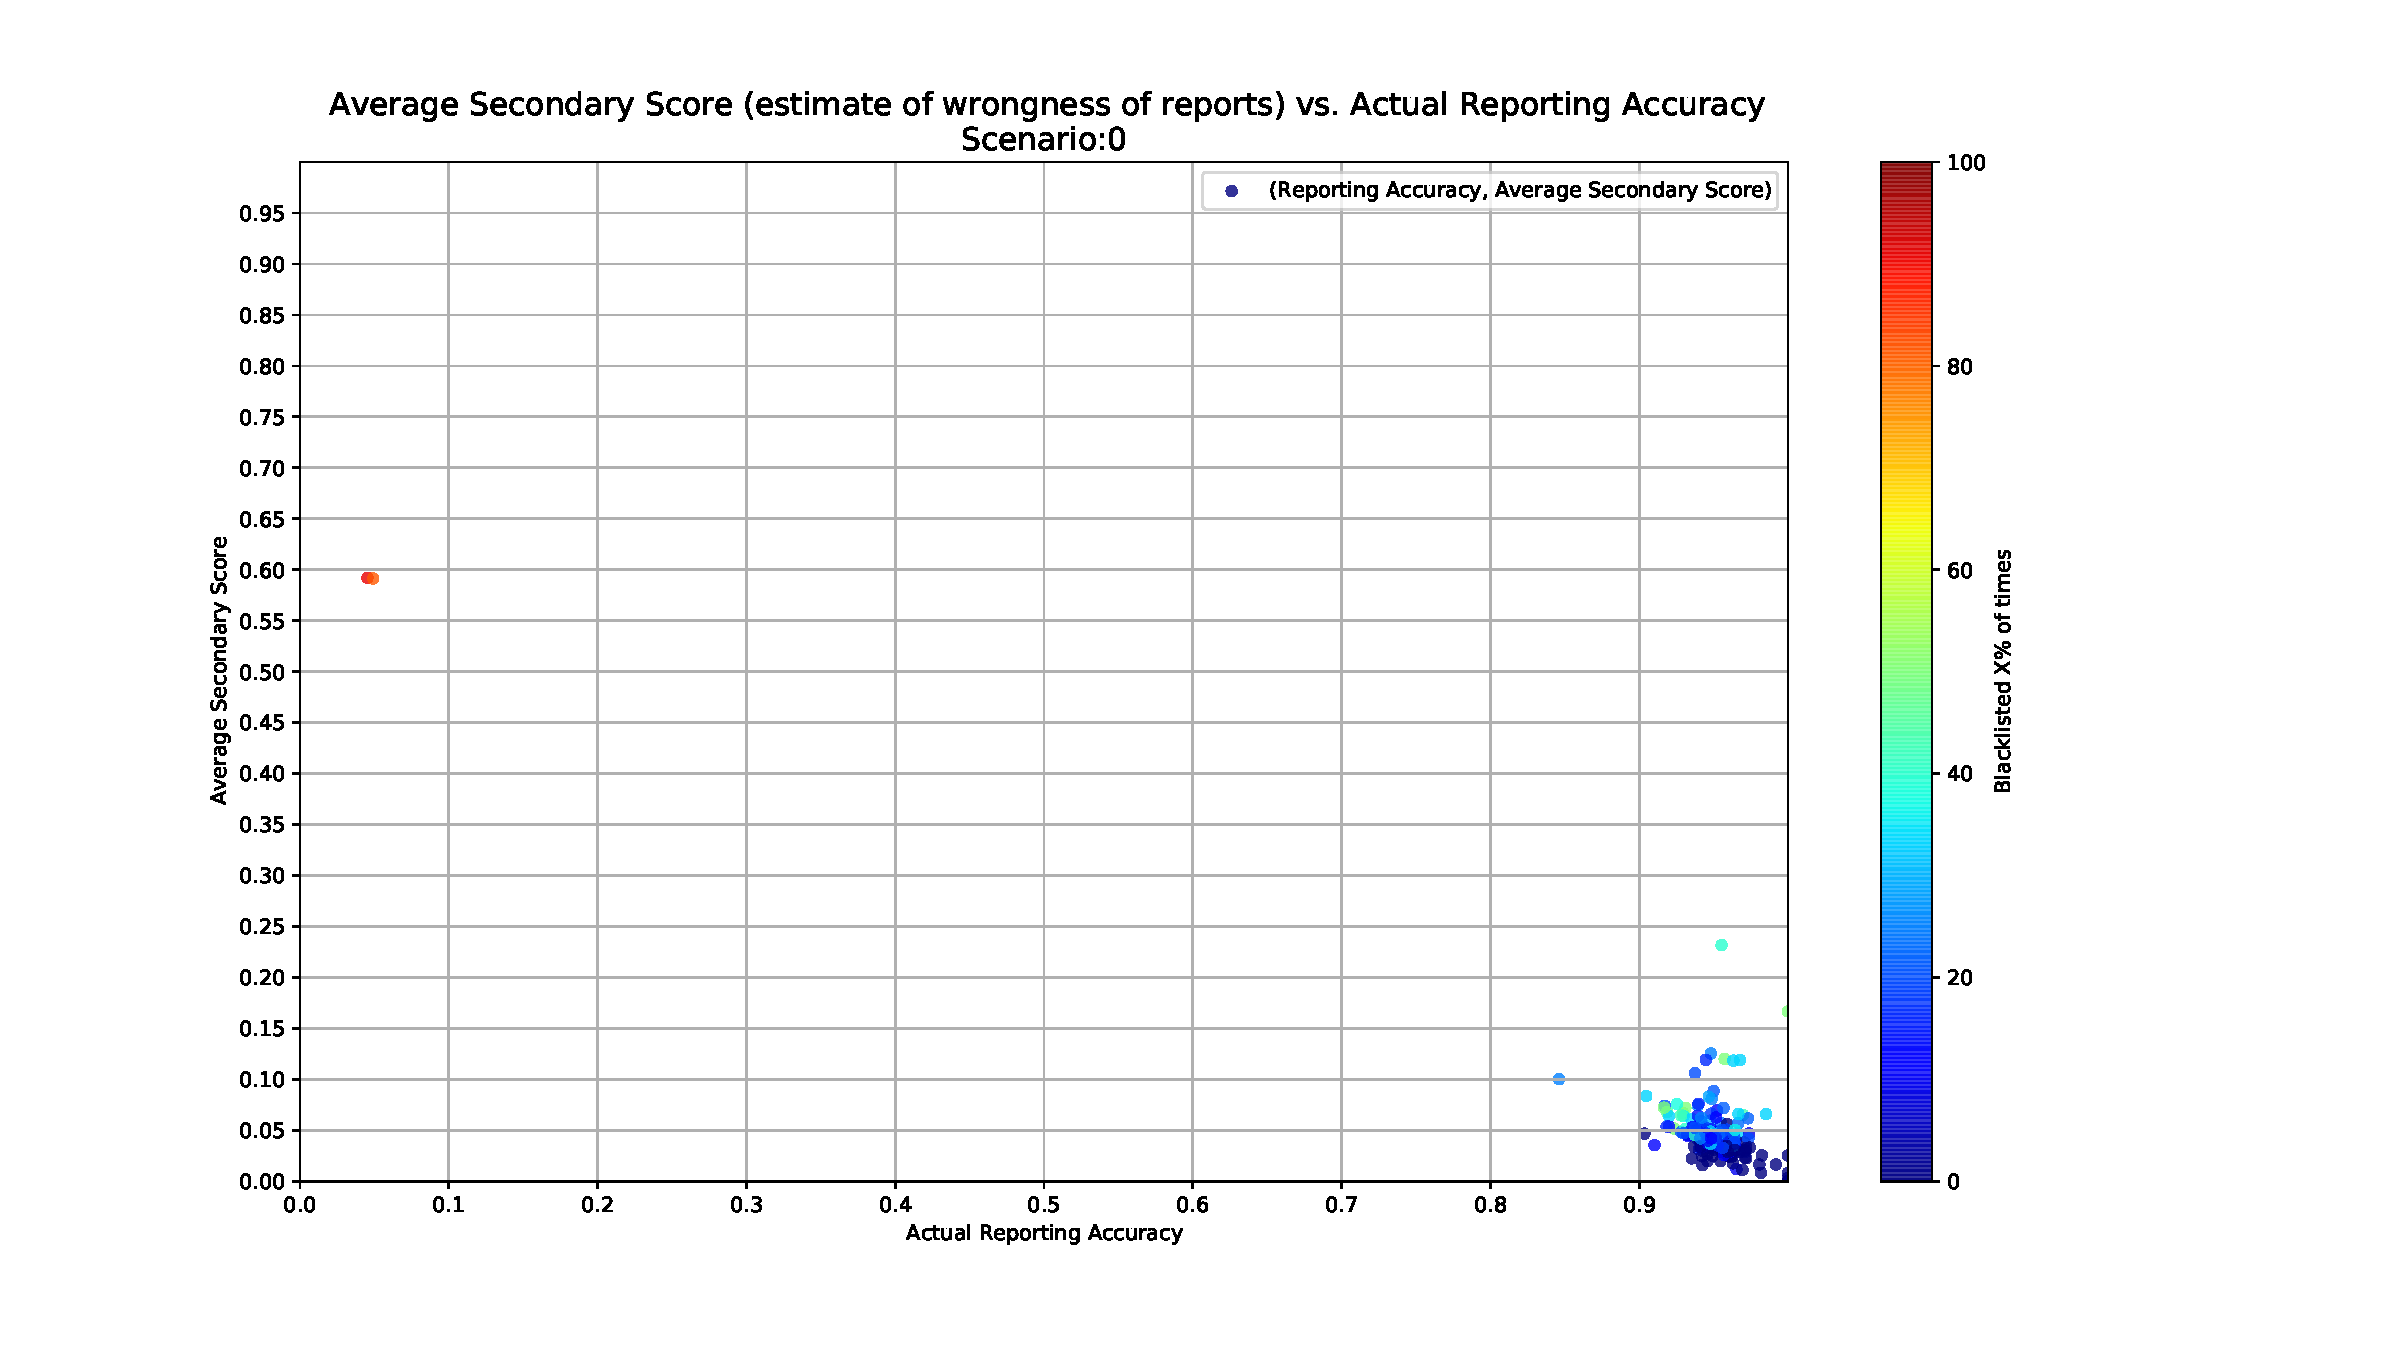
\includegraphics[width=0.5\linewidth,trim={100 50 185 72}, clip]{images/SCN0_ReportingAccuracy_Vs_AvgSecondaryScore.pdf}
		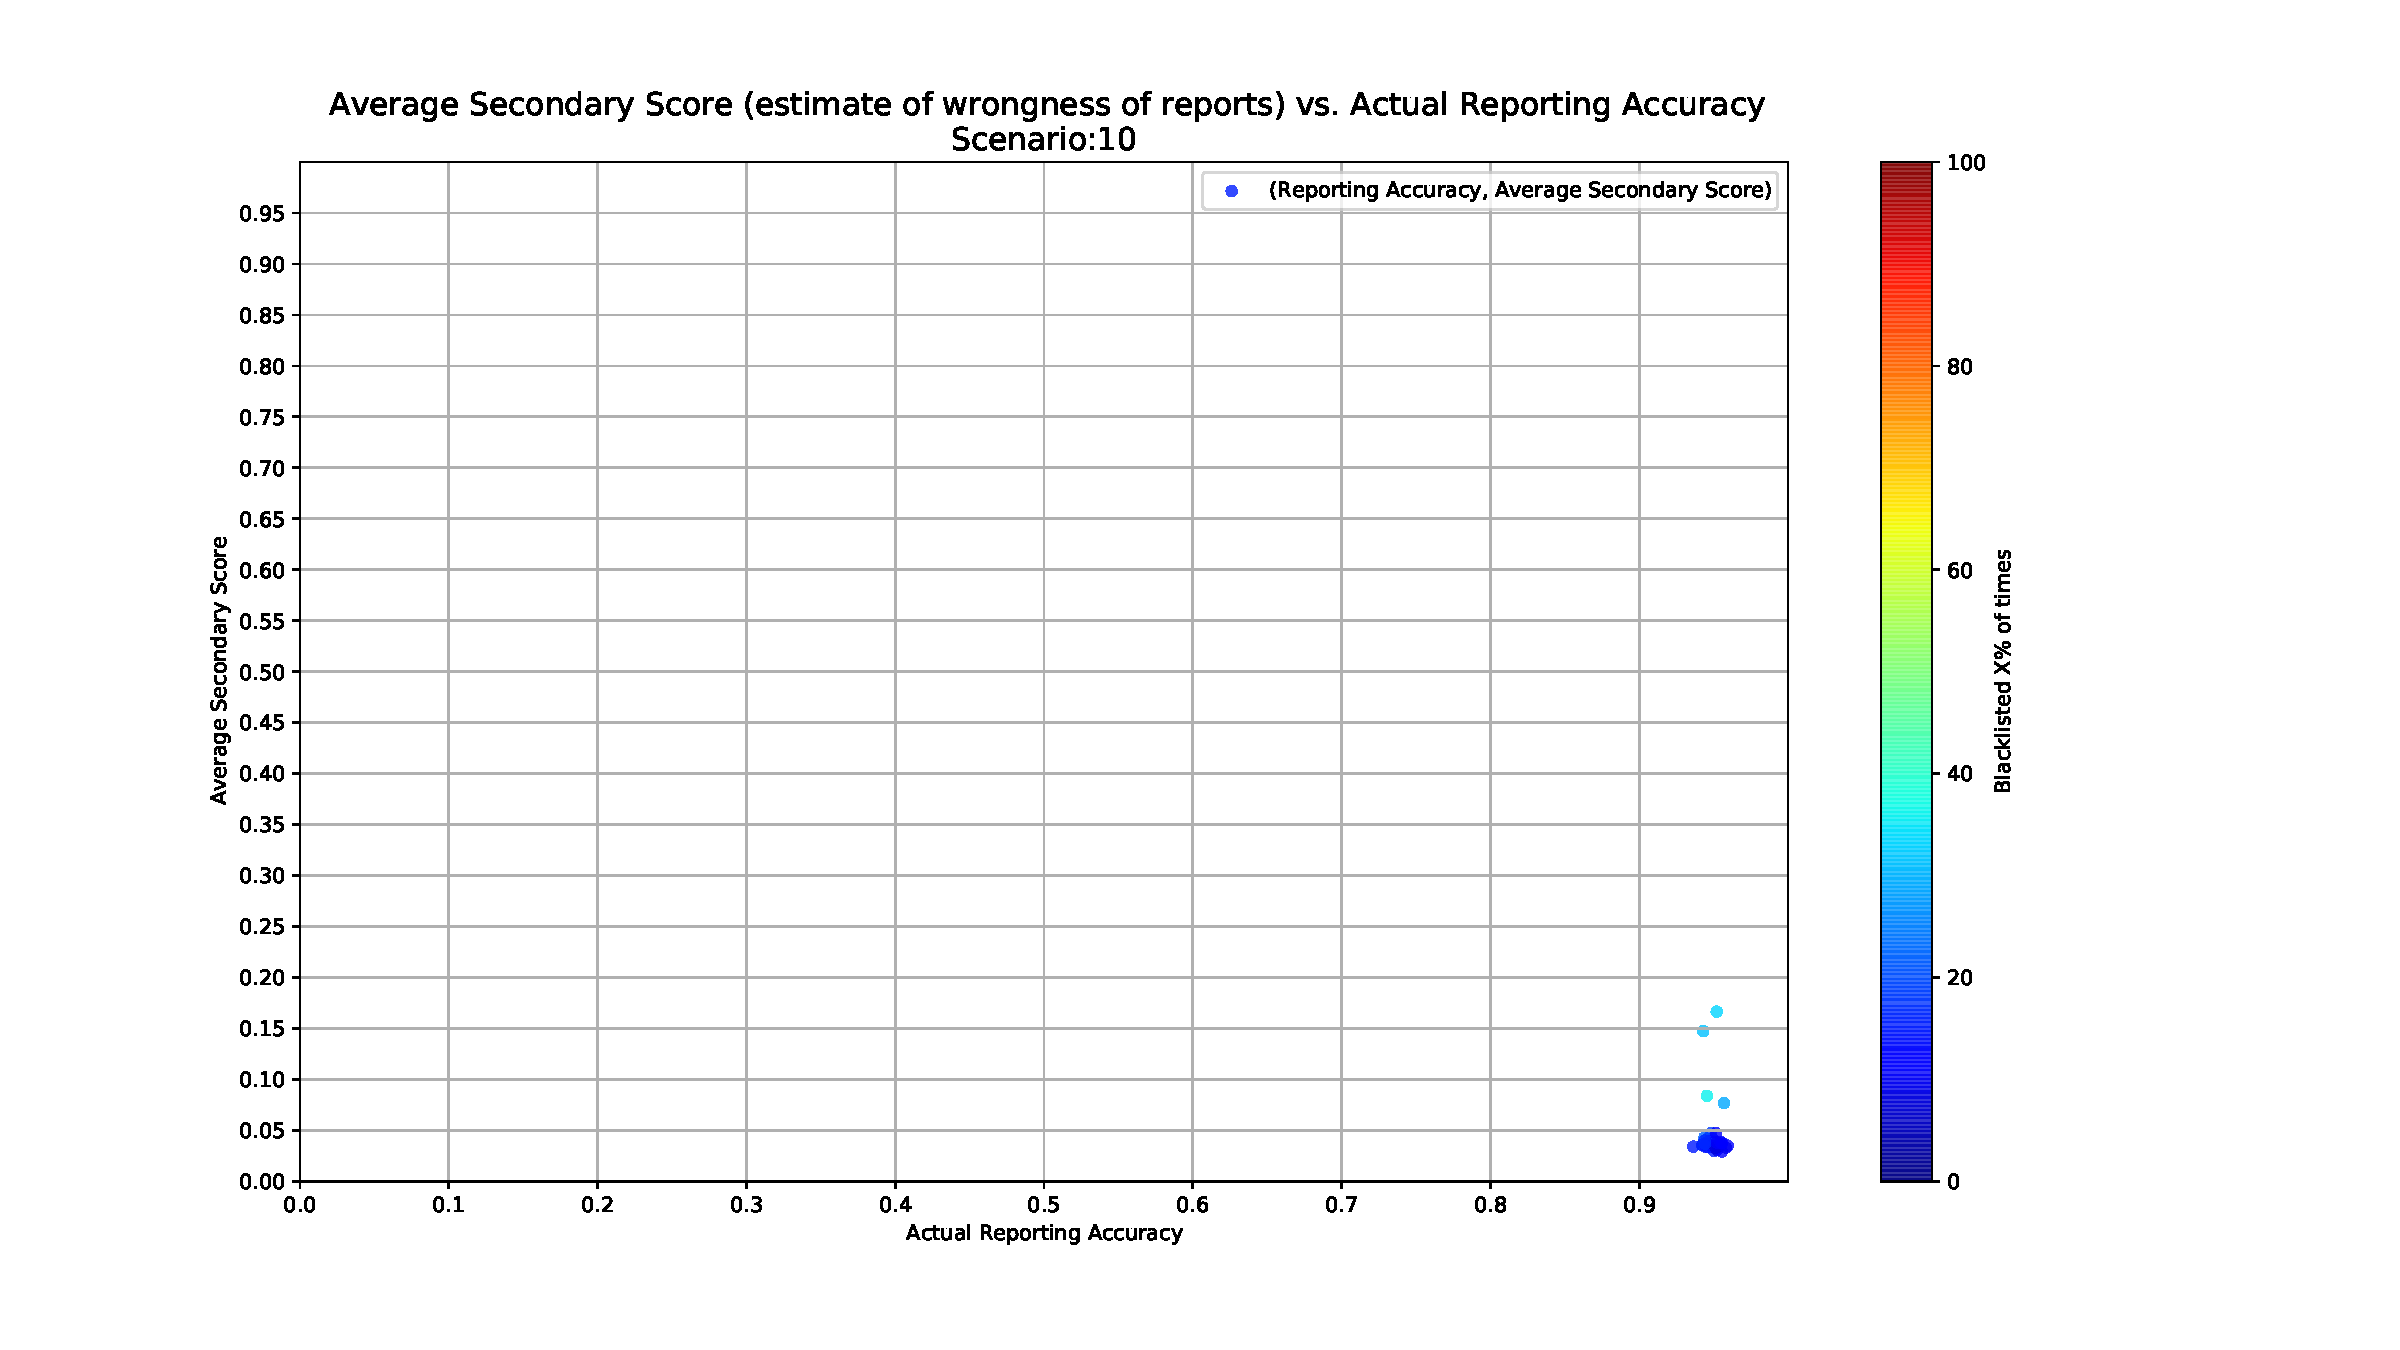
\includegraphics[width=0.5\linewidth,trim={100 50 185 72}, clip]{images/SCN10_ReportingAccuracy_Vs_AvgSecondaryScore.pdf}
	}
\end{figure*}
\begin{figure*}[!ht]
	\caption{Graphs for Results of Scenario 1 and 11. (a) Primary Score vs. Actual Accuracy - Scatter plot, without (above) and with (below) blacklisting for Scenario 1 (left) and Scenario 11 (right) (b) Absolute error (difference between actual accuracy of node and estimated accuracy) vs. Percentage of nodes for which there was less than 'x'\% error for Scenario 1 (left) and Scenario 11 (right) (c) Mean Secondary Score vs. Accuracy of Reports Sent - Scatter plot for Scenario 1 (left) and Scenario 11 (right)}
	\label{fig:apdx:ev1}
	\centering
	\subfloat[]{
		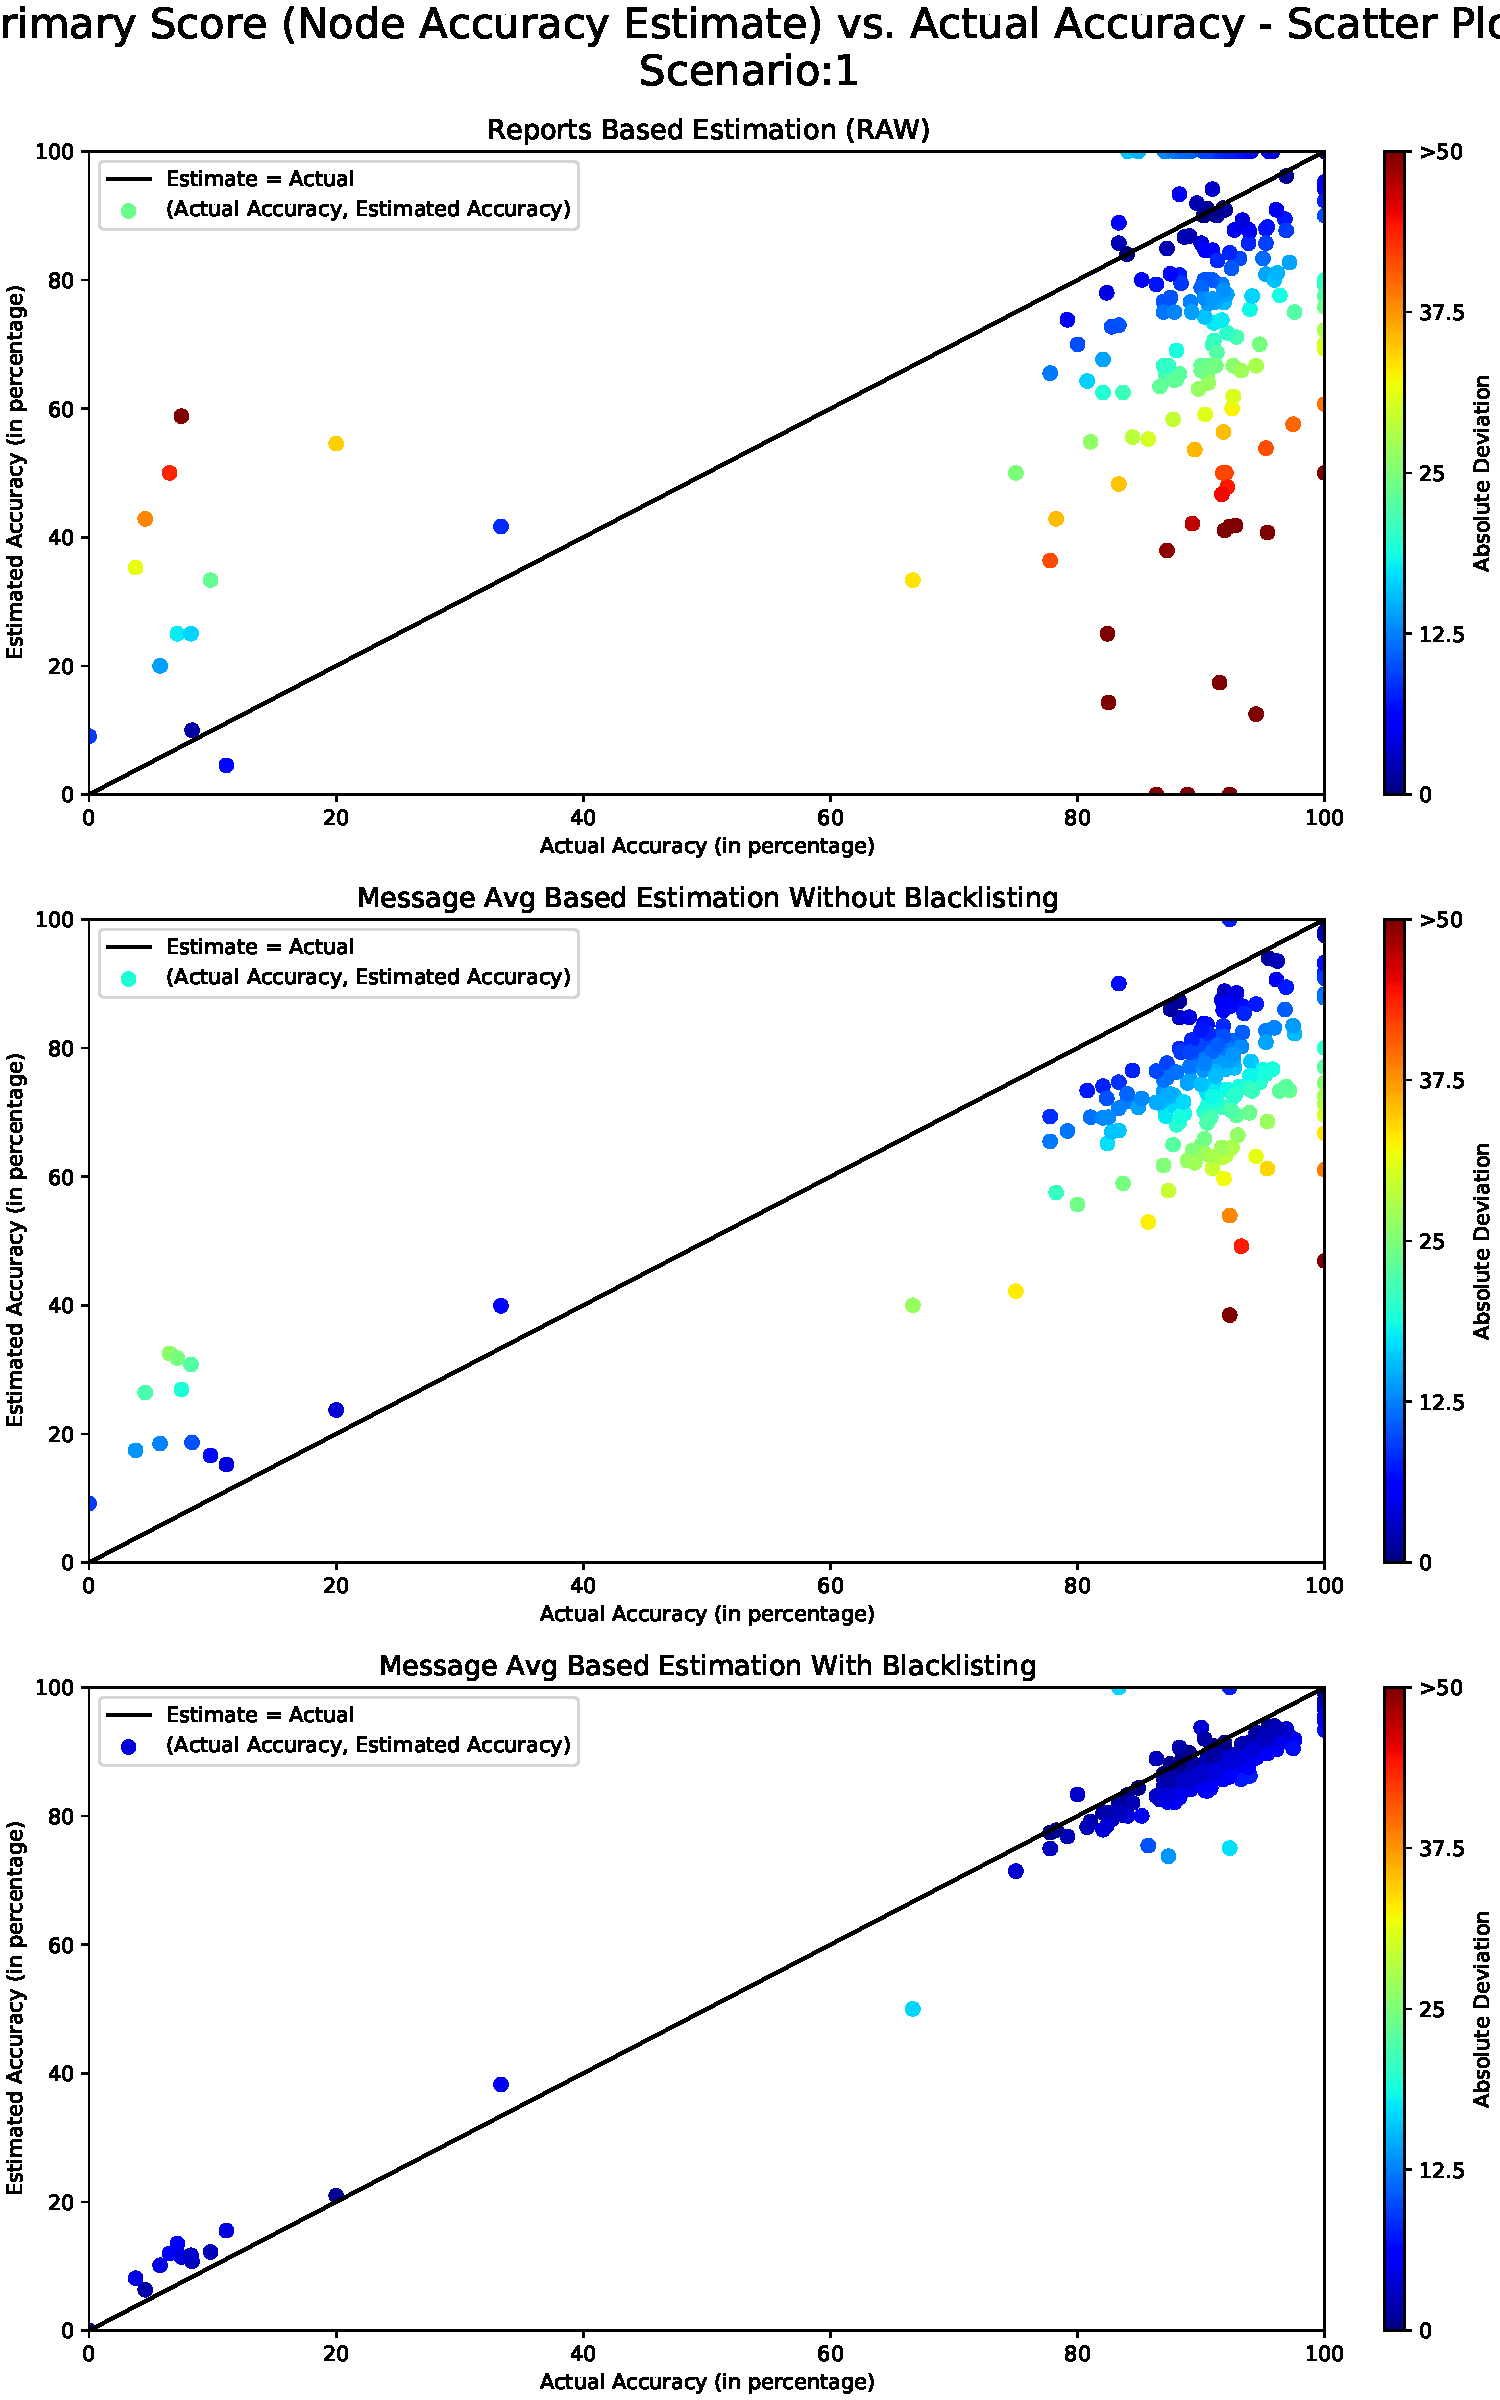
\includegraphics[width=0.5\linewidth, trim={0 5 15 420}, clip]{images/SCN1_PrimaryScoreVsActualAccuracyComparitive.pdf}
		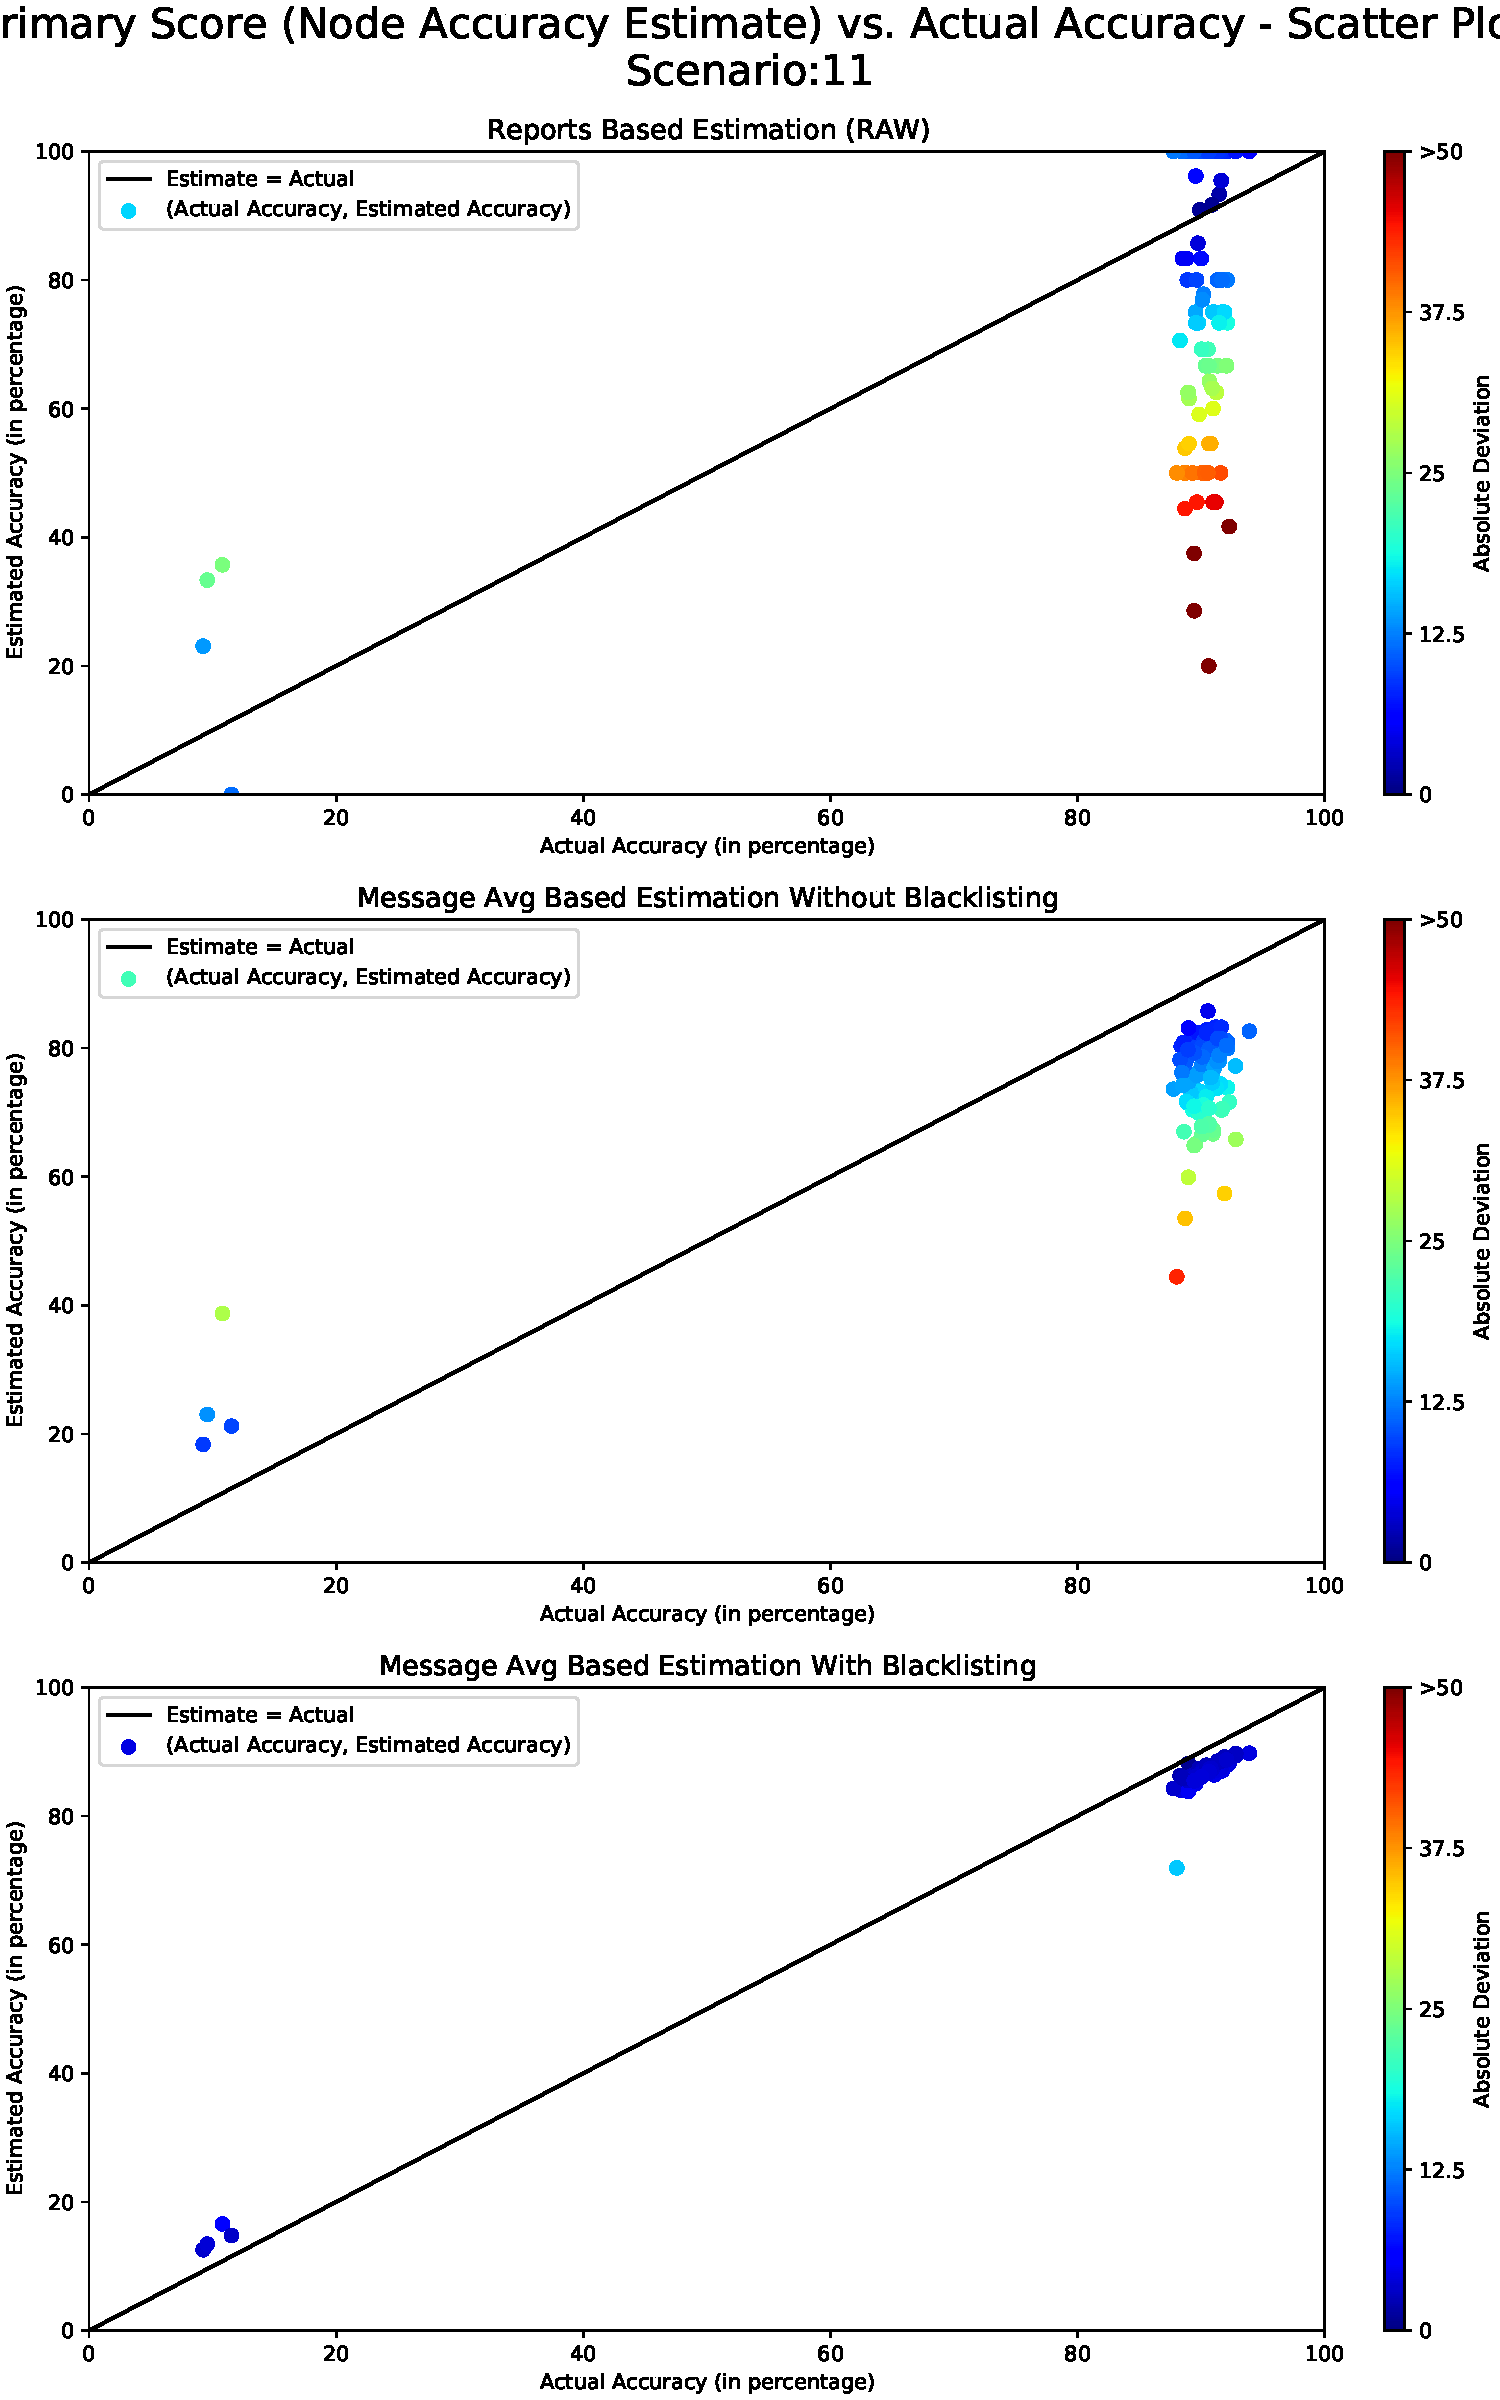
\includegraphics[width=0.5\linewidth, trim={0 5 15 420}, clip]{images/SCN11_PrimaryScoreVsActualAccuracyComparitive.pdf}
	} \\\vfill
	\subfloat[]{
		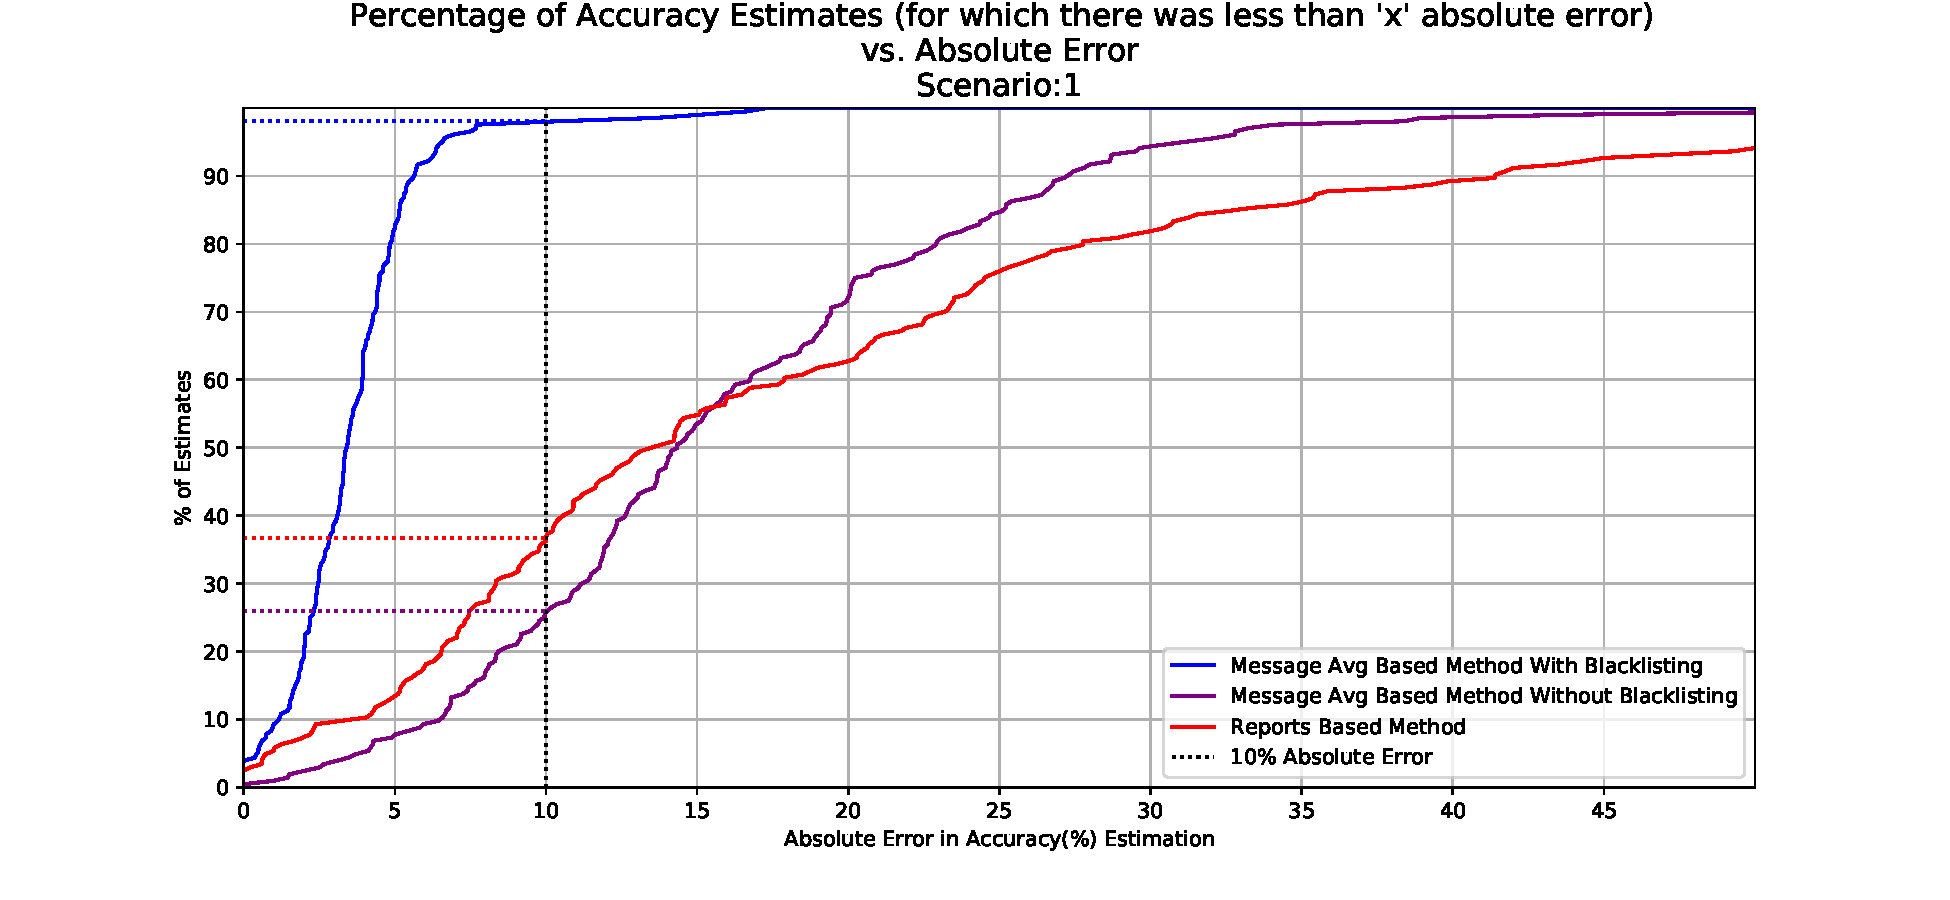
\includegraphics[width=0.5\linewidth, trim={80 25 90 50}, clip]{images/SCN1_AbsoluteErrorsInEstimationComparison.pdf}
		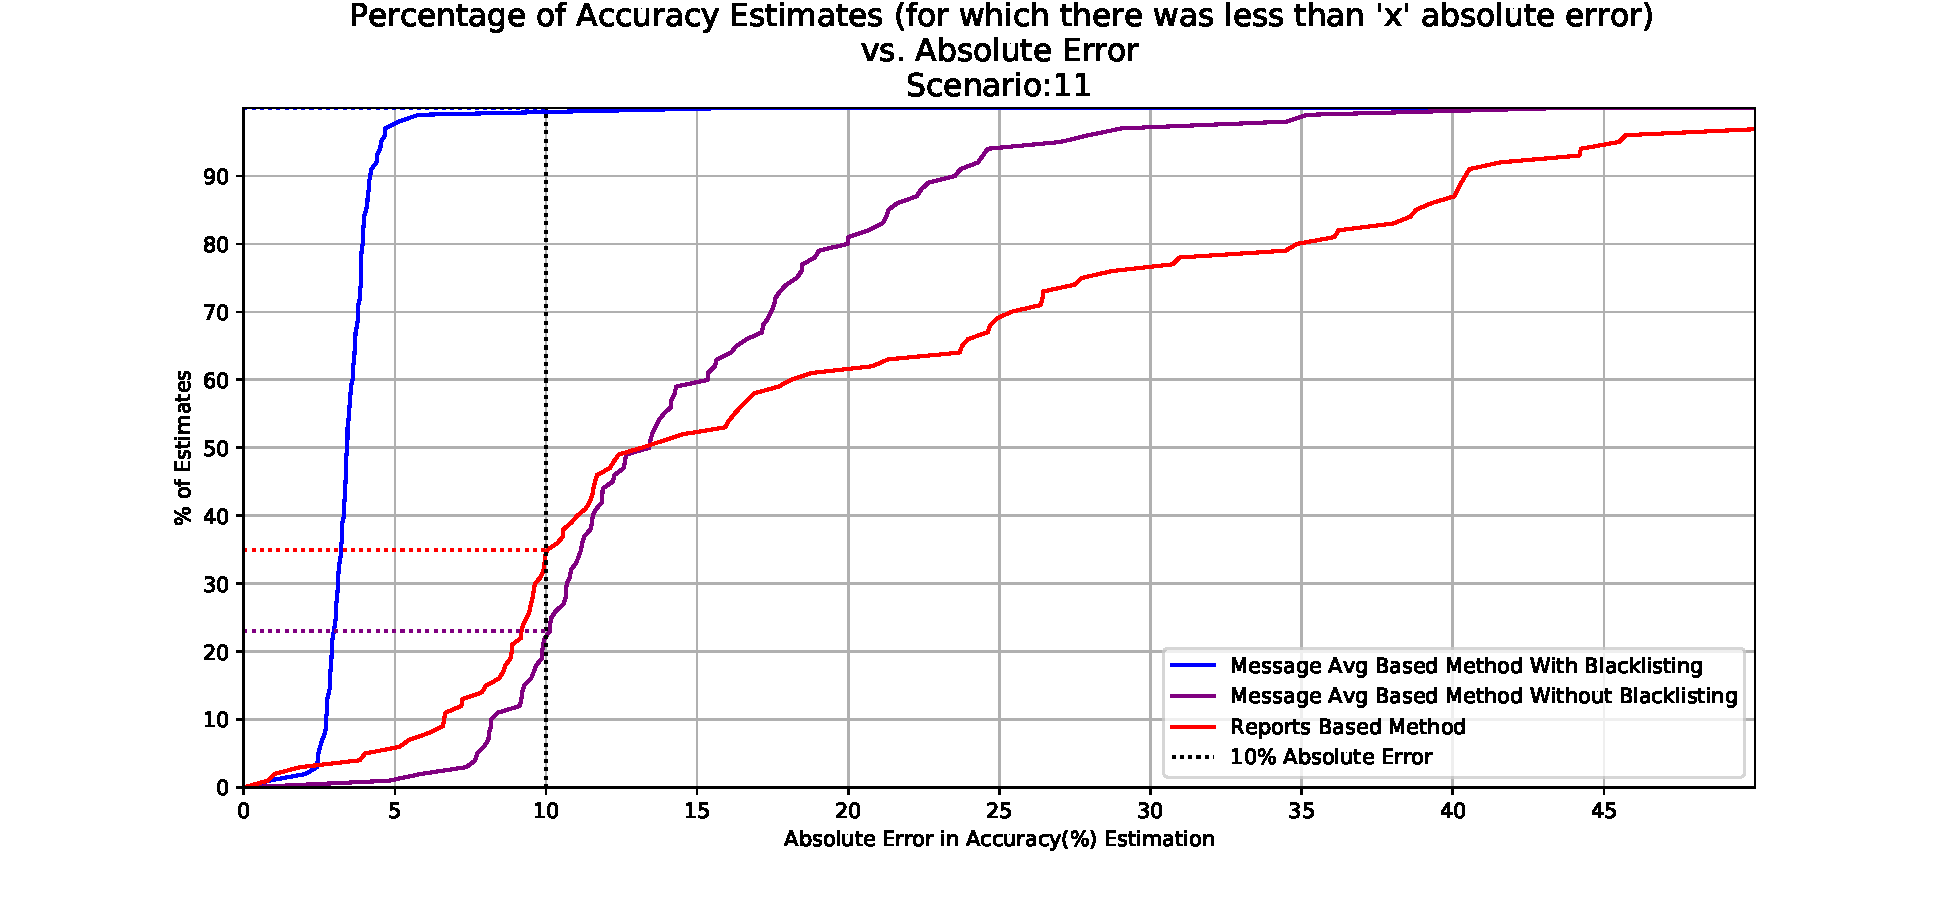
\includegraphics[width=0.5\linewidth, trim={80 25 90 50}, clip]{images/SCN11_AbsoluteErrorsInEstimationComparison.pdf}
	}
	\hfill
	\subfloat[]{
		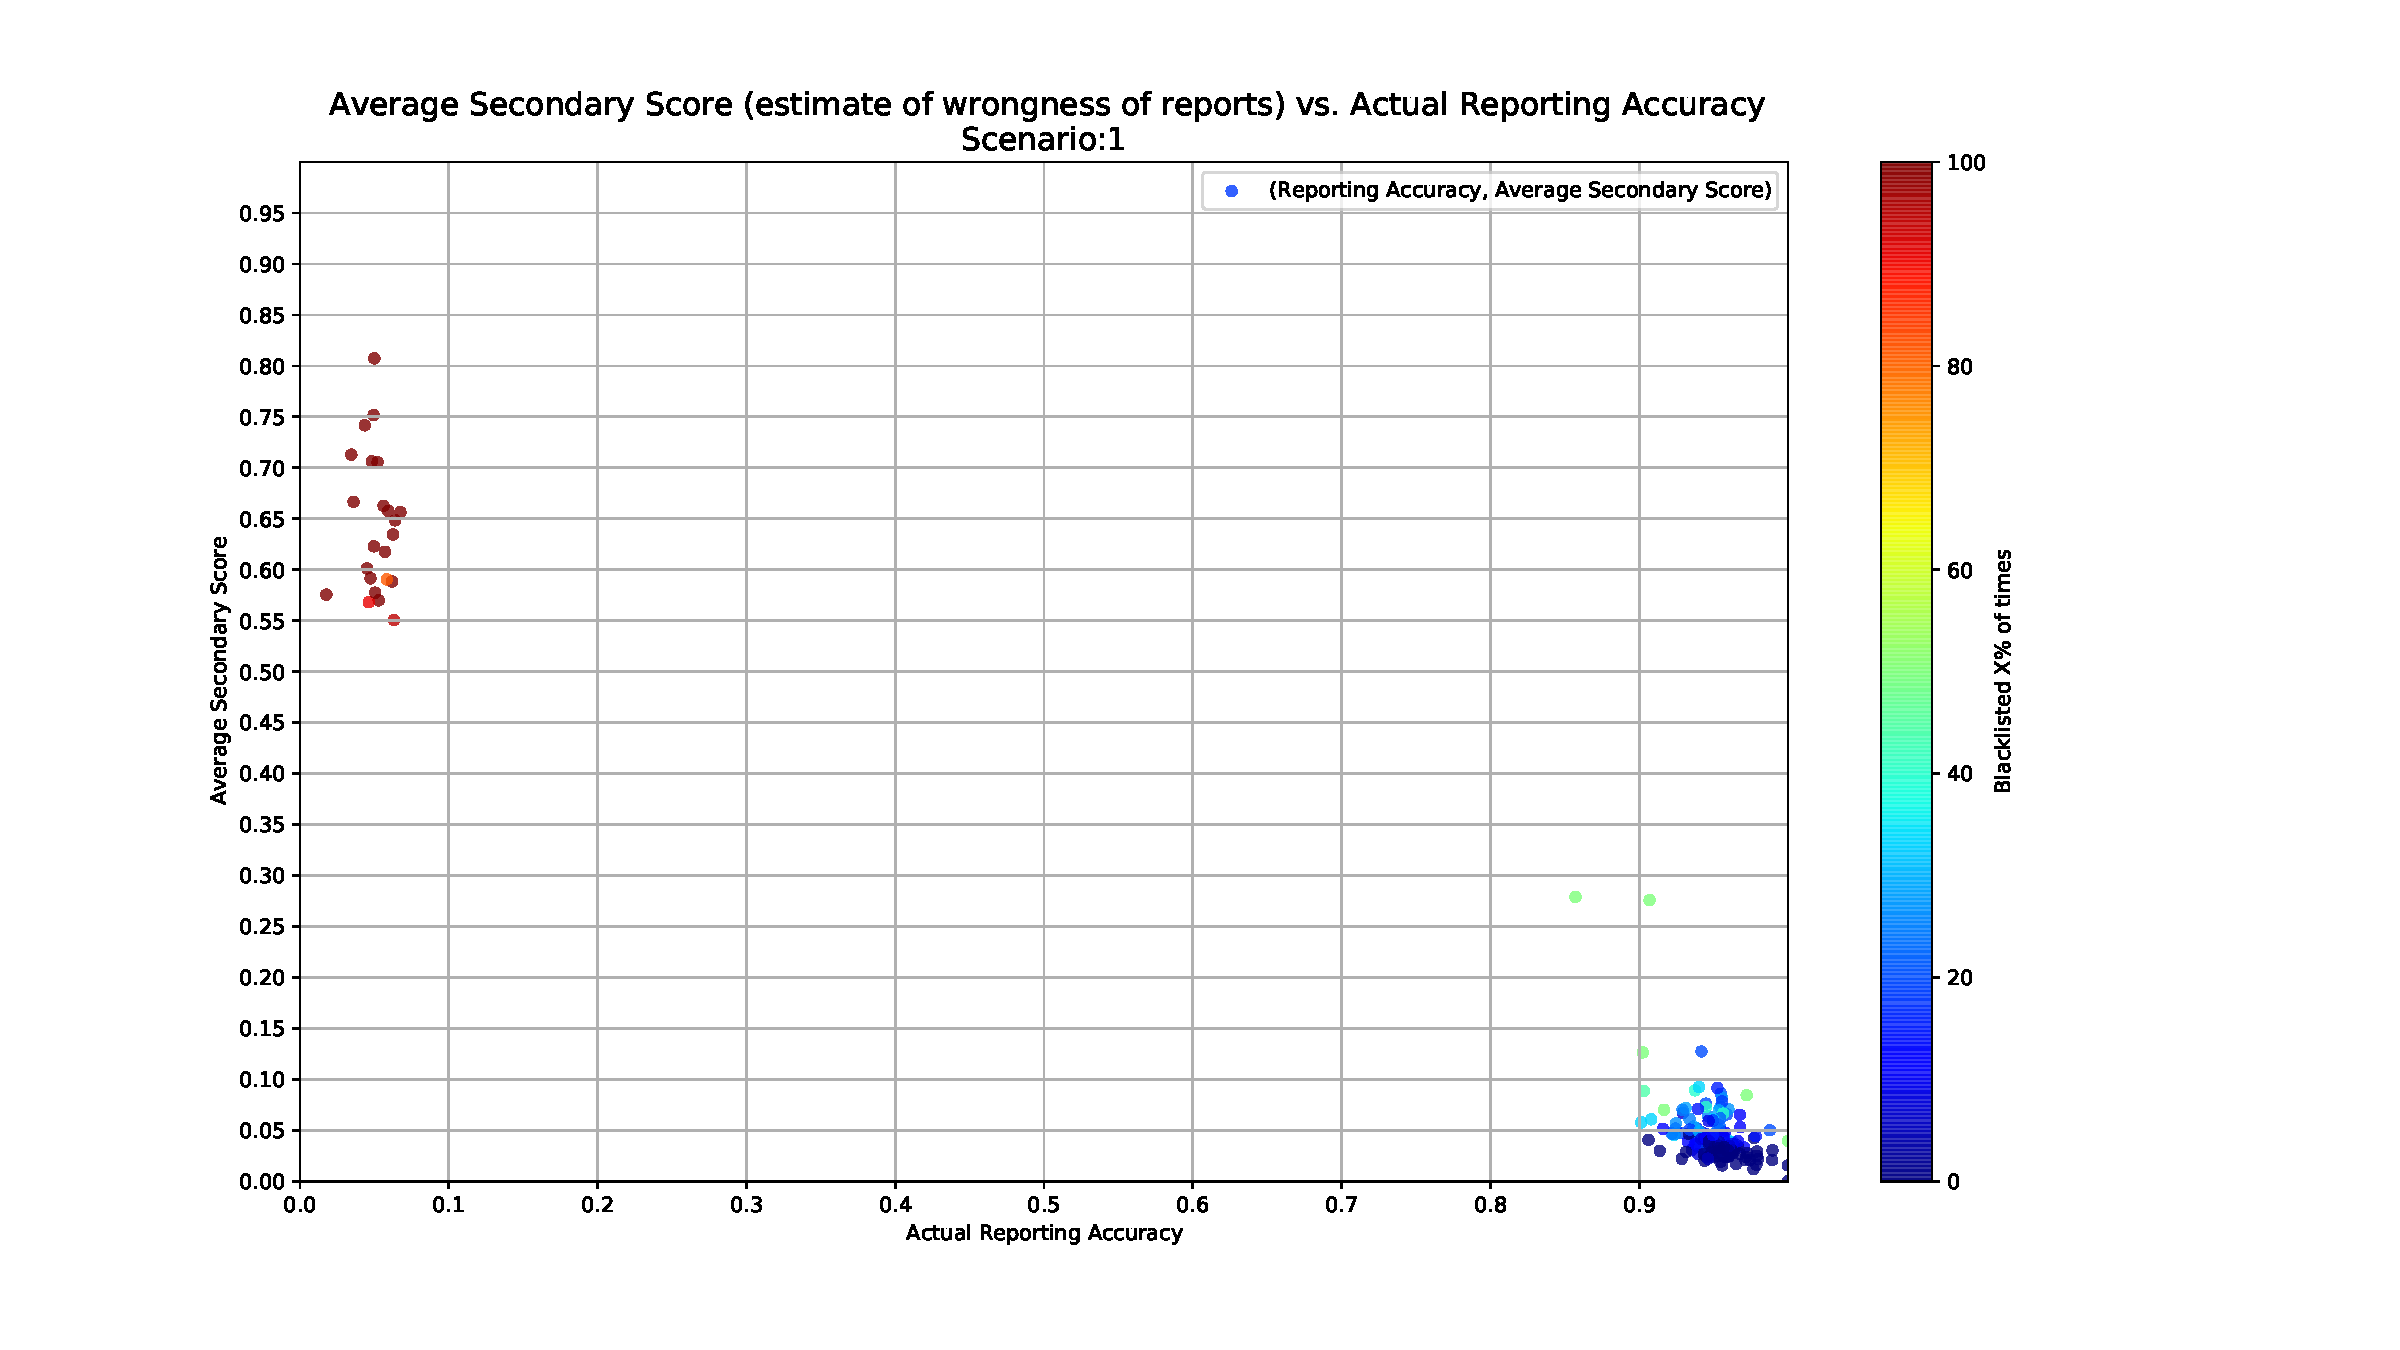
\includegraphics[width=0.5\linewidth,trim={100 50 185 72}, clip]{images/SCN1_ReportingAccuracy_Vs_AvgSecondaryScore.pdf}
		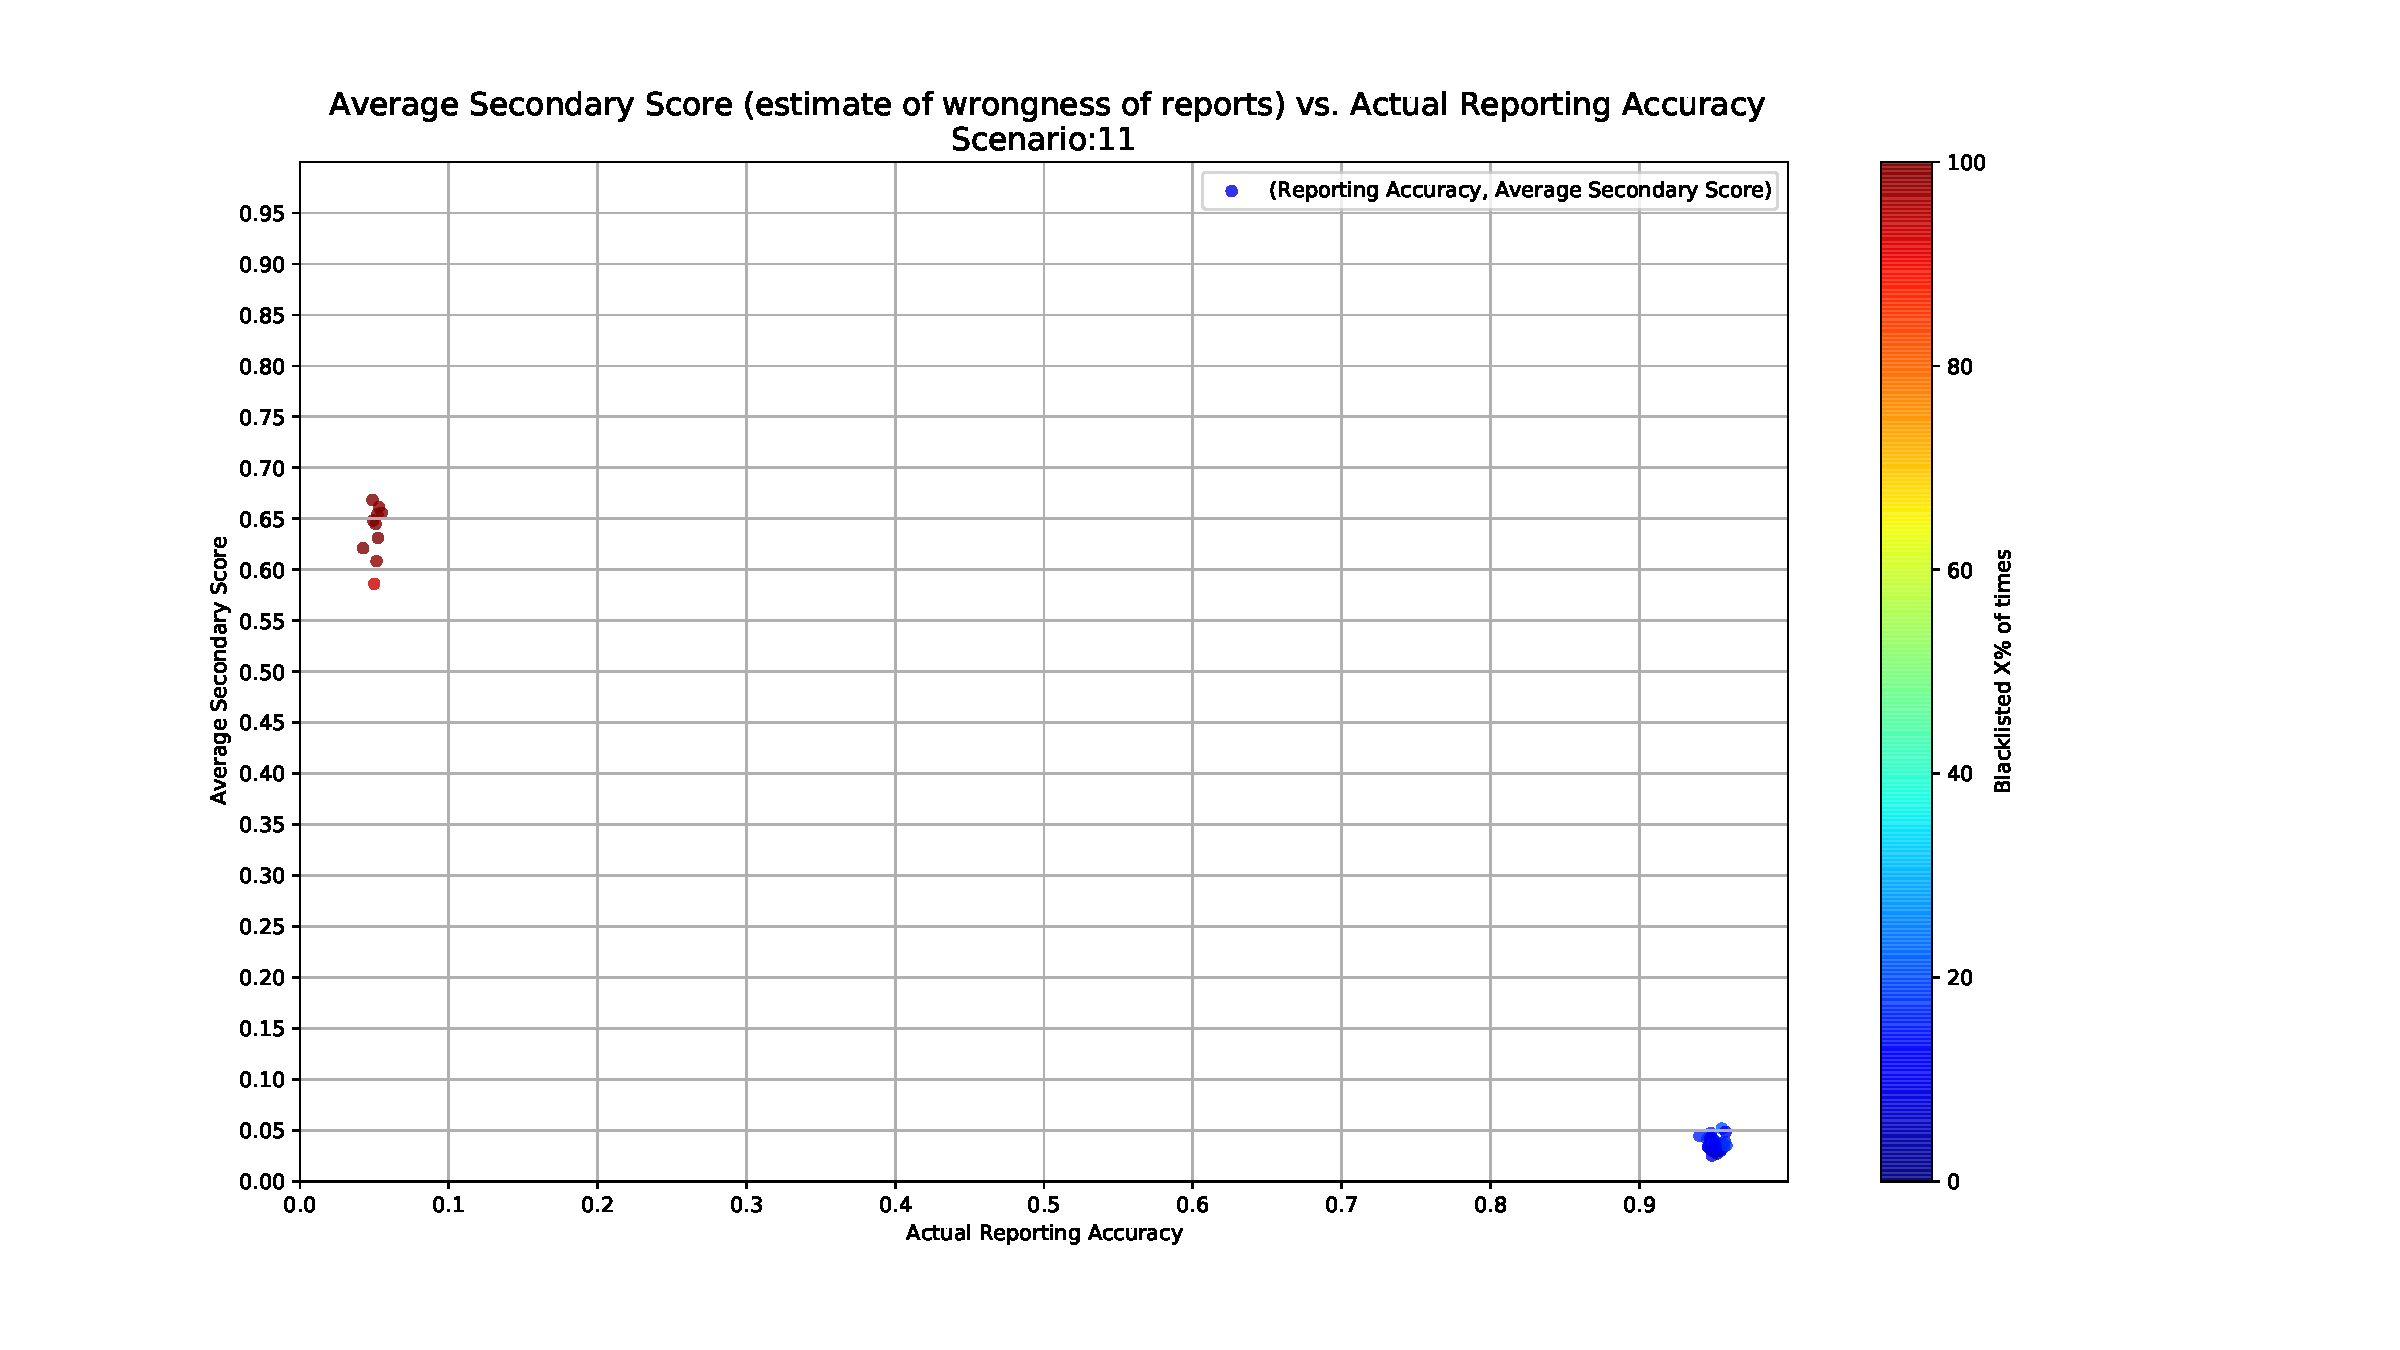
\includegraphics[width=0.5\linewidth,trim={100 50 185 72}, clip]{images/SCN11_ReportingAccuracy_Vs_AvgSecondaryScore.pdf}
	}
\end{figure*}
\begin{figure*}[!ht]
	\caption{Graphs for Results of Scenario 2 and 12. (a) Primary Score vs. Actual Accuracy - Scatter plot, without (above) and with (below) blacklisting for Scenario 2 (left) and Scenario 12 (right) (b) Absolute error (difference between actual accuracy of node and estimated accuracy) vs. Percentage of nodes for which there was less than 'x'\% error for Scenario 2 (left) and Scenario 12 (right) (c) Mean Secondary Score vs. Accuracy of Reports Sent - Scatter plot for Scenario 2 (left) and Scenario 12 (right)}
	\label{fig:apdx:ev2}
	\centering
	\subfloat[]{
		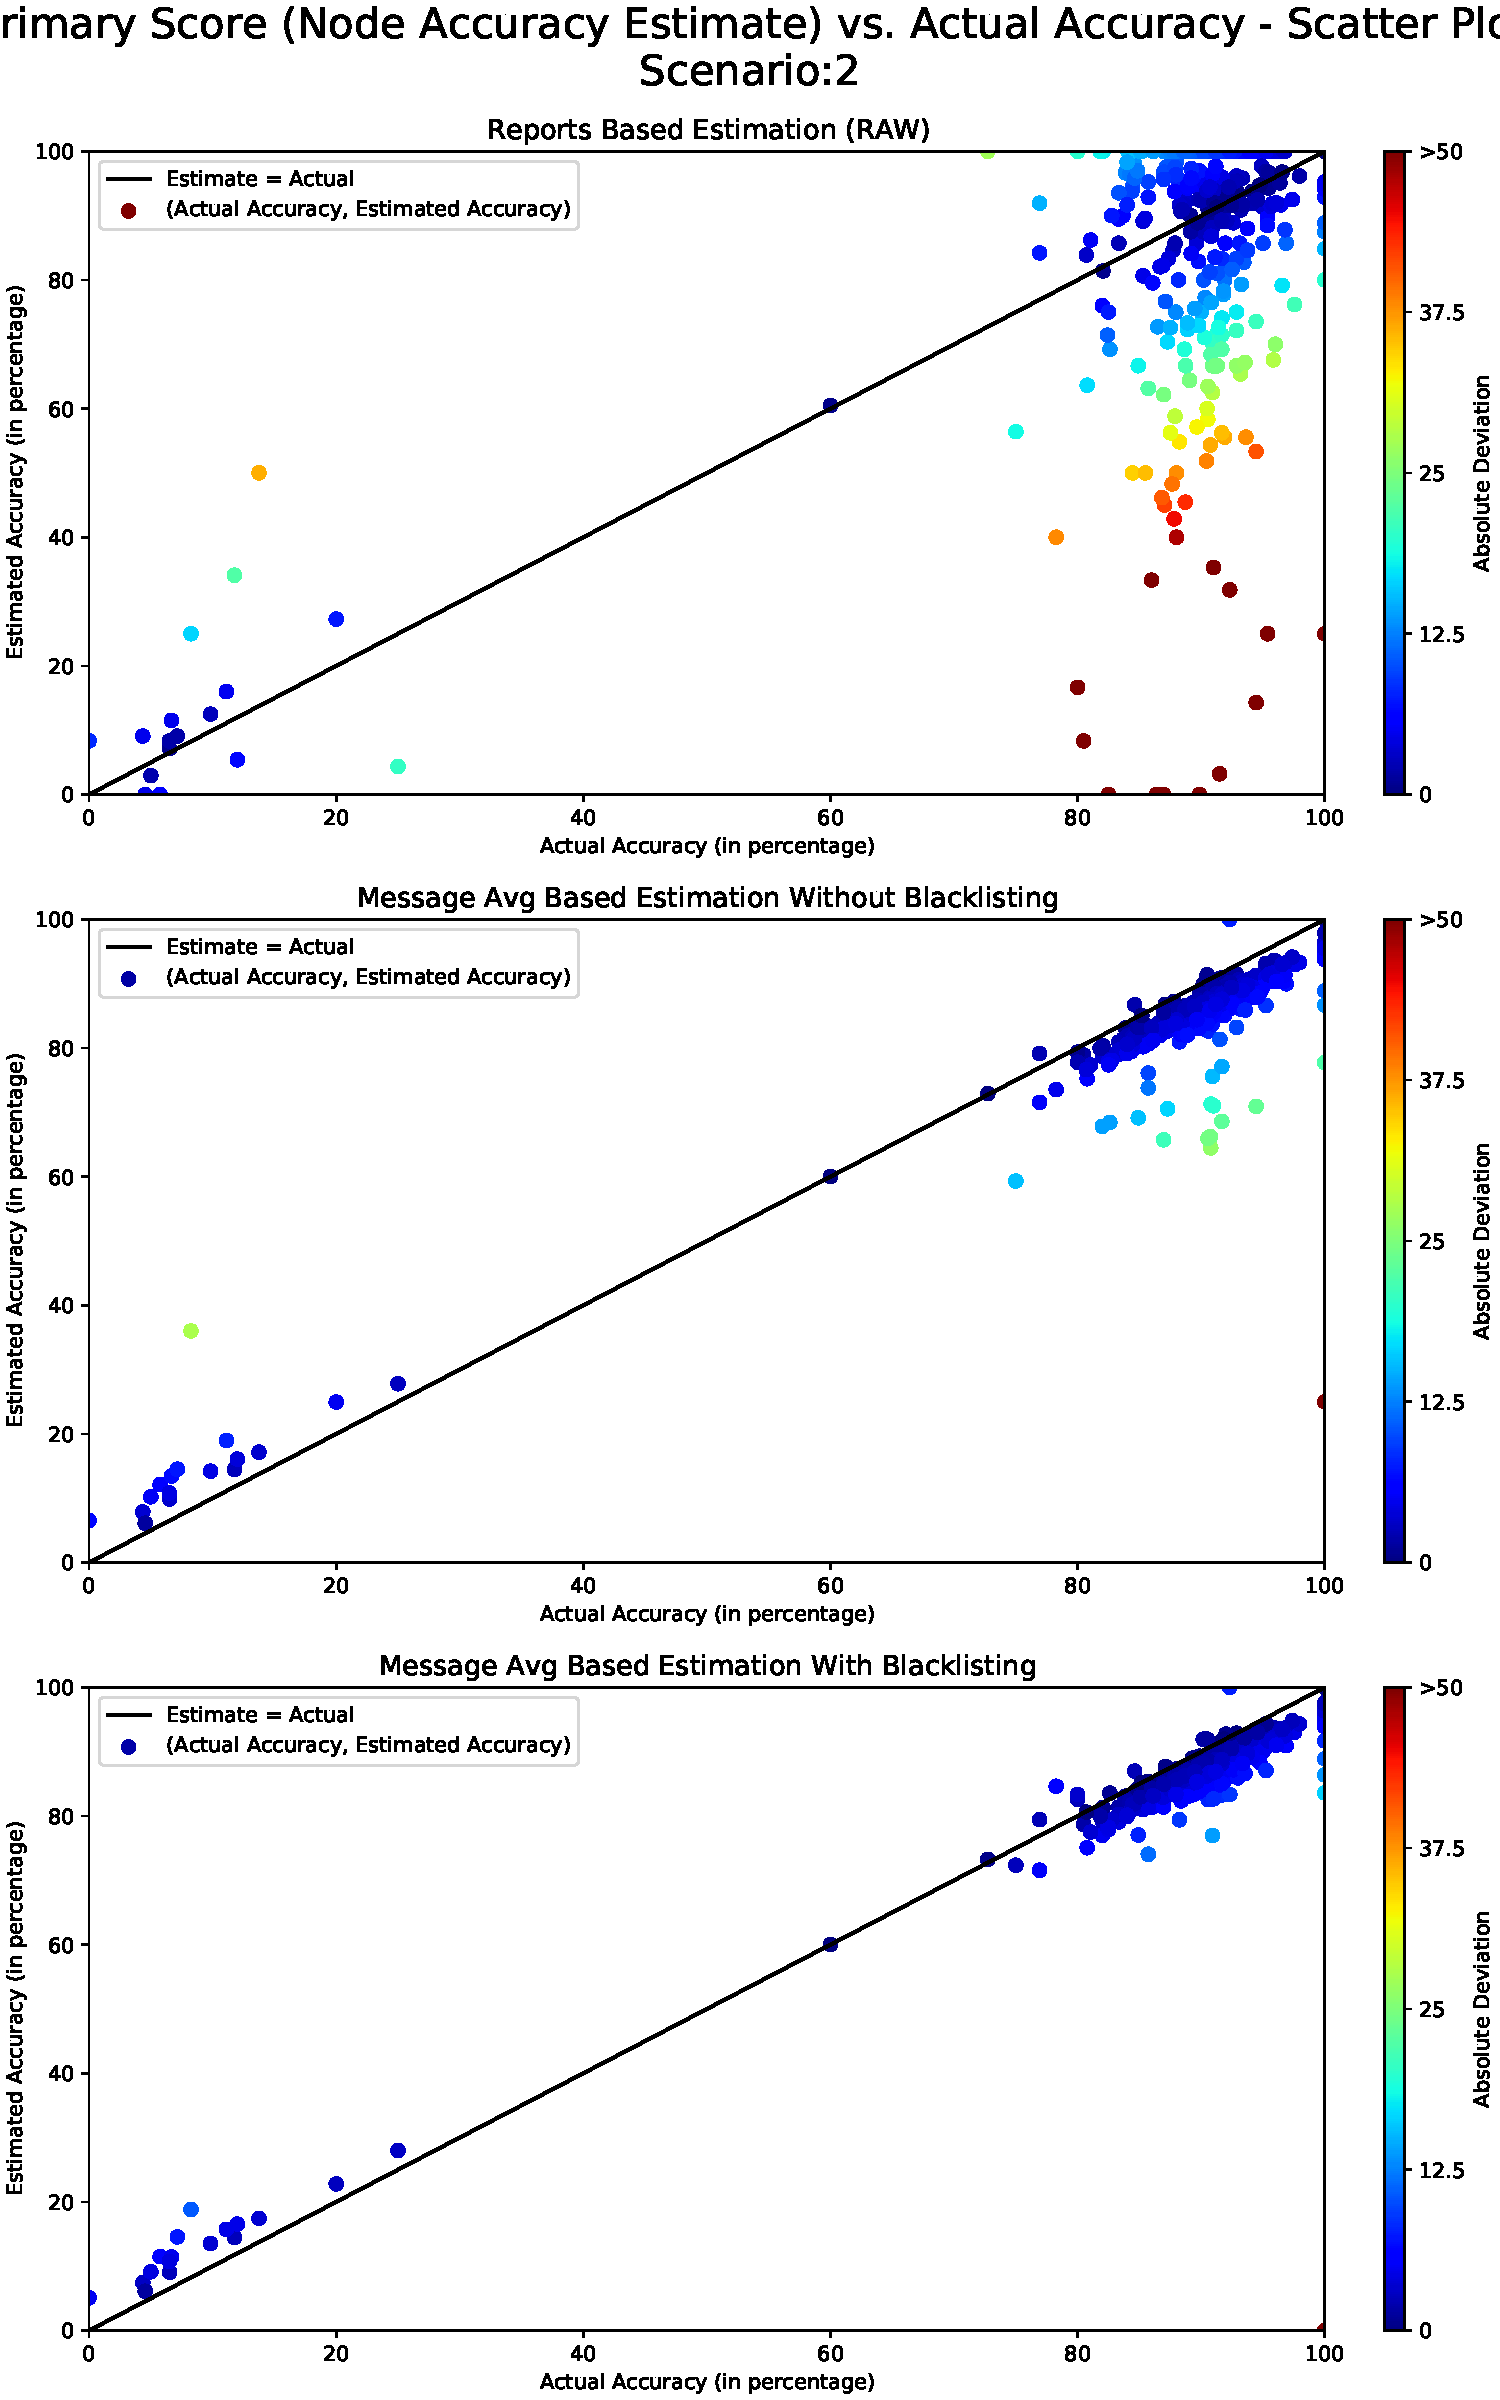
\includegraphics[width=0.5\linewidth, trim={0 5 15 420}, clip]{images/SCN2_PrimaryScoreVsActualAccuracyComparitive.pdf}
		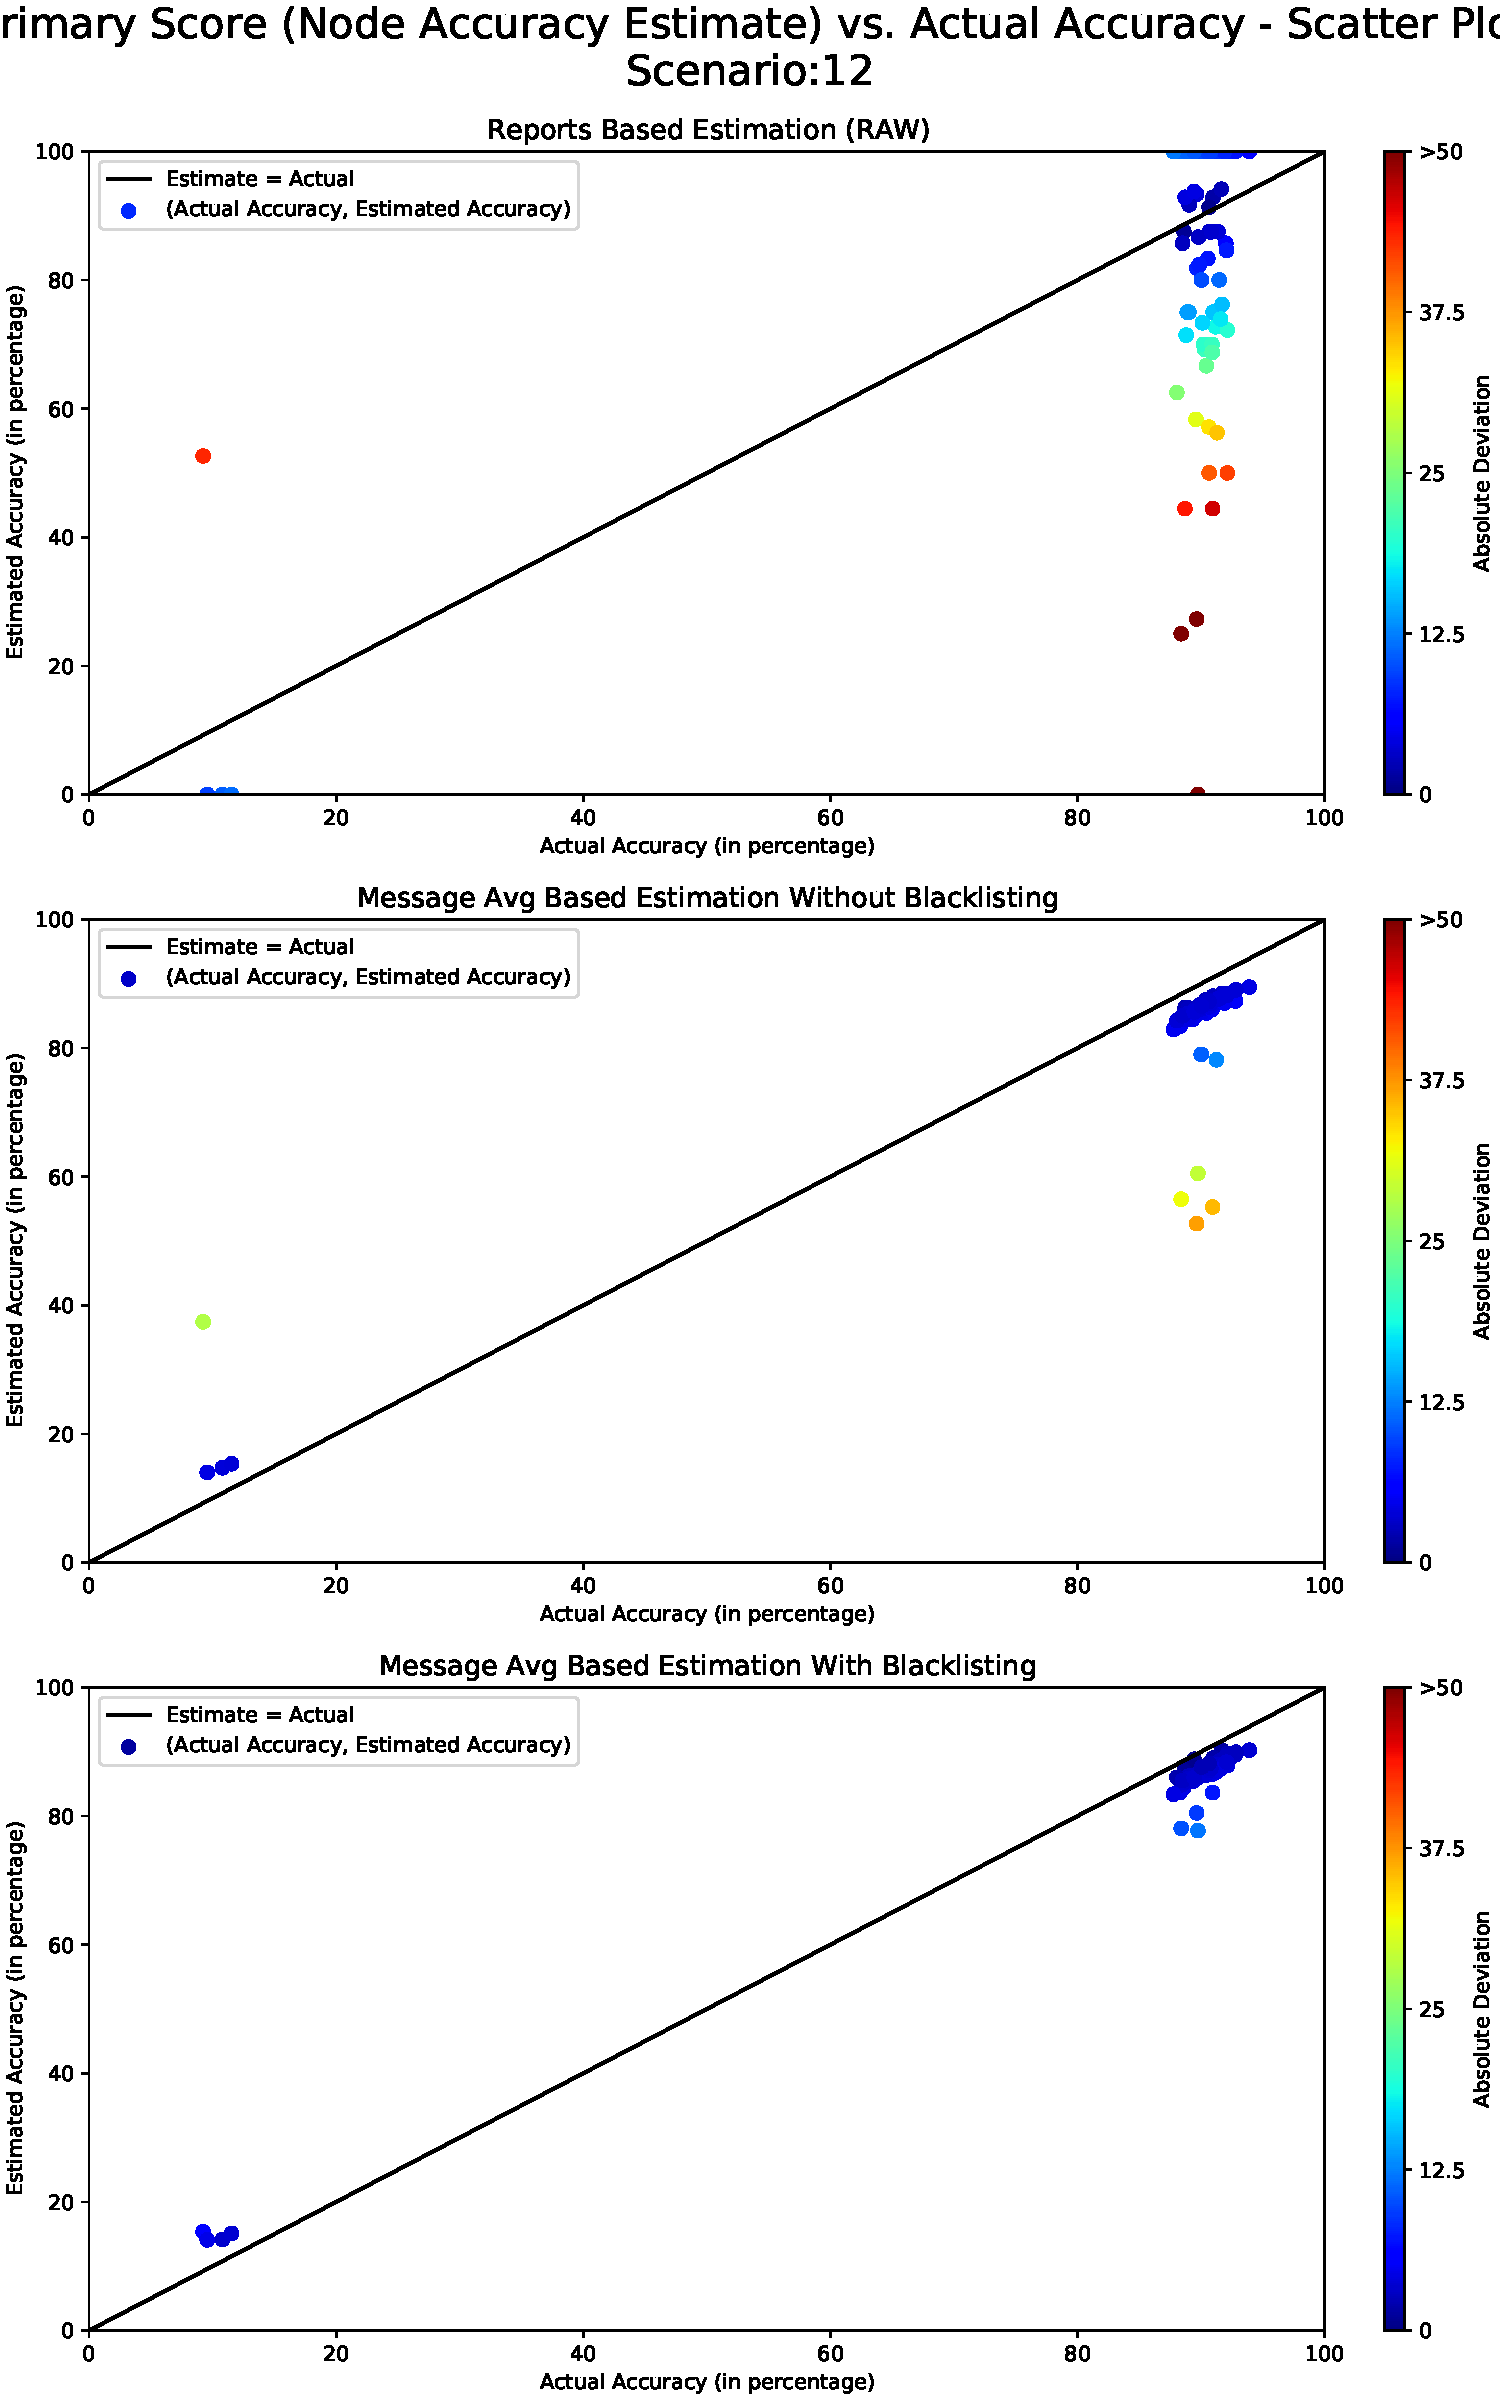
\includegraphics[width=0.5\linewidth, trim={0 5 15 420}, clip]{images/SCN12_PrimaryScoreVsActualAccuracyComparitive.pdf}
	} \\\vfill
	\subfloat[]{
		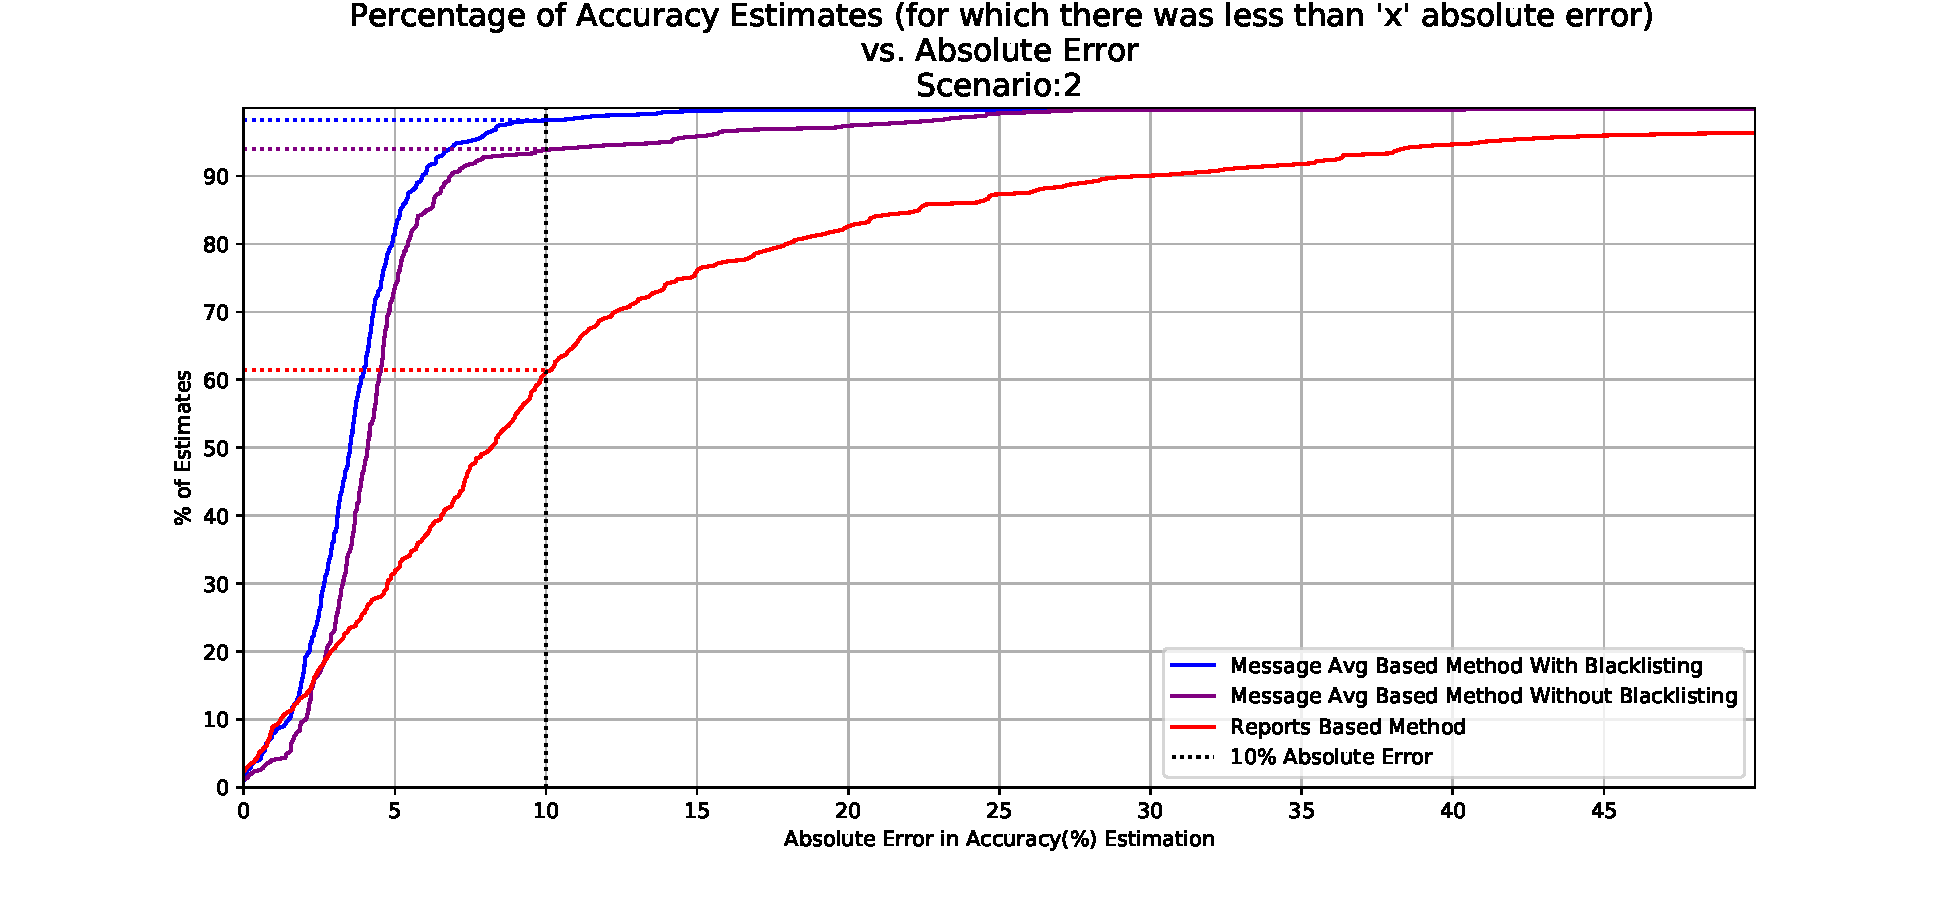
\includegraphics[width=0.5\linewidth, trim={80 25 90 50}, clip]{images/SCN2_AbsoluteErrorsInEstimationComparison.pdf}
		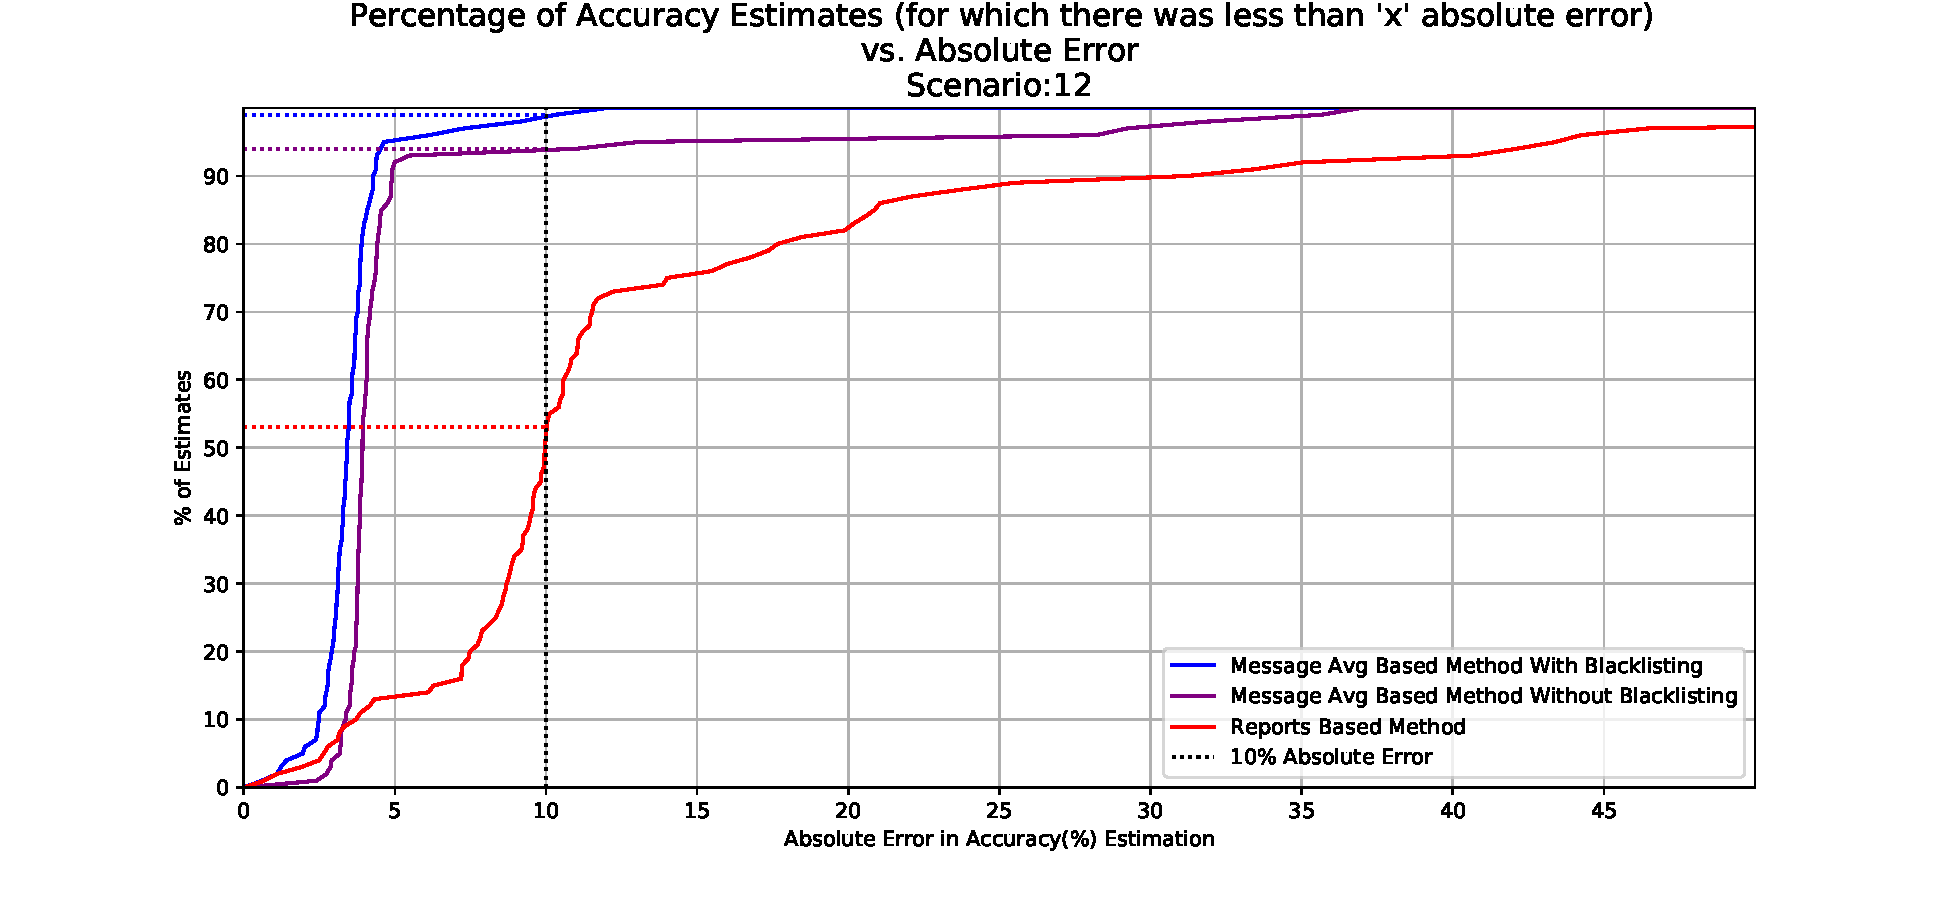
\includegraphics[width=0.5\linewidth, trim={80 25 90 50}, clip]{images/SCN12_AbsoluteErrorsInEstimationComparison.pdf}
	}
	\hfill
	\subfloat[]{
		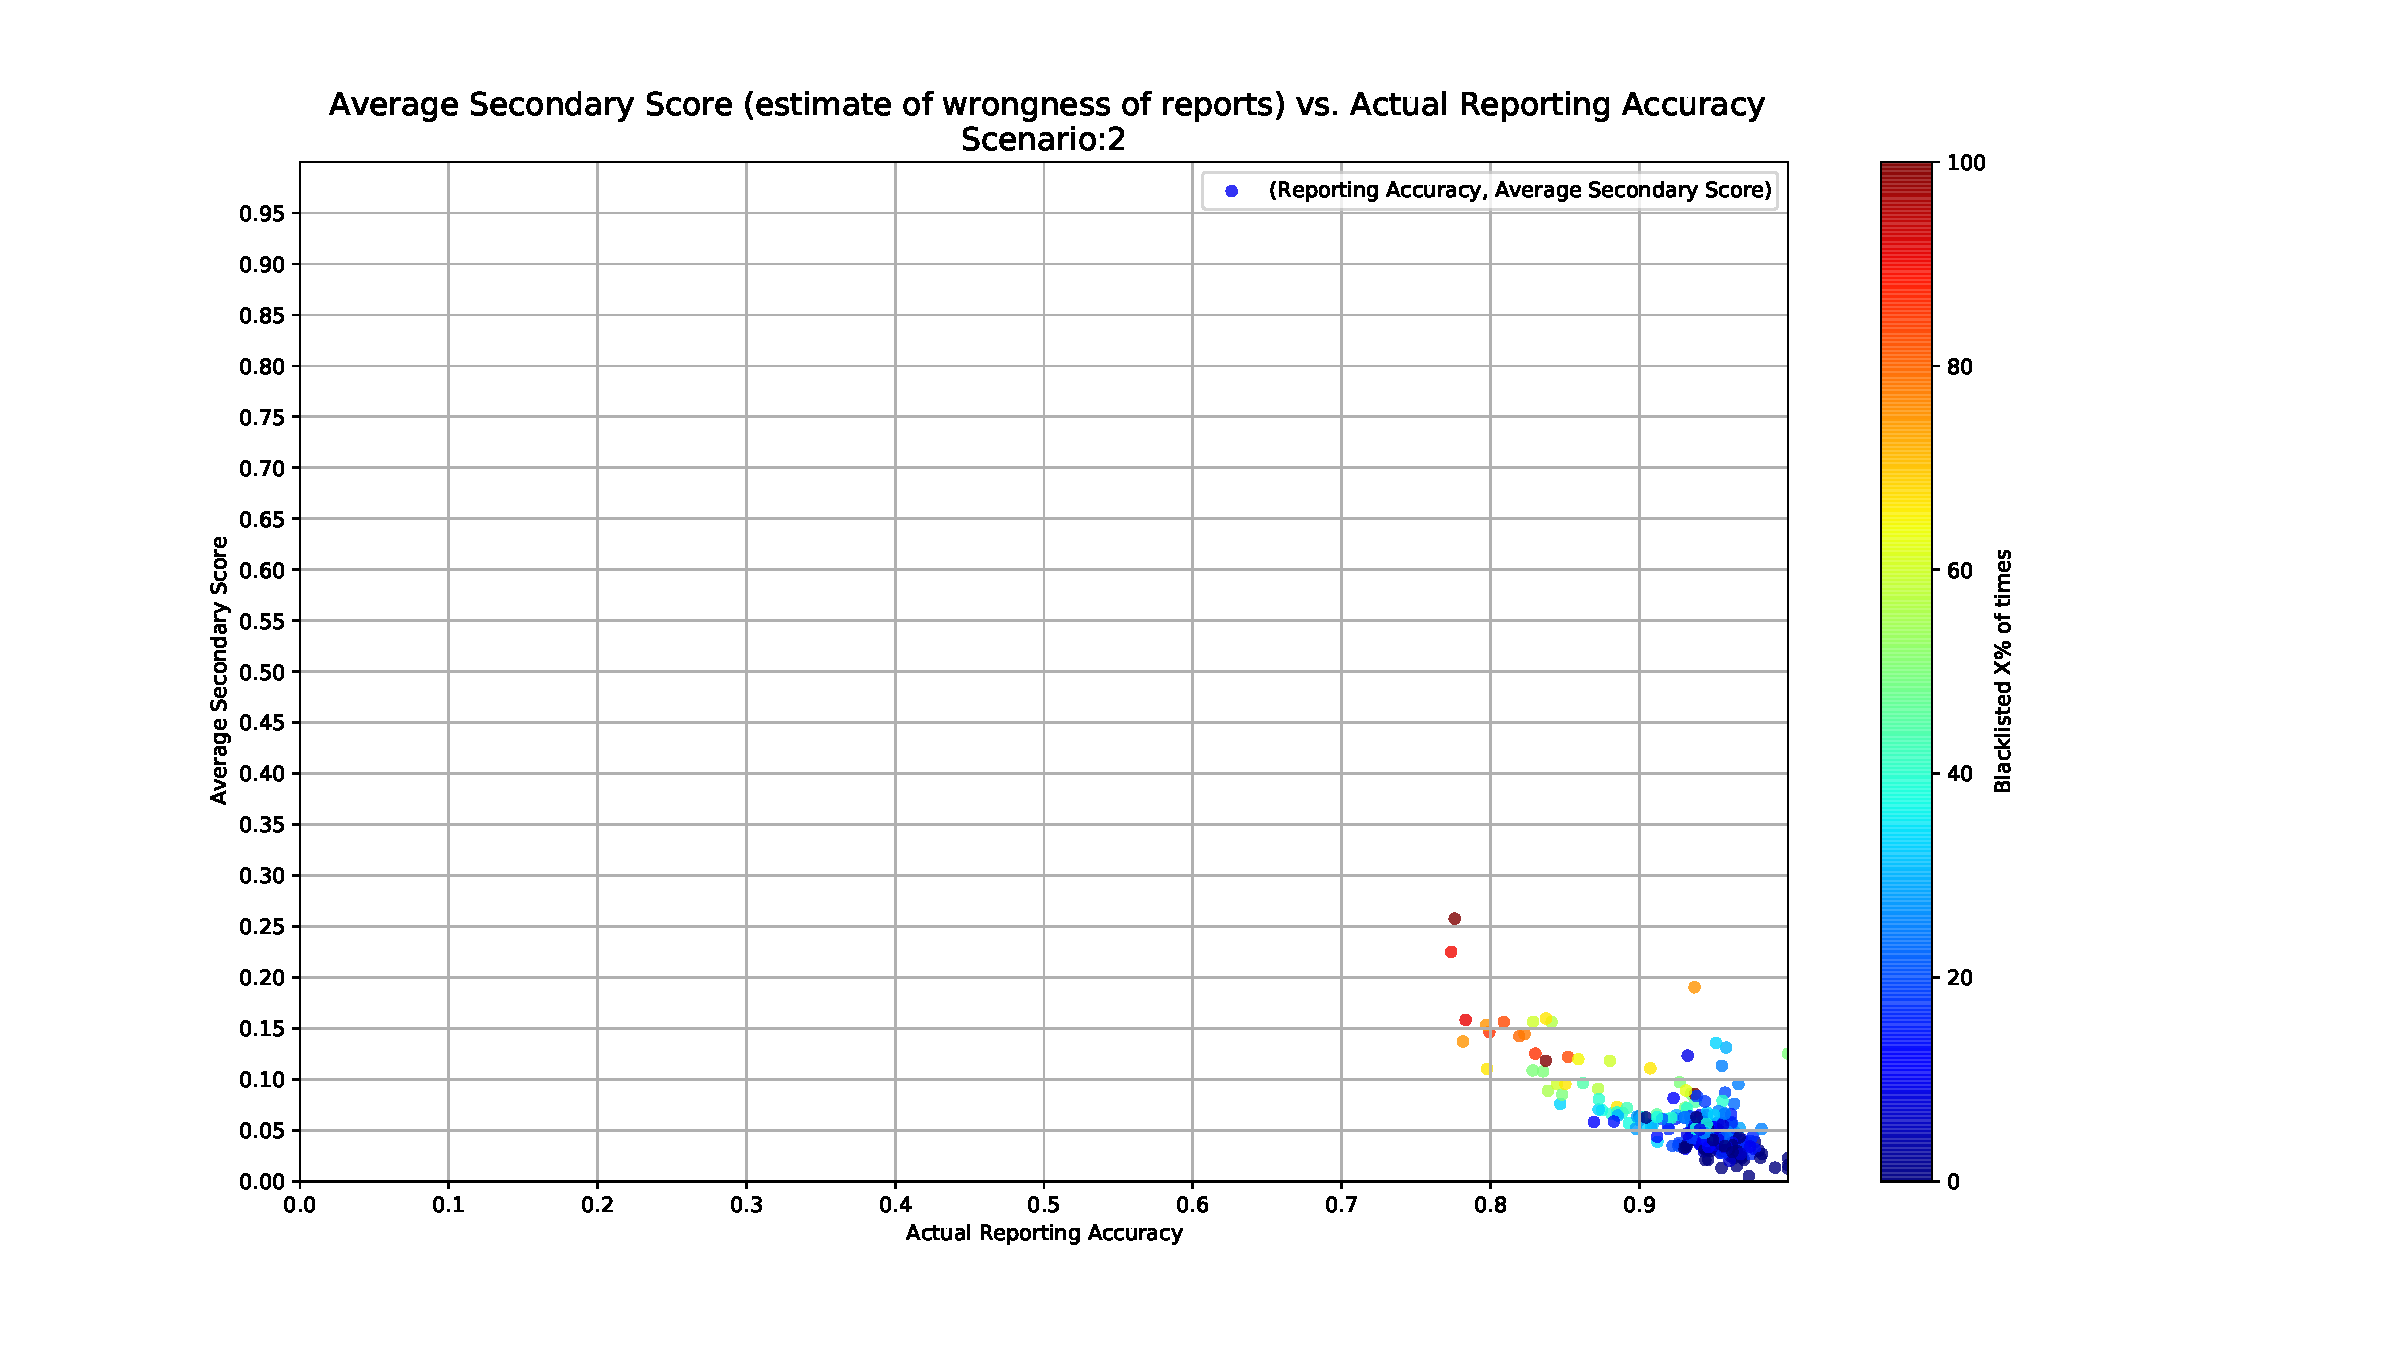
\includegraphics[width=0.5\linewidth,trim={100 50 185 72}, clip]{images/SCN2_ReportingAccuracy_Vs_AvgSecondaryScore.pdf}
		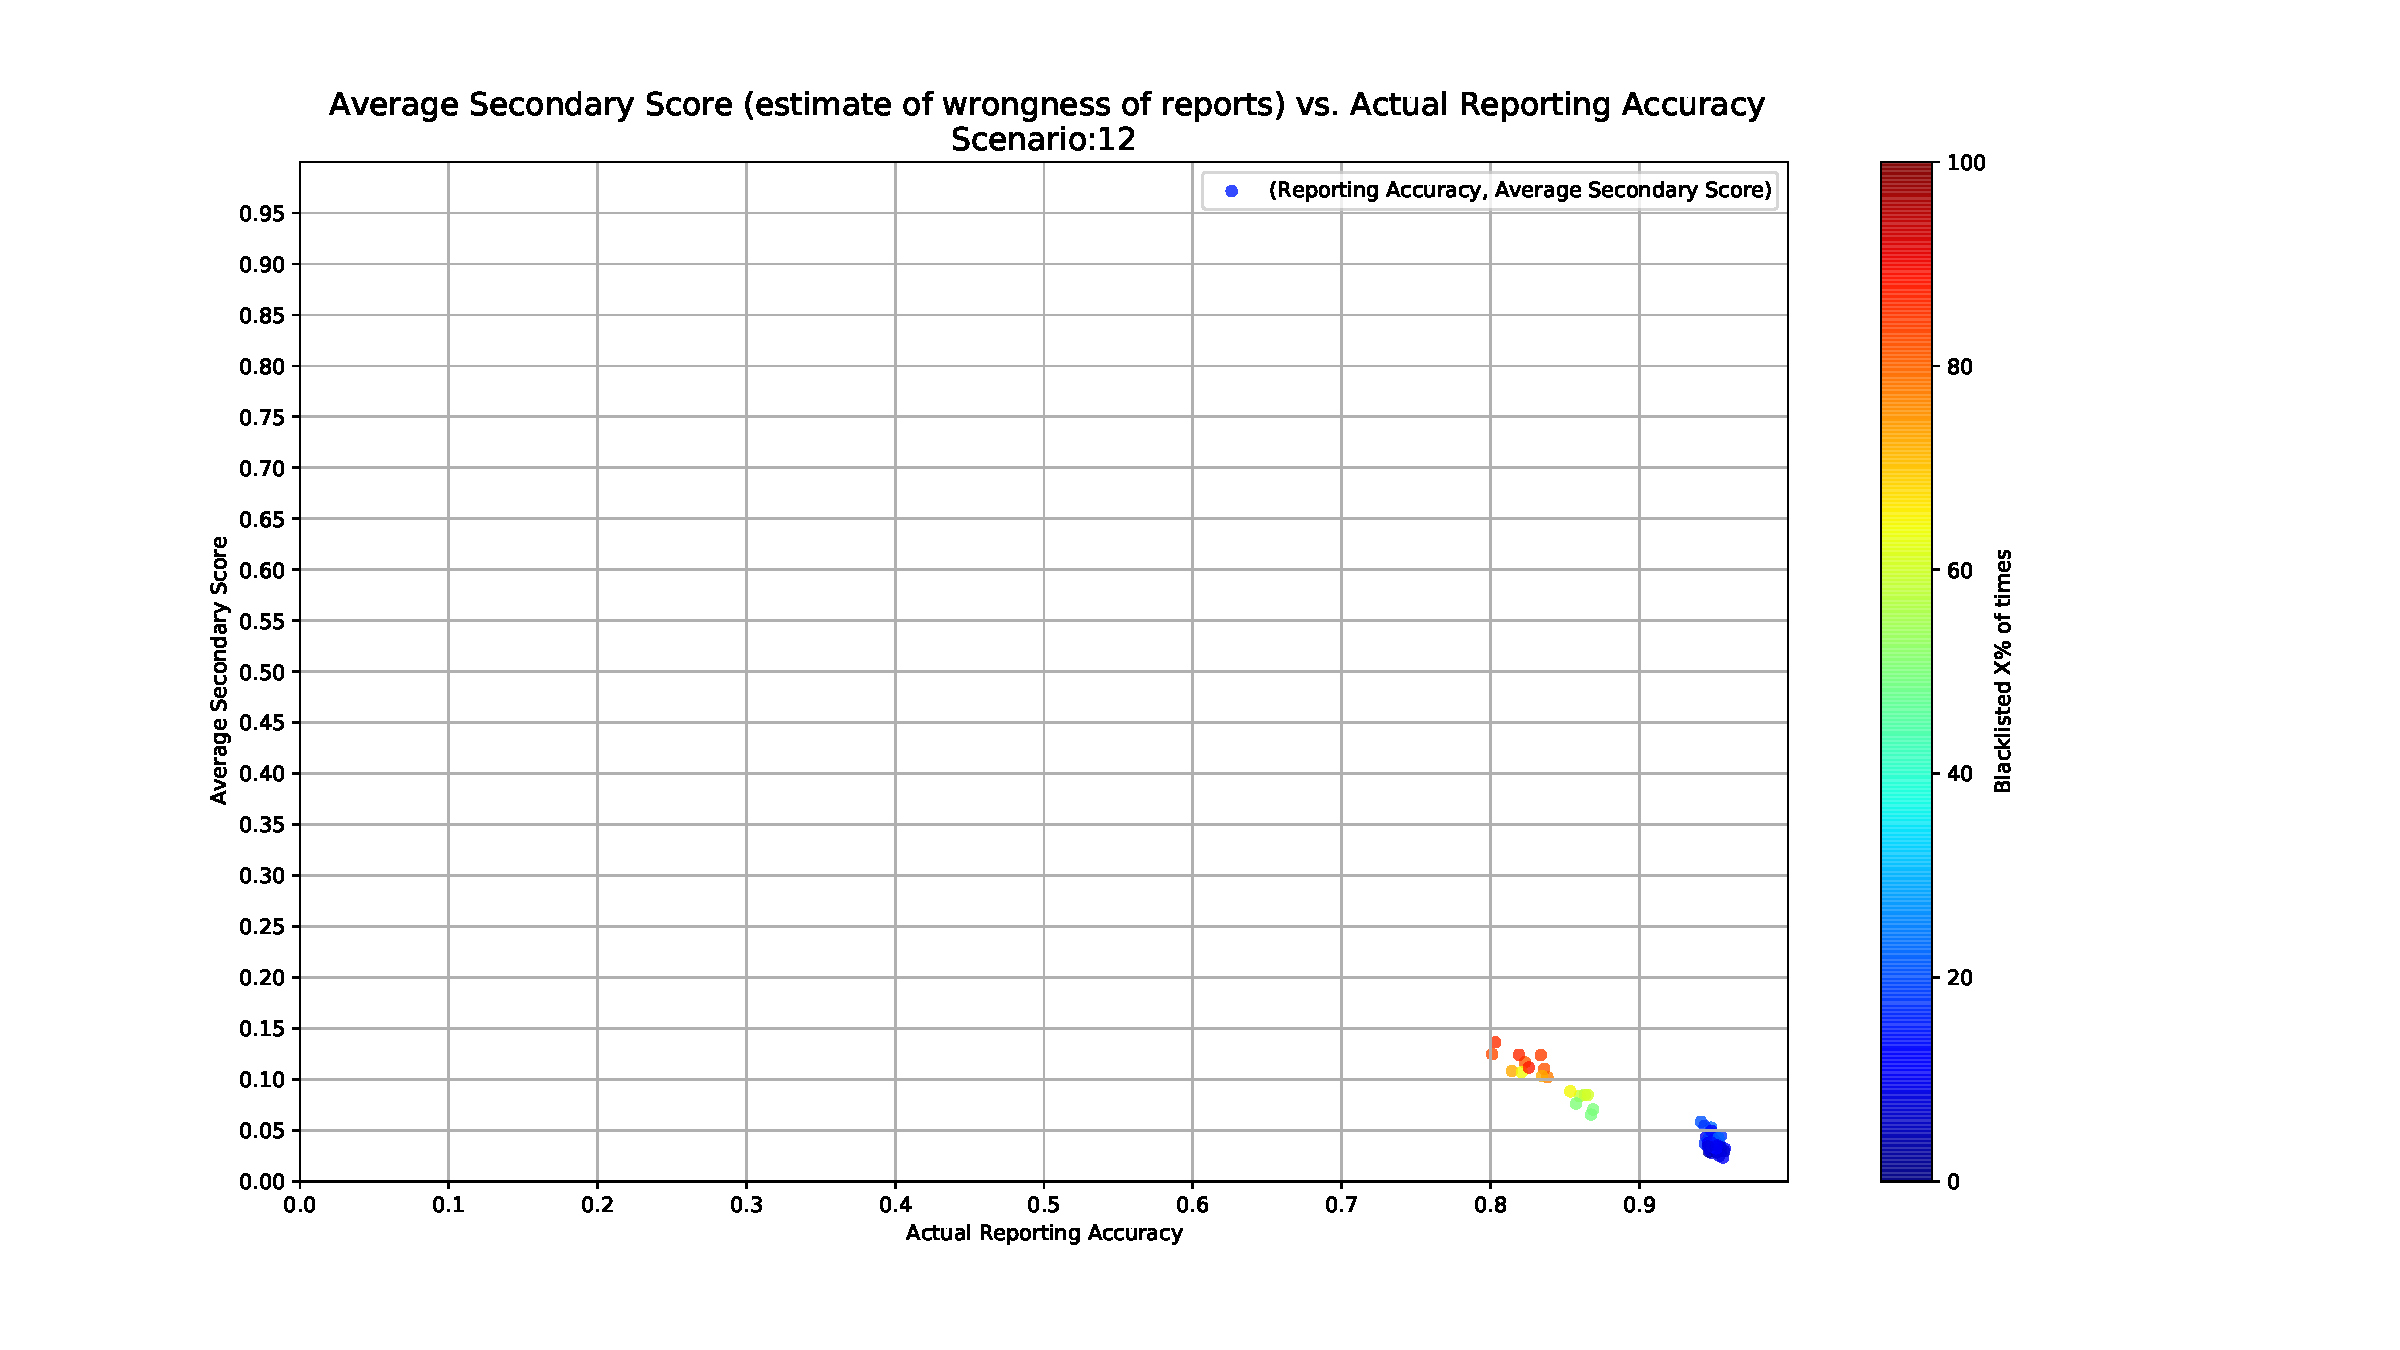
\includegraphics[width=0.5\linewidth,trim={100 50 185 72}, clip]{images/SCN12_ReportingAccuracy_Vs_AvgSecondaryScore.pdf}
	}
\end{figure*}
\iffalse
\begin{figure*}[!ht]
	\caption{Graphs for Results of Scenario 0. (a) Primary Score vs. Actual Accuracy - Scatter plot. (b) Primary Score and Actual Accuracy KDE. An Indicator of closeness of estimates. (c) Absolute error (difference between actual accuracy of node and estimated accuracy) vs. Percentage of nodes for which there was less than 'x'\% error. (d) Mean Secondary Score vs. Accuracy of Reports Sent - Scatter plot.}
	\label{fig:apdx:sc0}
	\centering
	\subfloat[]{
		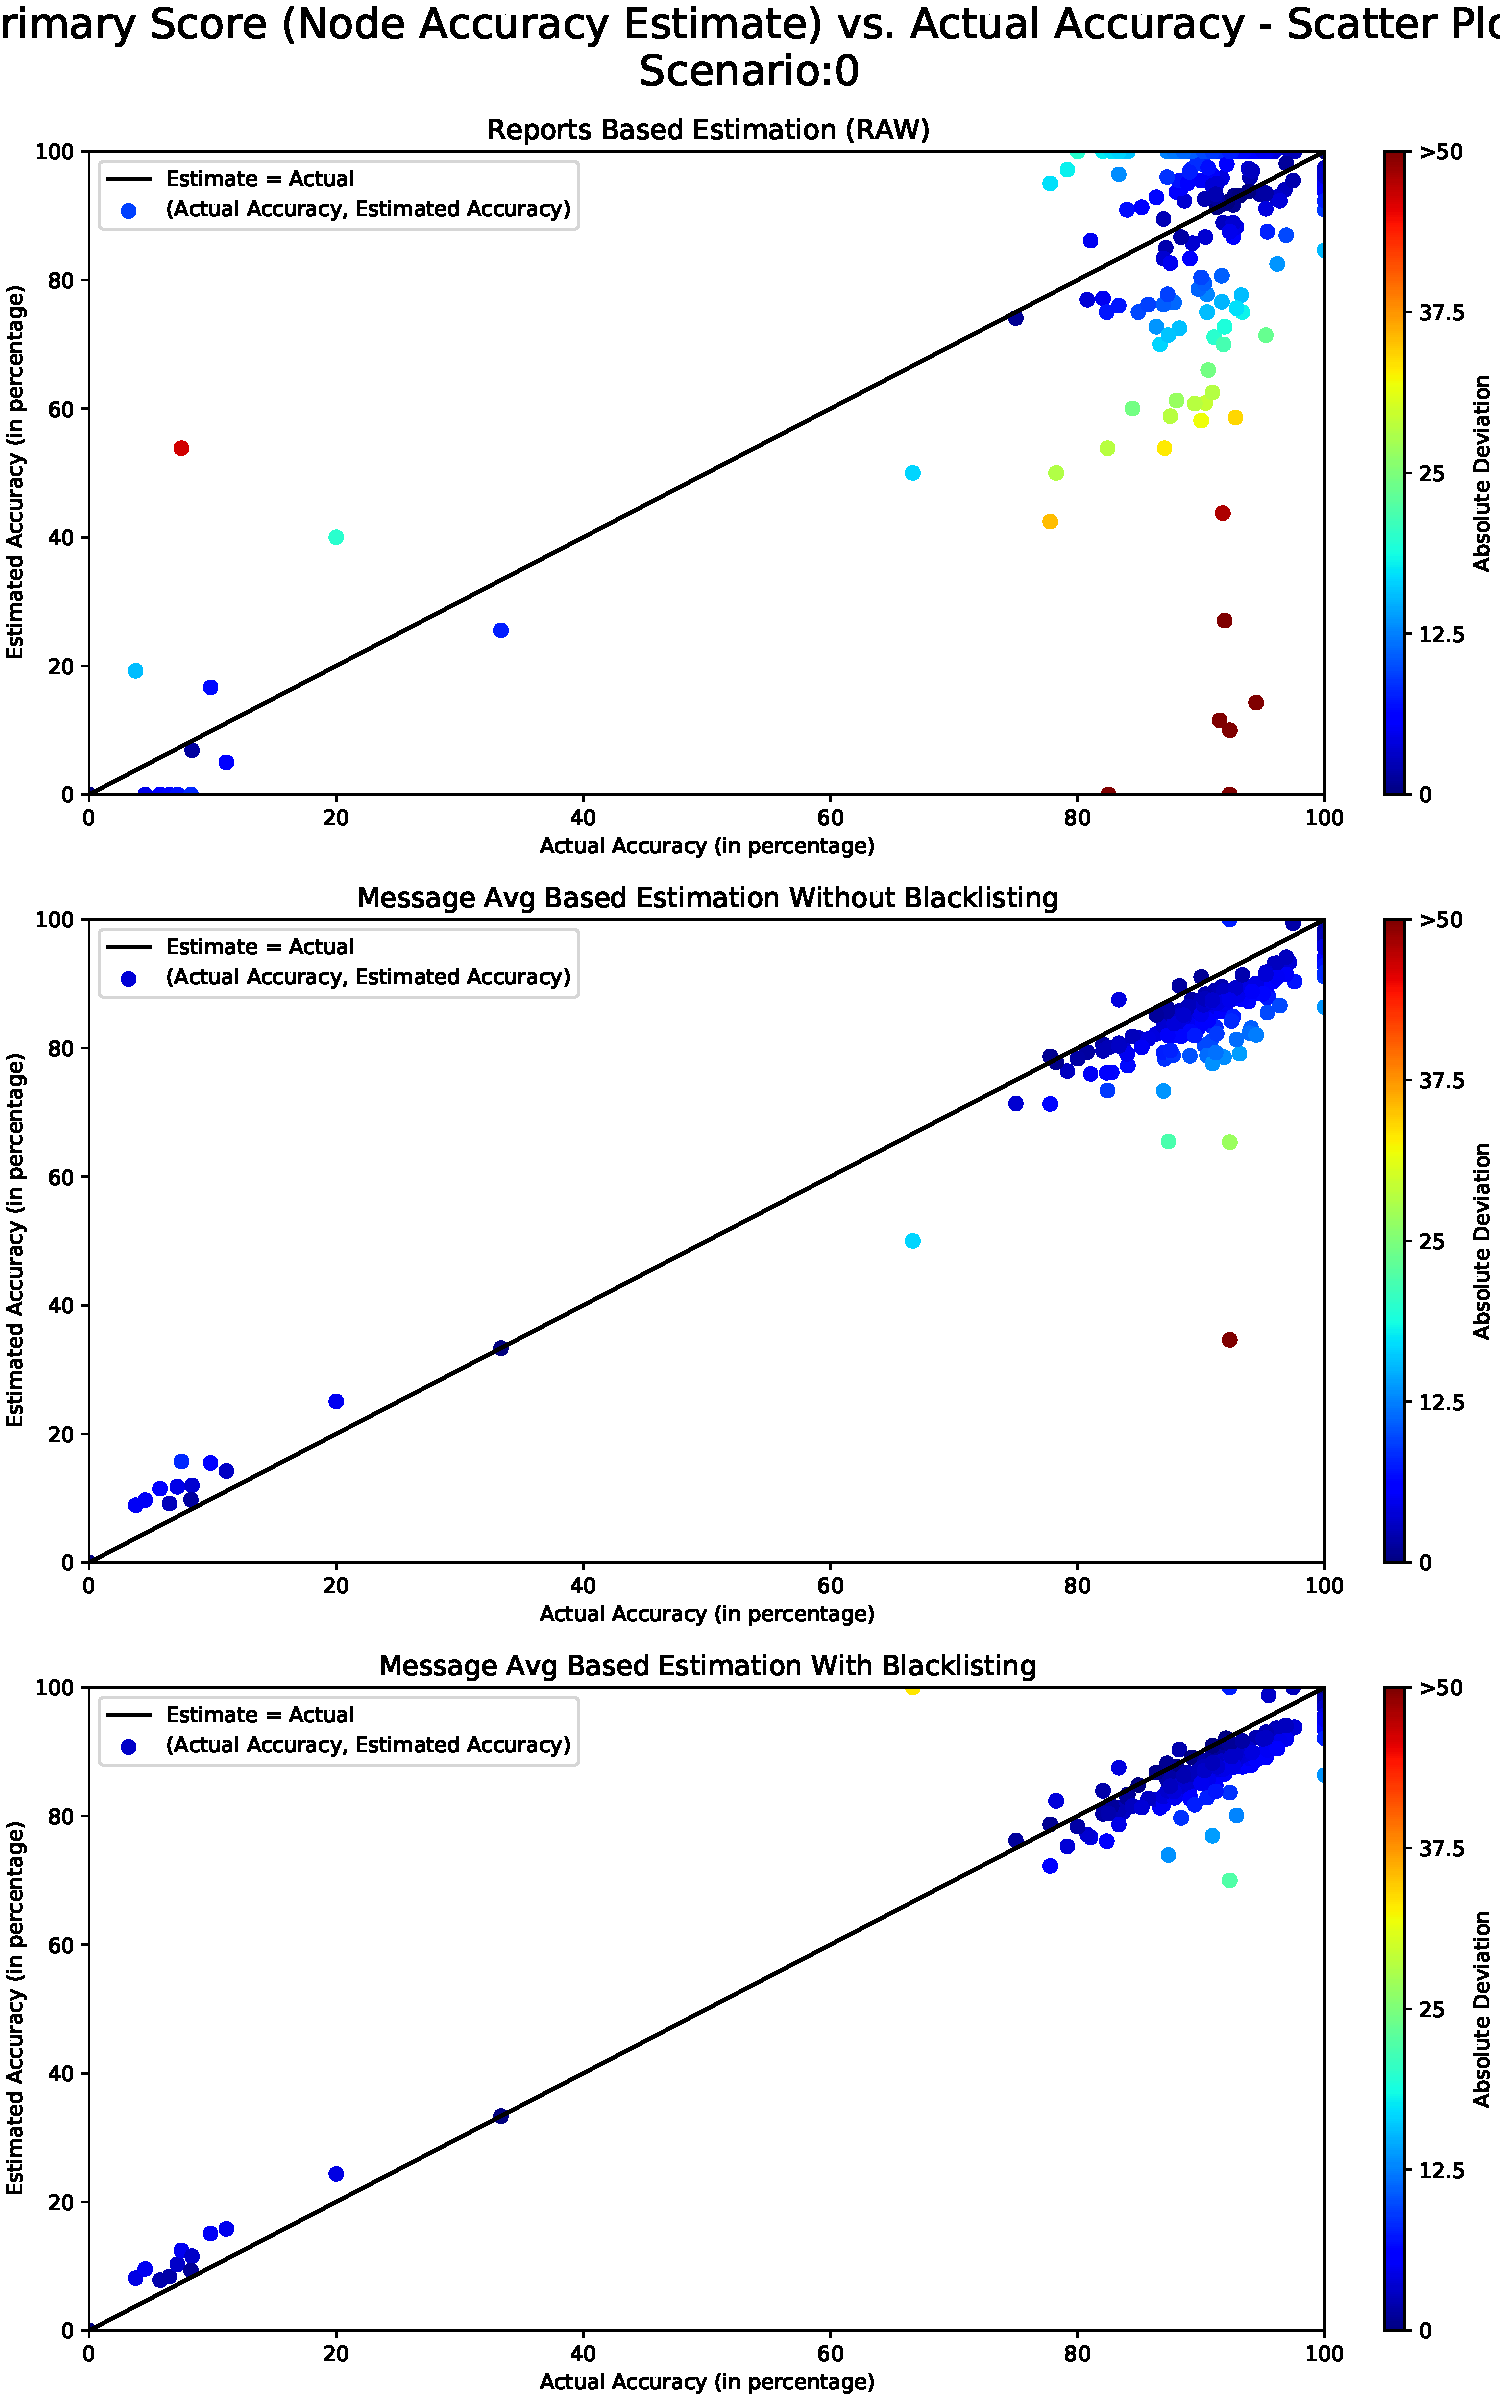
\includegraphics[width=0.5\linewidth, trim={0 5 15 50}, clip]{images/SCN0_PrimaryScoreVsActualAccuracyComparitive.pdf}
	}
	\subfloat[]{
		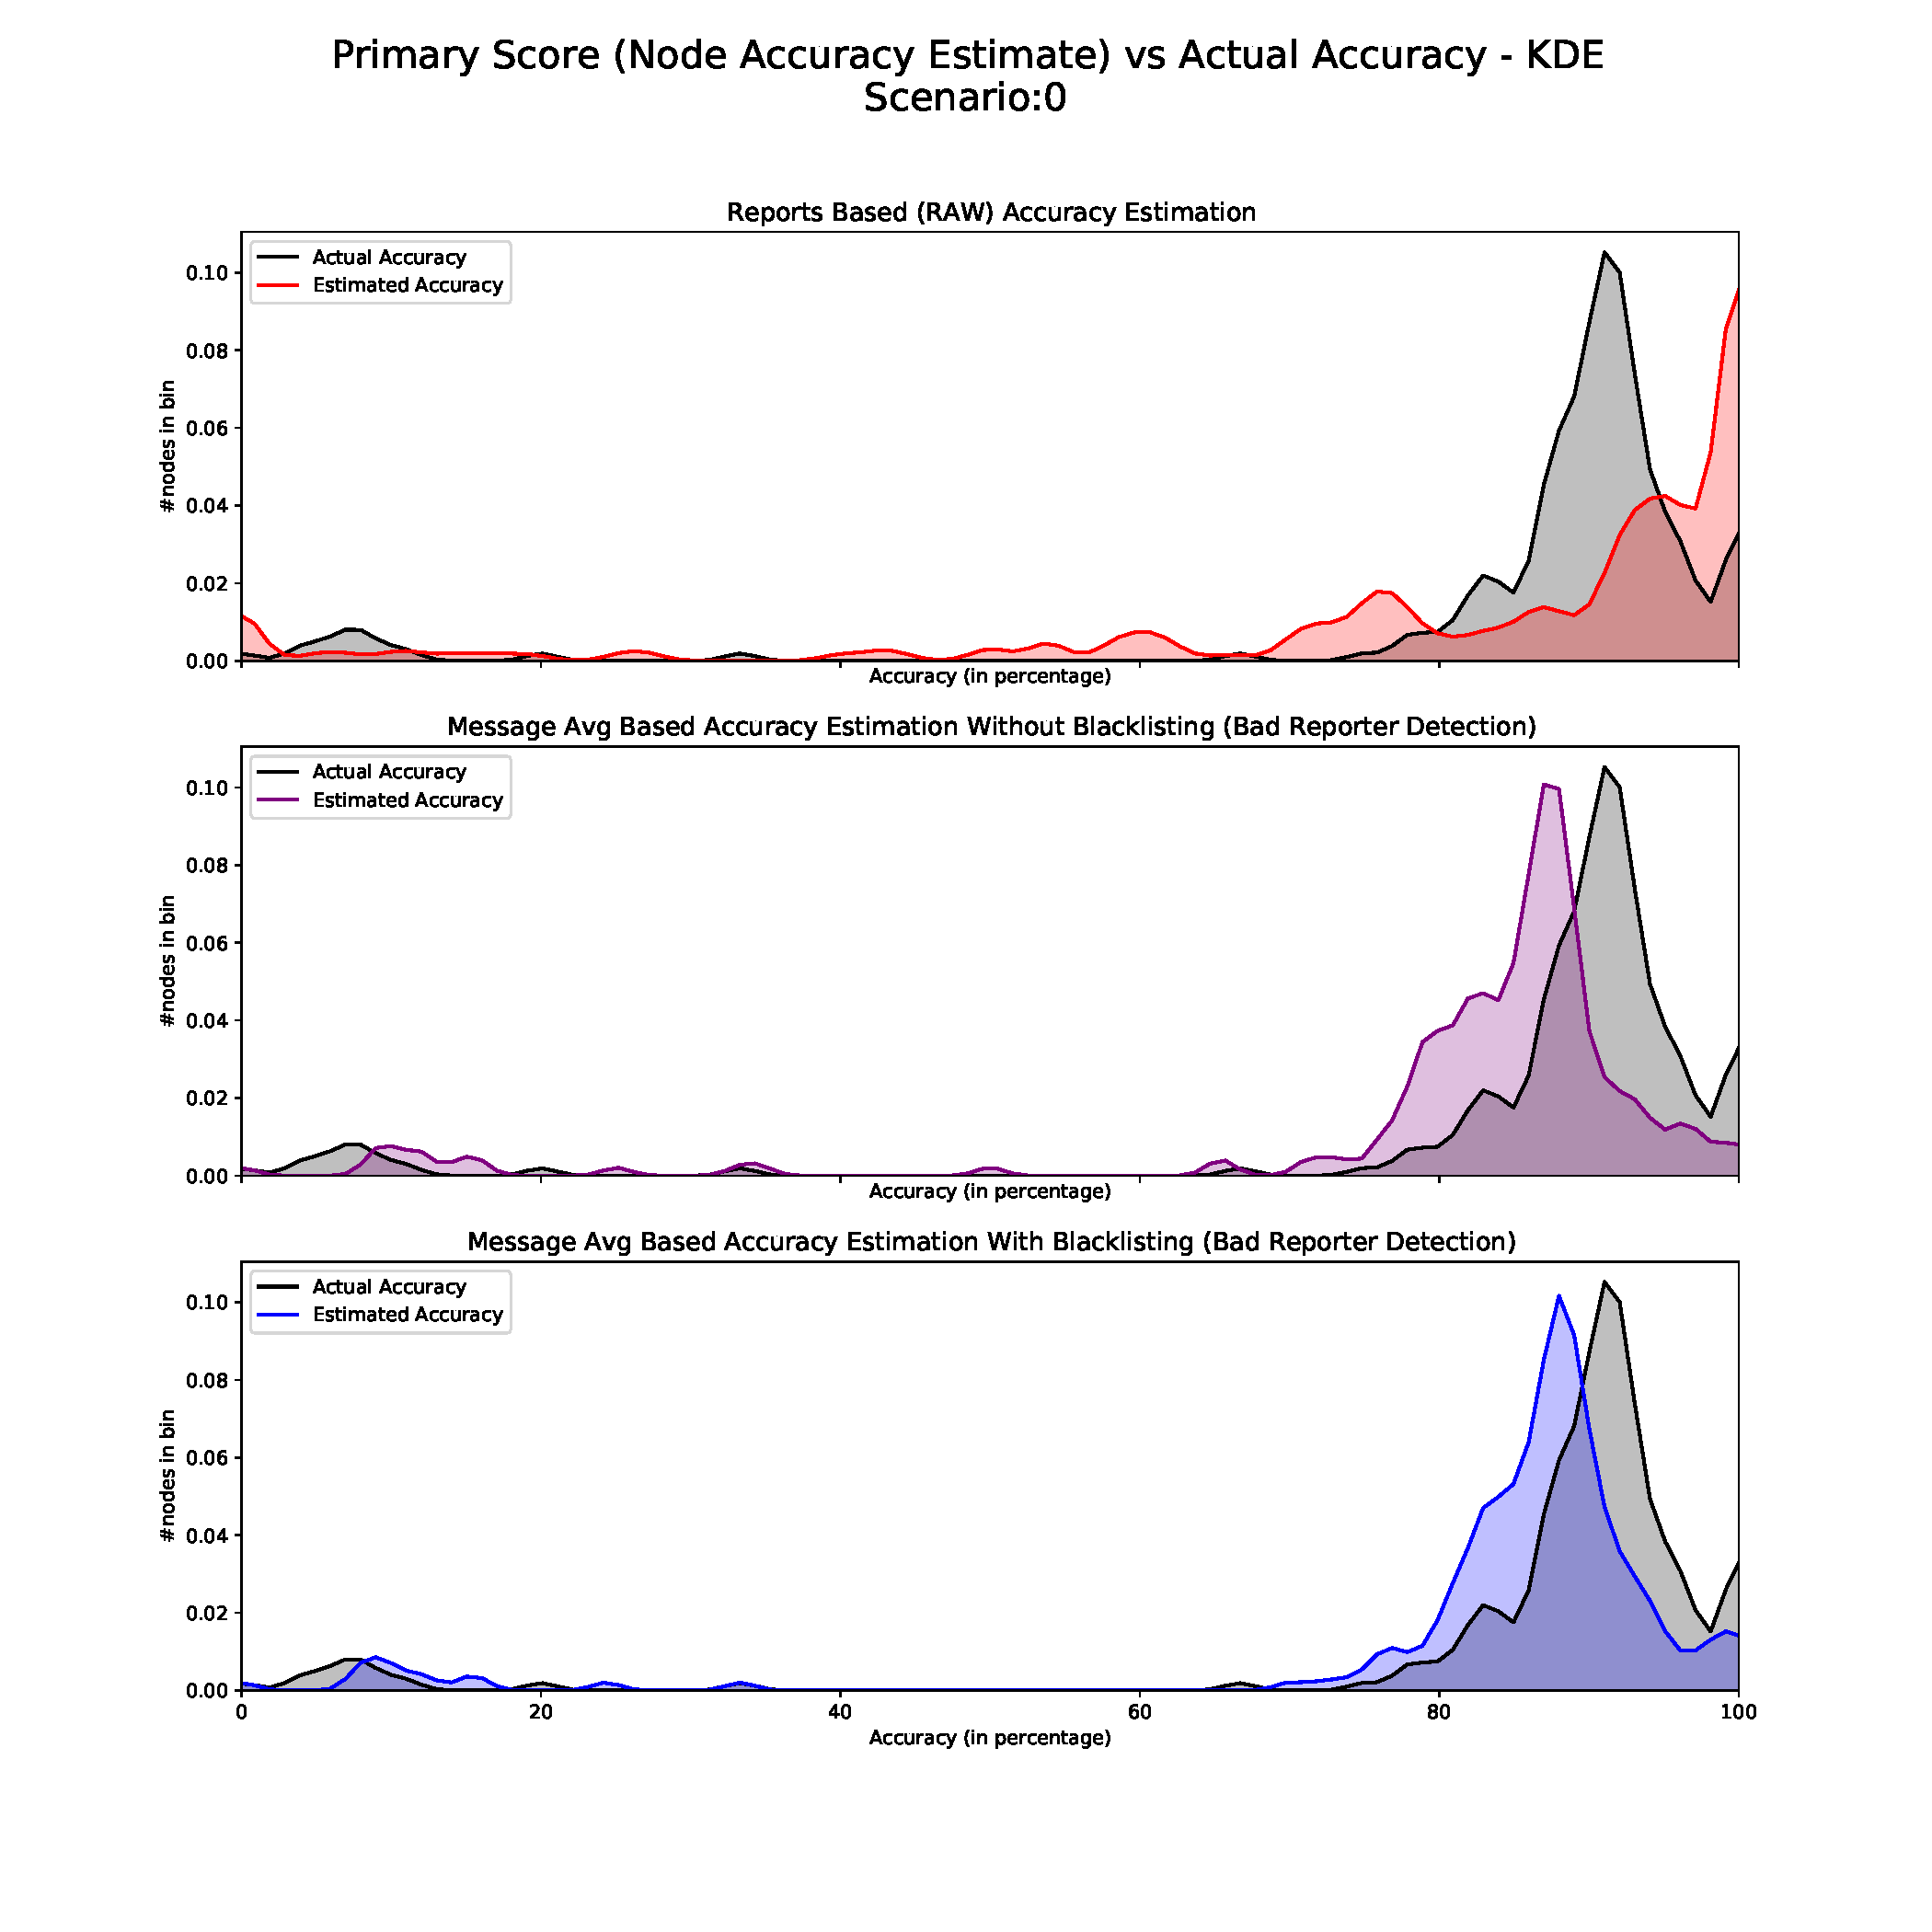
\includegraphics[width=0.5\linewidth, trim={80 95 100 100}, clip]{images/SCN0_PrimaryScoreKDEComparitive.pdf}
	}
	\hfill
	\subfloat[]{
		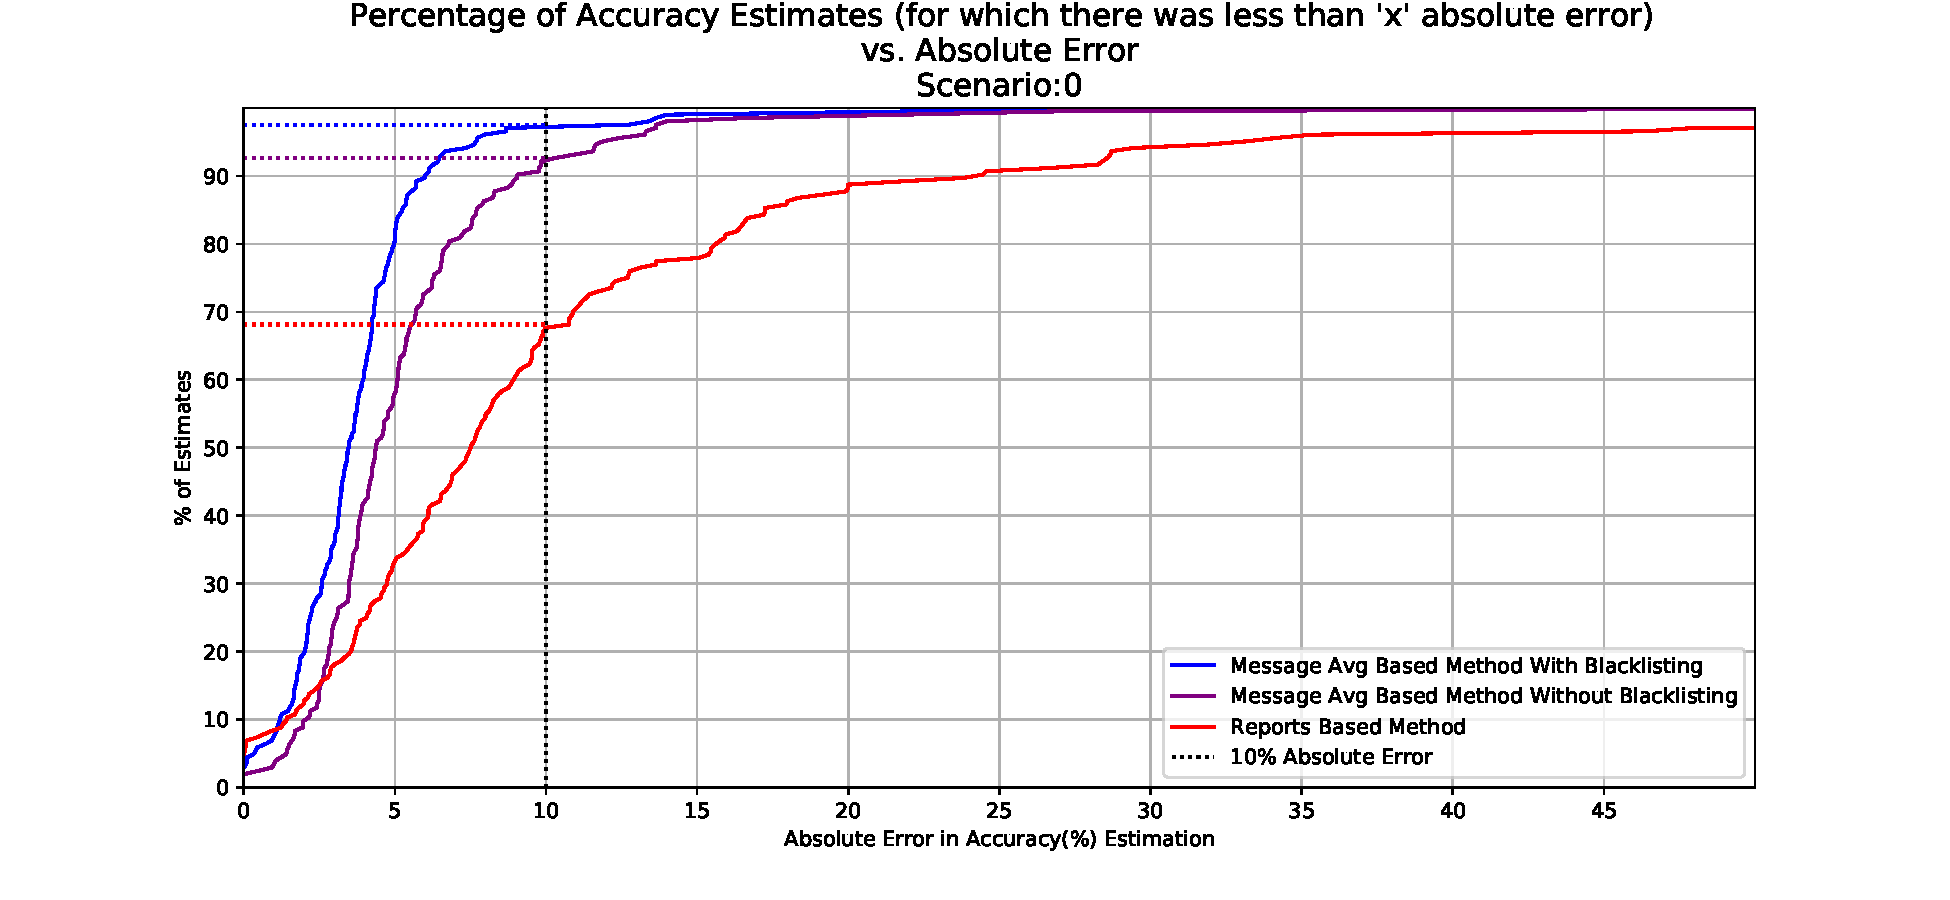
\includegraphics[width=0.5\linewidth, trim={80 25 90 50}, clip]{images/SCN0_AbsoluteErrorsInEstimationComparison.pdf}
	}
	\subfloat[]{
		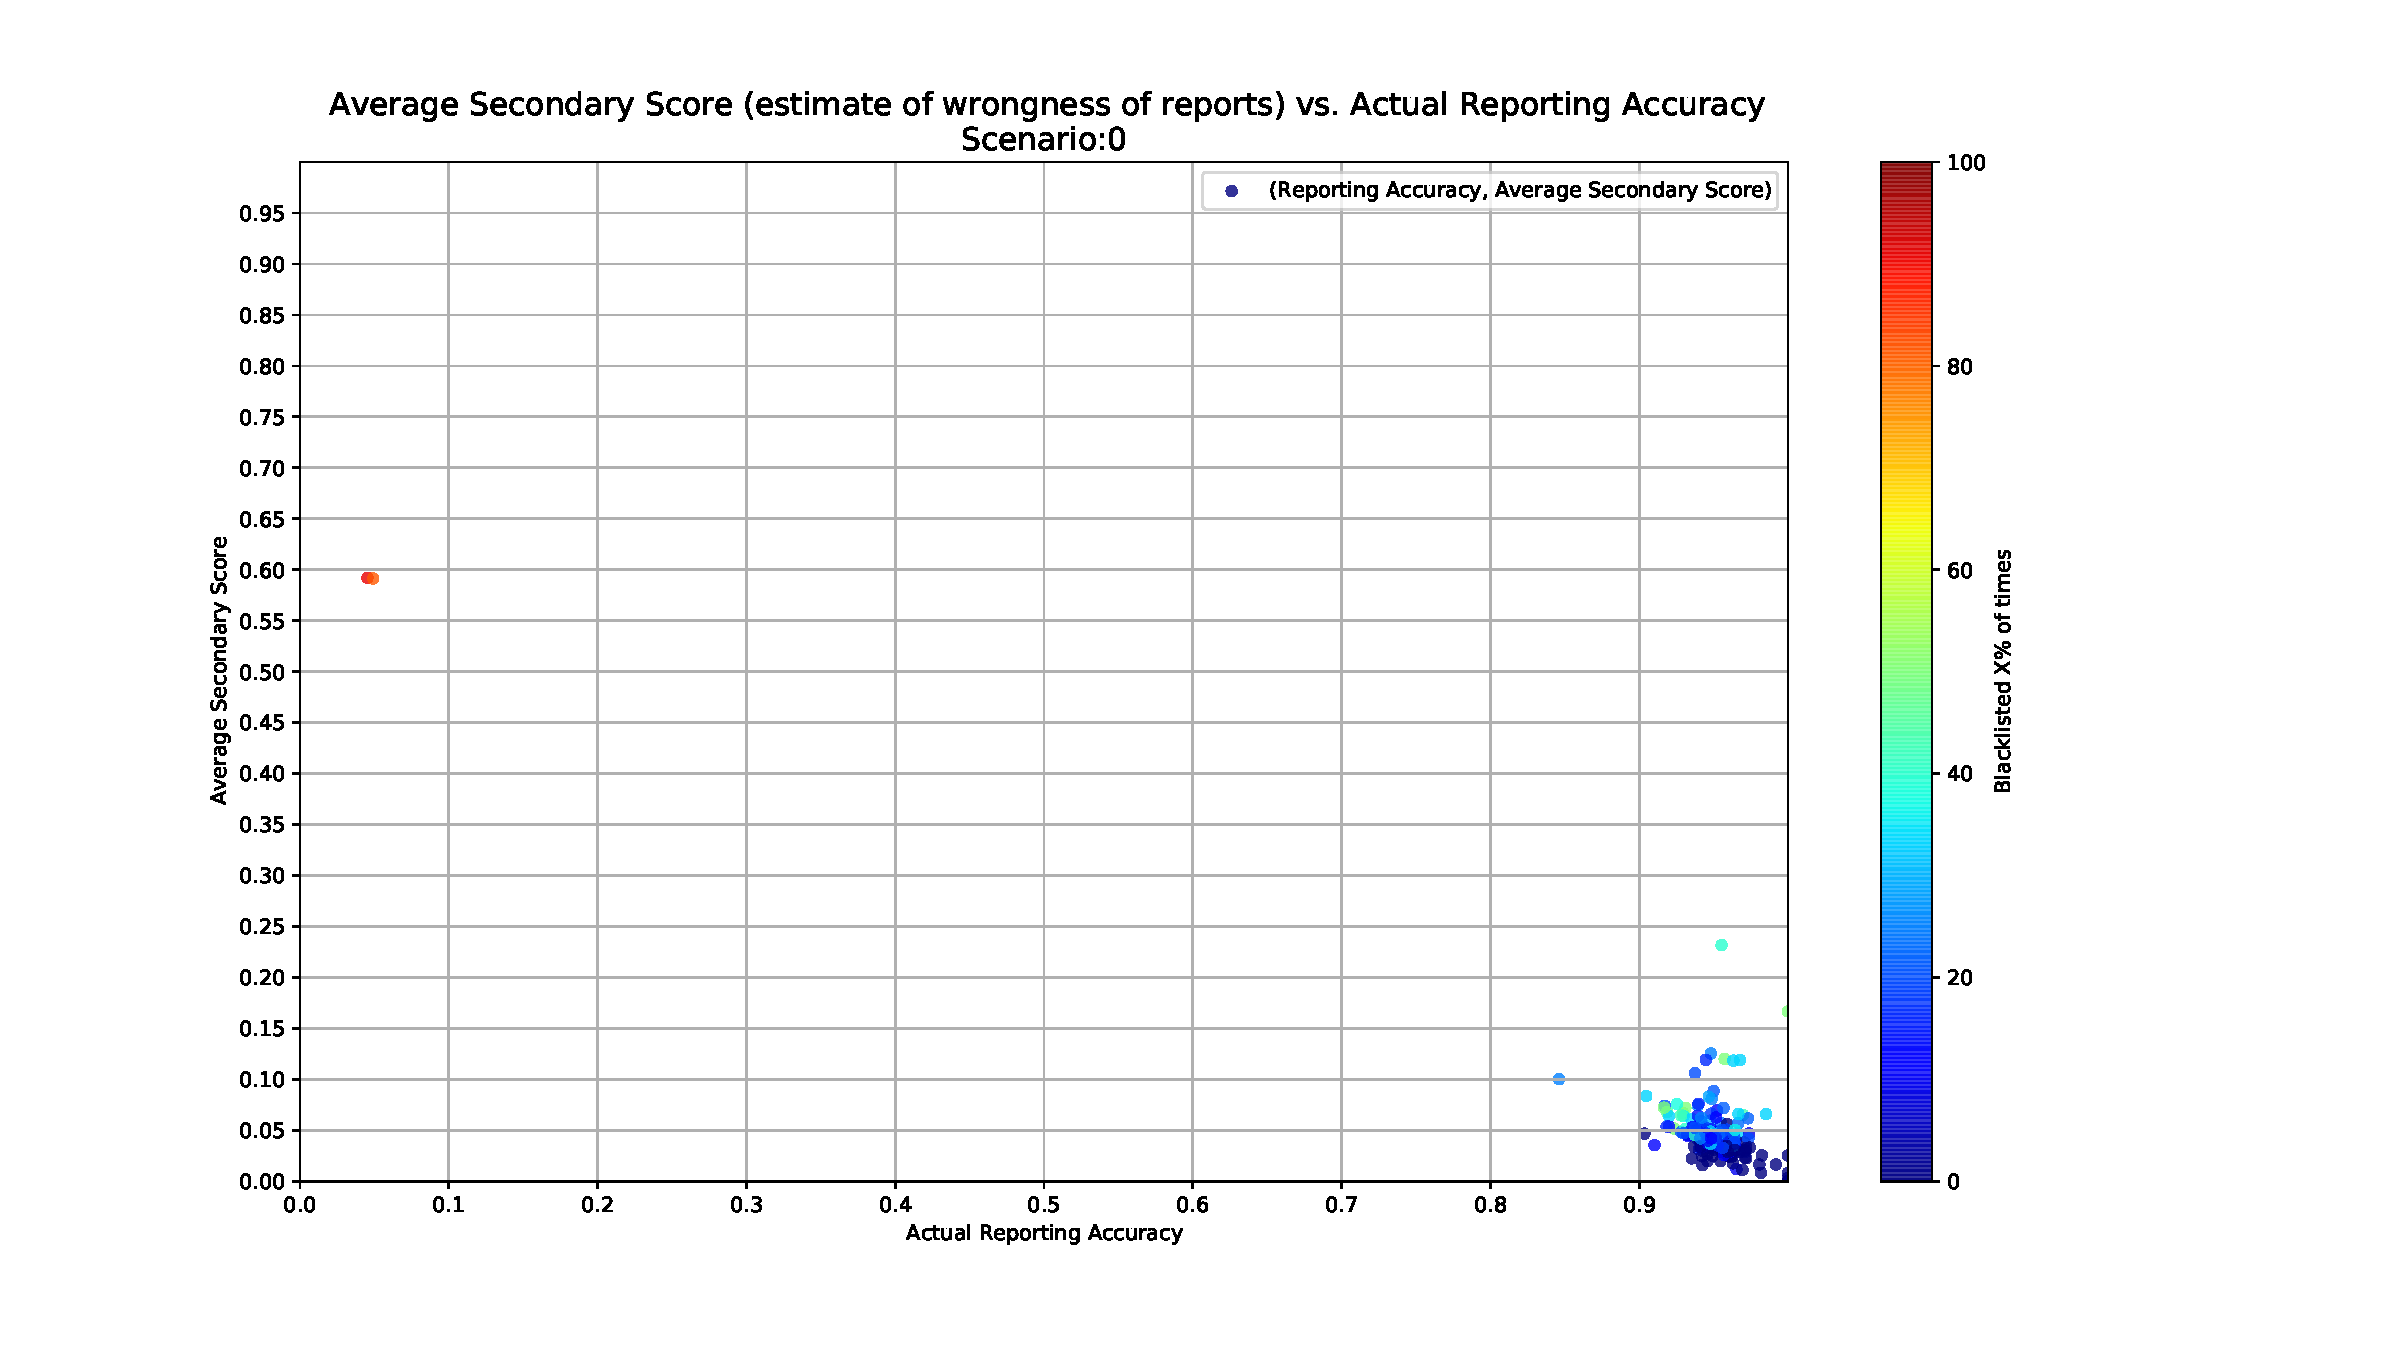
\includegraphics[width=0.5\linewidth,trim={100 50 185 72}, clip]{images/SCN0_ReportingAccuracy_Vs_AvgSecondaryScore.pdf}
	}
\end{figure*}
\begin{figure*}[!ht]
	\caption{Graphs for Results of Scenario 1). (a) Primary Score vs. Actual Accuracy - Scatter plot. (b) Primary Score and Actual Accuracy KDE. An Indicator of closeness of estimates. (c) Absolute error (difference between actual accuracy of node and estimated accuracy) vs. Percentage of nodes for which there was less than 'x'\% error. (d) Mean Secondary Score vs. Accuracy of Reports Sent - Scatter plot.}
	\label{fig:apdx:sc1}
	\centering
	\subfloat[]{
		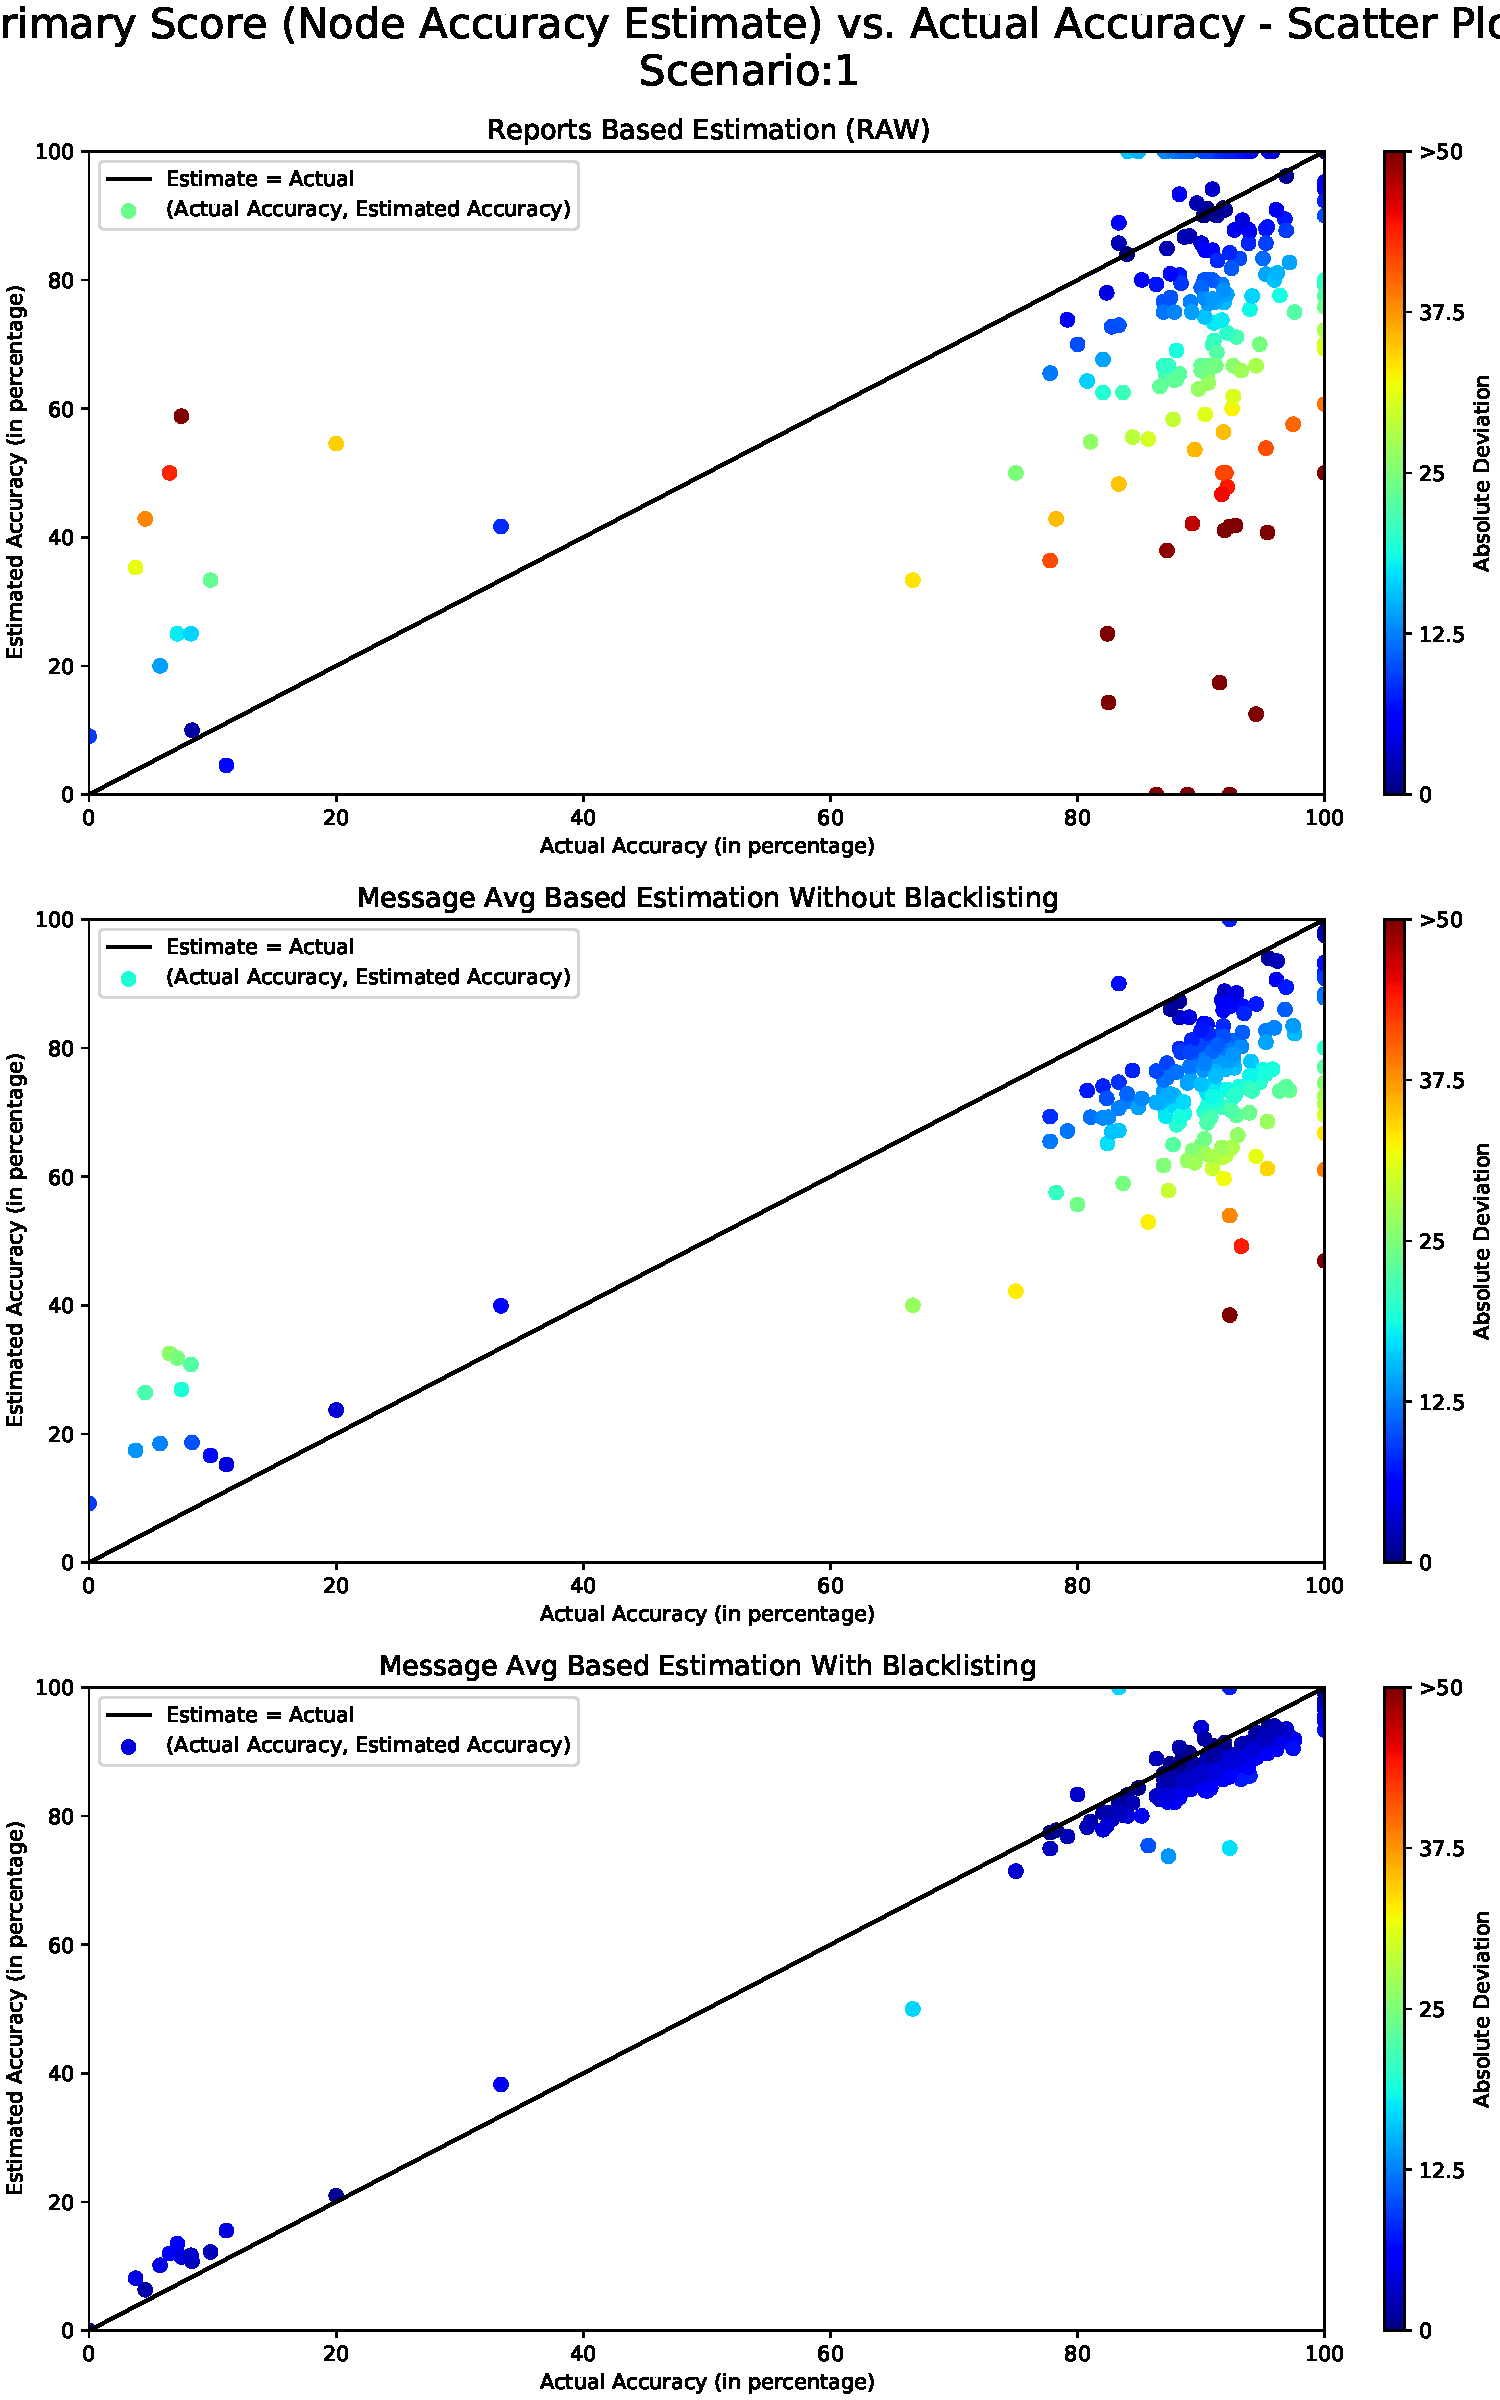
\includegraphics[width=0.5\linewidth, trim={0 5 15 50}, clip]{images/SCN1_PrimaryScoreVsActualAccuracyComparitive.pdf}
		\label{fig_first_case}
	}
	\subfloat[]{
		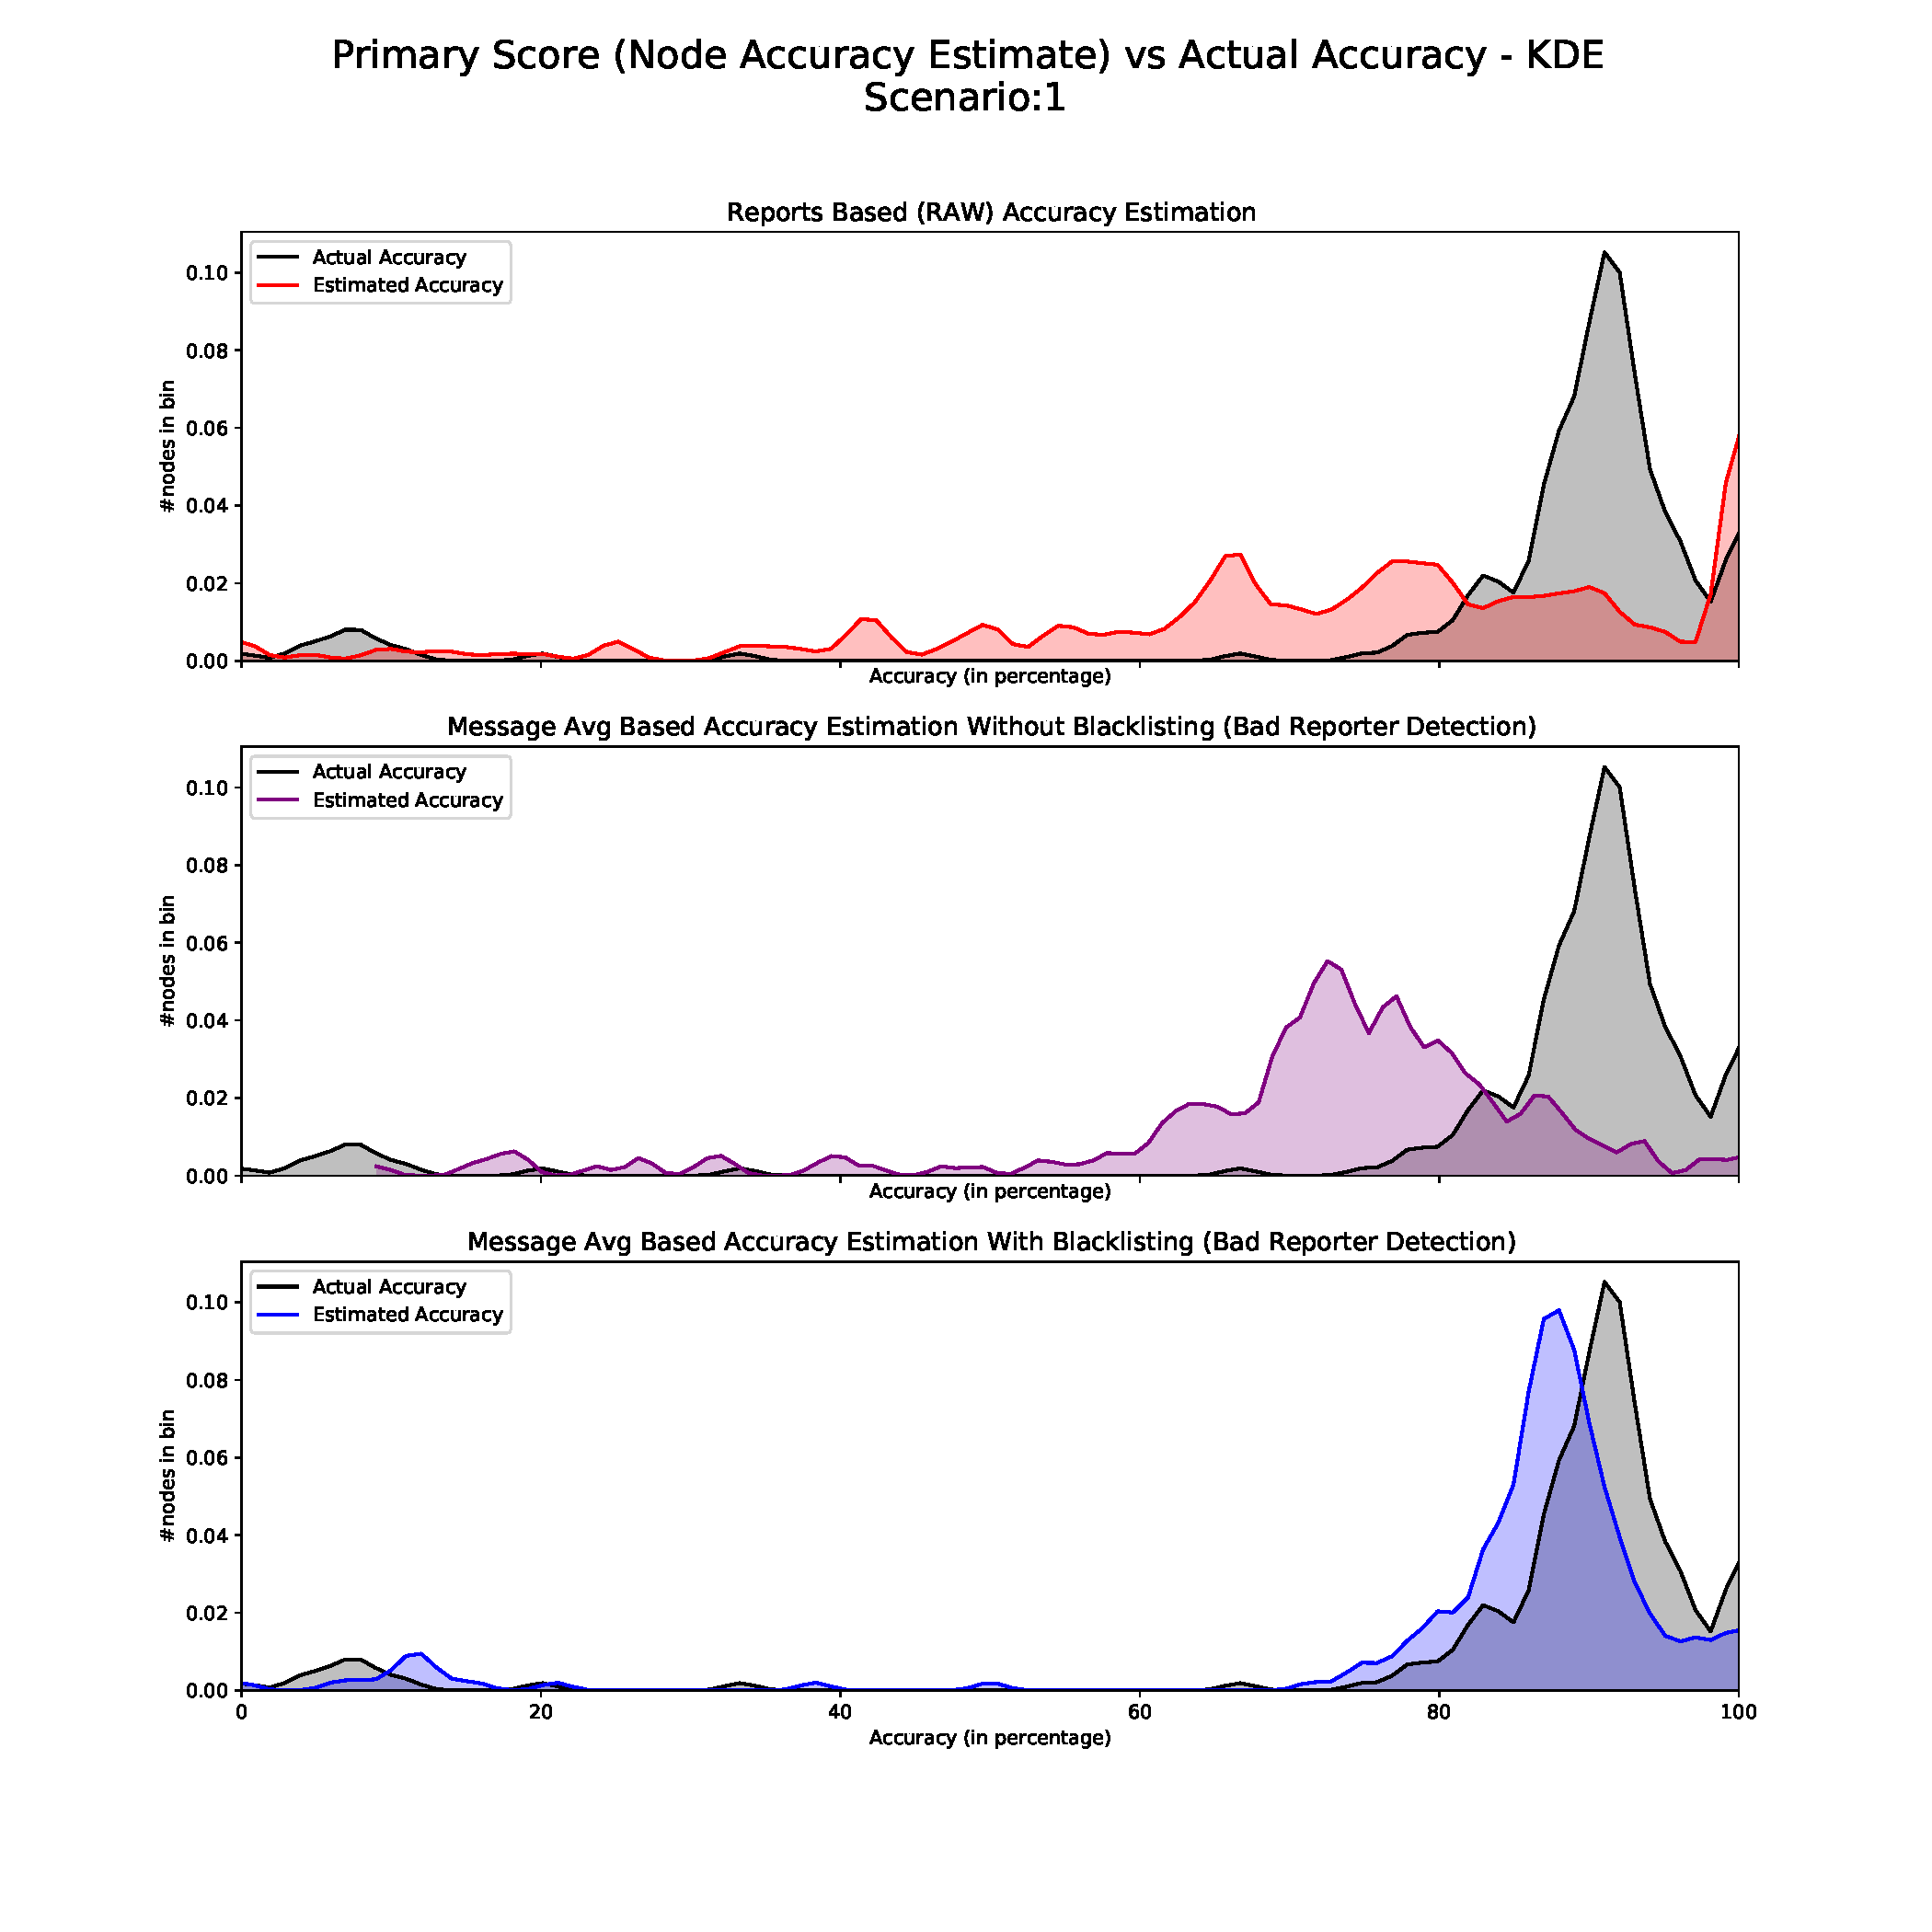
\includegraphics[width=0.5\linewidth, trim={80 95 100 100}, clip]{images/SCN1_PrimaryScoreKDEComparitive.pdf}
	}
	\hfill
	\subfloat[]{
		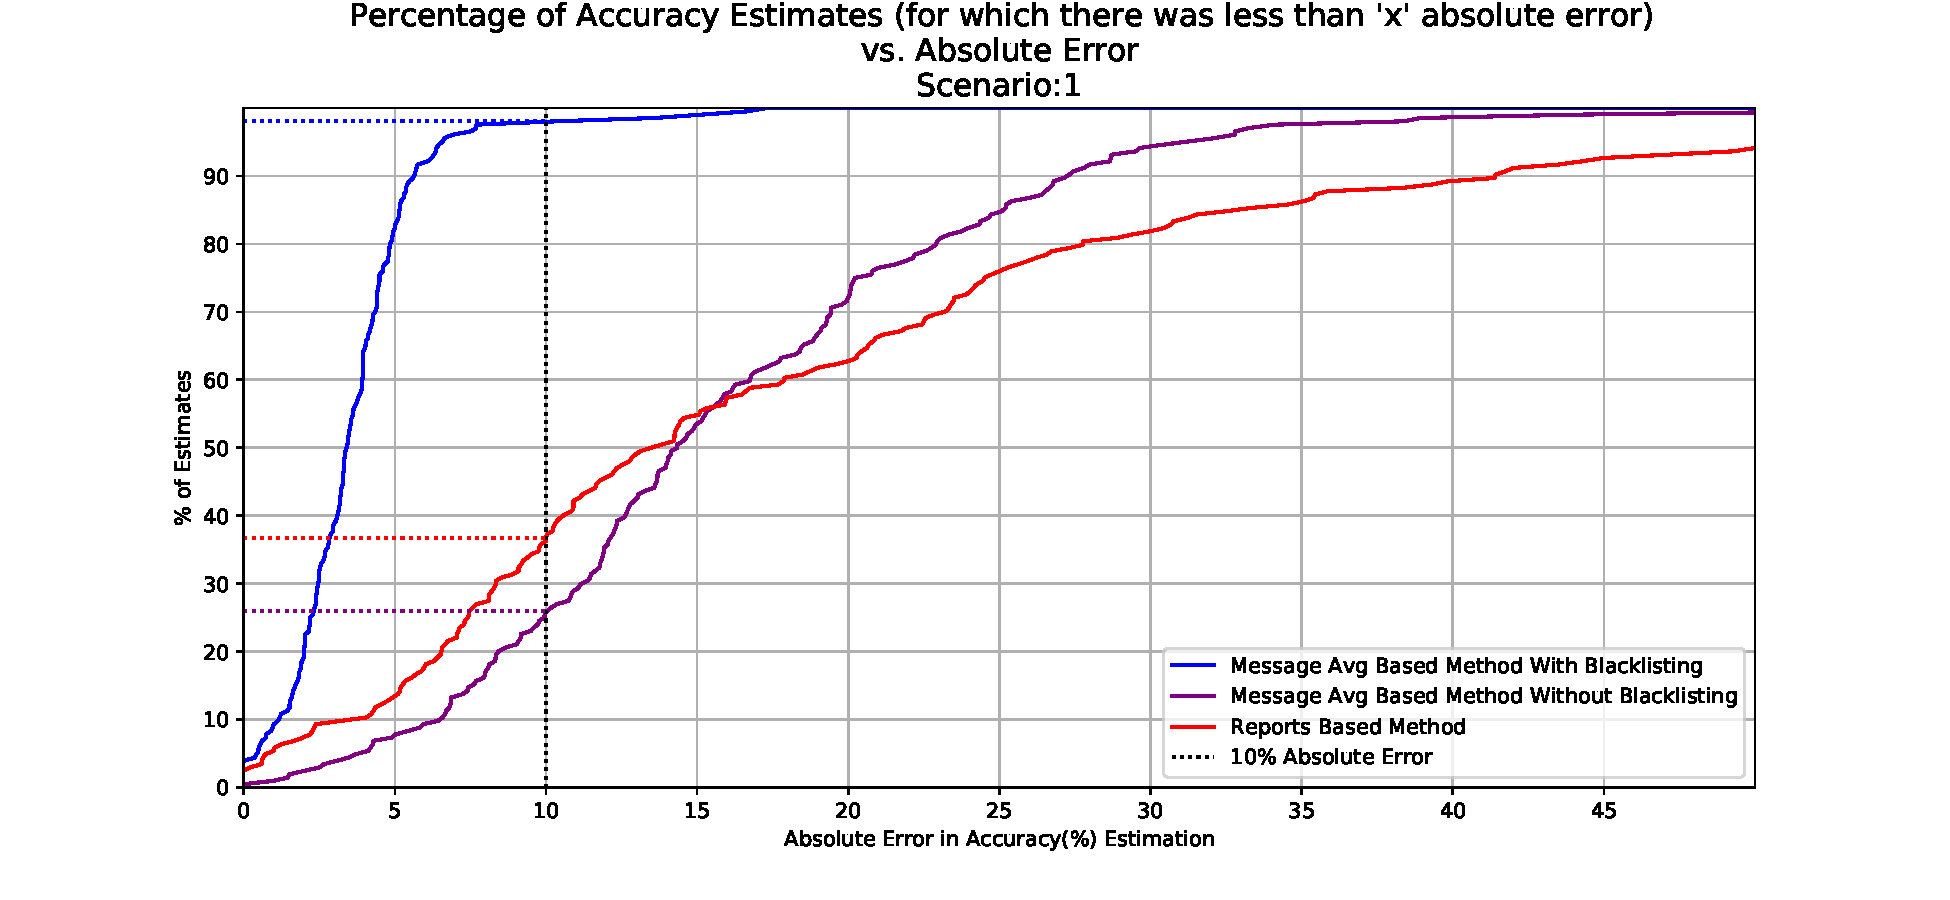
\includegraphics[width=0.5\linewidth, trim={80 25 90 50}, clip]{images/SCN1_AbsoluteErrorsInEstimationComparison.pdf}
	}
	\subfloat[]{
		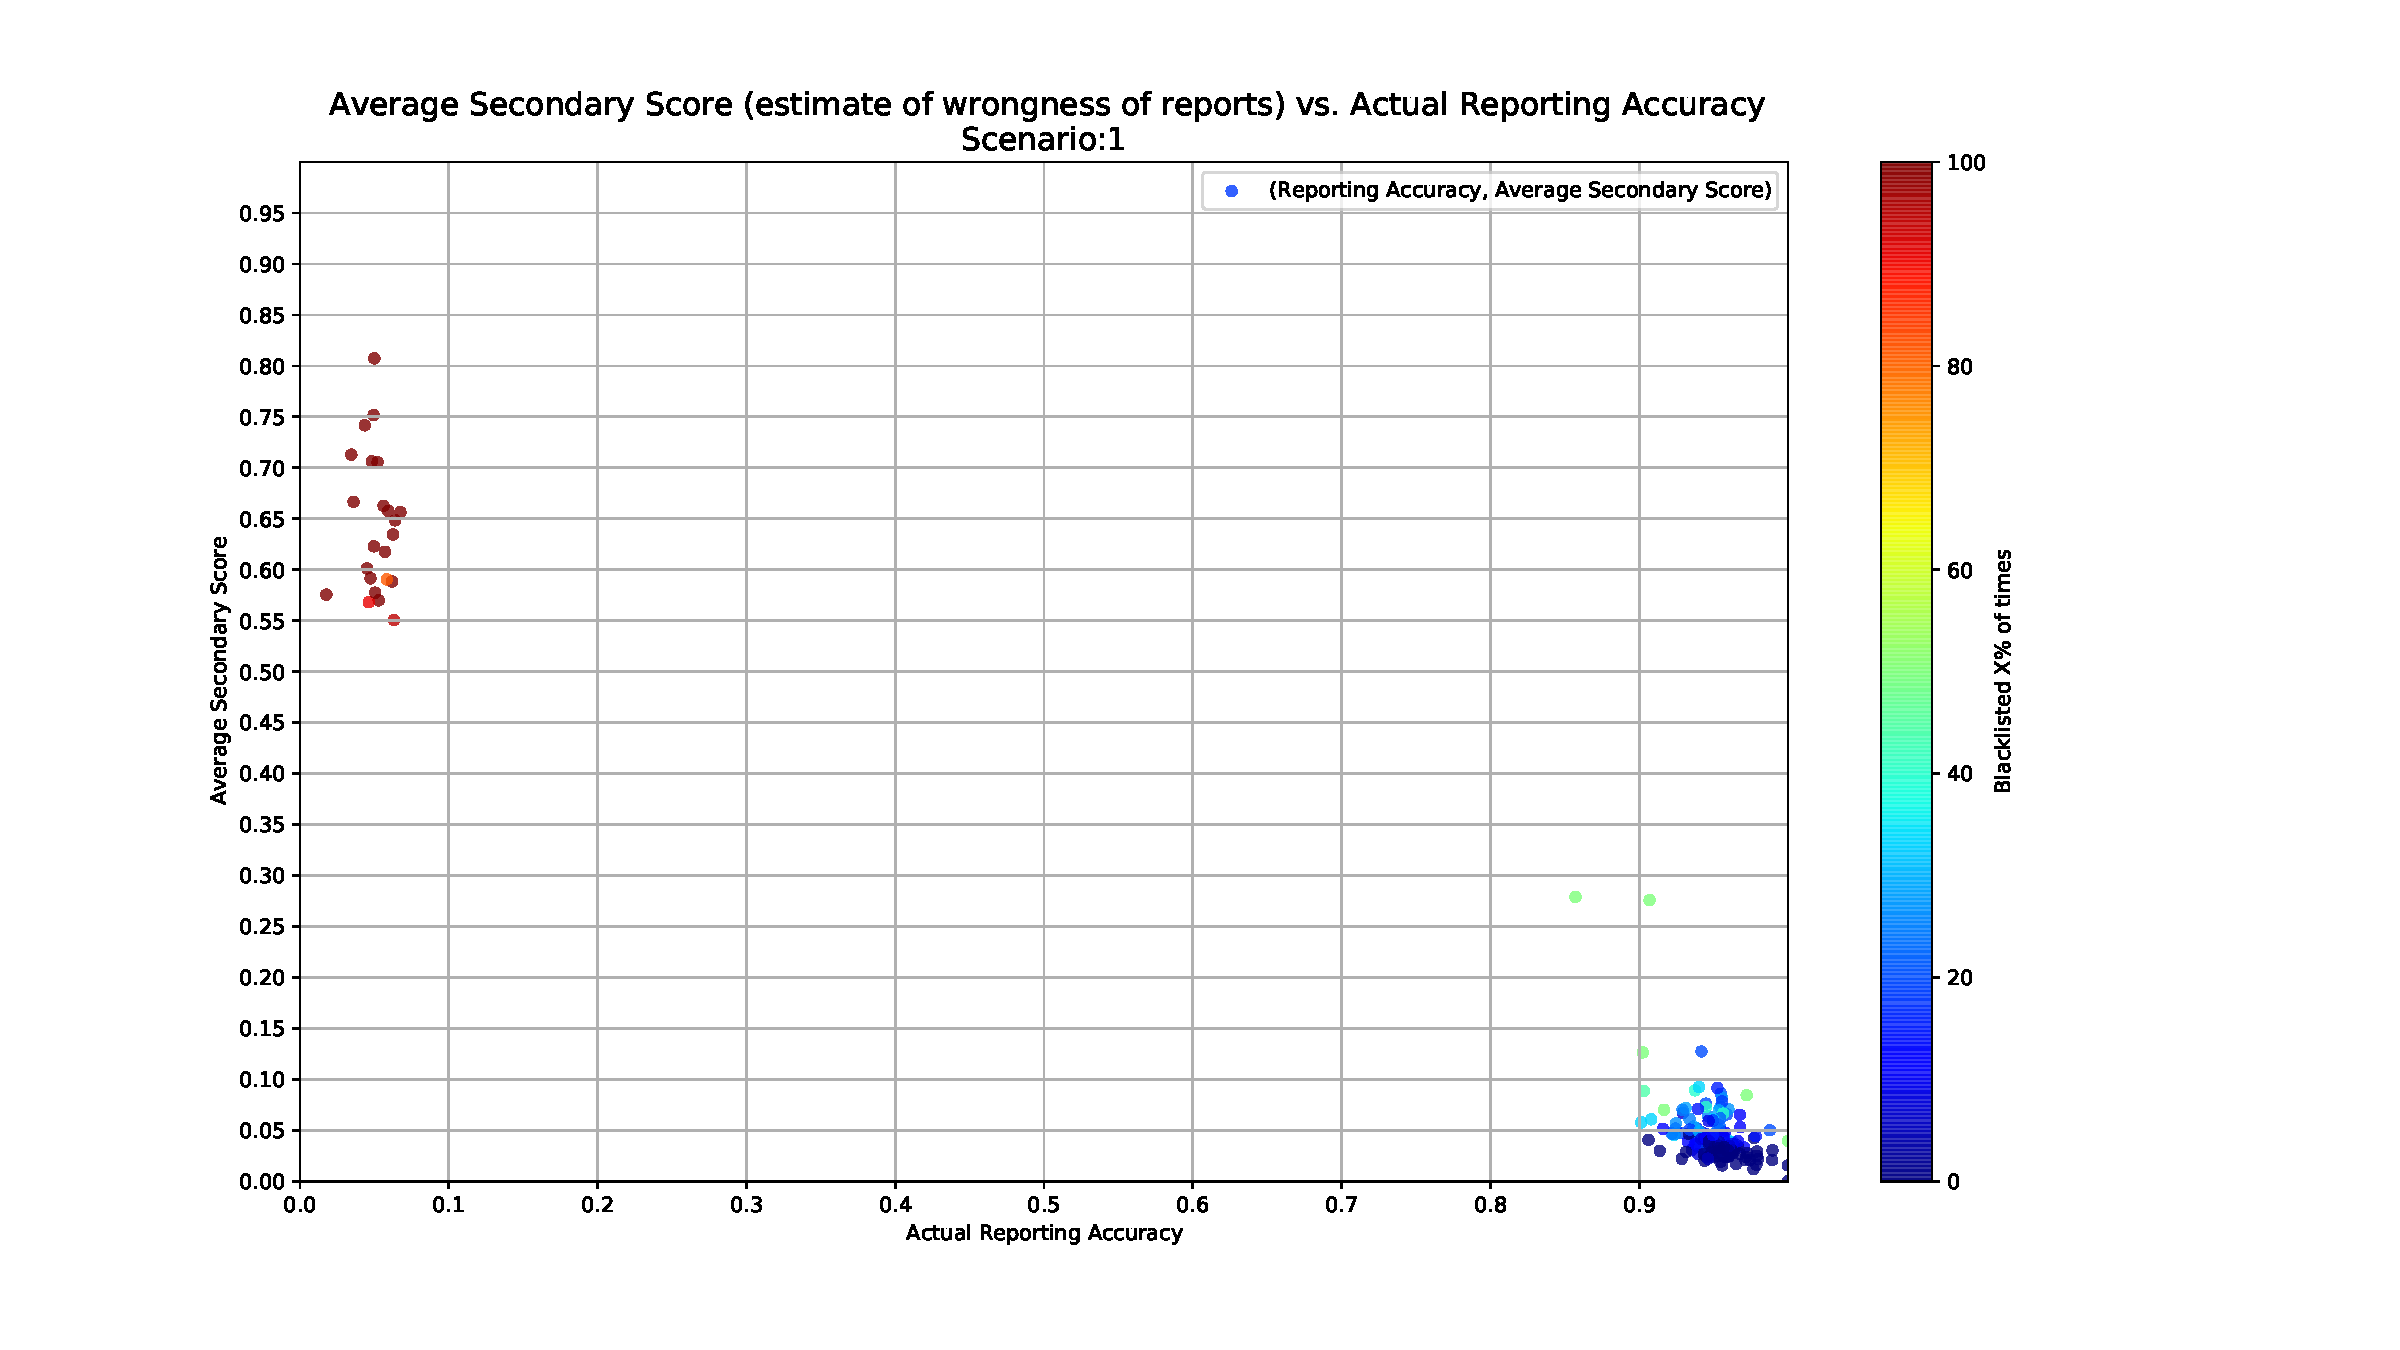
\includegraphics[width=0.5\linewidth,trim={100 50 185 72}, clip]{images/SCN1_ReportingAccuracy_Vs_AvgSecondaryScore.pdf}
	}
\end{figure*}
\begin{figure*}[!ht]
	\caption{Graphs for Results of Scenario 2). (a) Primary Score vs. Actual Accuracy - Scatter plot. (b) Primary Score and Actual Accuracy KDE. An Indicator of closeness of estimates. (c) Absolute error (difference between actual accuracy of node and estimated accuracy) vs. Percentage of nodes for which there was less than 'x'\% error. (d) Mean Secondary Score vs. Accuracy of Reports Sent - Scatter plot.}
	\label{fig:apdx:sc2}
	\centering
	\subfloat[]{
		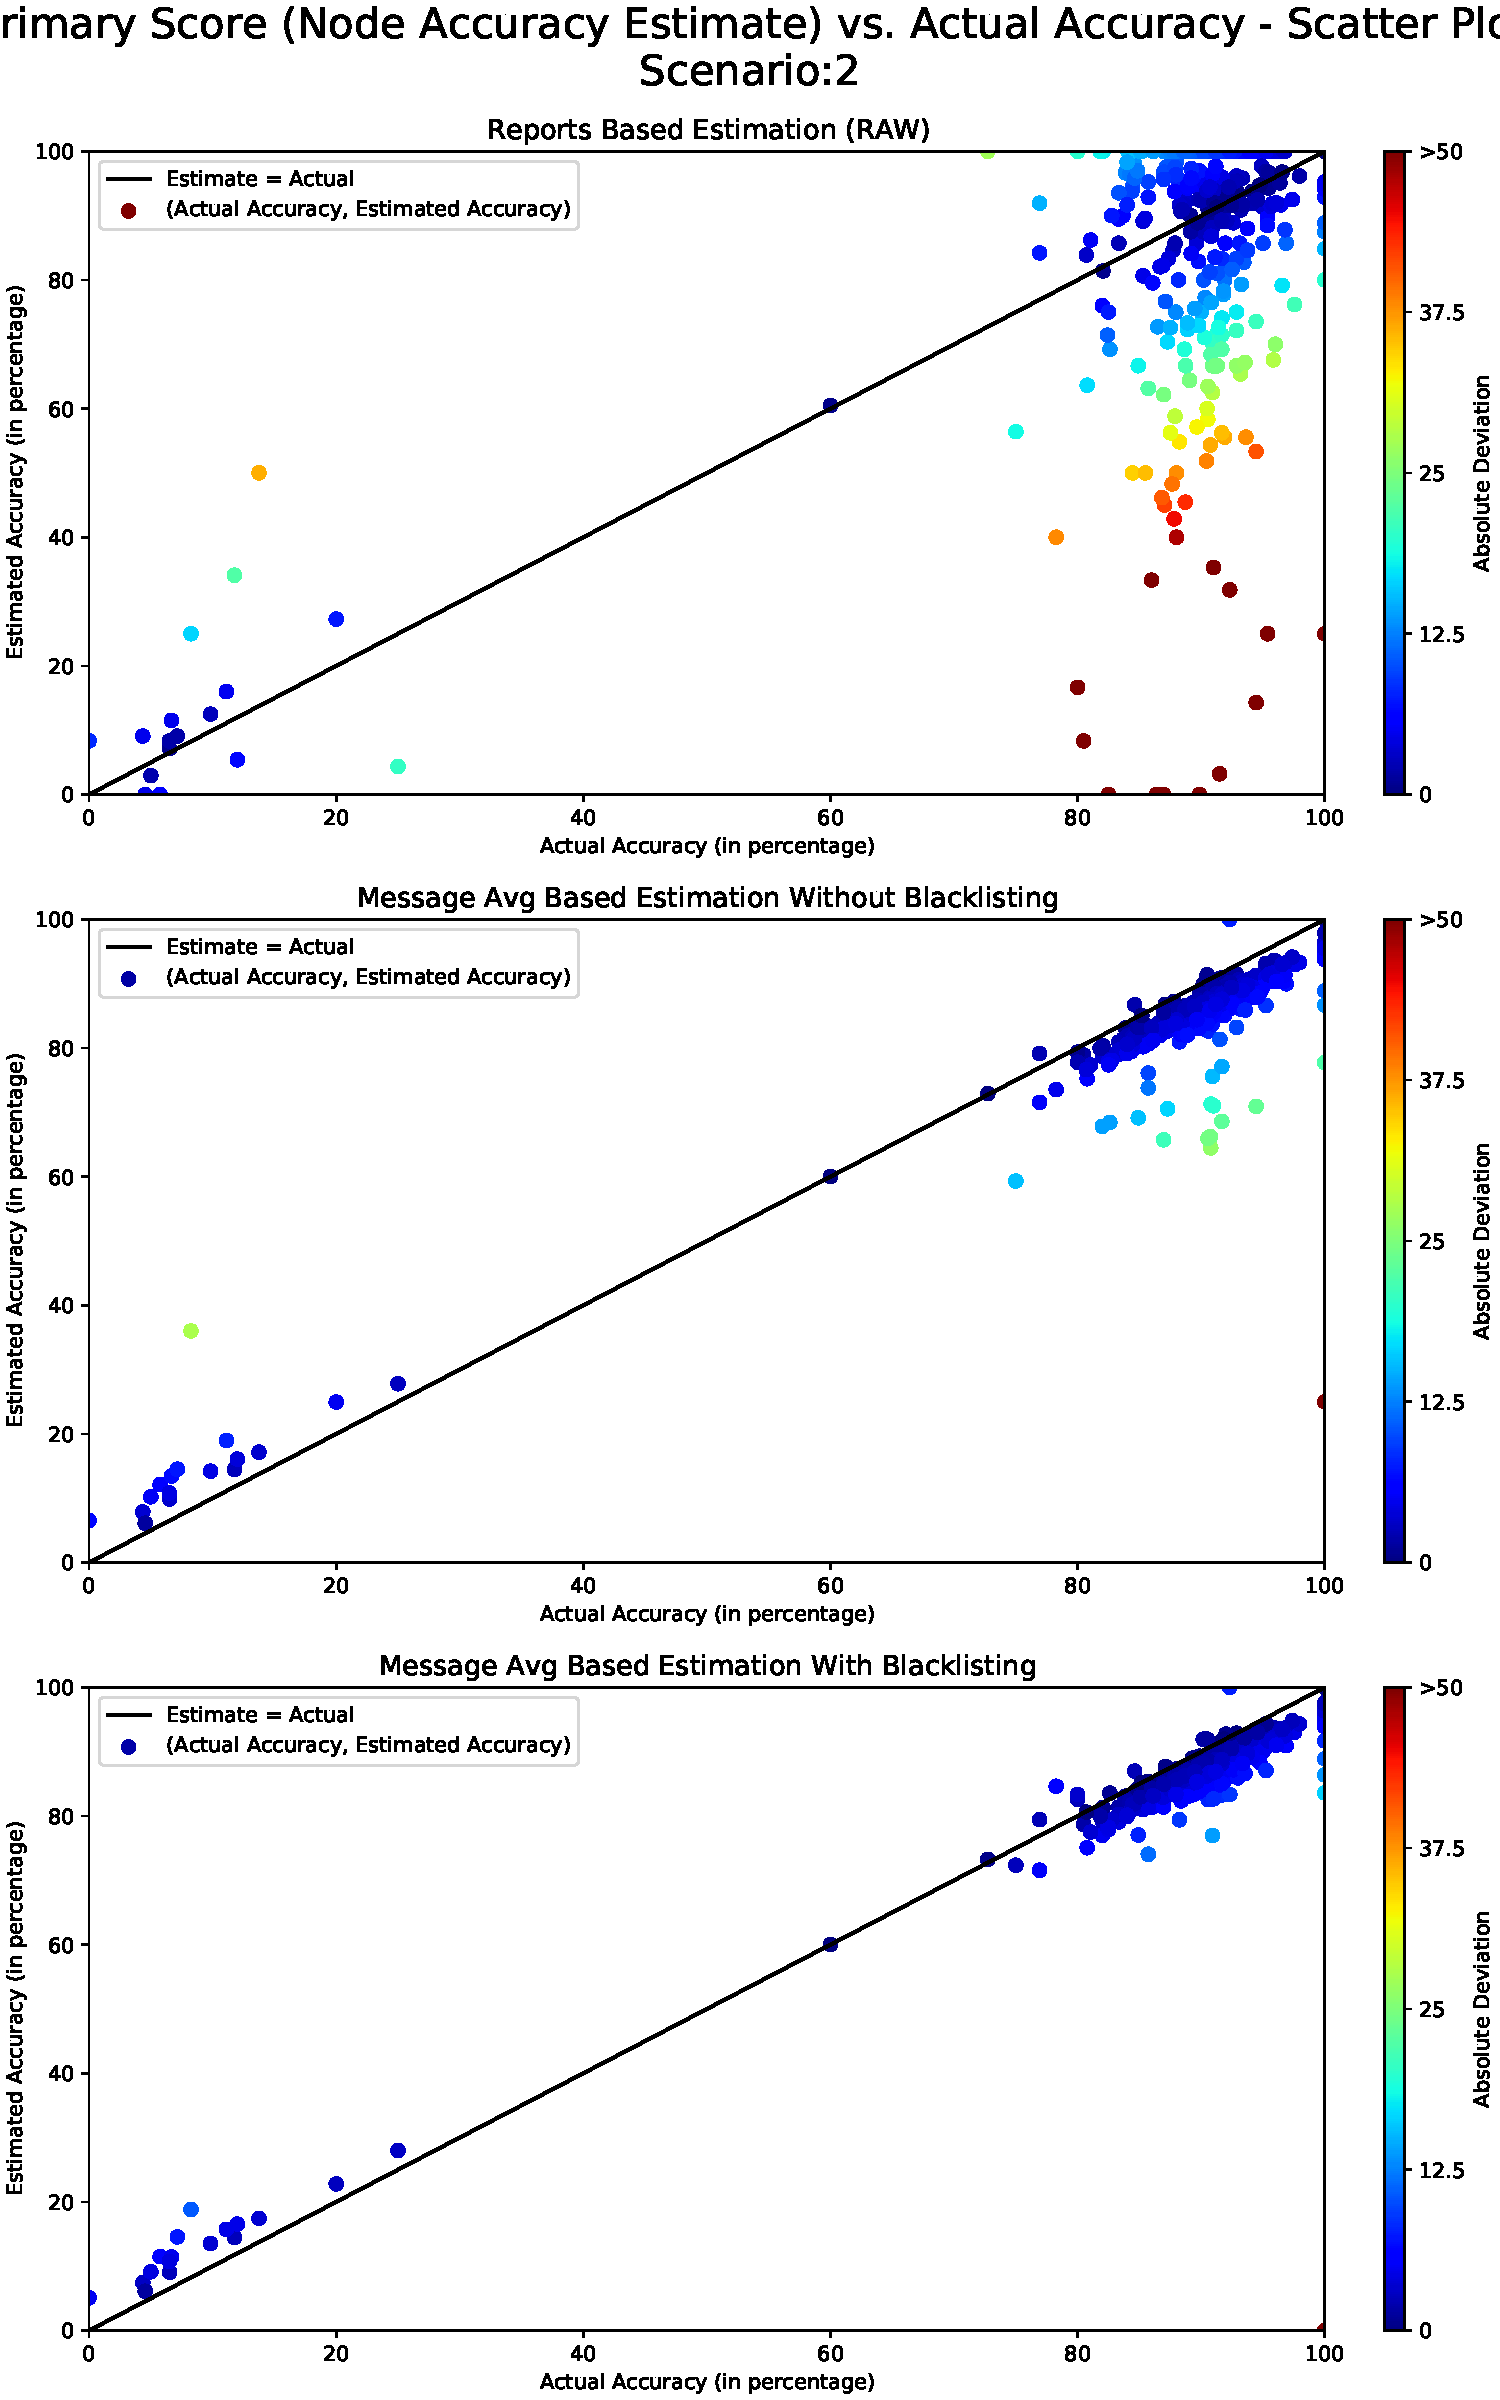
\includegraphics[width=0.5\linewidth, trim={0 5 15 50}, clip]{images/SCN2_PrimaryScoreVsActualAccuracyComparitive.pdf}
	}
	\subfloat[]{
		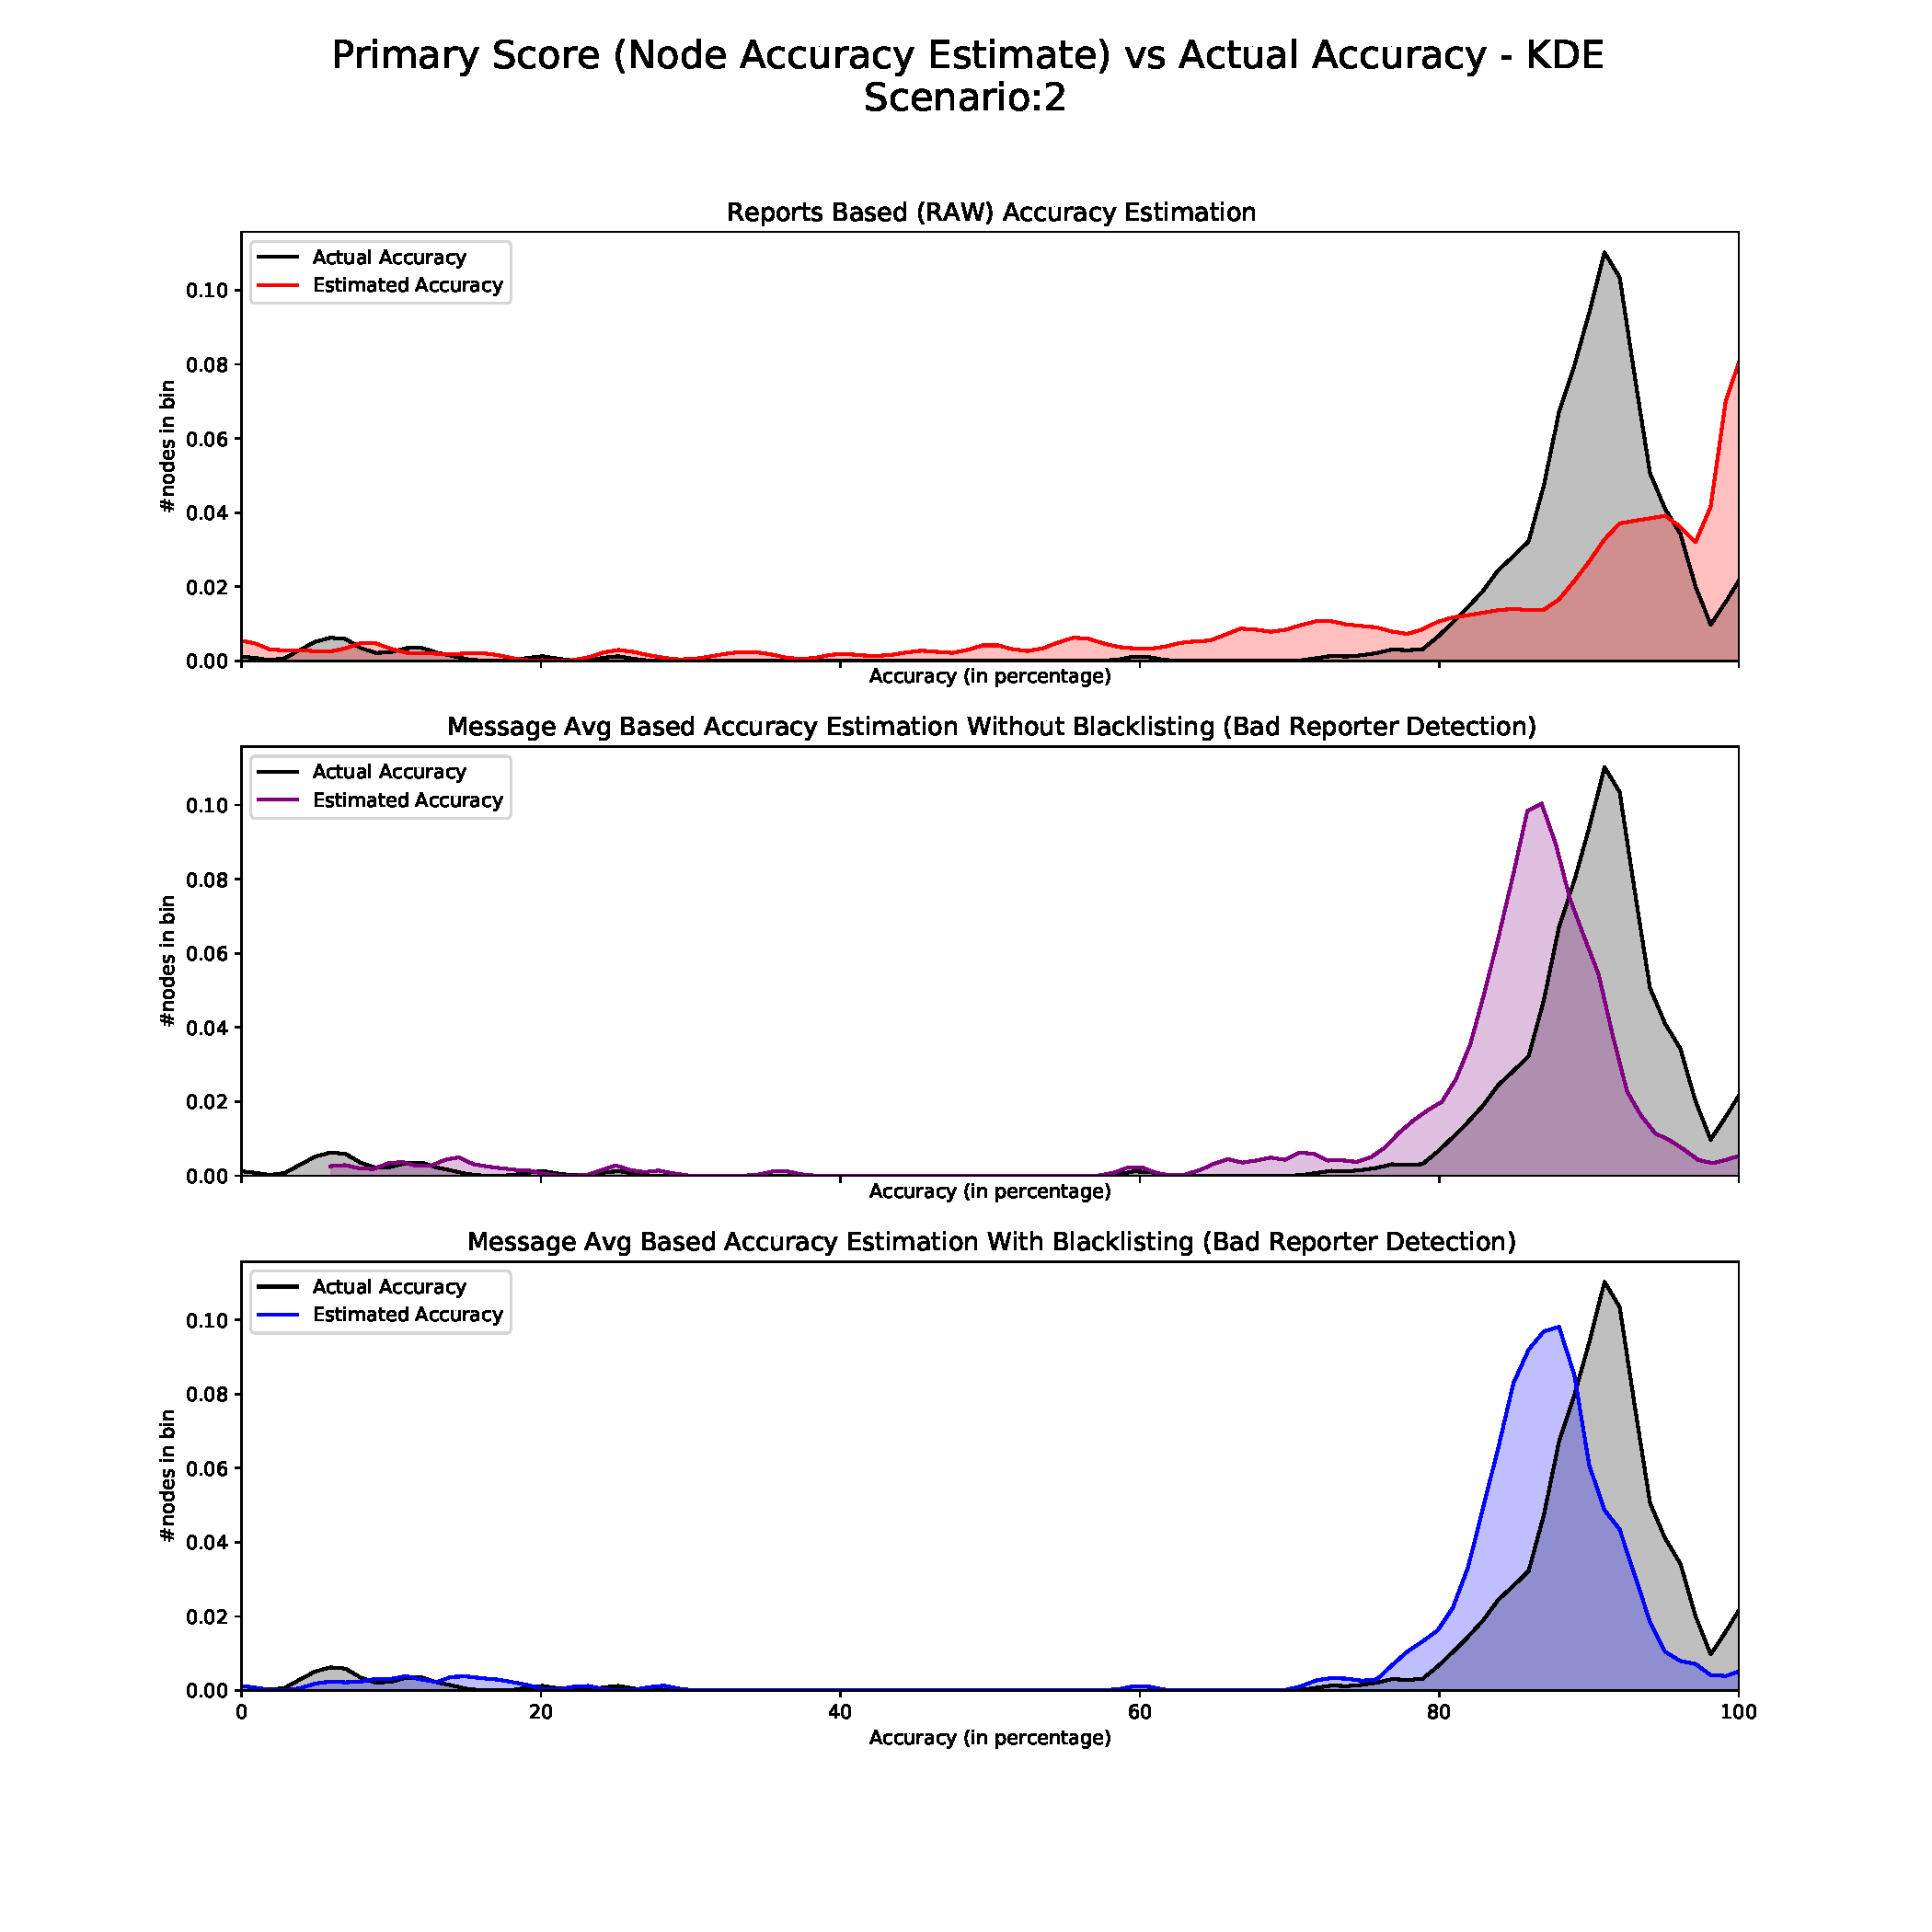
\includegraphics[width=0.5\linewidth, trim={80 95 100 100}, clip]{images/SCN2_PrimaryScoreKDEComparitive.pdf}
	}
	\hfill
	\subfloat[]{
		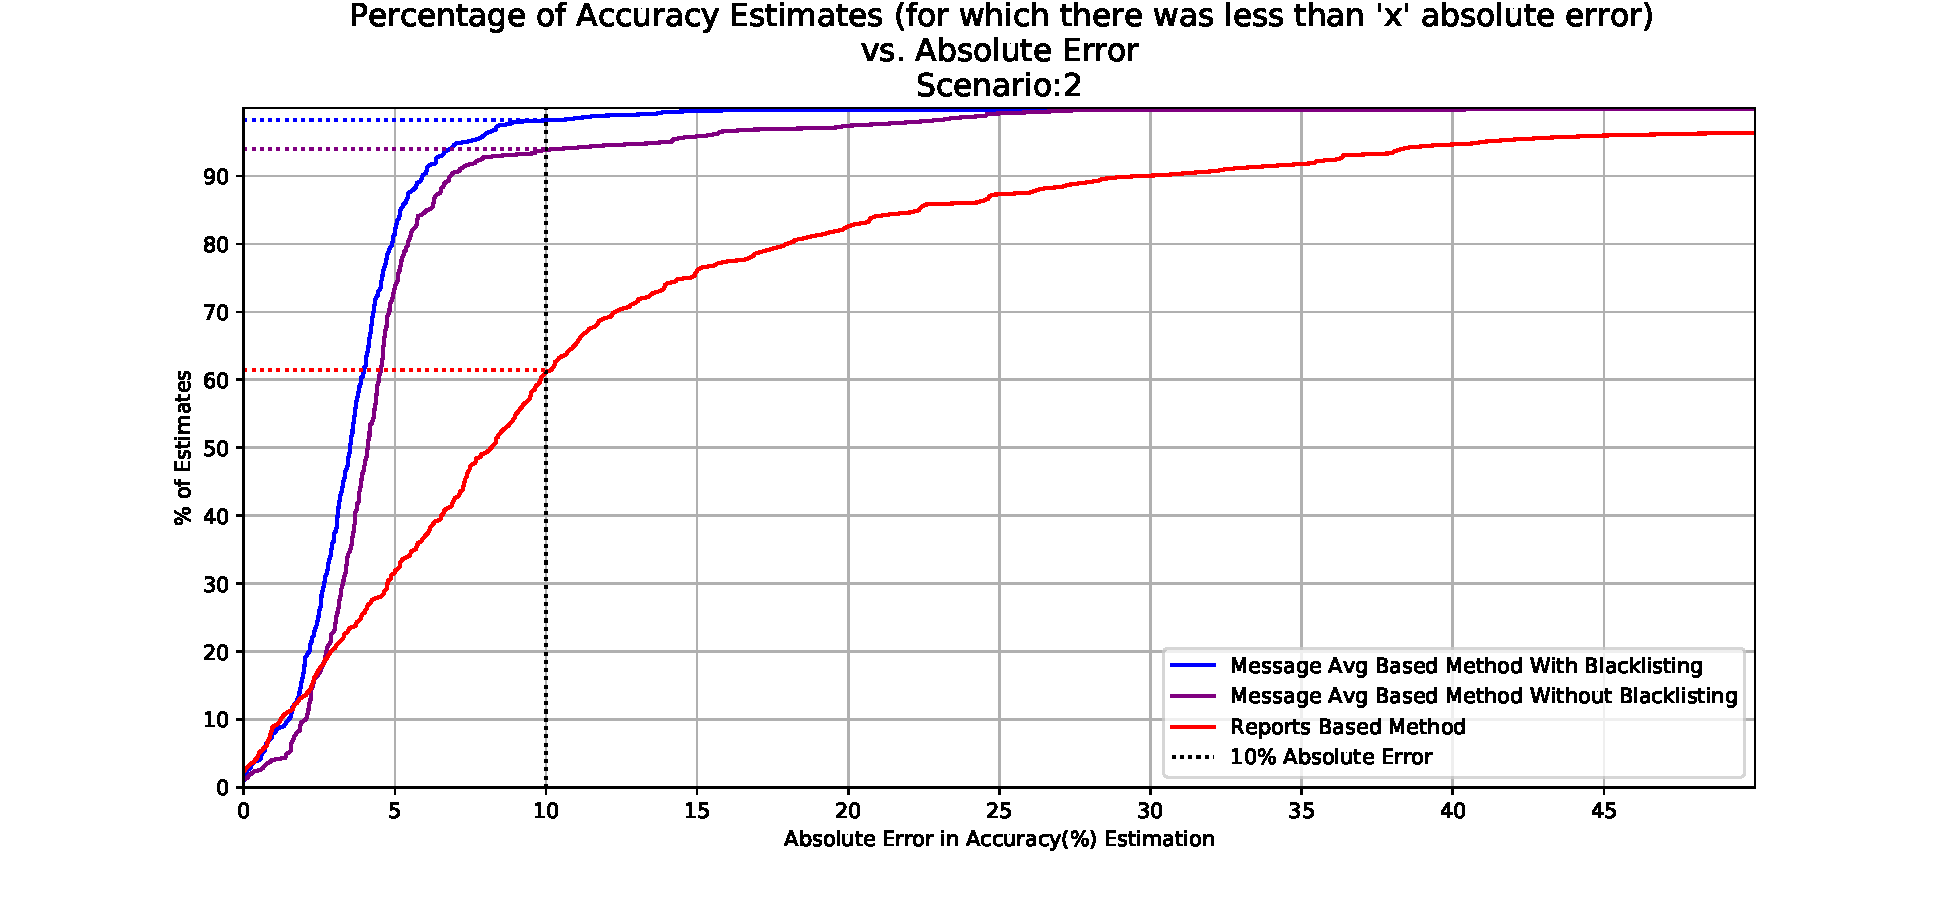
\includegraphics[width=0.5\linewidth, trim={80 25 90 50}, clip]{images/SCN2_AbsoluteErrorsInEstimationComparison.pdf}
	}
	\subfloat[]{
		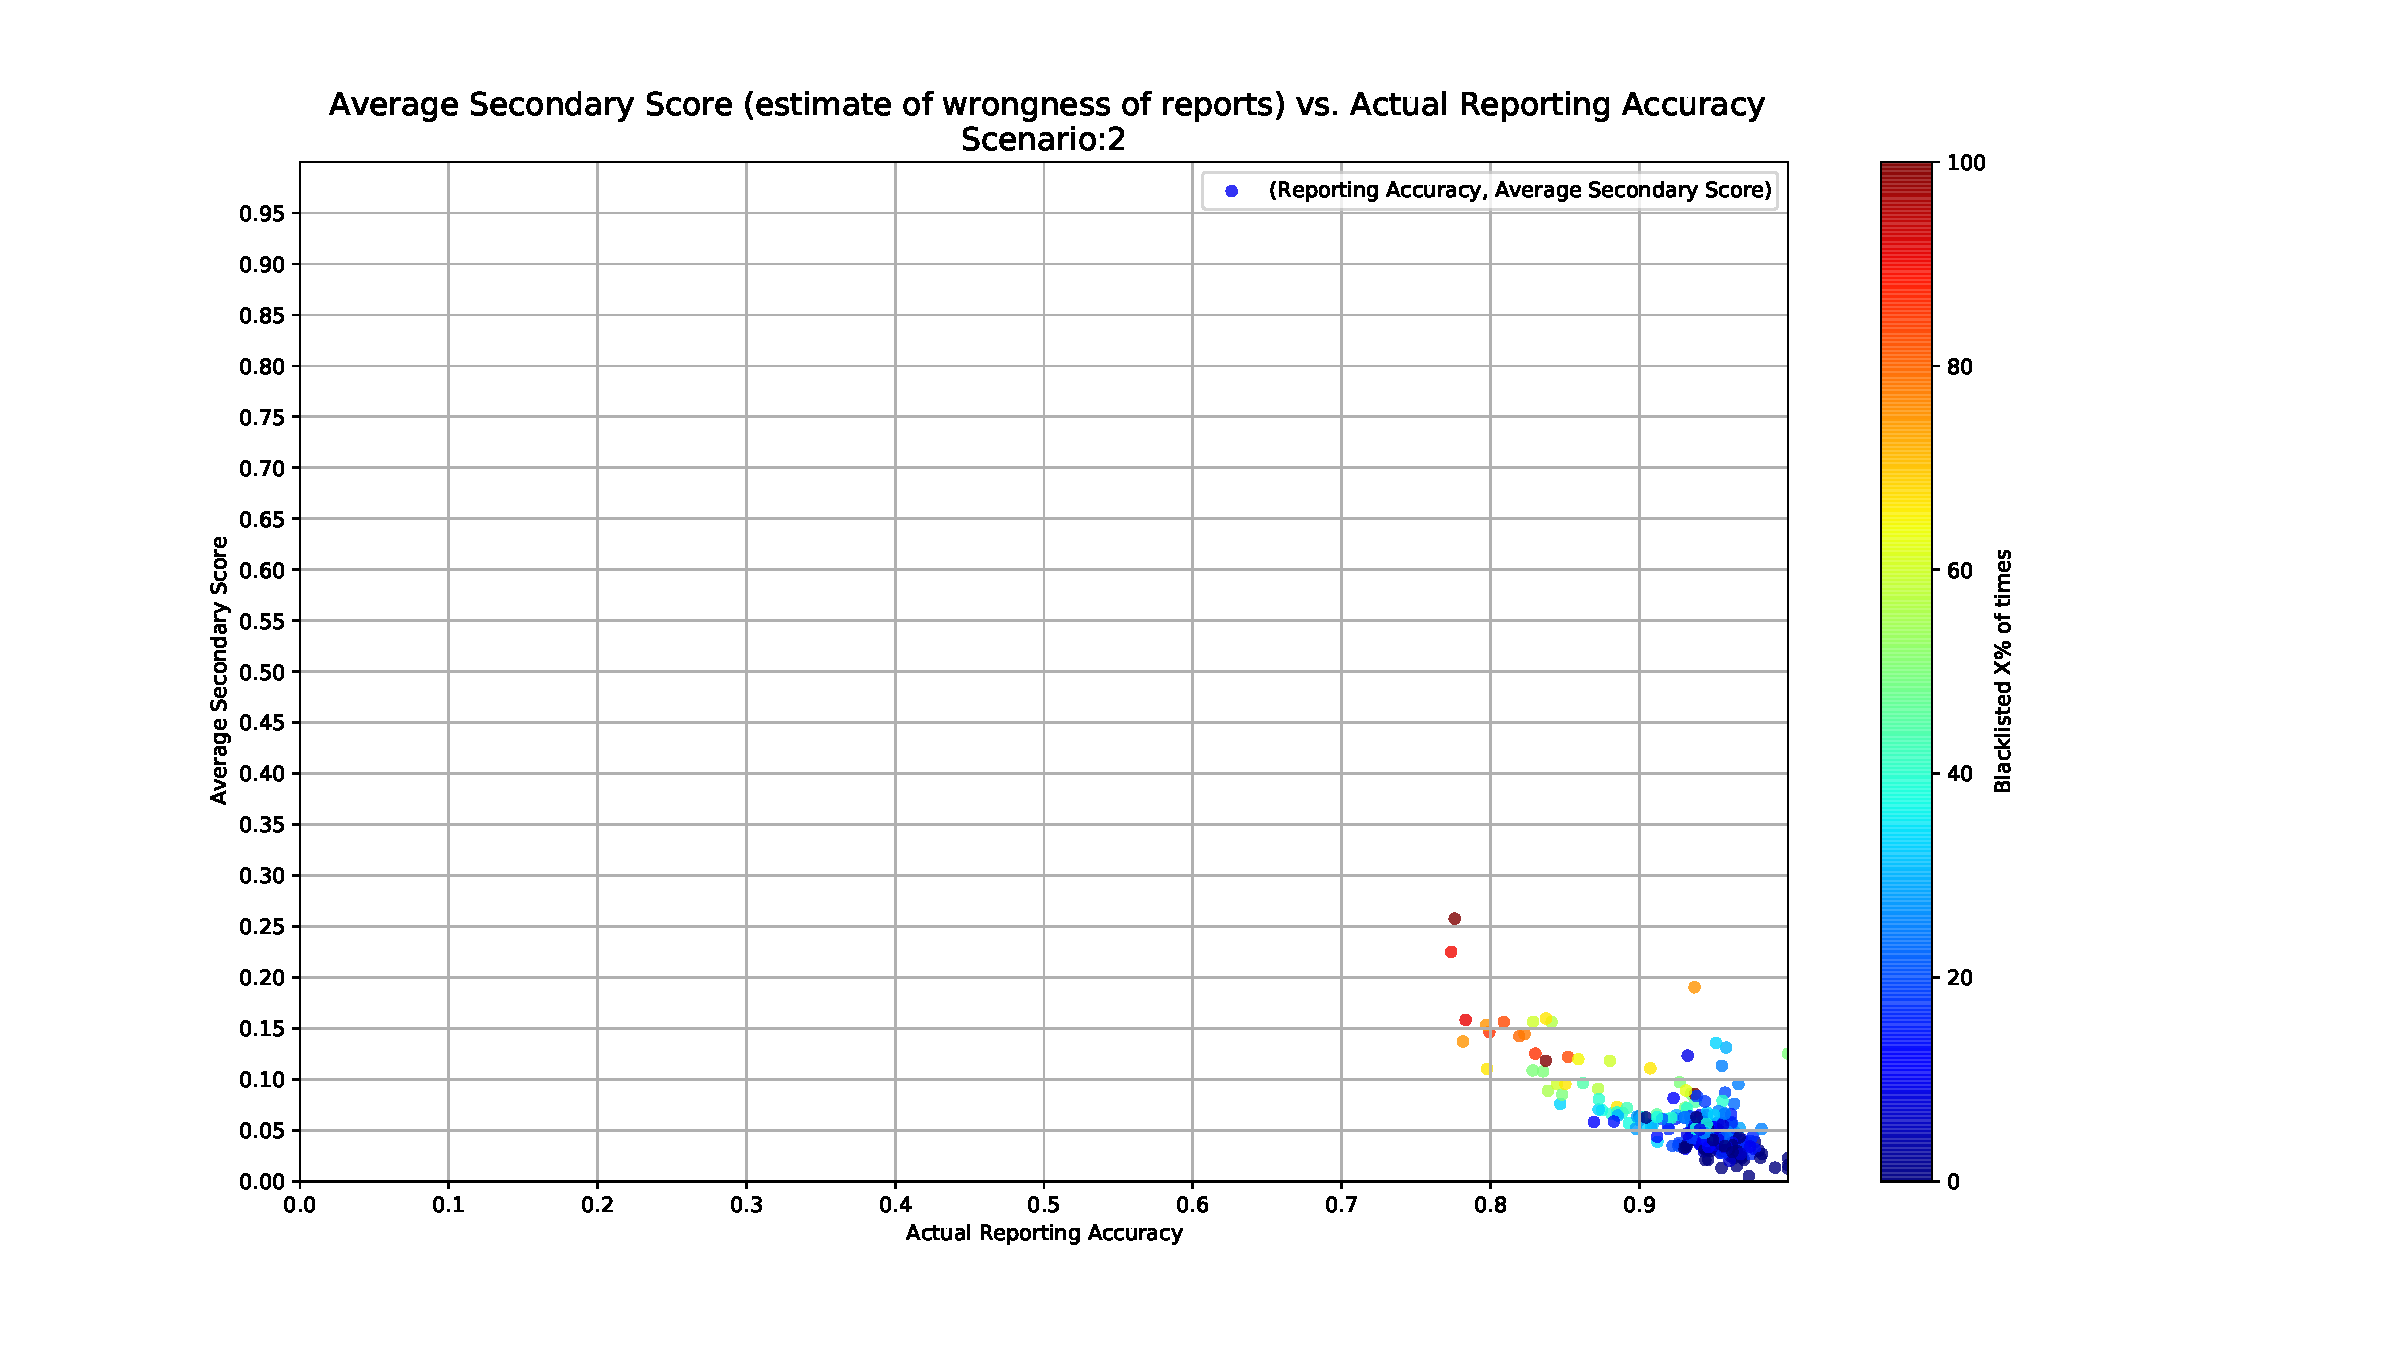
\includegraphics[width=0.5\linewidth,trim={100 50 185 72}, clip]{images/SCN2_ReportingAccuracy_Vs_AvgSecondaryScore.pdf}
	}
\end{figure*}
\begin{figure*}[!ht]
	\caption{Graphs for Results of Scenario 10. (a) Primary Score vs. Actual Accuracy - Scatter plot. (b) Primary Score and Actual Accuracy KDE. An Indicator of closeness of estimates. (c) Absolute error (difference between actual accuracy of node and estimated accuracy) vs. Percentage of nodes for which there was less than 'x'\% error. (d) Mean Secondary Score vs. Accuracy of Reports Sent - Scatter plot.}
	\label{fig:apdx:sc10}
	\centering
	\subfloat[]{
		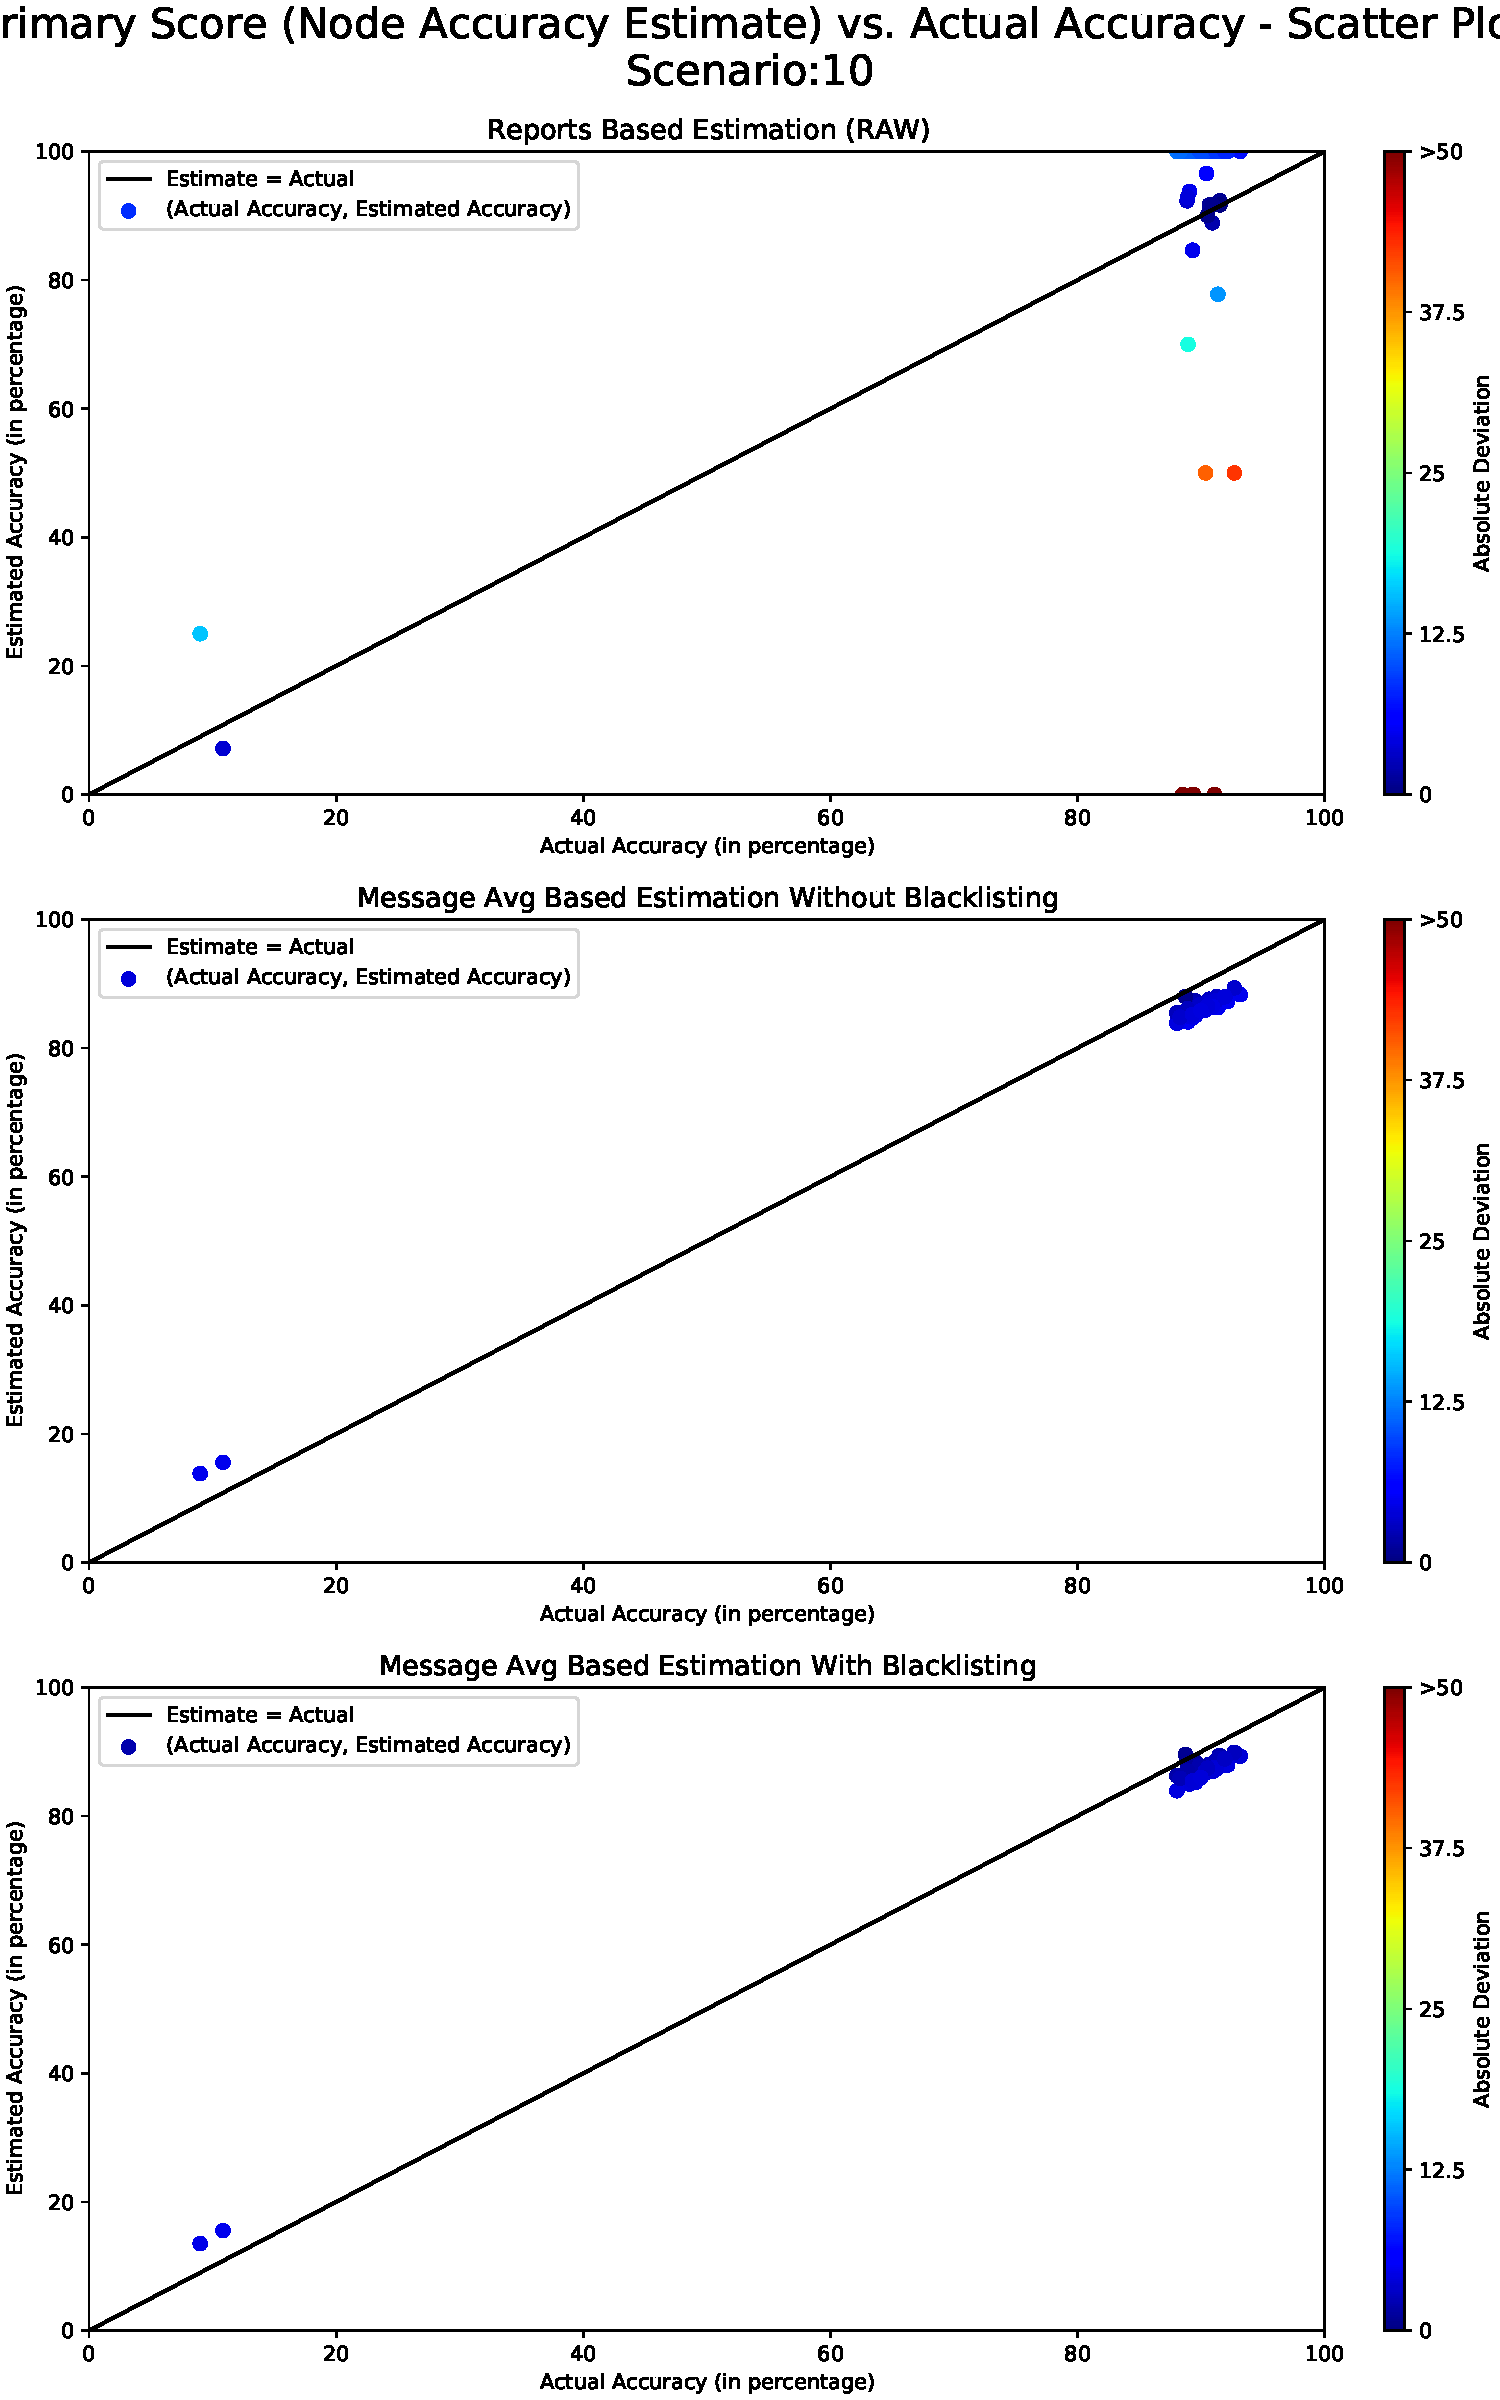
\includegraphics[width=0.5\linewidth, trim={0 5 15 50}, clip]{images/SCN10_PrimaryScoreVsActualAccuracyComparitive.pdf}
	}
	\subfloat[]{
		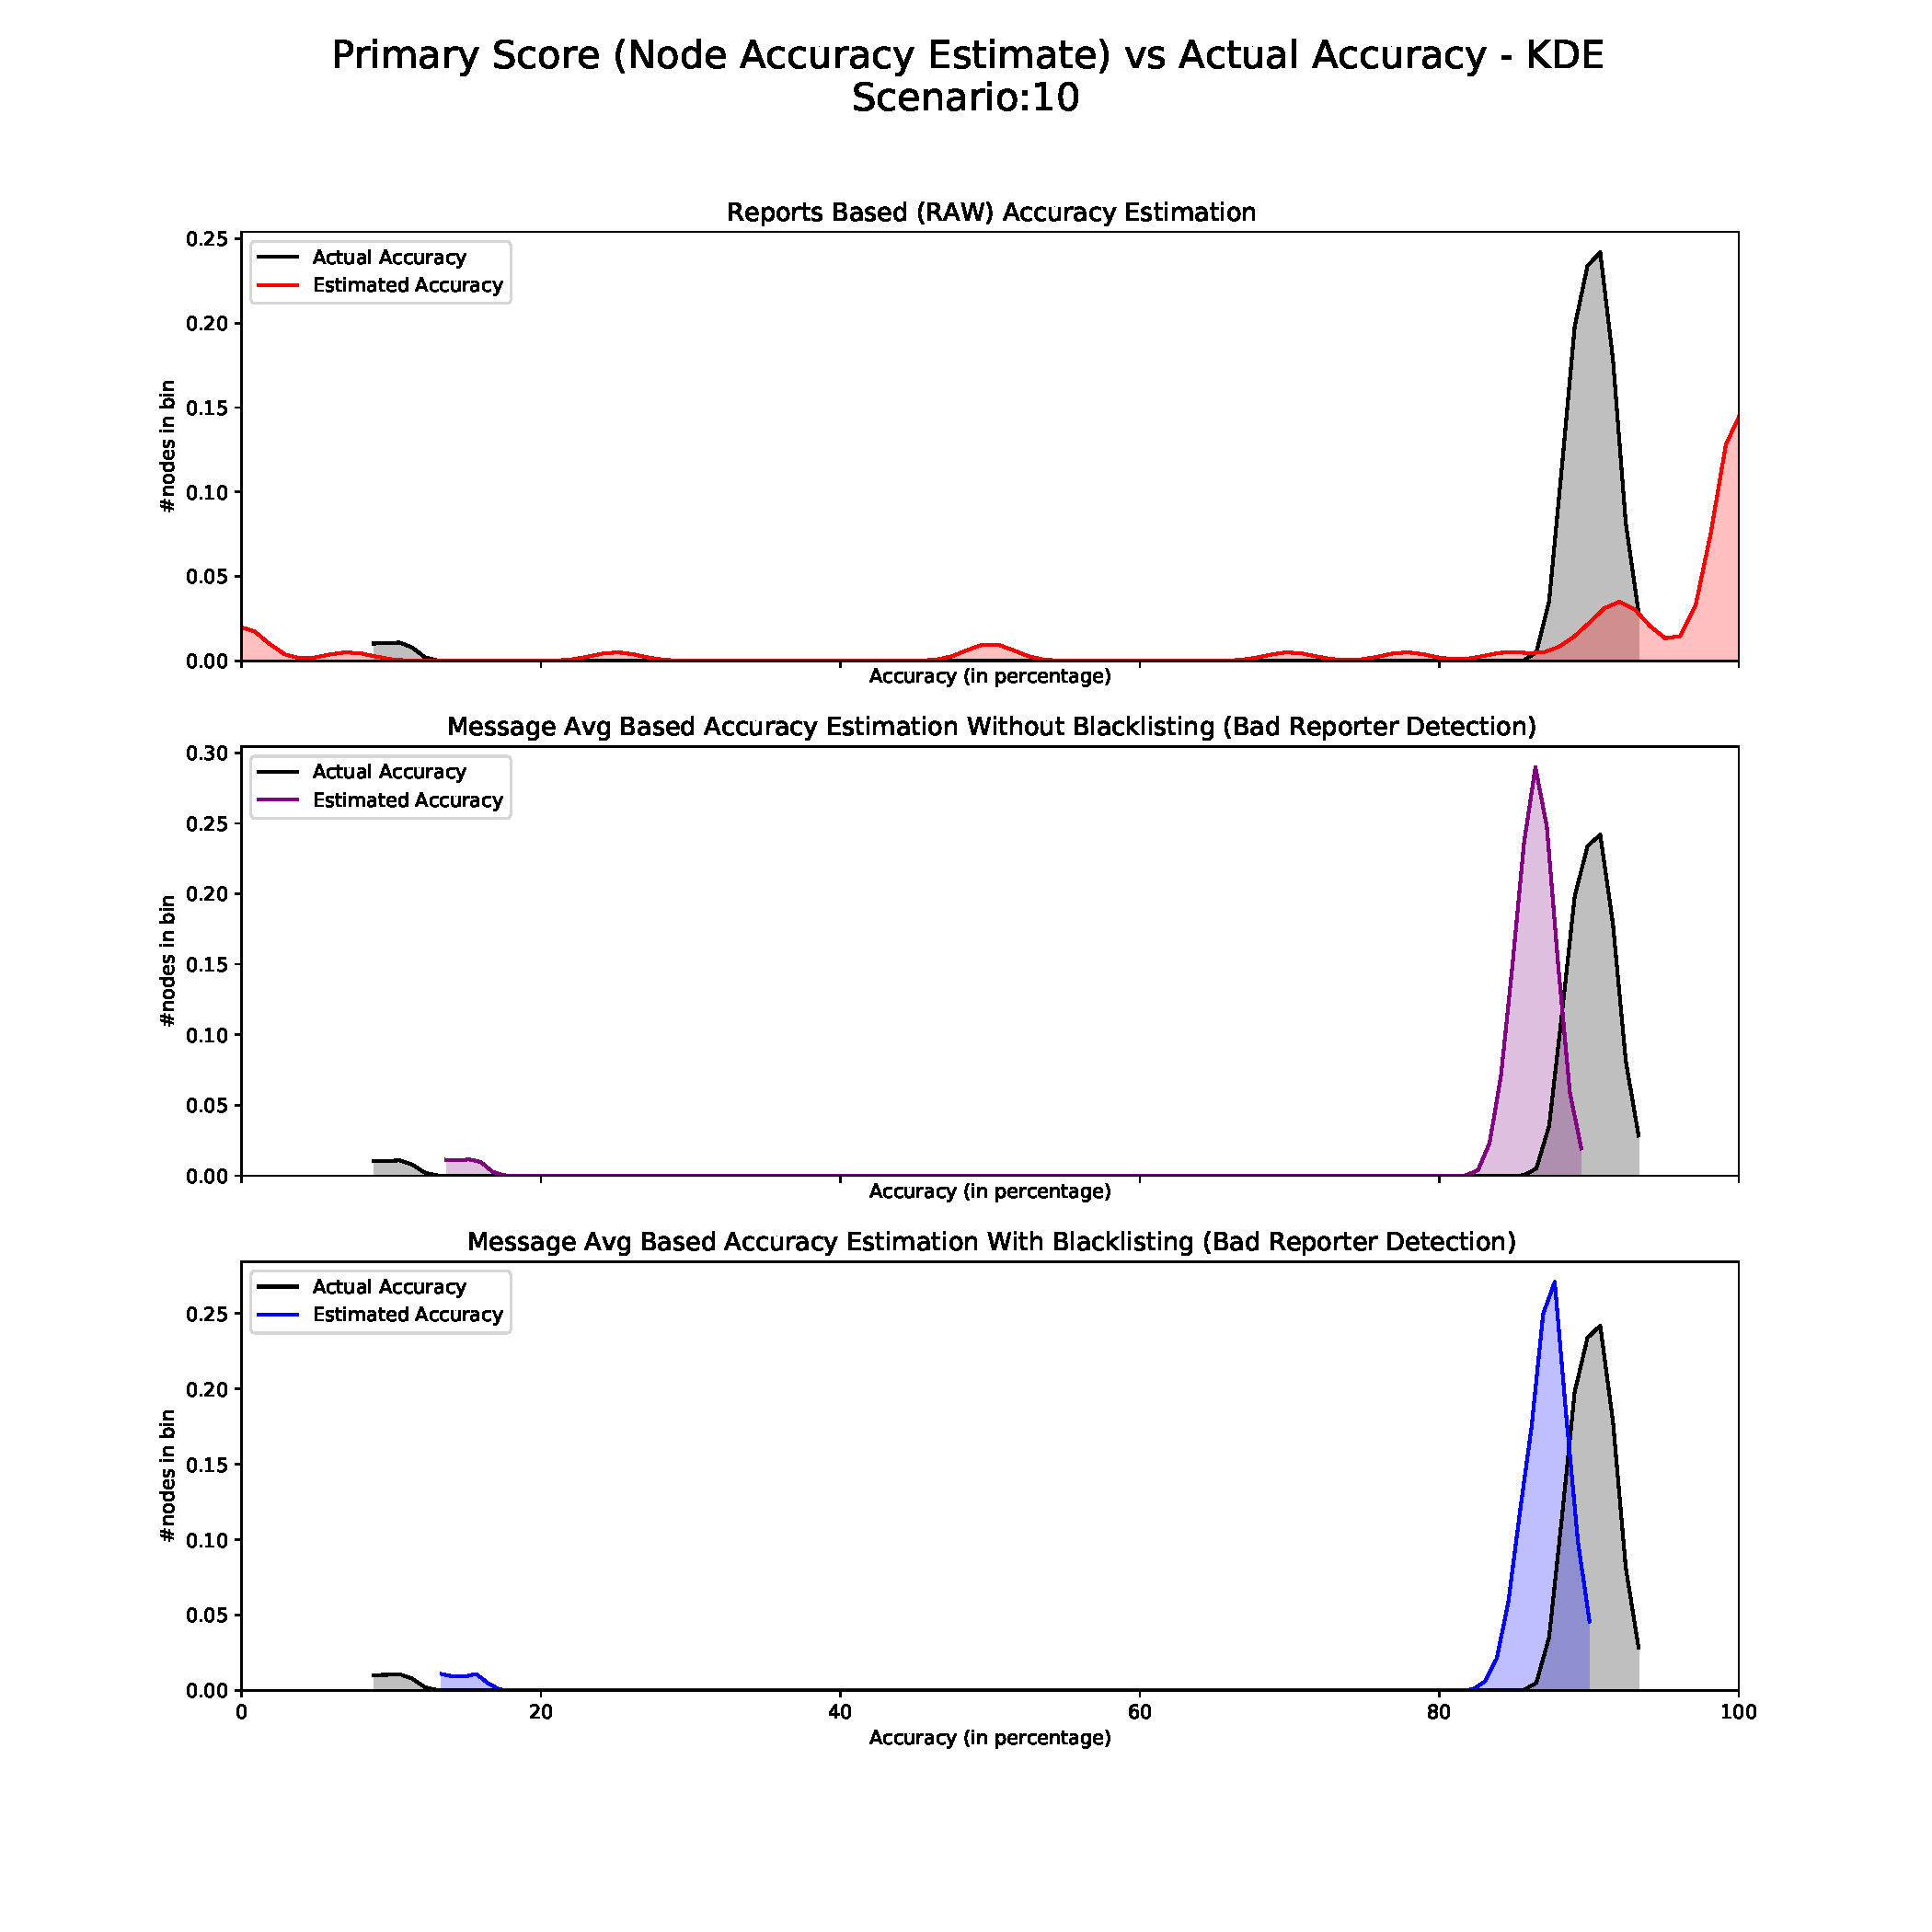
\includegraphics[width=0.5\linewidth, trim={80 95 100 100}, clip]{images/SCN10_PrimaryScoreKDEComparitive.pdf}
	}
	\hfill
	\subfloat[]{
		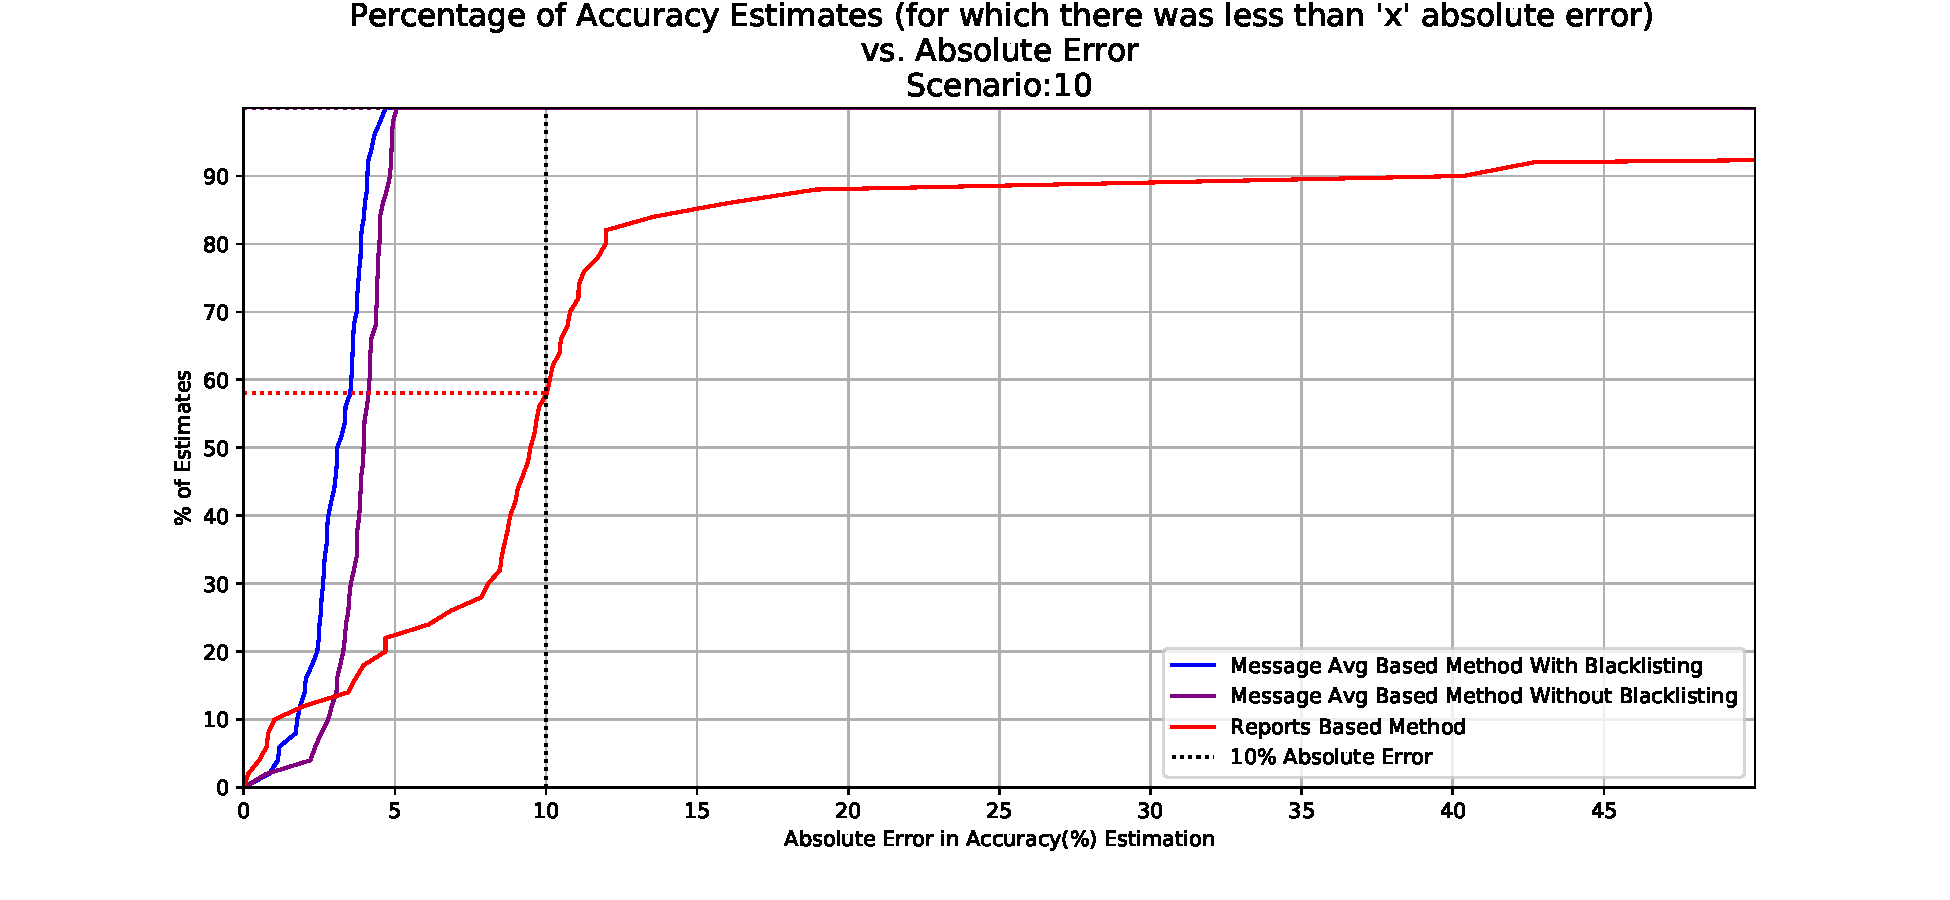
\includegraphics[width=0.5\linewidth, trim={80 25 90 50}, clip]{images/SCN10_AbsoluteErrorsInEstimationComparison.pdf}
	}
	\subfloat[]{
		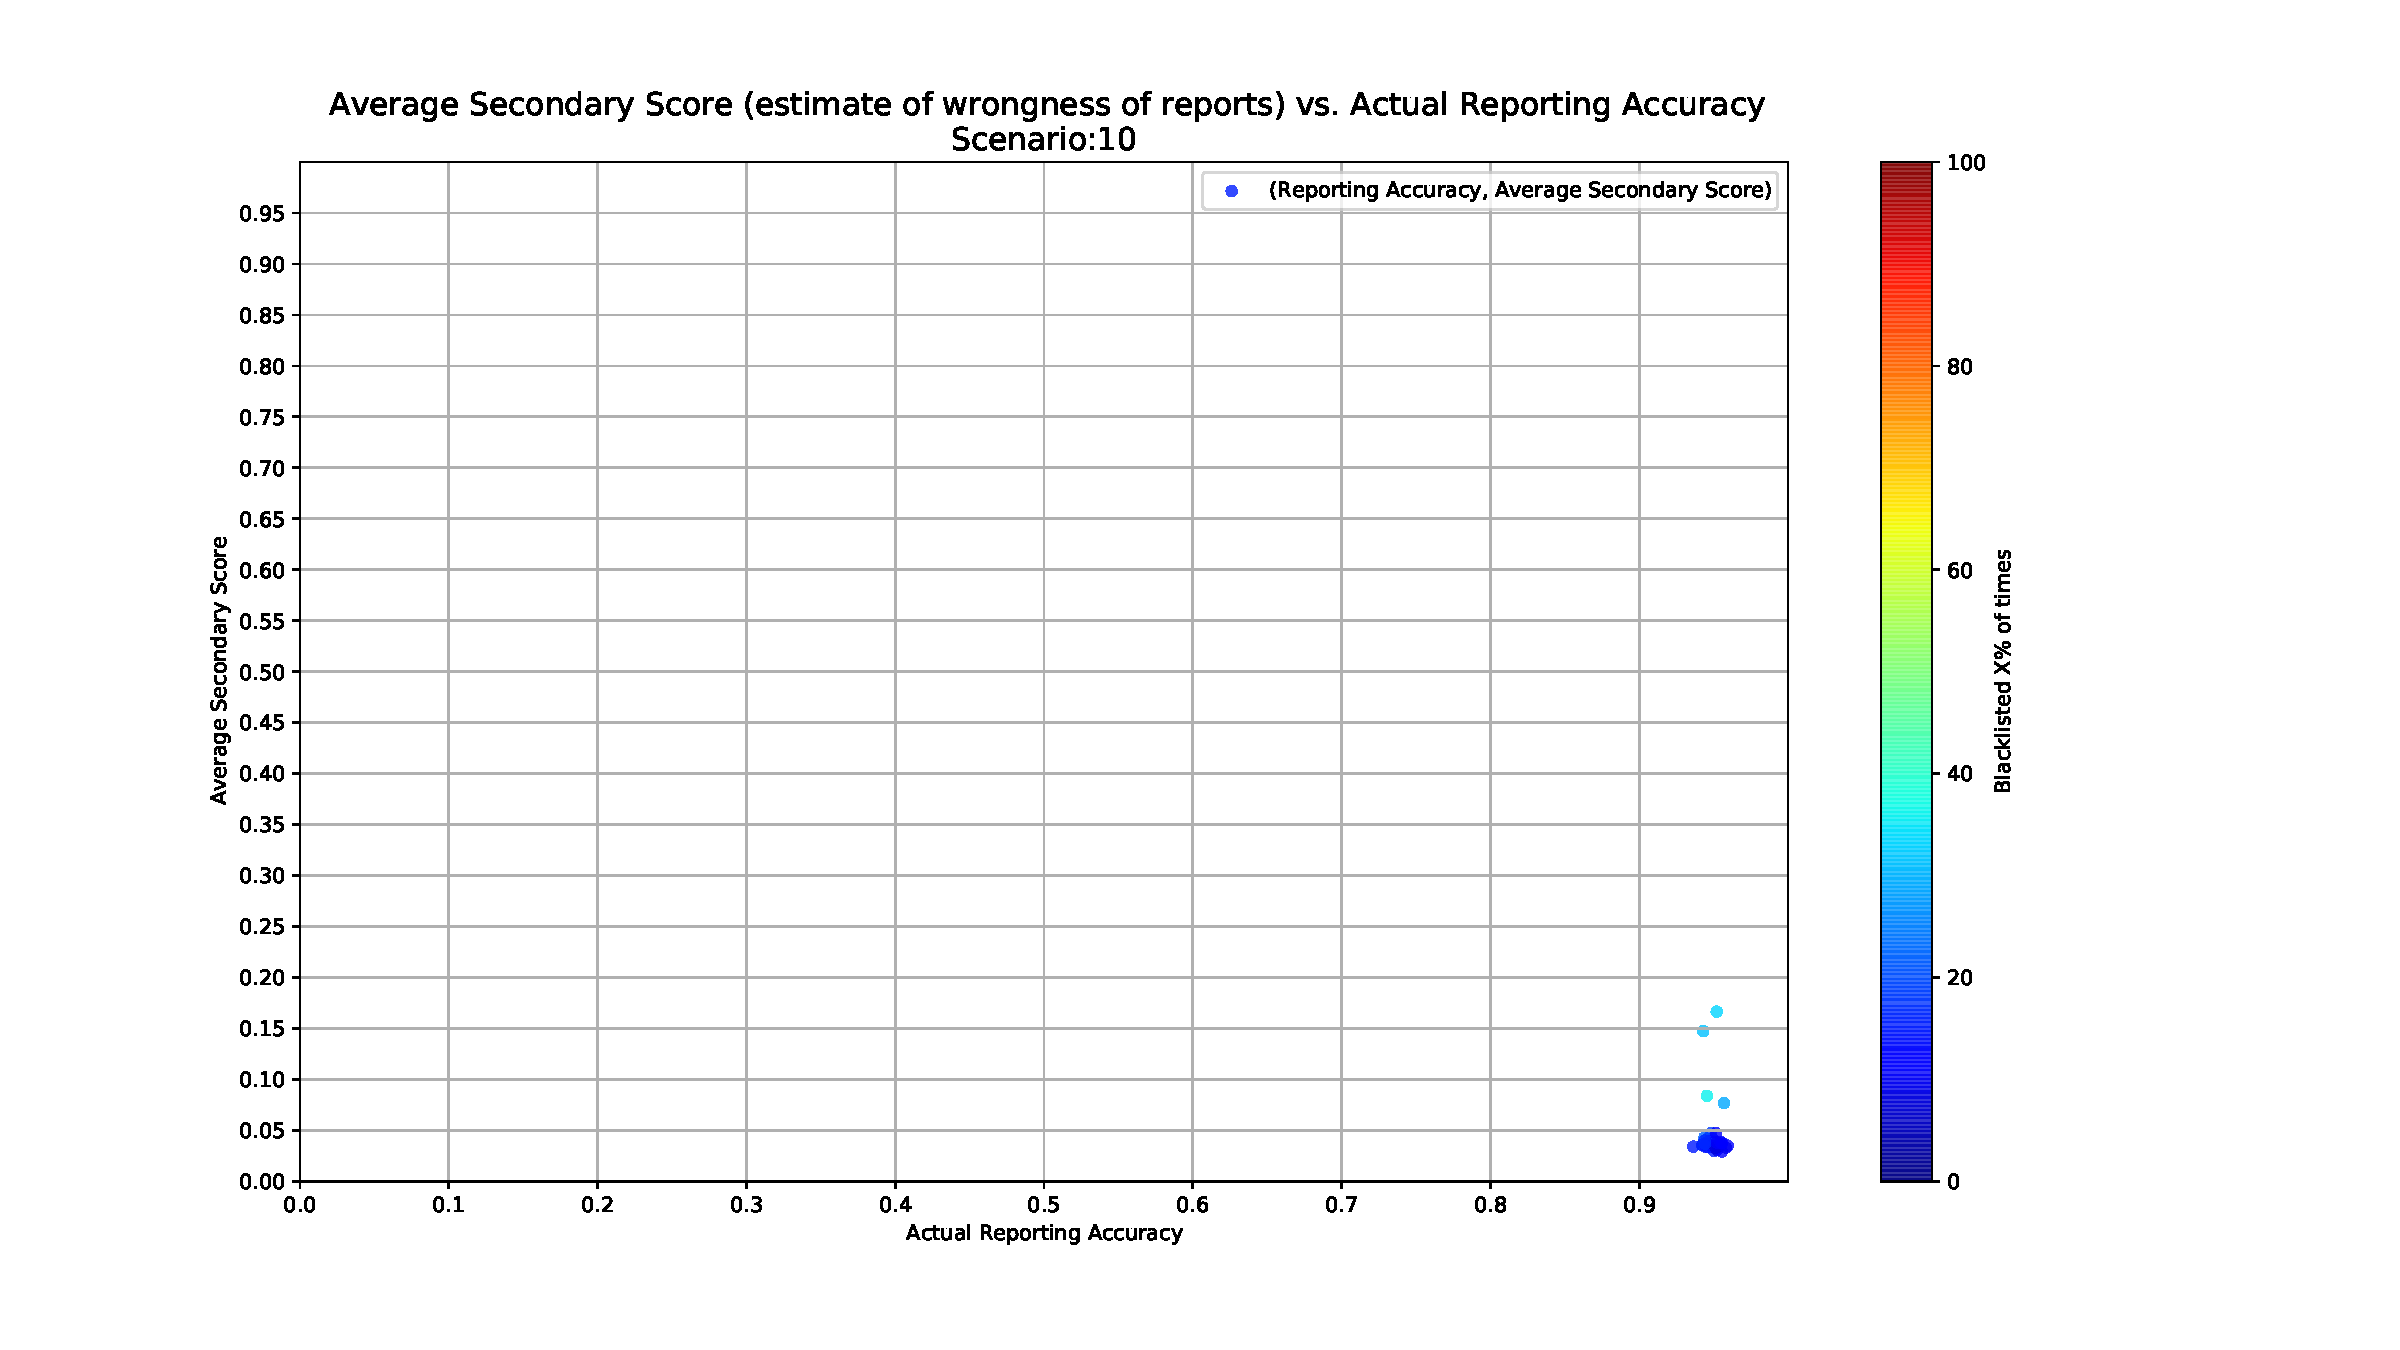
\includegraphics[width=0.5\linewidth,trim={100 50 185 72}, clip]{images/SCN10_ReportingAccuracy_Vs_AvgSecondaryScore.pdf}
	}
\end{figure*}
\begin{figure*}[!ht]
	\caption{Graphs for Results of Scenario 11. (a) Primary Score vs. Actual Accuracy - Scatter plot. (b) Primary Score and Actual Accuracy KDE. An Indicator of closeness of estimates. (c) Absolute error (difference between actual accuracy of node and estimated accuracy) vs. Percentage of nodes for which there was less than 'x'\% error. (d) Mean Secondary Score vs. Accuracy of Reports Sent - Scatter plot.}
	\label{fig:apdx:sc11}
	\centering
	\subfloat[]{
		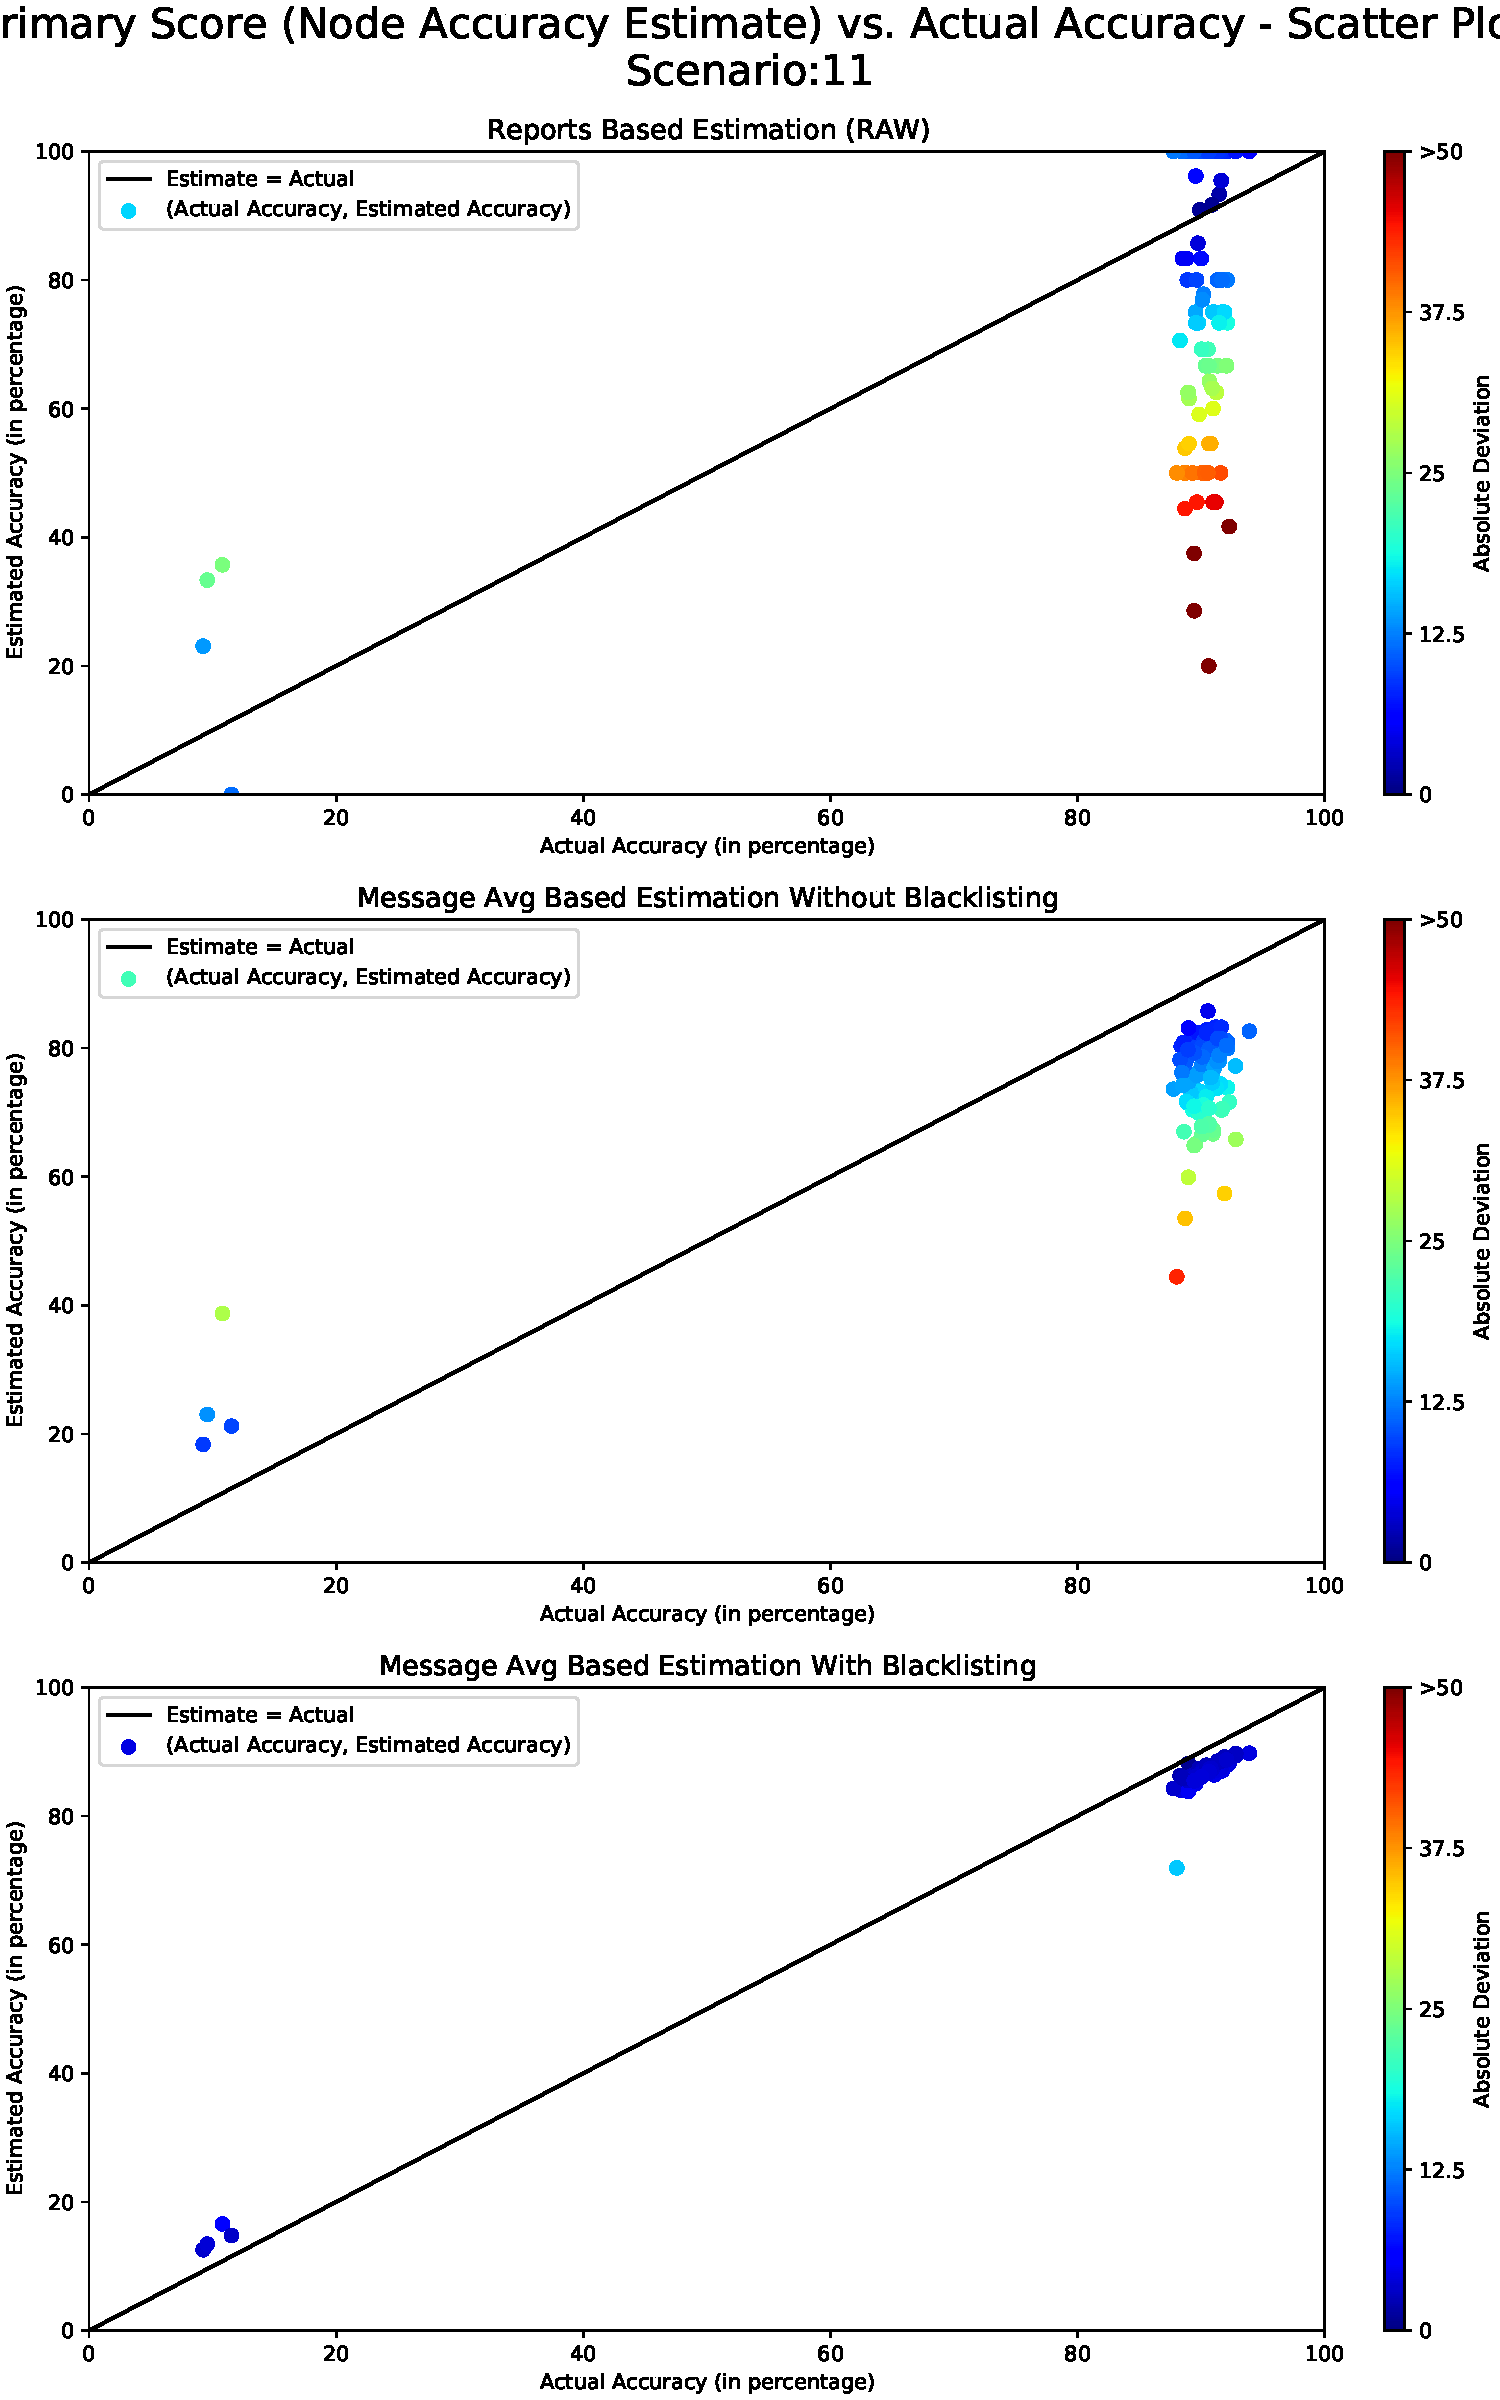
\includegraphics[width=0.5\linewidth, trim={0 5 15 50}, clip]{images/SCN11_PrimaryScoreVsActualAccuracyComparitive.pdf}
	}
	\subfloat[]{
		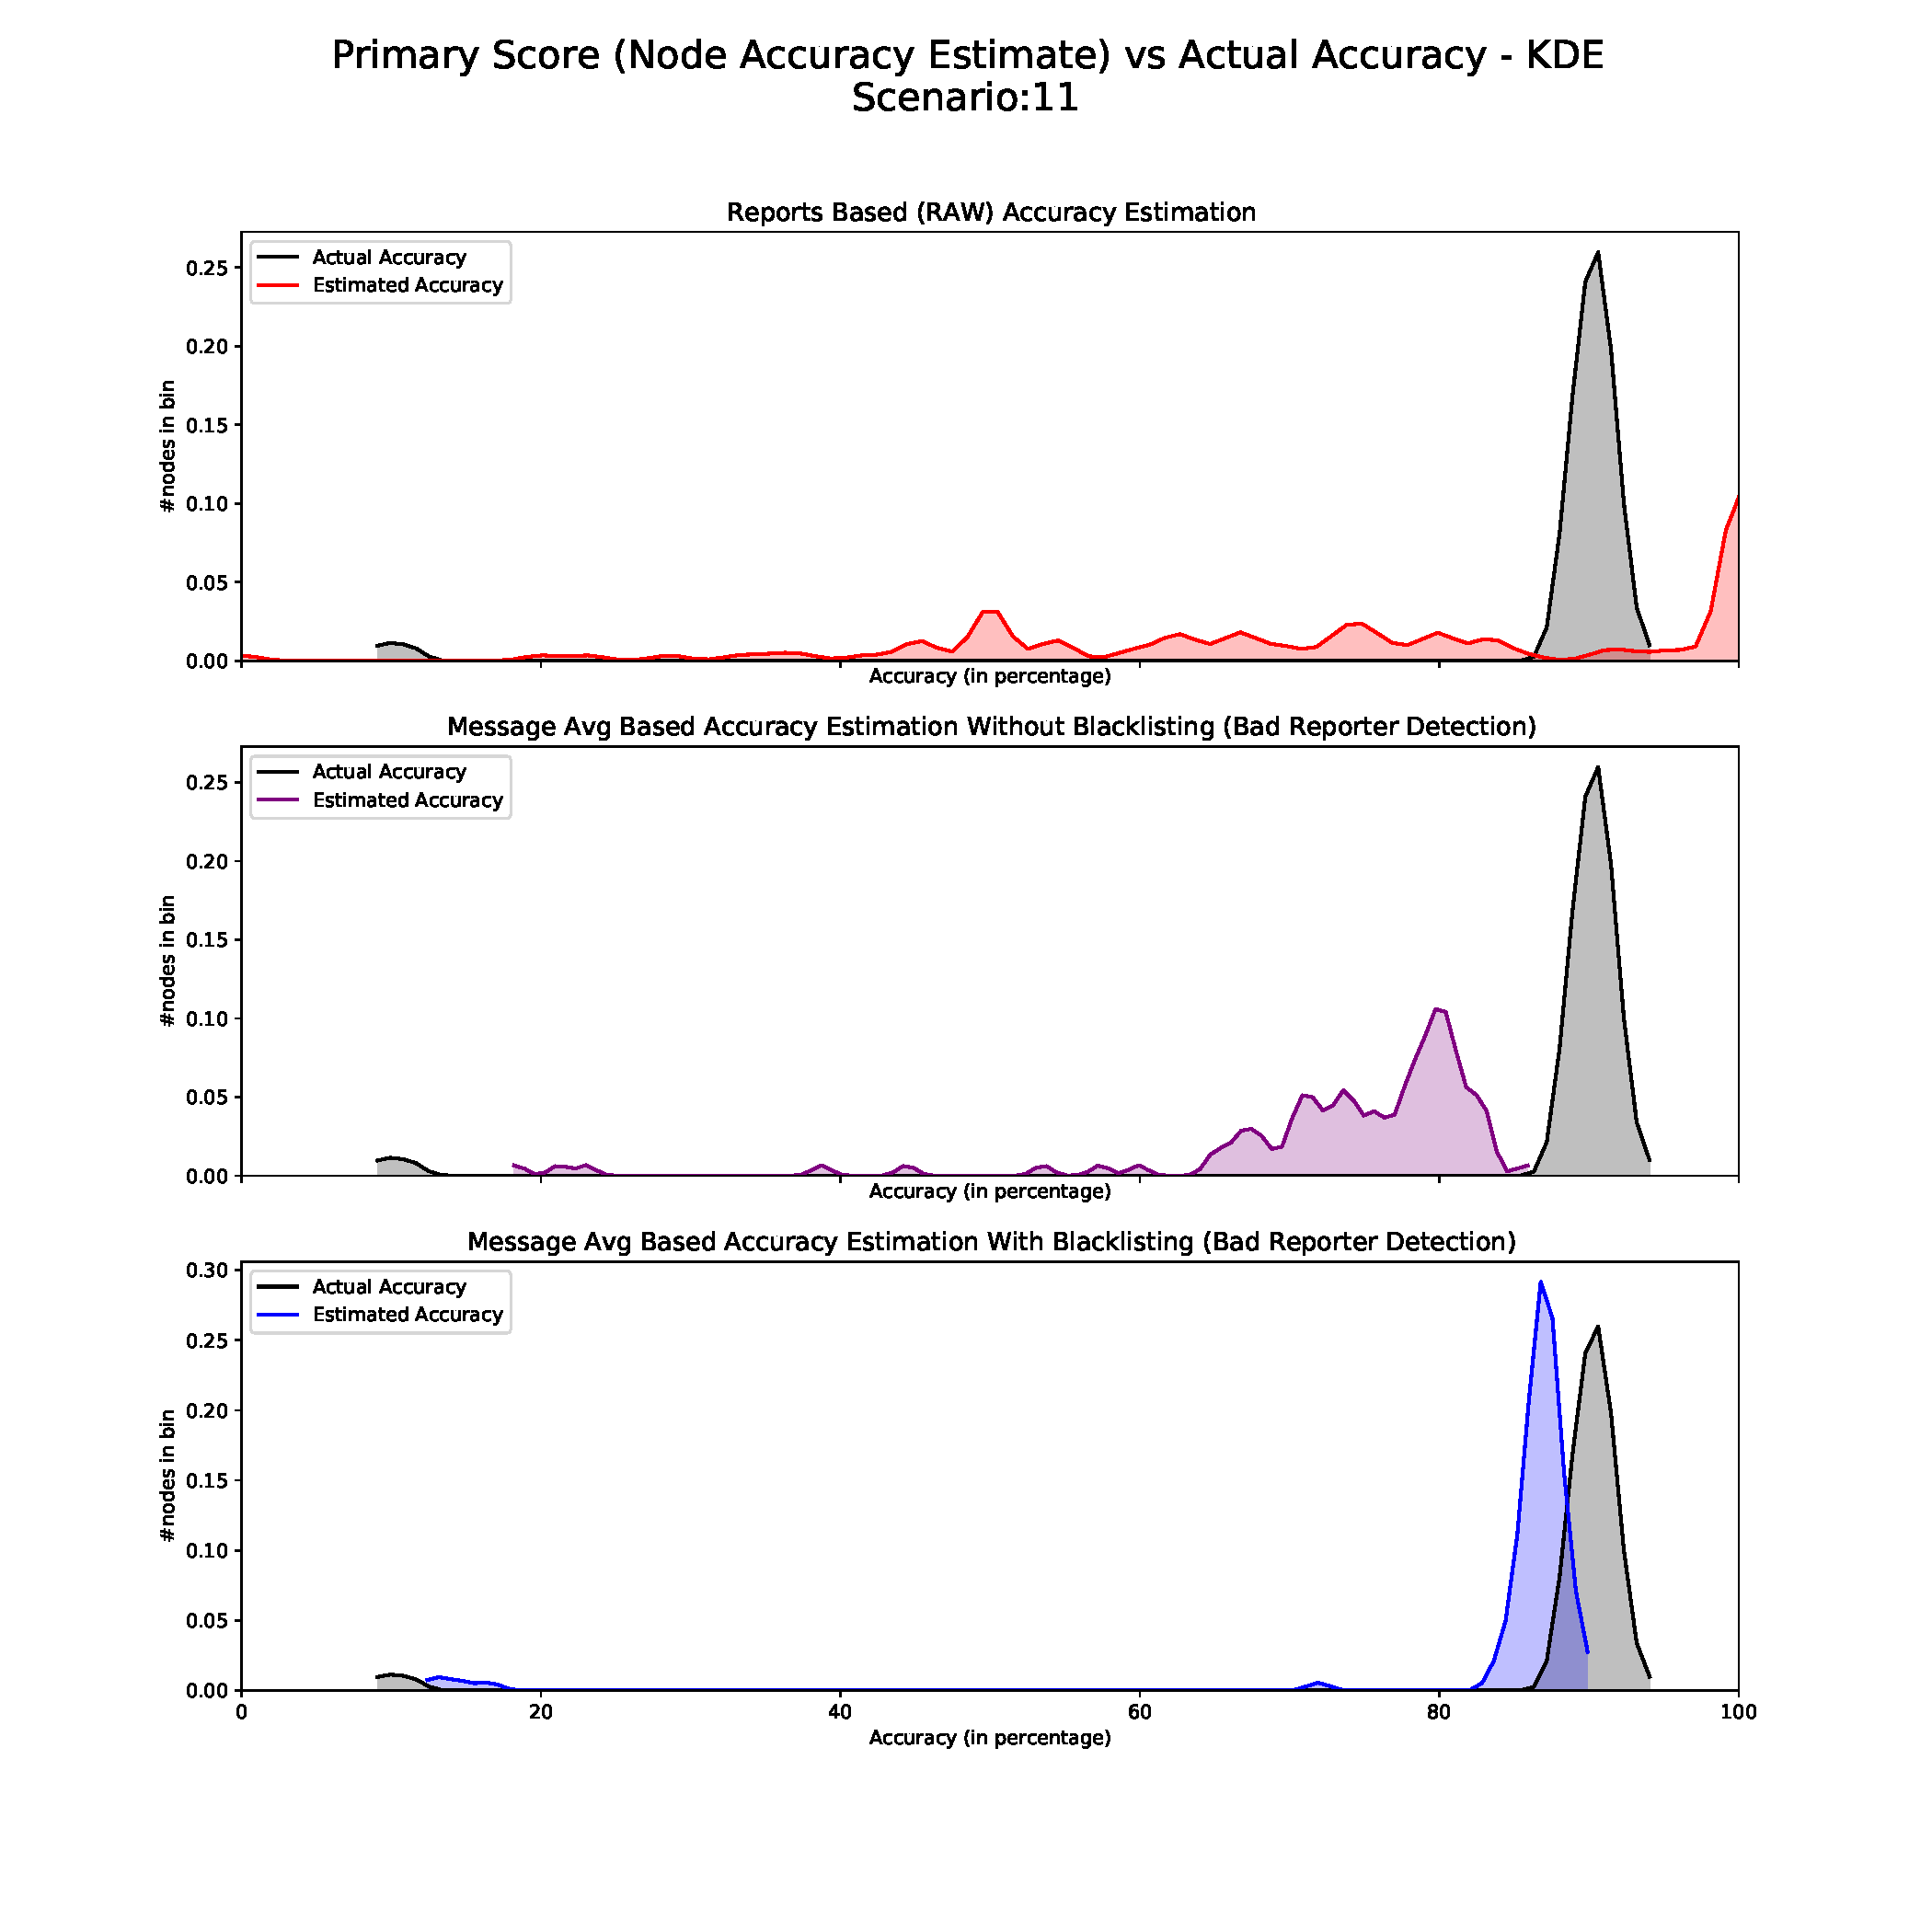
\includegraphics[width=0.5\linewidth, trim={80 95 100 100}, clip]{images/SCN11_PrimaryScoreKDEComparitive.pdf}
	}
	\hfill
	\subfloat[]{
		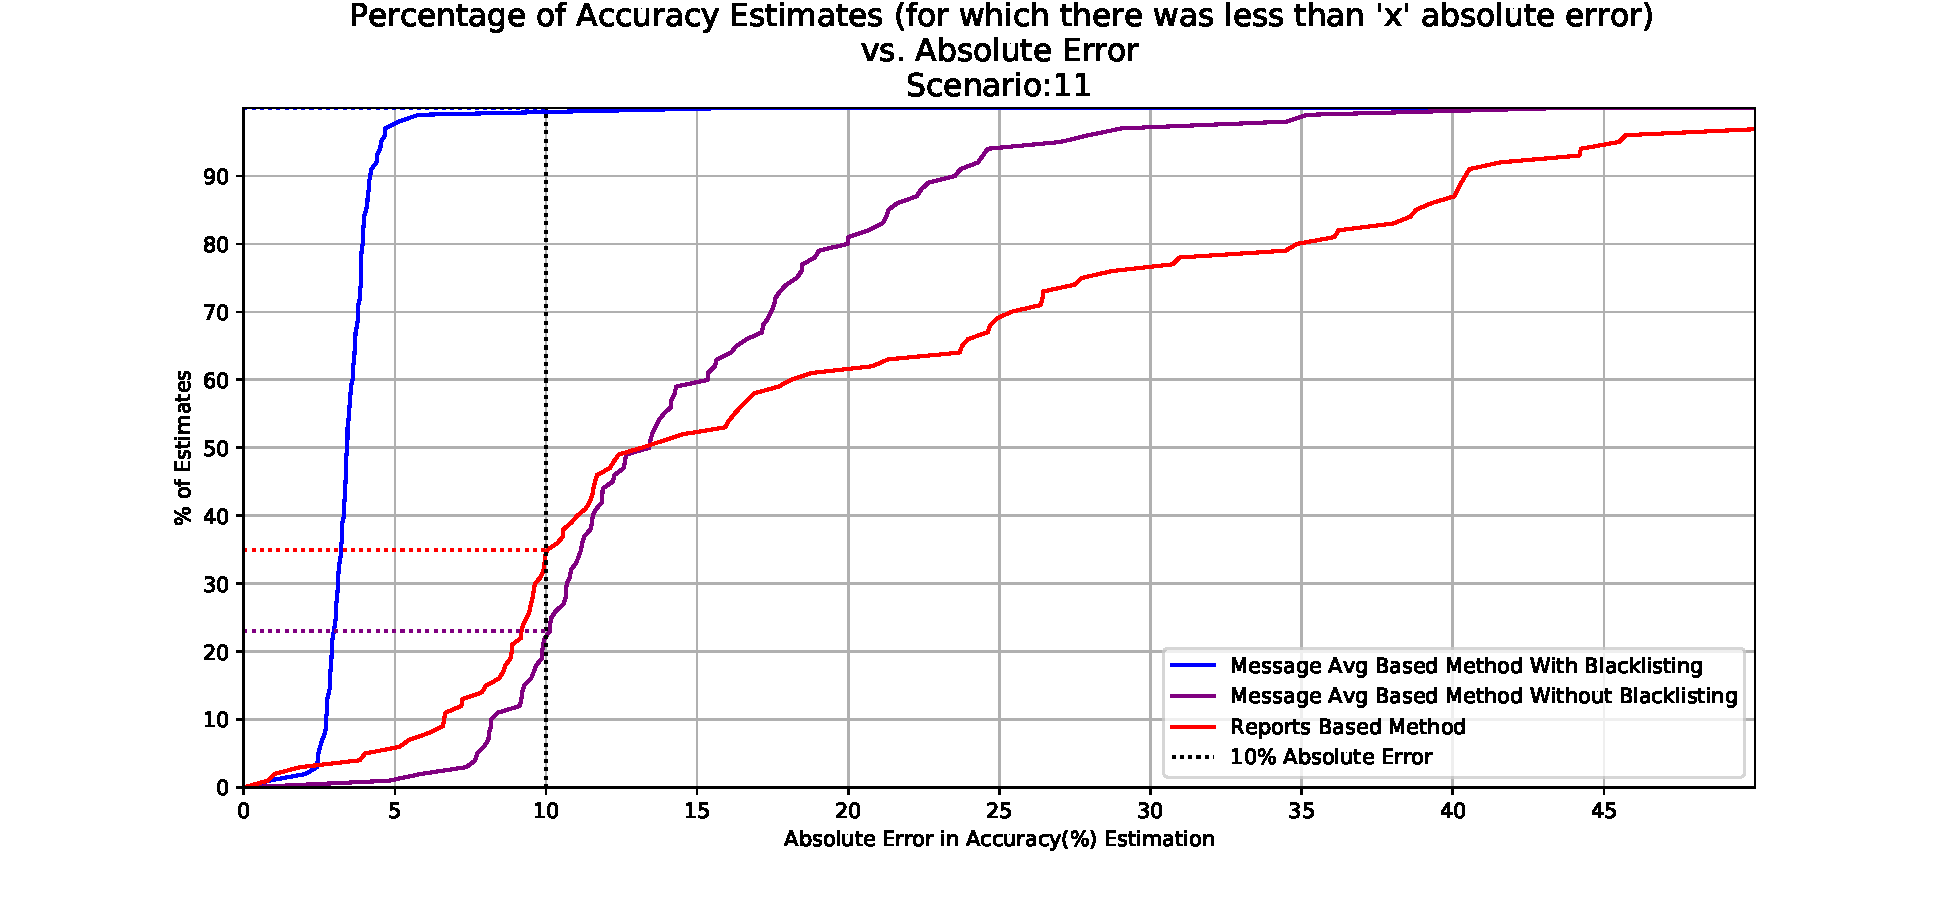
\includegraphics[width=0.5\linewidth, trim={80 25 90 50}, clip]{images/SCN11_AbsoluteErrorsInEstimationComparison.pdf}
	}
	\subfloat[]{
		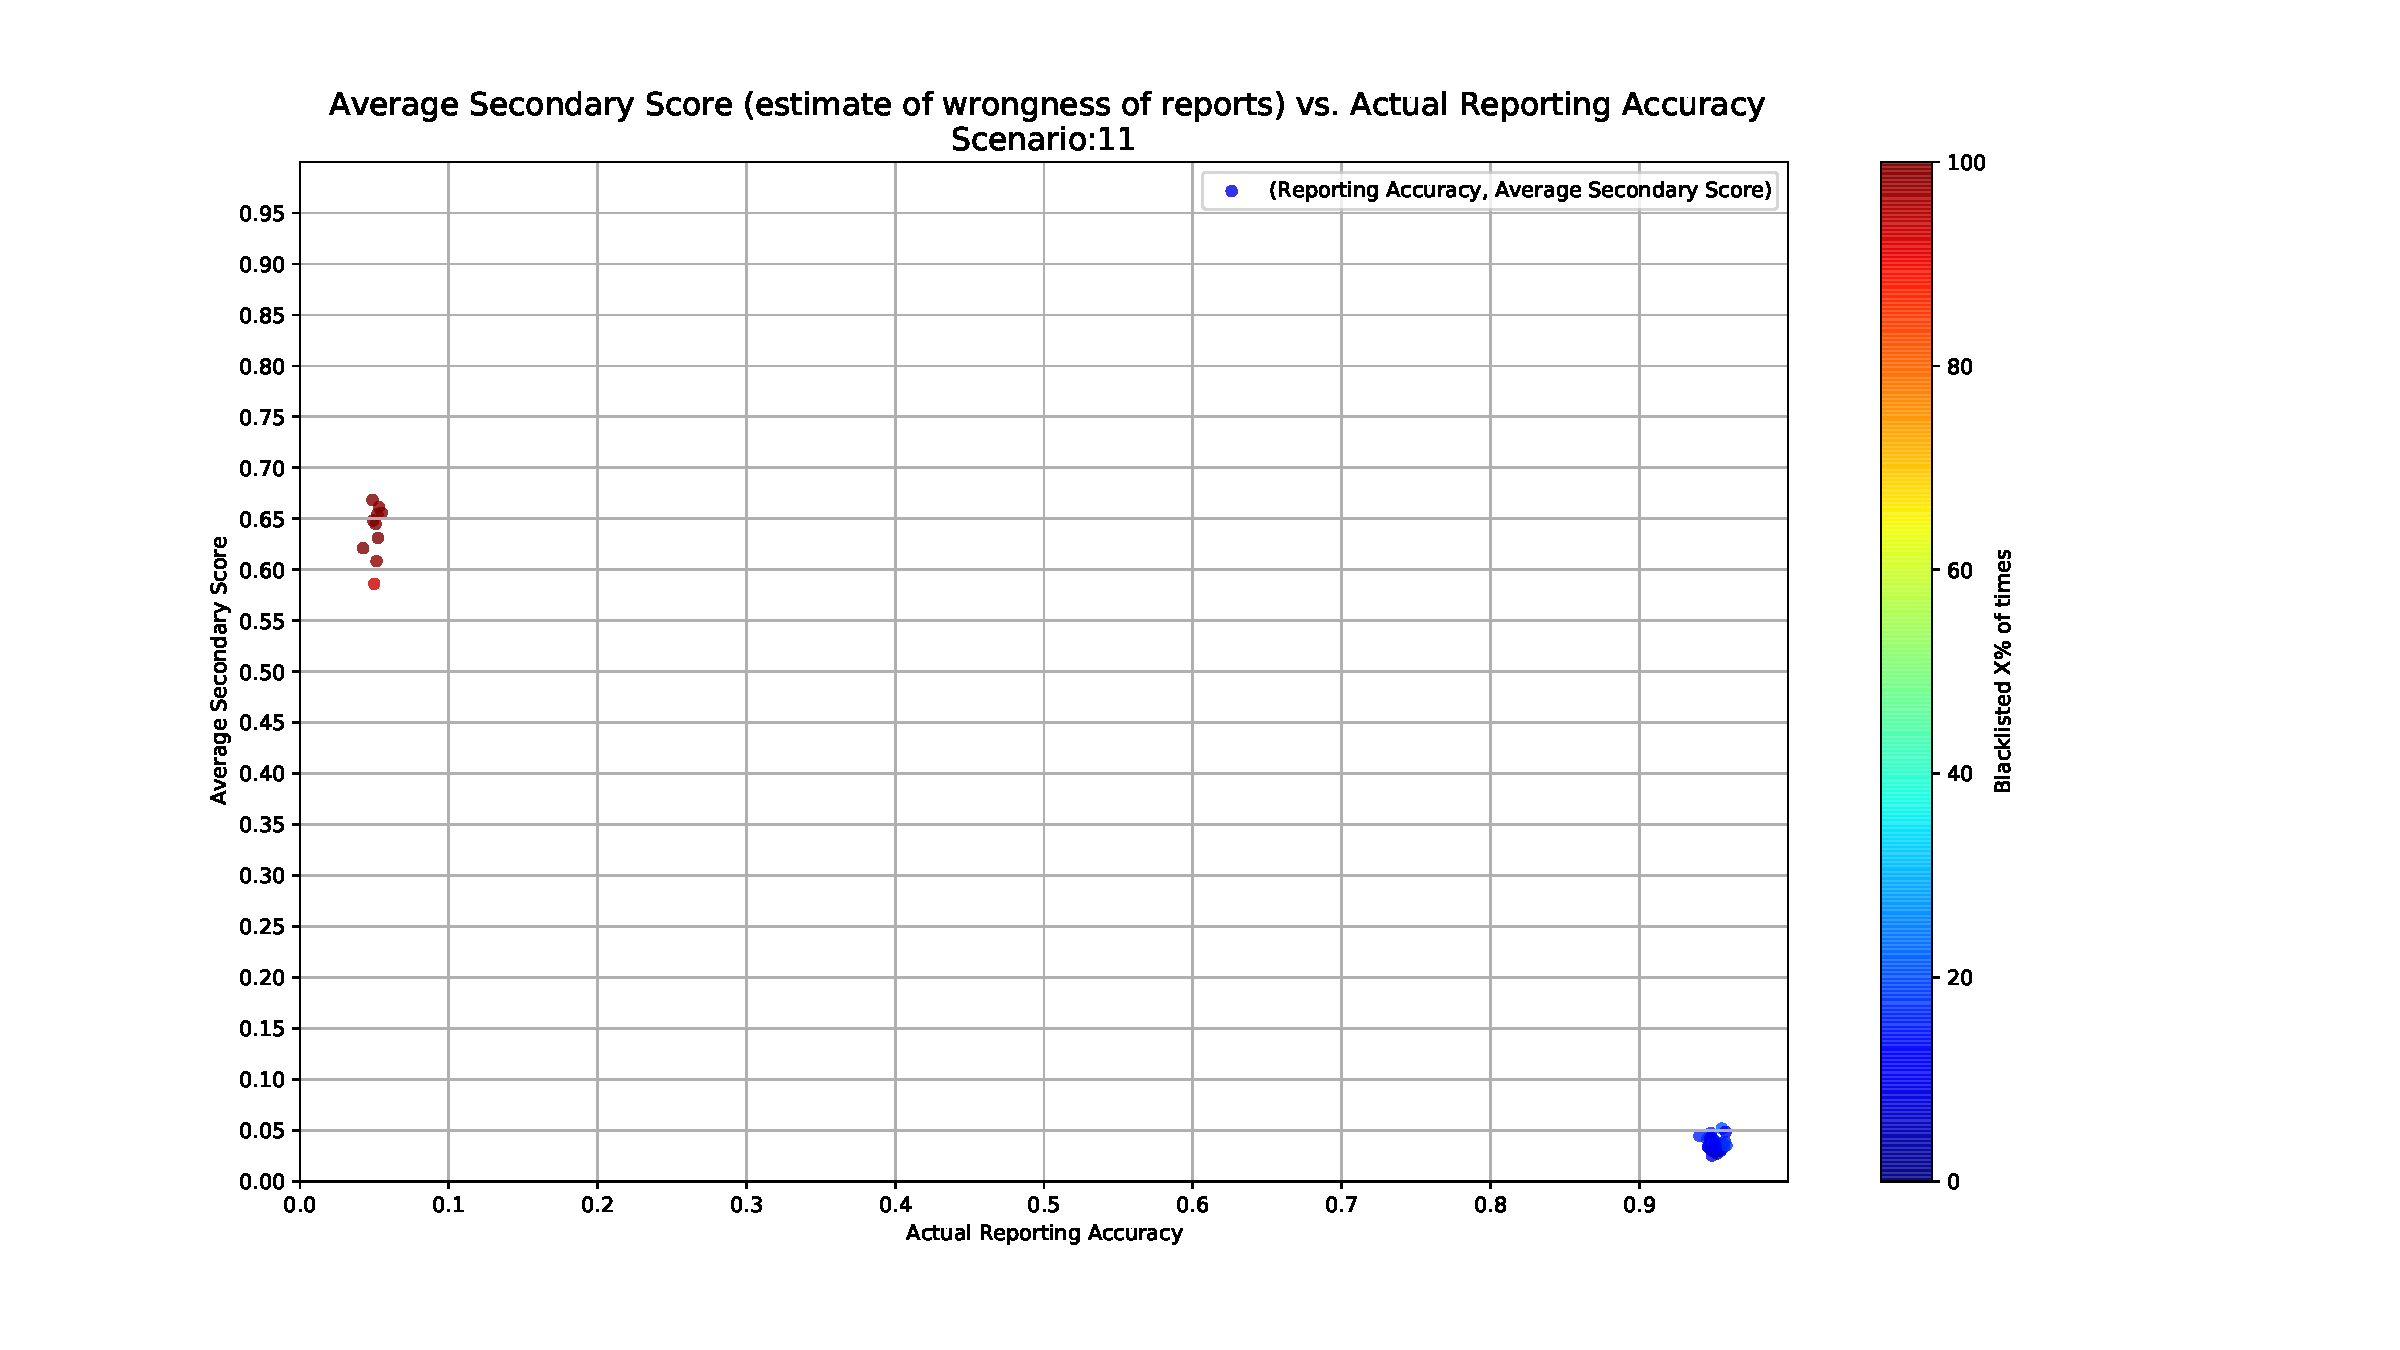
\includegraphics[width=0.5\linewidth,trim={100 50 185 72}, clip]{images/SCN11_ReportingAccuracy_Vs_AvgSecondaryScore.pdf}
	}
\end{figure*}
\begin{figure*}[!ht]
	\caption{Graphs for Results of Scenario 12. (a) Primary Score vs. Actual Accuracy - Scatter plot. (b) Primary Score and Actual Accuracy KDE. An Indicator of closeness of estimates. (c) Absolute error (difference between actual accuracy of node and estimated accuracy) vs. Percentage of nodes for which there was less than 'x'\% error. (d) Mean Secondary Score vs. Accuracy of Reports Sent - Scatter plot.}
	\label{fig:apdx:sc12}
	\centering
	\subfloat[]{
		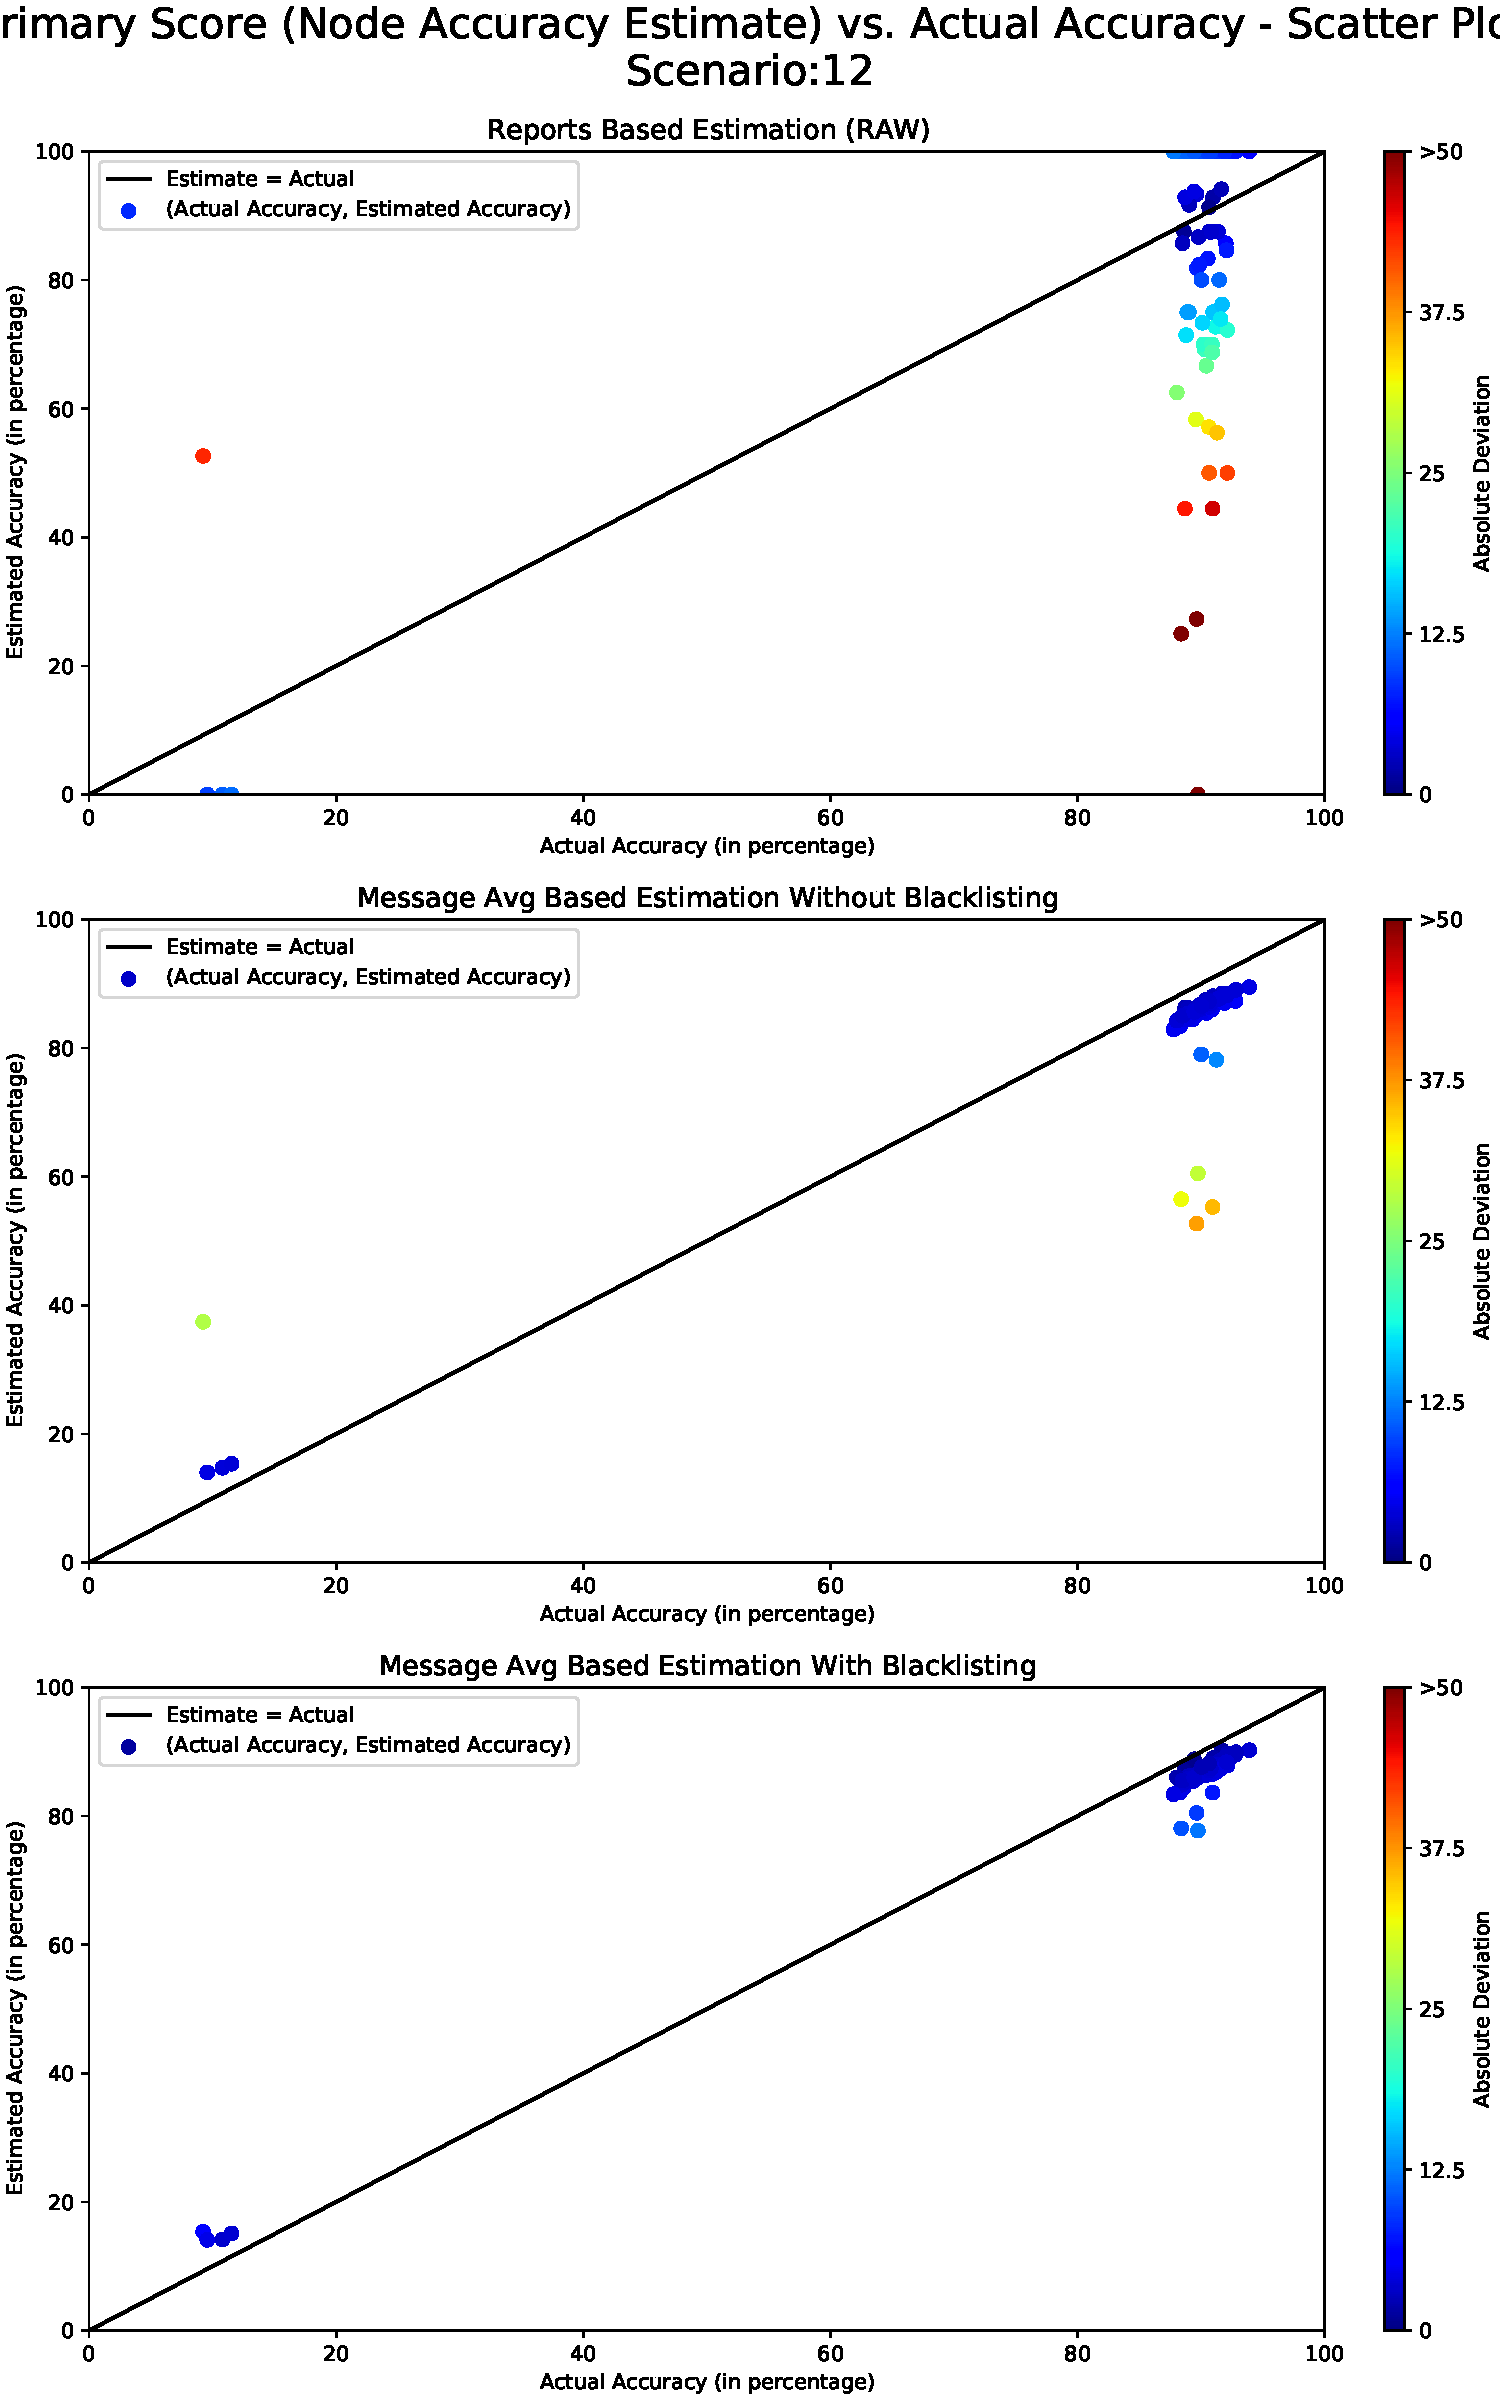
\includegraphics[width=0.5\linewidth, trim={0 5 15 50}, clip]{images/SCN12_PrimaryScoreVsActualAccuracyComparitive.pdf}
	}
	\subfloat[]{
		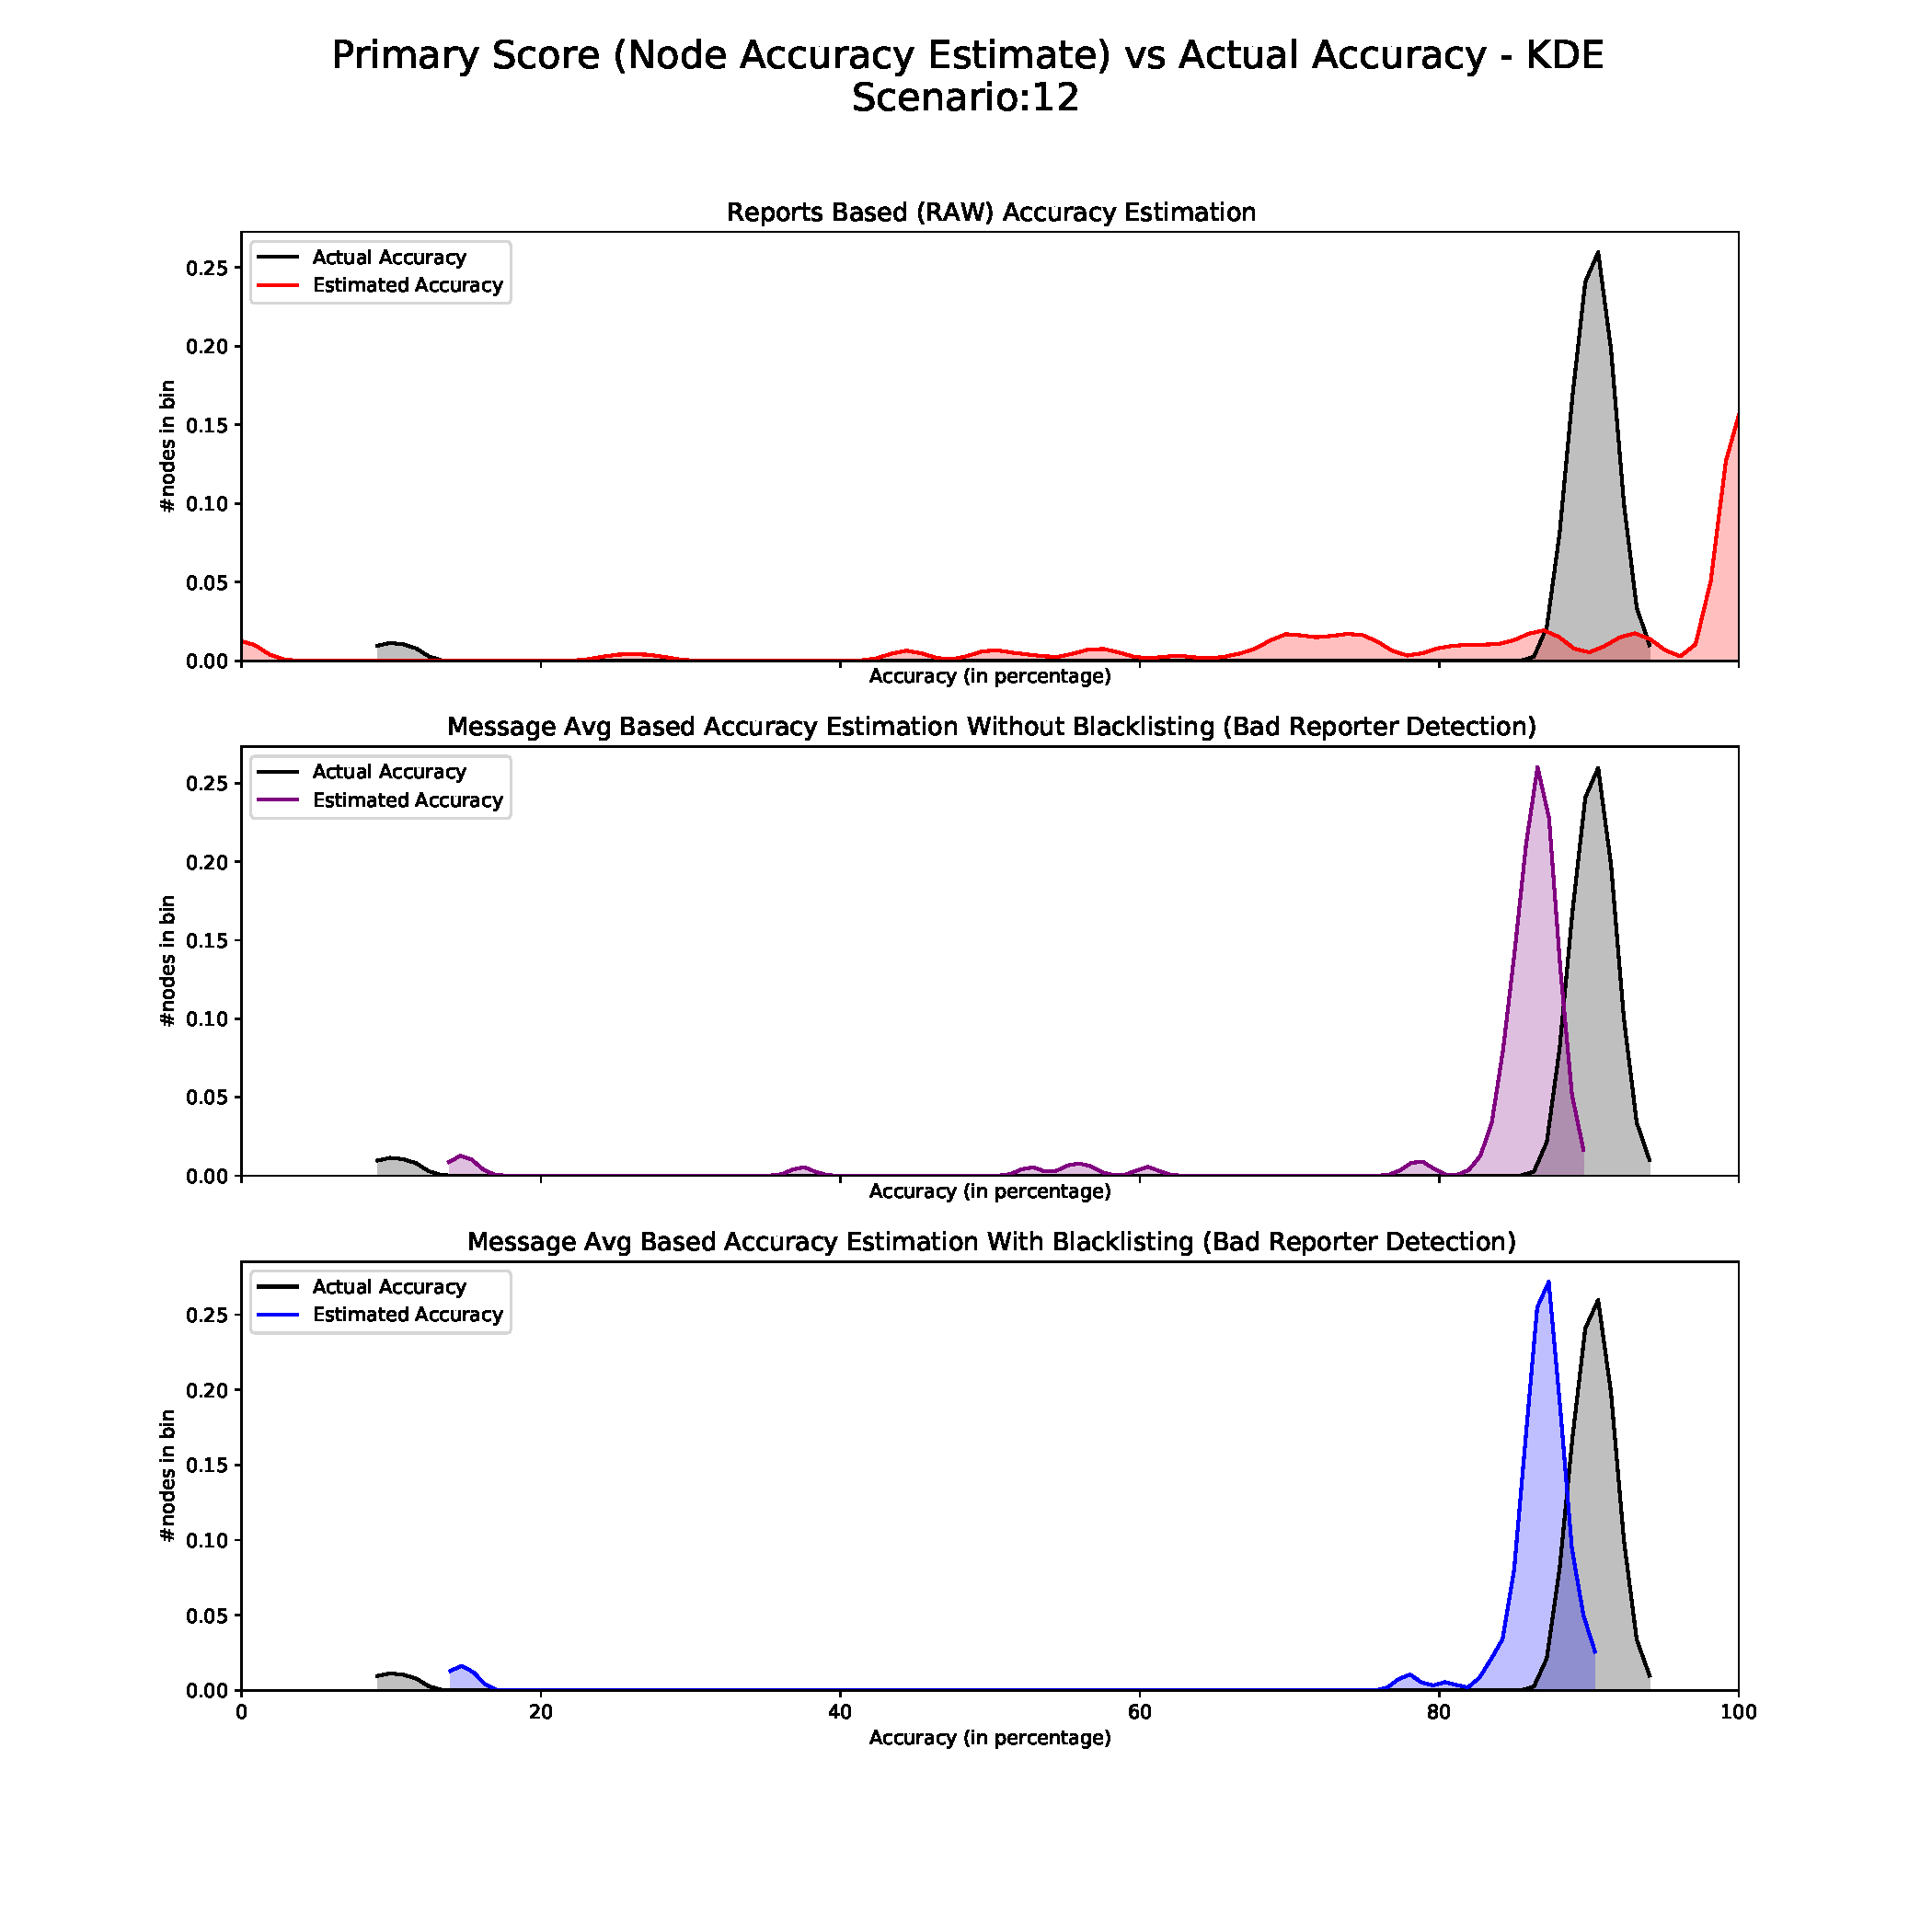
\includegraphics[width=0.5\linewidth, trim={80 95 100 100}, clip]{images/SCN12_PrimaryScoreKDEComparitive.pdf}
	}
	\hfill
	\subfloat[]{
		\includegraphics[width=0.5\linewidth, trim={80 25 90 50}, clip]{images/SCN12_AbsoluteErrorsInEstimationComparison.pdf}
	}
	\subfloat[]{
		\includegraphics[width=0.5\linewidth,trim={100 50 185 72}, clip]{images/SCN12_ReportingAccuracy_Vs_AvgSecondaryScore.pdf}
	}
\end{figure*}
\fi
% use section* for acknowledgment
%\section*{Acknowledgment}
%dsdfsfsdf


% Can use something like this to put references on a page
% by themselves when using endfloat and the captionsoff option.
\ifCLASSOPTIONcaptionsoff
  \newpage
\fi



% trigger a \newpage just before the given reference
% number - used to balance the columns on the last page
% adjust value as needed - may need to be readjusted if
% the document is modified later
%\IEEEtriggeratref{8}
% The "triggered" command can be changed if desired:
%\IEEEtriggercmd{\enlargethispage{-5in}}

% references section

% can use a bibliography generated by BibTeX as a .bbl file
% BibTeX documentation can be easily obtained at:
% http://mirror.ctan.org/biblio/bibtex/contrib/doc/
% The IEEEtran BibTeX style support page is at:
% http://www.michaelshell.org/tex/ieeetran/bibtex/
\newpage
\vfill\hfill
\newpage
\hfill
\bibliographystyle{IEEEtran}
% argument is your BibTeX string definitions and bibliography database(s)

\bibliography{IEEEabrv,myBib}
%
% <OR> manually copy in the resultant .bbl file
% set second argument of \begin to the number of references
% (used to reserve space for the reference number labels box)
%\begin{thebibliography}{1}

%\bibitem{IEEEhowto:kopka}
%H.~Kopka and P.~W. Daly, \emph{A Guide to \LaTeX}, 3rd~ed.\hskip 1em plus
%  0.5em minus 0.4em\relax Harlow, England: Addison-Wesley, 1999.
%
%\end{thebibliography}

% biography section
% 
% If you have an EPS/PDF photo (graphicx package needed) extra braces are
% needed around the contents of the optional argument to biography to prevent
% the LaTeX parser from getting confused when it sees the complicated
% \includegraphics command within an optional argument. (You could create
% your own custom macro containing the \includegraphics command to make things
% simpler here.)
%\begin{IEEEbiography}[{\includegraphics[width=1in,height=1.25in,clip,keepaspectratio]{mshell}}]{Michael Shell}
% or if you just want to reserve a space for a photo:
\newpage

\begin{IEEEbiography}[{\includegraphics[width=1in,height=1.25in,clip,keepaspectratio]{images/rohanBW.png}}]{Rohan Dahiya}
Rohan Dahiya was born in New Delhi, India in 1997. He is currently pursuing the B.Tech. degree in computer science and engineering with specialisation in information security from Vellore Institute of Technology, TN, India. \\ He has worked as an Intern at Volon Cyber Security in the summer of 2018 and at GAP IT Services India in the summer of 2019. He is was a Visiting Researcher at Deakin University, Burwood, VIC, Australia from December 2019 till May 2020.
\end{IEEEbiography}

\begin{IEEEbiography}[{\includegraphics[width=1in,height=1.25in,clip,keepaspectratio]{images/FrankJiangPhoto.pdf}}]{Frank Jiang}
Frank Jiang received the master’s degree in computer science from the University of New South Wales (UNSW), Australia and the Ph.D. degree from The University of Technology Sydney, Australia. He gained three and a half years of postdoctoral research experience at UNSW. He is currently a Senior Lecturer of cyber security with the School of Info Technology Campus, Deakin University, Australia. He has published over 100 highly reputed SCI/EI indexed journal/conferences papers. His main research interests include data-driven cyber security, predictive analytics, biologically inspired learning mechanism, and its application in the complex information security systems.
\end{IEEEbiography}

% insert where needed to balance the two columns on the last page with
% biographies
%\newpage

\begin{IEEEbiography}[{\includegraphics[width=1in,height=1.25in,clip,keepaspectratio]{images/RobinDossPhoto.pdf}}]{Robin Doss}
Robin Doss (Senior Member, IEEE) received the B.E. degree in electronics and communication engineering from the University of Madras, India, and the master’s and Ph.D. degrees from the Royal Melbourne Institute of Technology (RMIT), Australia. He was a part of the Technical Services Group, Ericsson Australia, and a Research Engineer at RMIT University. He is currently a Professor of information technology and the Deputy Head of the School of Information Technology, Deakin University, Australia. He leads a team of researchers and Ph.D. students in the broad areas of communication systems and cybersecurity with a focus on emerging domains, such as the IoT, pervasive computing, applied machine learning, and ambient intelligence. His research has been funded by the National Security Science and Technology Branch of the Office of National Security in collaboration with the Defence Signals Directorate, the Australian Research Council, and industry partners. He is the Founding Chair of the Future Network Systems and Security Conference series. He is also an Associate Editor of the journal of Cyber-Physical Systems.
\end{IEEEbiography}

% You can push biographies down or up by placing
% a \vfill before or after them. The appropriate
% use of \vfill depends on what kind of text is
% on the last page and whether or not the columns
% are being equalized.

%\vfill

% Can be used to pull up biographies so that the bottom of the last one
% is flush with the other column.
%\enlargethispage{-5in}


% that's all folks
\end{document}


